\documentclass[twoside]{book}

% Packages required by doxygen
\usepackage{fixltx2e}
\usepackage{calc}
\usepackage{doxygen}
\usepackage[export]{adjustbox} % also loads graphicx
\usepackage{graphicx}
\usepackage[utf8]{inputenc}
\usepackage{makeidx}
\usepackage{multicol}
\usepackage{multirow}
\PassOptionsToPackage{warn}{textcomp}
\usepackage{textcomp}
\usepackage[nointegrals]{wasysym}
\usepackage[table]{xcolor}

% Font selection
\usepackage[T1]{fontenc}
\usepackage[scaled=.90]{helvet}
\usepackage{courier}
\usepackage{amssymb}
\usepackage{sectsty}
\renewcommand{\familydefault}{\sfdefault}
\allsectionsfont{%
  \fontseries{bc}\selectfont%
  \color{darkgray}%
}
\renewcommand{\DoxyLabelFont}{%
  \fontseries{bc}\selectfont%
  \color{darkgray}%
}
\newcommand{\+}{\discretionary{\mbox{\scriptsize$\hookleftarrow$}}{}{}}

% Page & text layout
\usepackage{geometry}
\geometry{%
  a4paper,%
  top=2.5cm,%
  bottom=2.5cm,%
  left=2.5cm,%
  right=2.5cm%
}
\tolerance=750
\hfuzz=15pt
\hbadness=750
\setlength{\emergencystretch}{15pt}
\setlength{\parindent}{0cm}
\setlength{\parskip}{3ex plus 2ex minus 2ex}
\makeatletter
\renewcommand{\paragraph}{%
  \@startsection{paragraph}{4}{0ex}{-1.0ex}{1.0ex}{%
    \normalfont\normalsize\bfseries\SS@parafont%
  }%
}
\renewcommand{\subparagraph}{%
  \@startsection{subparagraph}{5}{0ex}{-1.0ex}{1.0ex}{%
    \normalfont\normalsize\bfseries\SS@subparafont%
  }%
}
\makeatother

% Headers & footers
\usepackage{fancyhdr}
\pagestyle{fancyplain}
\fancyhead[LE]{\fancyplain{}{\bfseries\thepage}}
\fancyhead[CE]{\fancyplain{}{}}
\fancyhead[RE]{\fancyplain{}{\bfseries\leftmark}}
\fancyhead[LO]{\fancyplain{}{\bfseries\rightmark}}
\fancyhead[CO]{\fancyplain{}{}}
\fancyhead[RO]{\fancyplain{}{\bfseries\thepage}}
\fancyfoot[LE]{\fancyplain{}{}}
\fancyfoot[CE]{\fancyplain{}{}}
\fancyfoot[RE]{\fancyplain{}{\bfseries\scriptsize Generated by Doxygen }}
\fancyfoot[LO]{\fancyplain{}{\bfseries\scriptsize Generated by Doxygen }}
\fancyfoot[CO]{\fancyplain{}{}}
\fancyfoot[RO]{\fancyplain{}{}}
\renewcommand{\footrulewidth}{0.4pt}
\renewcommand{\chaptermark}[1]{%
  \markboth{#1}{}%
}
\renewcommand{\sectionmark}[1]{%
  \markright{\thesection\ #1}%
}

% Indices & bibliography
\usepackage{natbib}
\usepackage[titles]{tocloft}
\setcounter{tocdepth}{3}
\setcounter{secnumdepth}{5}
\makeindex

% Hyperlinks (required, but should be loaded last)
\usepackage{ifpdf}
\ifpdf
  \usepackage[pdftex,pagebackref=true]{hyperref}
\else
  \usepackage[ps2pdf,pagebackref=true]{hyperref}
\fi
\hypersetup{%
  colorlinks=true,%
  linkcolor=blue,%
  citecolor=blue,%
  unicode%
}

% Custom commands
\newcommand{\clearemptydoublepage}{%
  \newpage{\pagestyle{empty}\cleardoublepage}%
}

\usepackage{caption}
\captionsetup{labelsep=space,justification=centering,font={bf},singlelinecheck=off,skip=4pt,position=top}

%===== C O N T E N T S =====

\begin{document}

% Titlepage & ToC
\hypersetup{pageanchor=false,
             bookmarksnumbered=true,
             pdfencoding=unicode
            }
\pagenumbering{alph}
\begin{titlepage}
\vspace*{7cm}
\begin{center}%
{\Large \#F\+MF \\[1ex]\large v3.\+0 }\\
\vspace*{1cm}
{\large Generated by Doxygen 1.8.13}\\
\end{center}
\end{titlepage}
\clearemptydoublepage
\pagenumbering{roman}
\tableofcontents
\clearemptydoublepage
\pagenumbering{arabic}
\hypersetup{pageanchor=true}

%--- Begin generated contents ---
\chapter{Hierarchical Index}
\section{Class Hierarchy}
This inheritance list is sorted roughly, but not completely, alphabetically\+:\begin{DoxyCompactList}
\item \contentsline{section}{Boundary}{\pageref{class_boundary}}{}
\item \contentsline{section}{Character}{\pageref{class_character}}{}
\item \contentsline{section}{Collision\+Detection}{\pageref{class_collision_detection}}{}
\item \contentsline{section}{Delay\+Component}{\pageref{class_delay_component}}{}
\item \contentsline{section}{Destroyed\+Object\+Outside\+Scene}{\pageref{class_destroyed_object_outside_scene}}{}
\item \contentsline{section}{Display\+Manager}{\pageref{class_display_manager}}{}
\item \contentsline{section}{Draw\+Game\+Object}{\pageref{class_draw_game_object}}{}
\item enable\+\_\+shared\+\_\+from\+\_\+this\begin{DoxyCompactList}
\item \contentsline{section}{Game\+Object}{\pageref{class_game_object}}{}
\begin{DoxyCompactList}
\item \contentsline{section}{Enemy\+Controller}{\pageref{class_enemy_controller}}{}
\item \contentsline{section}{Physics\+Object}{\pageref{class_physics_object}}{}
\begin{DoxyCompactList}
\item \contentsline{section}{Enemy}{\pageref{class_enemy}}{}
\item \contentsline{section}{Player}{\pageref{class_player}}{}
\item \contentsline{section}{Projectile}{\pageref{class_projectile}}{}
\end{DoxyCompactList}
\item \contentsline{section}{Splash\+Screen}{\pageref{class_splash_screen}}{}
\end{DoxyCompactList}
\item \contentsline{section}{Scene}{\pageref{class_scene}}{}
\end{DoxyCompactList}
\item \contentsline{section}{Event\+Manager}{\pageref{class_event_manager}}{}
\item \contentsline{section}{Failed\+To\+Load\+Texture}{\pageref{class_failed_to_load_texture}}{}
\item \contentsline{section}{Game\+Manager}{\pageref{class_game_manager}}{}
\item \contentsline{section}{Game\+Time}{\pageref{class_game_time}}{}
\item \contentsline{section}{Graphic\+Name\+Reservedfoo\+Null\+Graphic}{\pageref{class_graphic_name_reservedfoo_null_graphic}}{}
\item \contentsline{section}{Graphic\+Name\+Reservedfor\+Null\+Graphic}{\pageref{class_graphic_name_reservedfor_null_graphic}}{}
\item \contentsline{section}{Graphic\+Object}{\pageref{class_graphic_object}}{}
\item \contentsline{section}{Input}{\pageref{class_input}}{}
\item \contentsline{section}{Movable\+Object}{\pageref{class_movable_object}}{}
\item \contentsline{section}{My\+Singleton}{\pageref{class_my_singleton}}{}
\item \contentsline{section}{Scene\+Doesnt\+Exist}{\pageref{class_scene_doesnt_exist}}{}
\item \contentsline{section}{Shoot\+Component}{\pageref{class_shoot_component}}{}
\item \contentsline{section}{Singleton\+Exists}{\pageref{class_singleton_exists}}{}
\item \contentsline{section}{Sprite\+Info}{\pageref{struct_sprite_info}}{}
\item \contentsline{section}{Update\+Game\+Object\+Display}{\pageref{class_update_game_object_display}}{}
\item \contentsline{section}{Vector2D$<$ T $>$}{\pageref{class_vector2_d}}{}
\item \contentsline{section}{Vector2D$<$ double $>$}{\pageref{class_vector2_d}}{}
\item \contentsline{section}{Vector2\+D\+Convert}{\pageref{class_vector2_d_convert}}{}
\item \contentsline{section}{Vector\+Size\+Error}{\pageref{class_vector_size_error}}{}
\item \contentsline{section}{Window\+Settings}{\pageref{struct_window_settings}}{}
\item \contentsline{section}{xy\+Vector}{\pageref{structxy_vector}}{}
\end{DoxyCompactList}

\chapter{Class Index}
\section{Class List}
Here are the classes, structs, unions and interfaces with brief descriptions\+:\begin{DoxyCompactList}
\item\contentsline{section}{\hyperlink{class_boundary}{Boundary} }{\pageref{class_boundary}}{}
\item\contentsline{section}{\hyperlink{class_character}{Character} \\*Entire class needs to change }{\pageref{class_character}}{}
\item\contentsline{section}{\hyperlink{class_collision_detection}{Collision\+Detection} }{\pageref{class_collision_detection}}{}
\item\contentsline{section}{\hyperlink{class_delay_component}{Delay\+Component} }{\pageref{class_delay_component}}{}
\item\contentsline{section}{\hyperlink{class_destroyed_object_outside_scene}{Destroyed\+Object\+Outside\+Scene} }{\pageref{class_destroyed_object_outside_scene}}{}
\item\contentsline{section}{\hyperlink{class_display_manager}{Display\+Manager} \\*Display manager is in charge of running and managing the presentation layer }{\pageref{class_display_manager}}{}
\item\contentsline{section}{\hyperlink{class_enemy}{Enemy} }{\pageref{class_enemy}}{}
\item\contentsline{section}{\hyperlink{class_enemy_controller}{Enemy\+Controller} \\*Needs copy constructor and assignment opperator }{\pageref{class_enemy_controller}}{}
\item\contentsline{section}{\hyperlink{class_event_manager}{Event\+Manager} \\*Can be converted into a singleton }{\pageref{class_event_manager}}{}
\item\contentsline{section}{\hyperlink{class_failed_to_load_texture}{Failed\+To\+Load\+Texture} }{\pageref{class_failed_to_load_texture}}{}
\item\contentsline{section}{\hyperlink{class_game_manager}{Game\+Manager} \\*Needs to be converted into a singleton }{\pageref{class_game_manager}}{}
\item\contentsline{section}{\hyperlink{class_game_object}{Game\+Object} }{\pageref{class_game_object}}{}
\item\contentsline{section}{\hyperlink{class_game_time}{Game\+Time} }{\pageref{class_game_time}}{}
\item\contentsline{section}{\hyperlink{class_graphic_object}{Graphic\+Object} }{\pageref{class_graphic_object}}{}
\item\contentsline{section}{\hyperlink{class_input}{Input} }{\pageref{class_input}}{}
\item\contentsline{section}{\hyperlink{class_movable_object}{Movable\+Object} }{\pageref{class_movable_object}}{}
\item\contentsline{section}{\hyperlink{class_my_singleton}{My\+Singleton} }{\pageref{class_my_singleton}}{}
\item\contentsline{section}{\hyperlink{class_physics_object}{Physics\+Object} \\*May not need to inherit from \hyperlink{class_game_object}{Game\+Object} }{\pageref{class_physics_object}}{}
\item\contentsline{section}{\hyperlink{class_player}{Player} \\*\hyperlink{class_character}{Character} rework required here as well }{\pageref{class_player}}{}
\item\contentsline{section}{\hyperlink{class_projectile}{Projectile} }{\pageref{class_projectile}}{}
\item\contentsline{section}{\hyperlink{class_scene}{Scene} }{\pageref{class_scene}}{}
\item\contentsline{section}{\hyperlink{class_scene_doesnt_exist}{Scene\+Doesnt\+Exist} }{\pageref{class_scene_doesnt_exist}}{}
\item\contentsline{section}{\hyperlink{class_shoot_component}{Shoot\+Component} }{\pageref{class_shoot_component}}{}
\item\contentsline{section}{\hyperlink{class_singleton_exists}{Singleton\+Exists} }{\pageref{class_singleton_exists}}{}
\item\contentsline{section}{\hyperlink{class_splash_screen}{Splash\+Screen} \\*Requires Seperation of Concerns }{\pageref{class_splash_screen}}{}
\item\contentsline{section}{\hyperlink{struct_sprite_info}{Sprite\+Info} }{\pageref{struct_sprite_info}}{}
\item\contentsline{section}{\hyperlink{class_vector2_d}{Vector2\+D$<$ T $>$} }{\pageref{class_vector2_d}}{}
\item\contentsline{section}{\hyperlink{class_vector2_d_convert}{Vector2\+D\+Convert} }{\pageref{class_vector2_d_convert}}{}
\item\contentsline{section}{\hyperlink{class_vector_size_error}{Vector\+Size\+Error} }{\pageref{class_vector_size_error}}{}
\item\contentsline{section}{\hyperlink{struct_window_settings}{Window\+Settings} \\*Must be moved into a database class }{\pageref{struct_window_settings}}{}
\item\contentsline{section}{\hyperlink{structxy_vector}{xy\+Vector} }{\pageref{structxy_vector}}{}
\end{DoxyCompactList}

\chapter{Class Documentation}
\hypertarget{class_application}{}\section{Application Class Reference}
\label{class_application}\index{Application@{Application}}


\hyperlink{class_application}{Application} acts as the main interface between the game objects and the game system. It allows game objects to access information about the current state of the game and to load scenes when certain conditions are met. It also provides game objects with access to the \hyperlink{class_repository}{Repository} object so that new game\+Objects can be instantiated into the current scene of the game.  




{\ttfamily \#include $<$Application.\+h$>$}

\subsection*{Public Member Functions}
\begin{DoxyCompactItemize}
\item 
\mbox{\Hypertarget{class_application_aa144608f9dff238ac87b51ae86cb414c}\label{class_application_aa144608f9dff238ac87b51ae86cb414c}} 
{\bfseries Application} (std\+::shared\+\_\+ptr$<$ \hyperlink{class_repositiory_interface}{Repositiory\+Interface} $>$ repository, std\+::shared\+\_\+ptr$<$ \hyperlink{class_game_manager}{Game\+Manager} $>$ game\+Manager=nullptr)
\item 
\mbox{\Hypertarget{class_application_a12f09b1508e9a881c97786cd07dab53a}\label{class_application_a12f09b1508e9a881c97786cd07dab53a}} 
void \hyperlink{class_application_a12f09b1508e9a881c97786cd07dab53a}{Run\+Application} ()
\begin{DoxyCompactList}\small\item\em Runs the application. \end{DoxyCompactList}\end{DoxyCompactItemize}
\subsection*{Static Public Member Functions}
\begin{DoxyCompactItemize}
\item 
static const std\+::shared\+\_\+ptr$<$ \hyperlink{class_repositiory_interface}{Repositiory\+Interface} $>$ \hyperlink{class_application_aa895ae75cdb47ab91584c32b0db0ca06}{get\+Game\+Repository} ()
\begin{DoxyCompactList}\small\item\em getter used to provide global access to the repository object used within the game system. The object is returned as a constant pointer to ensure that it cannot be changed. \end{DoxyCompactList}\item 
static void \hyperlink{class_application_ac73bbfb4af8c54f6ae777863b7fa7099}{Load\+Scene} (int index)
\begin{DoxyCompactList}\small\item\em Callback used to change the active scene to a different one at a particular index. \end{DoxyCompactList}\item 
\mbox{\Hypertarget{class_application_ab105d17f9a88e55db9b64b6b0e190b12}\label{class_application_ab105d17f9a88e55db9b64b6b0e190b12}} 
static void \hyperlink{class_application_ab105d17f9a88e55db9b64b6b0e190b12}{Close\+Application} ()
\begin{DoxyCompactList}\small\item\em Closes the Current application window. \end{DoxyCompactList}\item 
static const unsigned int \hyperlink{class_application_aaad856399fbe63c7f14a95fc59d0111f}{current\+Scene\+Index} ()
\begin{DoxyCompactList}\small\item\em obtains the scene index of the game \end{DoxyCompactList}\end{DoxyCompactItemize}
\subsection*{Static Private Attributes}
\begin{DoxyCompactItemize}
\item 
static std\+::shared\+\_\+ptr$<$ \hyperlink{class_repositiory_interface}{Repositiory\+Interface} $>$ \hyperlink{class_application_af7e1a832b2f8dbc3a283cb29f7a89c01}{\+\_\+repository} = nullptr
\item 
static std\+::shared\+\_\+ptr$<$ \hyperlink{class_game_manager}{Game\+Manager} $>$ \hyperlink{class_application_a4e102be4f84b7a22a159f6030bc022bd}{\+\_\+game\+Manager} = nullptr
\end{DoxyCompactItemize}


\subsection{Detailed Description}
\hyperlink{class_application}{Application} acts as the main interface between the game objects and the game system. It allows game objects to access information about the current state of the game and to load scenes when certain conditions are met. It also provides game objects with access to the \hyperlink{class_repository}{Repository} object so that new game\+Objects can be instantiated into the current scene of the game. 

\subsection{Member Function Documentation}
\mbox{\Hypertarget{class_application_aaad856399fbe63c7f14a95fc59d0111f}\label{class_application_aaad856399fbe63c7f14a95fc59d0111f}} 
\index{Application@{Application}!current\+Scene\+Index@{current\+Scene\+Index}}
\index{current\+Scene\+Index@{current\+Scene\+Index}!Application@{Application}}
\subsubsection{\texorpdfstring{current\+Scene\+Index()}{currentSceneIndex()}}
{\footnotesize\ttfamily const unsigned int Application\+::current\+Scene\+Index (\begin{DoxyParamCaption}{ }\end{DoxyParamCaption})\hspace{0.3cm}{\ttfamily [static]}}



obtains the scene index of the game 

\begin{DoxyReturn}{Returns}
Returns the scene index that is currently being used 
\end{DoxyReturn}
\mbox{\Hypertarget{class_application_aa895ae75cdb47ab91584c32b0db0ca06}\label{class_application_aa895ae75cdb47ab91584c32b0db0ca06}} 
\index{Application@{Application}!get\+Game\+Repository@{get\+Game\+Repository}}
\index{get\+Game\+Repository@{get\+Game\+Repository}!Application@{Application}}
\subsubsection{\texorpdfstring{get\+Game\+Repository()}{getGameRepository()}}
{\footnotesize\ttfamily const std\+::shared\+\_\+ptr$<$ \hyperlink{class_repositiory_interface}{Repositiory\+Interface} $>$ Application\+::get\+Game\+Repository (\begin{DoxyParamCaption}{ }\end{DoxyParamCaption})\hspace{0.3cm}{\ttfamily [static]}}



getter used to provide global access to the repository object used within the game system. The object is returned as a constant pointer to ensure that it cannot be changed. 

\begin{DoxyReturn}{Returns}
Returns the repository object used within the game 
\end{DoxyReturn}
\mbox{\Hypertarget{class_application_ac73bbfb4af8c54f6ae777863b7fa7099}\label{class_application_ac73bbfb4af8c54f6ae777863b7fa7099}} 
\index{Application@{Application}!Load\+Scene@{Load\+Scene}}
\index{Load\+Scene@{Load\+Scene}!Application@{Application}}
\subsubsection{\texorpdfstring{Load\+Scene()}{LoadScene()}}
{\footnotesize\ttfamily void Application\+::\+Load\+Scene (\begin{DoxyParamCaption}\item[{int}]{index }\end{DoxyParamCaption})\hspace{0.3cm}{\ttfamily [static]}}



Callback used to change the active scene to a different one at a particular index. 


\begin{DoxyParams}{Parameters}
{\em index} & The index value of the desired \hyperlink{class_scene}{Scene} that the game needs to change to. \\
\hline
\end{DoxyParams}


\subsection{Member Data Documentation}
\mbox{\Hypertarget{class_application_a4e102be4f84b7a22a159f6030bc022bd}\label{class_application_a4e102be4f84b7a22a159f6030bc022bd}} 
\index{Application@{Application}!\+\_\+game\+Manager@{\+\_\+game\+Manager}}
\index{\+\_\+game\+Manager@{\+\_\+game\+Manager}!Application@{Application}}
\subsubsection{\texorpdfstring{\+\_\+game\+Manager}{\_gameManager}}
{\footnotesize\ttfamily std\+::shared\+\_\+ptr$<$ \hyperlink{class_game_manager}{Game\+Manager} $>$ Application\+::\+\_\+game\+Manager = nullptr\hspace{0.3cm}{\ttfamily [static]}, {\ttfamily [private]}}

\hyperlink{class_game_manager}{Game\+Manager} object used to run the initialise and run the game loop \mbox{\Hypertarget{class_application_af7e1a832b2f8dbc3a283cb29f7a89c01}\label{class_application_af7e1a832b2f8dbc3a283cb29f7a89c01}} 
\index{Application@{Application}!\+\_\+repository@{\+\_\+repository}}
\index{\+\_\+repository@{\+\_\+repository}!Application@{Application}}
\subsubsection{\texorpdfstring{\+\_\+repository}{\_repository}}
{\footnotesize\ttfamily std\+::shared\+\_\+ptr$<$ \hyperlink{class_repositiory_interface}{Repositiory\+Interface} $>$ Application\+::\+\_\+repository = nullptr\hspace{0.3cm}{\ttfamily [static]}, {\ttfamily [private]}}

Repository\+Interface object that can only be initialised once at runtime 

The documentation for this class was generated from the following files\+:\begin{DoxyCompactItemize}
\item 
C\+:/\+Users/\+Tim/\+Documents/\+Software\+Dev/\+Software\+Project/\+Project\+Files/game-\/source-\/code/\+Back\+End\+Systems/Application.\+h\item 
C\+:/\+Users/\+Tim/\+Documents/\+Software\+Dev/\+Software\+Project/\+Project\+Files/game-\/source-\/code/\+Back\+End\+Systems/Application.\+cpp\end{DoxyCompactItemize}

\hypertarget{class_background_factory}{}\section{Background\+Factory Class Reference}
\label{class_background_factory}\index{Background\+Factory@{Background\+Factory}}


\hyperlink{class_background_factory}{Background\+Factory} uses the template design pattern to create the various \hyperlink{class_splash_screen}{Splash\+Screen} objects used within the game.  




{\ttfamily \#include $<$Background\+Factory.\+h$>$}

Inheritance diagram for Background\+Factory\+:\begin{figure}[H]
\begin{center}
\leavevmode
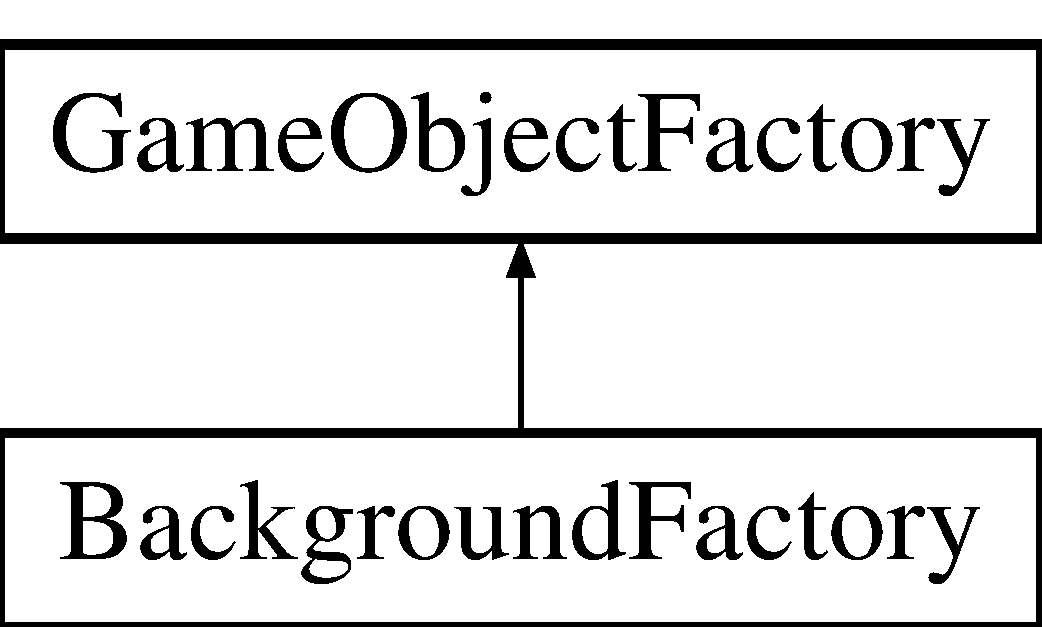
\includegraphics[height=2.000000cm]{d1/d41/class_background_factory}
\end{center}
\end{figure}
\subsection*{Public Member Functions}
\begin{DoxyCompactItemize}
\item 
\hyperlink{class_background_factory_acd0ab3d204fe6df9d2c32da4b8acc3fe}{Background\+Factory} (std\+::string background\+ID=\char`\"{}splash\+Screen\char`\"{})
\begin{DoxyCompactList}\small\item\em Costructs a \hyperlink{class_background_factory}{Background\+Factory} which creates the specific \hyperlink{class_splash_screen}{Splash\+Screen} defined by the background\+ID provided. \end{DoxyCompactList}\item 
virtual std\+::shared\+\_\+ptr$<$ \hyperlink{class_game_object}{Game\+Object} $>$ \hyperlink{class_background_factory_a17793b3ec704137388b70f53361691c3}{get\+Game\+Object} (const std\+::shared\+\_\+ptr$<$ \hyperlink{class_database_interface}{Database\+Interface} $>$ \&database) final
\begin{DoxyCompactList}\small\item\em Function call used to create a \hyperlink{class_game_object}{Game\+Object} used as a background. \end{DoxyCompactList}\item 
virtual \hyperlink{struct_game_object_data}{Game\+Object\+Data} \hyperlink{class_background_factory_aed13815bcb56568c4b465b5a531ee053}{get\+Object\+Data} (const std\+::shared\+\_\+ptr$<$ \hyperlink{class_database_interface}{Database\+Interface} $>$ \&database) final
\begin{DoxyCompactList}\small\item\em used to obtain the specific \hyperlink{struct_game_object_data}{Game\+Object\+Data} defined for the current factory \end{DoxyCompactList}\end{DoxyCompactItemize}
\subsection*{Private Attributes}
\begin{DoxyCompactItemize}
\item 
std\+::string \hyperlink{class_background_factory_a88dfa3ed001d4975bc8a76f5603d5017}{\+\_\+background\+ID}
\end{DoxyCompactItemize}


\subsection{Detailed Description}
\hyperlink{class_background_factory}{Background\+Factory} uses the template design pattern to create the various \hyperlink{class_splash_screen}{Splash\+Screen} objects used within the game. 

\subsection{Constructor \& Destructor Documentation}
\mbox{\Hypertarget{class_background_factory_acd0ab3d204fe6df9d2c32da4b8acc3fe}\label{class_background_factory_acd0ab3d204fe6df9d2c32da4b8acc3fe}} 
\index{Background\+Factory@{Background\+Factory}!Background\+Factory@{Background\+Factory}}
\index{Background\+Factory@{Background\+Factory}!Background\+Factory@{Background\+Factory}}
\subsubsection{\texorpdfstring{Background\+Factory()}{BackgroundFactory()}}
{\footnotesize\ttfamily Background\+Factory\+::\+Background\+Factory (\begin{DoxyParamCaption}\item[{std\+::string}]{background\+ID = {\ttfamily \char`\"{}splashScreen\char`\"{}} }\end{DoxyParamCaption})\hspace{0.3cm}{\ttfamily [inline]}}



Costructs a \hyperlink{class_background_factory}{Background\+Factory} which creates the specific \hyperlink{class_splash_screen}{Splash\+Screen} defined by the background\+ID provided. 


\begin{DoxyParams}{Parameters}
{\em background\+ID} & \\
\hline
\end{DoxyParams}


\subsection{Member Function Documentation}
\mbox{\Hypertarget{class_background_factory_a17793b3ec704137388b70f53361691c3}\label{class_background_factory_a17793b3ec704137388b70f53361691c3}} 
\index{Background\+Factory@{Background\+Factory}!get\+Game\+Object@{get\+Game\+Object}}
\index{get\+Game\+Object@{get\+Game\+Object}!Background\+Factory@{Background\+Factory}}
\subsubsection{\texorpdfstring{get\+Game\+Object()}{getGameObject()}}
{\footnotesize\ttfamily std\+::shared\+\_\+ptr$<$ \hyperlink{class_game_object}{Game\+Object} $>$ Background\+Factory\+::get\+Game\+Object (\begin{DoxyParamCaption}\item[{const std\+::shared\+\_\+ptr$<$ \hyperlink{class_database_interface}{Database\+Interface} $>$ \&}]{database }\end{DoxyParamCaption})\hspace{0.3cm}{\ttfamily [final]}, {\ttfamily [virtual]}}



Function call used to create a \hyperlink{class_game_object}{Game\+Object} used as a background. 


\begin{DoxyParams}{Parameters}
{\em database} & The specific \hyperlink{class_database_interface}{Database\+Interface} that contains the information about the Game\+Objects \\
\hline
\end{DoxyParams}
\begin{DoxyReturn}{Returns}
Returns a \hyperlink{class_game_object}{Game\+Object} with the specific graphic object for a specific background 
\end{DoxyReturn}


Reimplemented from \hyperlink{class_game_object_factory_a5b684a6e77fb82c041f1721eb07c553d}{Game\+Object\+Factory}.

\mbox{\Hypertarget{class_background_factory_aed13815bcb56568c4b465b5a531ee053}\label{class_background_factory_aed13815bcb56568c4b465b5a531ee053}} 
\index{Background\+Factory@{Background\+Factory}!get\+Object\+Data@{get\+Object\+Data}}
\index{get\+Object\+Data@{get\+Object\+Data}!Background\+Factory@{Background\+Factory}}
\subsubsection{\texorpdfstring{get\+Object\+Data()}{getObjectData()}}
{\footnotesize\ttfamily \hyperlink{struct_game_object_data}{Game\+Object\+Data} Background\+Factory\+::get\+Object\+Data (\begin{DoxyParamCaption}\item[{const std\+::shared\+\_\+ptr$<$ \hyperlink{class_database_interface}{Database\+Interface} $>$ \&}]{database }\end{DoxyParamCaption})\hspace{0.3cm}{\ttfamily [final]}, {\ttfamily [virtual]}}



used to obtain the specific \hyperlink{struct_game_object_data}{Game\+Object\+Data} defined for the current factory 


\begin{DoxyParams}{Parameters}
{\em database} & The specific \hyperlink{class_database_interface}{Database\+Interface} that contains the information about the Game\+Objects \\
\hline
\end{DoxyParams}
\begin{DoxyReturn}{Returns}
The \hyperlink{struct_game_object_data}{Game\+Object\+Data} required for the construction of the object 
\end{DoxyReturn}


Implements \hyperlink{class_game_object_factory_ae9358fbb3ef2d3b127320341760d3ff9}{Game\+Object\+Factory}.



\subsection{Member Data Documentation}
\mbox{\Hypertarget{class_background_factory_a88dfa3ed001d4975bc8a76f5603d5017}\label{class_background_factory_a88dfa3ed001d4975bc8a76f5603d5017}} 
\index{Background\+Factory@{Background\+Factory}!\+\_\+background\+ID@{\+\_\+background\+ID}}
\index{\+\_\+background\+ID@{\+\_\+background\+ID}!Background\+Factory@{Background\+Factory}}
\subsubsection{\texorpdfstring{\+\_\+background\+ID}{\_backgroundID}}
{\footnotesize\ttfamily std\+::string Background\+Factory\+::\+\_\+background\+ID\hspace{0.3cm}{\ttfamily [private]}}

The specific \hyperlink{class_splash_screen}{Splash\+Screen} Object that is created 

The documentation for this class was generated from the following files\+:\begin{DoxyCompactItemize}
\item 
C\+:/\+Users/\+Tim/\+Documents/\+Software\+Dev/\+Software\+Project/\+Project\+Files/game-\/source-\/code/\+Back\+End\+Systems/Background\+Factory.\+h\item 
C\+:/\+Users/\+Tim/\+Documents/\+Software\+Dev/\+Software\+Project/\+Project\+Files/game-\/source-\/code/\+Back\+End\+Systems/Background\+Factory.\+cpp\end{DoxyCompactItemize}

\hypertarget{class_basic_shoot}{}\section{Basic\+Shoot Class Reference}
\label{class_basic_shoot}\index{Basic\+Shoot@{Basic\+Shoot}}


Used to create a basic shoot component which creates a single projectile and shoots it in a straightline towards a target.  




{\ttfamily \#include $<$Basic\+Shoot.\+h$>$}

Inheritance diagram for Basic\+Shoot\+:\begin{figure}[H]
\begin{center}
\leavevmode
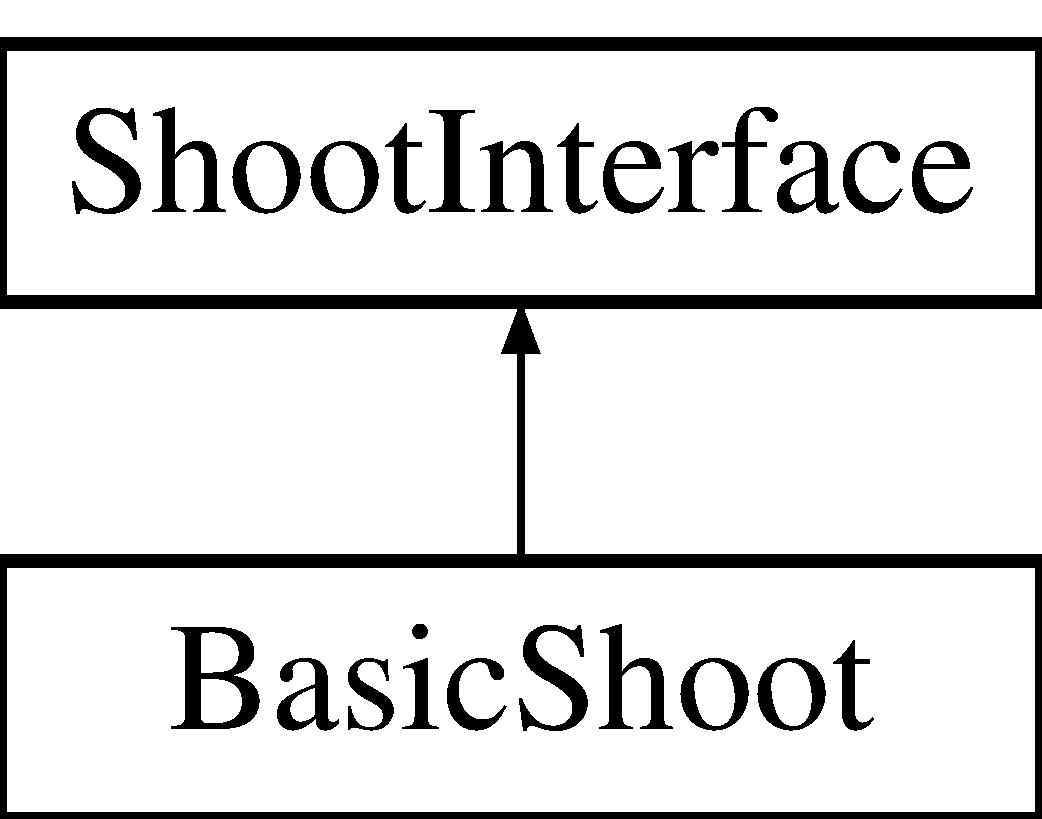
\includegraphics[height=2.000000cm]{d0/d31/class_basic_shoot}
\end{center}
\end{figure}
\subsection*{Public Member Functions}
\begin{DoxyCompactItemize}
\item 
\hyperlink{class_basic_shoot_a7594a4b840d698baa8d4a51027078727}{Basic\+Shoot} (Game\+Object\+Type projectile\+Type)
\begin{DoxyCompactList}\small\item\em Constructs the \hyperlink{class_basic_shoot}{Basic\+Shoot} Object used to create a projectile that fires in a straight line to a target. \end{DoxyCompactList}\item 
virtual void \hyperlink{class_basic_shoot_a8bed811408d1afa3ecf0454ae78f2303}{Shoot} (\hyperlink{class_vector2_d}{Vector2D} start\+Position, \hyperlink{class_vector2_d}{Vector2D} target, std\+::shared\+\_\+ptr$<$ \hyperlink{class_scene}{Scene} $>$ scene) override
\begin{DoxyCompactList}\small\item\em Shoots a \hyperlink{class_projectile}{Projectile} object in a way defined by the derived class, used as the main interface with the client. \end{DoxyCompactList}\end{DoxyCompactItemize}
\subsection*{Protected Member Functions}
\begin{DoxyCompactItemize}
\item 
virtual std\+::shared\+\_\+ptr$<$ \hyperlink{class_projectile}{Projectile} $>$ \hyperlink{class_basic_shoot_ab5058d147ca9d9cc4cc4210e9e092de5}{get\+Projectile} () override
\begin{DoxyCompactList}\small\item\em Overriden function used to get the projectile used by the \hyperlink{class_basic_shoot}{Basic\+Shoot} object. \end{DoxyCompactList}\end{DoxyCompactItemize}
\subsection*{Private Member Functions}
\begin{DoxyCompactItemize}
\item 
\hyperlink{class_vector2_d}{Vector2D} \hyperlink{class_basic_shoot_aafe1225544d200da3e0c084d33dac60a}{Calculate\+Shoot\+Direction} (\hyperlink{class_vector2_d}{Vector2D} start\+Position, \hyperlink{class_vector2_d}{Vector2D} target)
\begin{DoxyCompactList}\small\item\em Calculates the direction that the projectile from the start position to the target. \end{DoxyCompactList}\end{DoxyCompactItemize}
\subsection*{Private Attributes}
\begin{DoxyCompactItemize}
\item 
Game\+Object\+Type \hyperlink{class_basic_shoot_a3dfb89cab41f16d9bcb1e94f521978fe}{\+\_\+projectile\+Type}
\end{DoxyCompactItemize}


\subsection{Detailed Description}
Used to create a basic shoot component which creates a single projectile and shoots it in a straightline towards a target. 

\subsection{Constructor \& Destructor Documentation}
\mbox{\Hypertarget{class_basic_shoot_a7594a4b840d698baa8d4a51027078727}\label{class_basic_shoot_a7594a4b840d698baa8d4a51027078727}} 
\index{Basic\+Shoot@{Basic\+Shoot}!Basic\+Shoot@{Basic\+Shoot}}
\index{Basic\+Shoot@{Basic\+Shoot}!Basic\+Shoot@{Basic\+Shoot}}
\subsubsection{\texorpdfstring{Basic\+Shoot()}{BasicShoot()}}
{\footnotesize\ttfamily Basic\+Shoot\+::\+Basic\+Shoot (\begin{DoxyParamCaption}\item[{Game\+Object\+Type}]{projectile\+Type }\end{DoxyParamCaption})}



Constructs the \hyperlink{class_basic_shoot}{Basic\+Shoot} Object used to create a projectile that fires in a straight line to a target. 


\begin{DoxyParams}{Parameters}
{\em projectile\+Type} & The Game\+Object\+Type used to define the specific \hyperlink{class_projectile}{Projectile} that is created and shot \\
\hline
\end{DoxyParams}


\subsection{Member Function Documentation}
\mbox{\Hypertarget{class_basic_shoot_aafe1225544d200da3e0c084d33dac60a}\label{class_basic_shoot_aafe1225544d200da3e0c084d33dac60a}} 
\index{Basic\+Shoot@{Basic\+Shoot}!Calculate\+Shoot\+Direction@{Calculate\+Shoot\+Direction}}
\index{Calculate\+Shoot\+Direction@{Calculate\+Shoot\+Direction}!Basic\+Shoot@{Basic\+Shoot}}
\subsubsection{\texorpdfstring{Calculate\+Shoot\+Direction()}{CalculateShootDirection()}}
{\footnotesize\ttfamily \hyperlink{class_vector2_d}{Vector2D} Basic\+Shoot\+::\+Calculate\+Shoot\+Direction (\begin{DoxyParamCaption}\item[{\hyperlink{class_vector2_d}{Vector2D}}]{start\+Position,  }\item[{\hyperlink{class_vector2_d}{Vector2D}}]{target }\end{DoxyParamCaption})\hspace{0.3cm}{\ttfamily [private]}}



Calculates the direction that the projectile from the start position to the target. 


\begin{DoxyParams}{Parameters}
{\em start\+Position} & The starting position of the projectile \\
\hline
{\em target} & The target that the projectile needs to move towards \\
\hline
\end{DoxyParams}
\begin{DoxyReturn}{Returns}
Returns a \hyperlink{class_vector2_d}{Vector2D} that represents the unit direction from the start position to the target 
\end{DoxyReturn}
\mbox{\Hypertarget{class_basic_shoot_ab5058d147ca9d9cc4cc4210e9e092de5}\label{class_basic_shoot_ab5058d147ca9d9cc4cc4210e9e092de5}} 
\index{Basic\+Shoot@{Basic\+Shoot}!get\+Projectile@{get\+Projectile}}
\index{get\+Projectile@{get\+Projectile}!Basic\+Shoot@{Basic\+Shoot}}
\subsubsection{\texorpdfstring{get\+Projectile()}{getProjectile()}}
{\footnotesize\ttfamily std\+::shared\+\_\+ptr$<$ \hyperlink{class_projectile}{Projectile} $>$ Basic\+Shoot\+::get\+Projectile (\begin{DoxyParamCaption}{ }\end{DoxyParamCaption})\hspace{0.3cm}{\ttfamily [override]}, {\ttfamily [protected]}, {\ttfamily [virtual]}}



Overriden function used to get the projectile used by the \hyperlink{class_basic_shoot}{Basic\+Shoot} object. 

Uses the \hyperlink{class_repository}{Repository} to construct the specific projectile object that is defined by the \+\_\+projectile\+Type \begin{DoxyReturn}{Returns}
Returns the generated projectile that needs to be shot by the shoot component 
\end{DoxyReturn}


Implements \hyperlink{class_shoot_interface_ad274b0c66a0a42bf194b32b704c8bfea}{Shoot\+Interface}.

\mbox{\Hypertarget{class_basic_shoot_a8bed811408d1afa3ecf0454ae78f2303}\label{class_basic_shoot_a8bed811408d1afa3ecf0454ae78f2303}} 
\index{Basic\+Shoot@{Basic\+Shoot}!Shoot@{Shoot}}
\index{Shoot@{Shoot}!Basic\+Shoot@{Basic\+Shoot}}
\subsubsection{\texorpdfstring{Shoot()}{Shoot()}}
{\footnotesize\ttfamily void Basic\+Shoot\+::\+Shoot (\begin{DoxyParamCaption}\item[{\hyperlink{class_vector2_d}{Vector2D}}]{start\+Position,  }\item[{\hyperlink{class_vector2_d}{Vector2D}}]{target,  }\item[{std\+::shared\+\_\+ptr$<$ \hyperlink{class_scene}{Scene} $>$}]{scene }\end{DoxyParamCaption})\hspace{0.3cm}{\ttfamily [override]}, {\ttfamily [virtual]}}



Shoots a \hyperlink{class_projectile}{Projectile} object in a way defined by the derived class, used as the main interface with the client. 


\begin{DoxyParams}{Parameters}
{\em start\+Position} & The starting position of the \hyperlink{class_projectile}{Projectile} \\
\hline
{\em target} & The target that the projectile moves towards \\
\hline
{\em scene} & The scene that the projectile is instantiated into \\
\hline
\end{DoxyParams}


Implements \hyperlink{class_shoot_interface_a67205cc4e2fed90fa8c1ec93b30b864d}{Shoot\+Interface}.



\subsection{Member Data Documentation}
\mbox{\Hypertarget{class_basic_shoot_a3dfb89cab41f16d9bcb1e94f521978fe}\label{class_basic_shoot_a3dfb89cab41f16d9bcb1e94f521978fe}} 
\index{Basic\+Shoot@{Basic\+Shoot}!\+\_\+projectile\+Type@{\+\_\+projectile\+Type}}
\index{\+\_\+projectile\+Type@{\+\_\+projectile\+Type}!Basic\+Shoot@{Basic\+Shoot}}
\subsubsection{\texorpdfstring{\+\_\+projectile\+Type}{\_projectileType}}
{\footnotesize\ttfamily Game\+Object\+Type Basic\+Shoot\+::\+\_\+projectile\+Type\hspace{0.3cm}{\ttfamily [private]}}

The Game\+Object\+Type used to deferentiat the various projectiles that can be created 

The documentation for this class was generated from the following files\+:\begin{DoxyCompactItemize}
\item 
D\+:/\+Users/\+Tim-\/\+P\+C/\+Documents/\+Software\+\_\+\+I\+I/\+Project/\+Project\+Files/game-\/source-\/code/\+Front\+End\+Systems/Basic\+Shoot.\+h\item 
D\+:/\+Users/\+Tim-\/\+P\+C/\+Documents/\+Software\+\_\+\+I\+I/\+Project/\+Project\+Files/game-\/source-\/code/\+Front\+End\+Systems/Basic\+Shoot.\+cpp\end{DoxyCompactItemize}

\hypertarget{class_boundary}{}\section{Boundary Class Reference}
\label{class_boundary}\index{Boundary@{Boundary}}


\hyperlink{class_boundary}{Boundary} class used to represent a region of space centred around the origin, is able to determine if a specific point exists inside or outside of the bounds.  




{\ttfamily \#include $<$Boundary.\+h$>$}

\subsection*{Public Member Functions}
\begin{DoxyCompactItemize}
\item 
\hyperlink{class_boundary_a7c4c8db45b13dab630e4c6ed7a958e71}{Boundary} ()
\begin{DoxyCompactList}\small\item\em Default Constructor. \end{DoxyCompactList}\item 
\hyperlink{class_boundary_a1ebdbcf1f4bfc6c98ec89e0f15754a59}{Boundary} (double xbound, double ybound)
\begin{DoxyCompactList}\small\item\em Creates a boundary with the specified x and y bound. \end{DoxyCompactList}\item 
bool \hyperlink{class_boundary_a92d424b11ae1362dcb0b352c9c6aaed3}{Out\+Of\+Bounds} (const \hyperlink{class_vector2_d}{Vector2D} \&object\+Position) const
\begin{DoxyCompactList}\small\item\em Determines if a specific \hyperlink{class_vector2_d}{Vector2D} position is outside of the defined bounds. \end{DoxyCompactList}\item 
bool \hyperlink{class_boundary_ae307f83cb40ccaa89e37f58d007c4e6b}{inside\+Of\+Bounds} (const \hyperlink{class_vector2_d}{Vector2D} \&object\+Position) const
\begin{DoxyCompactList}\small\item\em Determines if a specific \hyperlink{class_vector2_d}{Vector2D} position is inside of the defined bounds. \end{DoxyCompactList}\end{DoxyCompactItemize}
\subsection*{Private Member Functions}
\begin{DoxyCompactItemize}
\item 
bool \hyperlink{class_boundary_a5063de08946b8303ddeff4c2b72e202e}{Checky\+Outof\+Bounds} (double y\+Pos) const
\begin{DoxyCompactList}\small\item\em Checks if the y position specified is within the y bounds. \end{DoxyCompactList}\item 
bool \hyperlink{class_boundary_a10d2d43b80364ce04cb22b90c9b54493}{Checkx\+Outof\+Bounds} (double x\+Pos) const
\begin{DoxyCompactList}\small\item\em Checks if the x position specified is within the x bounds. \end{DoxyCompactList}\end{DoxyCompactItemize}
\subsection*{Private Attributes}
\begin{DoxyCompactItemize}
\item 
double \hyperlink{class_boundary_a55685a68cc9b709898bdbe632d2dfeec}{\+\_\+x\+Bound}
\item 
double \hyperlink{class_boundary_a709e9e1f24faec6d4a35b50e6faffb8e}{\+\_\+y\+Bound}
\end{DoxyCompactItemize}


\subsection{Detailed Description}
\hyperlink{class_boundary}{Boundary} class used to represent a region of space centred around the origin, is able to determine if a specific point exists inside or outside of the bounds. 

\subsection{Constructor \& Destructor Documentation}
\mbox{\Hypertarget{class_boundary_a7c4c8db45b13dab630e4c6ed7a958e71}\label{class_boundary_a7c4c8db45b13dab630e4c6ed7a958e71}} 
\index{Boundary@{Boundary}!Boundary@{Boundary}}
\index{Boundary@{Boundary}!Boundary@{Boundary}}
\subsubsection{\texorpdfstring{Boundary()}{Boundary()}\hspace{0.1cm}{\footnotesize\ttfamily [1/2]}}
{\footnotesize\ttfamily Boundary\+::\+Boundary (\begin{DoxyParamCaption}{ }\end{DoxyParamCaption})}



Default Constructor. 

Creates the a boundary object with the current screen position as the default bounds \mbox{\Hypertarget{class_boundary_a1ebdbcf1f4bfc6c98ec89e0f15754a59}\label{class_boundary_a1ebdbcf1f4bfc6c98ec89e0f15754a59}} 
\index{Boundary@{Boundary}!Boundary@{Boundary}}
\index{Boundary@{Boundary}!Boundary@{Boundary}}
\subsubsection{\texorpdfstring{Boundary()}{Boundary()}\hspace{0.1cm}{\footnotesize\ttfamily [2/2]}}
{\footnotesize\ttfamily Boundary\+::\+Boundary (\begin{DoxyParamCaption}\item[{double}]{xbound,  }\item[{double}]{ybound }\end{DoxyParamCaption})}



Creates a boundary with the specified x and y bound. 


\begin{DoxyParams}{Parameters}
{\em xbound} & the distance of the boundary from the origin on the x axis \\
\hline
{\em ybound} & the distance of the boundary from the origin on the y axis \\
\hline
\end{DoxyParams}
\begin{DoxyReturn}{Returns}

\end{DoxyReturn}


\subsection{Member Function Documentation}
\mbox{\Hypertarget{class_boundary_a10d2d43b80364ce04cb22b90c9b54493}\label{class_boundary_a10d2d43b80364ce04cb22b90c9b54493}} 
\index{Boundary@{Boundary}!Checkx\+Outof\+Bounds@{Checkx\+Outof\+Bounds}}
\index{Checkx\+Outof\+Bounds@{Checkx\+Outof\+Bounds}!Boundary@{Boundary}}
\subsubsection{\texorpdfstring{Checkx\+Outof\+Bounds()}{CheckxOutofBounds()}}
{\footnotesize\ttfamily bool Boundary\+::\+Checkx\+Outof\+Bounds (\begin{DoxyParamCaption}\item[{double}]{x\+Pos }\end{DoxyParamCaption}) const\hspace{0.3cm}{\ttfamily [private]}}



Checks if the x position specified is within the x bounds. 


\begin{DoxyParams}{Parameters}
{\em x\+Pos} & The x position that is tested \\
\hline
\end{DoxyParams}
\begin{DoxyReturn}{Returns}
Returns a bool whether the x position specified is greater than or less than the x coordinate of the boundary 
\end{DoxyReturn}
\mbox{\Hypertarget{class_boundary_a5063de08946b8303ddeff4c2b72e202e}\label{class_boundary_a5063de08946b8303ddeff4c2b72e202e}} 
\index{Boundary@{Boundary}!Checky\+Outof\+Bounds@{Checky\+Outof\+Bounds}}
\index{Checky\+Outof\+Bounds@{Checky\+Outof\+Bounds}!Boundary@{Boundary}}
\subsubsection{\texorpdfstring{Checky\+Outof\+Bounds()}{CheckyOutofBounds()}}
{\footnotesize\ttfamily bool Boundary\+::\+Checky\+Outof\+Bounds (\begin{DoxyParamCaption}\item[{double}]{y\+Pos }\end{DoxyParamCaption}) const\hspace{0.3cm}{\ttfamily [private]}}



Checks if the y position specified is within the y bounds. 


\begin{DoxyParams}{Parameters}
{\em y\+Pos} & The y position that is tested \\
\hline
\end{DoxyParams}
\begin{DoxyReturn}{Returns}
Returns a bool whether the y position specified is greater than or less than the y coordinate of the boundary 
\end{DoxyReturn}
\mbox{\Hypertarget{class_boundary_ae307f83cb40ccaa89e37f58d007c4e6b}\label{class_boundary_ae307f83cb40ccaa89e37f58d007c4e6b}} 
\index{Boundary@{Boundary}!inside\+Of\+Bounds@{inside\+Of\+Bounds}}
\index{inside\+Of\+Bounds@{inside\+Of\+Bounds}!Boundary@{Boundary}}
\subsubsection{\texorpdfstring{inside\+Of\+Bounds()}{insideOfBounds()}}
{\footnotesize\ttfamily bool Boundary\+::inside\+Of\+Bounds (\begin{DoxyParamCaption}\item[{const \hyperlink{class_vector2_d}{Vector2D} \&}]{object\+Position }\end{DoxyParamCaption}) const}



Determines if a specific \hyperlink{class_vector2_d}{Vector2D} position is inside of the defined bounds. 


\begin{DoxyParams}{Parameters}
{\em object\+Position} & The specific position that is tested with the bounds \\
\hline
\end{DoxyParams}
\begin{DoxyReturn}{Returns}
Returns a bool whether the specified position is inside of the boundary 
\end{DoxyReturn}
\mbox{\Hypertarget{class_boundary_a92d424b11ae1362dcb0b352c9c6aaed3}\label{class_boundary_a92d424b11ae1362dcb0b352c9c6aaed3}} 
\index{Boundary@{Boundary}!Out\+Of\+Bounds@{Out\+Of\+Bounds}}
\index{Out\+Of\+Bounds@{Out\+Of\+Bounds}!Boundary@{Boundary}}
\subsubsection{\texorpdfstring{Out\+Of\+Bounds()}{OutOfBounds()}}
{\footnotesize\ttfamily bool Boundary\+::\+Out\+Of\+Bounds (\begin{DoxyParamCaption}\item[{const \hyperlink{class_vector2_d}{Vector2D} \&}]{object\+Position }\end{DoxyParamCaption}) const}



Determines if a specific \hyperlink{class_vector2_d}{Vector2D} position is outside of the defined bounds. 


\begin{DoxyParams}{Parameters}
{\em object\+Position} & The specific position that is tested with the bounds \\
\hline
\end{DoxyParams}
\begin{DoxyReturn}{Returns}
Returns a bool whether the specified position is outside of the boundary 
\end{DoxyReturn}


\subsection{Member Data Documentation}
\mbox{\Hypertarget{class_boundary_a55685a68cc9b709898bdbe632d2dfeec}\label{class_boundary_a55685a68cc9b709898bdbe632d2dfeec}} 
\index{Boundary@{Boundary}!\+\_\+x\+Bound@{\+\_\+x\+Bound}}
\index{\+\_\+x\+Bound@{\+\_\+x\+Bound}!Boundary@{Boundary}}
\subsubsection{\texorpdfstring{\+\_\+x\+Bound}{\_xBound}}
{\footnotesize\ttfamily double Boundary\+::\+\_\+x\+Bound\hspace{0.3cm}{\ttfamily [private]}}

The x value of the boundary specified \mbox{\Hypertarget{class_boundary_a709e9e1f24faec6d4a35b50e6faffb8e}\label{class_boundary_a709e9e1f24faec6d4a35b50e6faffb8e}} 
\index{Boundary@{Boundary}!\+\_\+y\+Bound@{\+\_\+y\+Bound}}
\index{\+\_\+y\+Bound@{\+\_\+y\+Bound}!Boundary@{Boundary}}
\subsubsection{\texorpdfstring{\+\_\+y\+Bound}{\_yBound}}
{\footnotesize\ttfamily double Boundary\+::\+\_\+y\+Bound\hspace{0.3cm}{\ttfamily [private]}}

The y value of the boundary specified 

The documentation for this class was generated from the following files\+:\begin{DoxyCompactItemize}
\item 
C\+:/\+Users/\+Tim/\+Documents/\+Software\+Dev/\+Software\+Project/\+Project\+Files/game-\/source-\/code/\+Front\+End\+Systems/Boundary.\+h\item 
C\+:/\+Users/\+Tim/\+Documents/\+Software\+Dev/\+Software\+Project/\+Project\+Files/game-\/source-\/code/\+Front\+End\+Systems/Boundary.\+cpp\end{DoxyCompactItemize}

\hypertarget{class_collision_detection}{}\section{Collision\+Detection Class Reference}
\label{class_collision_detection}\index{Collision\+Detection@{Collision\+Detection}}


Determines when Physics\+Objects have collided with each other.  




{\ttfamily \#include $<$Collision\+Detection.\+h$>$}

\subsection*{Public Member Functions}
\begin{DoxyCompactItemize}
\item 
\hyperlink{class_collision_detection_a2f88d35b750b96c0da3b09460d8f02bd}{Collision\+Detection} (sf\+::\+Render\+Window $\ast$disp\+Window)
\begin{DoxyCompactList}\small\item\em Constructs the \hyperlink{class_collision_detection}{Collision\+Detection} object with the specific Render\+Window that is required to create a \hyperlink{class_collision_detection}{Collision\+Detection} loop. \end{DoxyCompactList}\item 
\mbox{\Hypertarget{class_collision_detection_a6fcb59ac9cafa41ba26912f72c1bf990}\label{class_collision_detection_a6fcb59ac9cafa41ba26912f72c1bf990}} 
void \hyperlink{class_collision_detection_a6fcb59ac9cafa41ba26912f72c1bf990}{Initialize\+Collision\+Thread} ()
\begin{DoxyCompactList}\small\item\em Initialises the \hyperlink{class_collision_detection}{Collision\+Detection} thread. \end{DoxyCompactList}\end{DoxyCompactItemize}
\subsection*{Private Member Functions}
\begin{DoxyCompactItemize}
\item 
\mbox{\Hypertarget{class_collision_detection_a1eda3727a959c4aa24fad3ef46a7b530}\label{class_collision_detection_a1eda3727a959c4aa24fad3ef46a7b530}} 
void \hyperlink{class_collision_detection_a1eda3727a959c4aa24fad3ef46a7b530}{run\+Collision\+Thread} ()
\begin{DoxyCompactList}\small\item\em Contains the Collision Detection loop, checks for collisions on each iteration of the loop. \end{DoxyCompactList}\item 
void \hyperlink{class_collision_detection_a9b39c9264288db71452ce2f66a79c4f1}{check\+Collisions} ()
\begin{DoxyCompactList}\small\item\em Loops through each \hyperlink{class_game_object}{Game\+Object} and determines if it has collided with a different one. \end{DoxyCompactList}\item 
void \hyperlink{class_collision_detection_a5c7daf7f877c7f9418d36944c4728b75}{check\+Objects} (std\+::shared\+\_\+ptr$<$ \hyperlink{class_game_object}{Game\+Object} $>$ game\+Obj1, std\+::shared\+\_\+ptr$<$ \hyperlink{class_game_object}{Game\+Object} $>$ game\+Obj2)
\begin{DoxyCompactList}\small\item\em Checks if the two Physics\+Objects have collided with each other by dynamically casting the provided Game\+Objects. \end{DoxyCompactList}\end{DoxyCompactItemize}
\subsection*{Private Attributes}
\begin{DoxyCompactItemize}
\item 
sf\+::\+Render\+Window $\ast$ \hyperlink{class_collision_detection_a7a894b4bc38b6987d4cf8135df01d83b}{\+\_\+dispwindow\+\_\+ptr}
\end{DoxyCompactItemize}


\subsection{Detailed Description}
Determines when Physics\+Objects have collided with each other. 

Runs in a seperate thread and copies the list of Game\+Objects stored within the \hyperlink{class_scene}{Scene} 

\subsection{Constructor \& Destructor Documentation}
\mbox{\Hypertarget{class_collision_detection_a2f88d35b750b96c0da3b09460d8f02bd}\label{class_collision_detection_a2f88d35b750b96c0da3b09460d8f02bd}} 
\index{Collision\+Detection@{Collision\+Detection}!Collision\+Detection@{Collision\+Detection}}
\index{Collision\+Detection@{Collision\+Detection}!Collision\+Detection@{Collision\+Detection}}
\subsubsection{\texorpdfstring{Collision\+Detection()}{CollisionDetection()}}
{\footnotesize\ttfamily Collision\+Detection\+::\+Collision\+Detection (\begin{DoxyParamCaption}\item[{sf\+::\+Render\+Window $\ast$}]{disp\+Window }\end{DoxyParamCaption})}



Constructs the \hyperlink{class_collision_detection}{Collision\+Detection} object with the specific Render\+Window that is required to create a \hyperlink{class_collision_detection}{Collision\+Detection} loop. 


\begin{DoxyParams}{Parameters}
{\em disp\+Window} & The Render\+Window that is used for the game loop \\
\hline
\end{DoxyParams}


\subsection{Member Function Documentation}
\mbox{\Hypertarget{class_collision_detection_a9b39c9264288db71452ce2f66a79c4f1}\label{class_collision_detection_a9b39c9264288db71452ce2f66a79c4f1}} 
\index{Collision\+Detection@{Collision\+Detection}!check\+Collisions@{check\+Collisions}}
\index{check\+Collisions@{check\+Collisions}!Collision\+Detection@{Collision\+Detection}}
\subsubsection{\texorpdfstring{check\+Collisions()}{checkCollisions()}}
{\footnotesize\ttfamily void Collision\+Detection\+::check\+Collisions (\begin{DoxyParamCaption}{ }\end{DoxyParamCaption})\hspace{0.3cm}{\ttfamily [private]}}



Loops through each \hyperlink{class_game_object}{Game\+Object} and determines if it has collided with a different one. 

It is necesary to iterate through each element and compare it with every other element, each coparison only needs to be done once. This is achieved by starting from the first element (assuming it is the most left element) it compares itself to all elements of the container not including itself. \mbox{\Hypertarget{class_collision_detection_a5c7daf7f877c7f9418d36944c4728b75}\label{class_collision_detection_a5c7daf7f877c7f9418d36944c4728b75}} 
\index{Collision\+Detection@{Collision\+Detection}!check\+Objects@{check\+Objects}}
\index{check\+Objects@{check\+Objects}!Collision\+Detection@{Collision\+Detection}}
\subsubsection{\texorpdfstring{check\+Objects()}{checkObjects()}}
{\footnotesize\ttfamily void Collision\+Detection\+::check\+Objects (\begin{DoxyParamCaption}\item[{std\+::shared\+\_\+ptr$<$ \hyperlink{class_game_object}{Game\+Object} $>$}]{game\+Obj1,  }\item[{std\+::shared\+\_\+ptr$<$ \hyperlink{class_game_object}{Game\+Object} $>$}]{game\+Obj2 }\end{DoxyParamCaption})\hspace{0.3cm}{\ttfamily [private]}}



Checks if the two Physics\+Objects have collided with each other by dynamically casting the provided Game\+Objects. 


\begin{DoxyParams}{Parameters}
{\em game\+Obj1} & primary \hyperlink{class_game_object}{Game\+Object}, if a collision has occured collision\+Occured is called \\
\hline
{\em game\+Obj2} & secondary \hyperlink{class_game_object}{Game\+Object}, used to check if collision has occure with primary \hyperlink{class_game_object}{Game\+Object} \\
\hline
\end{DoxyParams}


\subsection{Member Data Documentation}
\mbox{\Hypertarget{class_collision_detection_a7a894b4bc38b6987d4cf8135df01d83b}\label{class_collision_detection_a7a894b4bc38b6987d4cf8135df01d83b}} 
\index{Collision\+Detection@{Collision\+Detection}!\+\_\+dispwindow\+\_\+ptr@{\+\_\+dispwindow\+\_\+ptr}}
\index{\+\_\+dispwindow\+\_\+ptr@{\+\_\+dispwindow\+\_\+ptr}!Collision\+Detection@{Collision\+Detection}}
\subsubsection{\texorpdfstring{\+\_\+dispwindow\+\_\+ptr}{\_dispwindow\_ptr}}
{\footnotesize\ttfamily sf\+::\+Render\+Window$\ast$ Collision\+Detection\+::\+\_\+dispwindow\+\_\+ptr\hspace{0.3cm}{\ttfamily [private]}}

pointer to the Render\+Window used for the game 

The documentation for this class was generated from the following files\+:\begin{DoxyCompactItemize}
\item 
D\+:/\+Users/\+Tim-\/\+P\+C/\+Documents/\+Software\+\_\+\+I\+I/\+Project/\+Project\+Files/game-\/source-\/code/\+Back\+End\+Systems/Collision\+Detection.\+h\item 
D\+:/\+Users/\+Tim-\/\+P\+C/\+Documents/\+Software\+\_\+\+I\+I/\+Project/\+Project\+Files/game-\/source-\/code/\+Back\+End\+Systems/Collision\+Detection.\+cpp\end{DoxyCompactItemize}

\hypertarget{class_data_already_exists_in_database}{}\section{Data\+Already\+Exists\+In\+Database Class Reference}
\label{class_data_already_exists_in_database}\index{Data\+Already\+Exists\+In\+Database@{Data\+Already\+Exists\+In\+Database}}


Exception thrown if information that exists in the database is overwritten.  




{\ttfamily \#include $<$Run\+Time\+Database.\+h$>$}



\subsection{Detailed Description}
Exception thrown if information that exists in the database is overwritten. 

The documentation for this class was generated from the following file\+:\begin{DoxyCompactItemize}
\item 
D\+:/\+Users/\+Tim-\/\+P\+C/\+Documents/\+Software\+\_\+\+I\+I/\+Project/\+Project\+Files/game-\/source-\/code/\+Back\+End\+Systems/Run\+Time\+Database.\+h\end{DoxyCompactItemize}

\hypertarget{class_database_interface}{}\section{Database\+Interface Class Reference}
\label{class_database_interface}\index{Database\+Interface@{Database\+Interface}}


Defines the interface necessary for any Database object implementations used to store information about the various Game\+Objects and the game state.  




{\ttfamily \#include $<$Database\+Interface.\+h$>$}

Inheritance diagram for Database\+Interface\+:\begin{figure}[H]
\begin{center}
\leavevmode
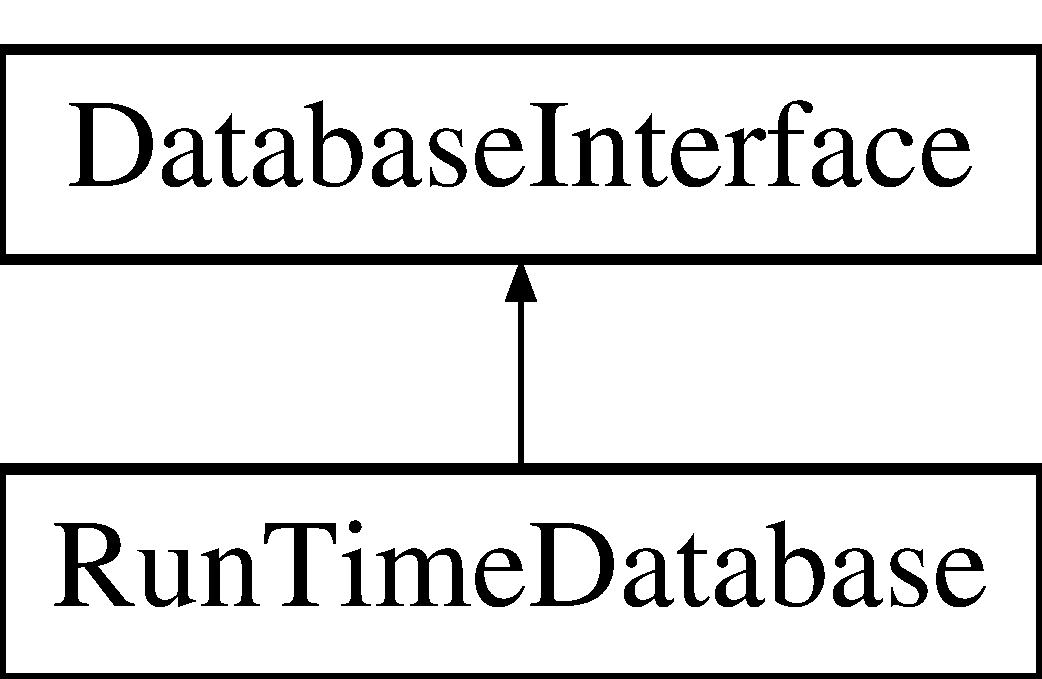
\includegraphics[height=2.000000cm]{d1/dff/class_database_interface}
\end{center}
\end{figure}
\subsection*{Public Member Functions}
\begin{DoxyCompactItemize}
\item 
virtual \hyperlink{struct_game_object_data}{Game\+Object\+Data} \hyperlink{class_database_interface_a515afa17b15a4b111ebc1a43e1d0218e}{get\+Game\+Object\+Data} (std\+::string ID)=0
\begin{DoxyCompactList}\small\item\em Used to obtain the various data that relates to the different Game\+Objects used inside the game. \end{DoxyCompactList}\item 
virtual \hyperlink{struct_game_state_data}{Game\+State\+Data} \hyperlink{class_database_interface_a5972ccdce7669da4eef8ab82c69fe073}{get\+Game\+State\+Data} ()=0
\begin{DoxyCompactList}\small\item\em Gets the data about the current state of the game. \end{DoxyCompactList}\item 
virtual void \hyperlink{class_database_interface_ae1914371cb425f71ba750f57f968b491}{set\+Game\+Object\+Data} (std\+::string ID, \hyperlink{struct_game_object_data}{Game\+Object\+Data} game\+Object\+Data)=0
\begin{DoxyCompactList}\small\item\em Sets the object data at the corresponding ID provided into the database. \end{DoxyCompactList}\item 
virtual void \hyperlink{class_database_interface_a0b2f4402583b6ab31c70c713d72ceede}{set\+Game\+State\+Data} (\hyperlink{struct_game_state_data}{Game\+State\+Data} game\+State\+Data)=0
\begin{DoxyCompactList}\small\item\em Sets the \hyperlink{struct_game_state_data}{Game\+State\+Data} inside of the database. \end{DoxyCompactList}\end{DoxyCompactItemize}


\subsection{Detailed Description}
Defines the interface necessary for any Database object implementations used to store information about the various Game\+Objects and the game state. 

\subsection{Member Function Documentation}
\mbox{\Hypertarget{class_database_interface_a515afa17b15a4b111ebc1a43e1d0218e}\label{class_database_interface_a515afa17b15a4b111ebc1a43e1d0218e}} 
\index{Database\+Interface@{Database\+Interface}!get\+Game\+Object\+Data@{get\+Game\+Object\+Data}}
\index{get\+Game\+Object\+Data@{get\+Game\+Object\+Data}!Database\+Interface@{Database\+Interface}}
\subsubsection{\texorpdfstring{get\+Game\+Object\+Data()}{getGameObjectData()}}
{\footnotesize\ttfamily virtual \hyperlink{struct_game_object_data}{Game\+Object\+Data} Database\+Interface\+::get\+Game\+Object\+Data (\begin{DoxyParamCaption}\item[{std\+::string}]{ID }\end{DoxyParamCaption})\hspace{0.3cm}{\ttfamily [pure virtual]}}



Used to obtain the various data that relates to the different Game\+Objects used inside the game. 


\begin{DoxyParams}{Parameters}
{\em ID} & The speciic ID required to return the correct object data \\
\hline
\end{DoxyParams}
\begin{DoxyReturn}{Returns}
Returns the \hyperlink{struct_game_object_data}{Game\+Object\+Data} relating to the object defined by the ID 
\end{DoxyReturn}


Implemented in \hyperlink{class_run_time_database_aabe246e23f6f8ded2c3b61fcfa396f2a}{Run\+Time\+Database}.

\mbox{\Hypertarget{class_database_interface_a5972ccdce7669da4eef8ab82c69fe073}\label{class_database_interface_a5972ccdce7669da4eef8ab82c69fe073}} 
\index{Database\+Interface@{Database\+Interface}!get\+Game\+State\+Data@{get\+Game\+State\+Data}}
\index{get\+Game\+State\+Data@{get\+Game\+State\+Data}!Database\+Interface@{Database\+Interface}}
\subsubsection{\texorpdfstring{get\+Game\+State\+Data()}{getGameStateData()}}
{\footnotesize\ttfamily virtual \hyperlink{struct_game_state_data}{Game\+State\+Data} Database\+Interface\+::get\+Game\+State\+Data (\begin{DoxyParamCaption}{ }\end{DoxyParamCaption})\hspace{0.3cm}{\ttfamily [pure virtual]}}



Gets the data about the current state of the game. 

\begin{DoxyReturn}{Returns}
Returns the \hyperlink{struct_game_state_data}{Game\+State\+Data} which relates to the game, including the game screen size and name 
\end{DoxyReturn}


Implemented in \hyperlink{class_run_time_database_a15d6105d3d772f604c42813e50ba4ee3}{Run\+Time\+Database}.

\mbox{\Hypertarget{class_database_interface_ae1914371cb425f71ba750f57f968b491}\label{class_database_interface_ae1914371cb425f71ba750f57f968b491}} 
\index{Database\+Interface@{Database\+Interface}!set\+Game\+Object\+Data@{set\+Game\+Object\+Data}}
\index{set\+Game\+Object\+Data@{set\+Game\+Object\+Data}!Database\+Interface@{Database\+Interface}}
\subsubsection{\texorpdfstring{set\+Game\+Object\+Data()}{setGameObjectData()}}
{\footnotesize\ttfamily virtual void Database\+Interface\+::set\+Game\+Object\+Data (\begin{DoxyParamCaption}\item[{std\+::string}]{ID,  }\item[{\hyperlink{struct_game_object_data}{Game\+Object\+Data}}]{game\+Object\+Data }\end{DoxyParamCaption})\hspace{0.3cm}{\ttfamily [pure virtual]}}



Sets the object data at the corresponding ID provided into the database. 


\begin{DoxyParams}{Parameters}
{\em ID} & The ID of the object that neeeds to be set within the database \\
\hline
{\em game\+Object\+Data} & The \hyperlink{struct_game_object_data}{Game\+Object\+Data} stored \\
\hline
\end{DoxyParams}


Implemented in \hyperlink{class_run_time_database_a9d2c5c2f1eb4dc728d69b9c5dbd1c22d}{Run\+Time\+Database}.

\mbox{\Hypertarget{class_database_interface_a0b2f4402583b6ab31c70c713d72ceede}\label{class_database_interface_a0b2f4402583b6ab31c70c713d72ceede}} 
\index{Database\+Interface@{Database\+Interface}!set\+Game\+State\+Data@{set\+Game\+State\+Data}}
\index{set\+Game\+State\+Data@{set\+Game\+State\+Data}!Database\+Interface@{Database\+Interface}}
\subsubsection{\texorpdfstring{set\+Game\+State\+Data()}{setGameStateData()}}
{\footnotesize\ttfamily virtual void Database\+Interface\+::set\+Game\+State\+Data (\begin{DoxyParamCaption}\item[{\hyperlink{struct_game_state_data}{Game\+State\+Data}}]{game\+State\+Data }\end{DoxyParamCaption})\hspace{0.3cm}{\ttfamily [pure virtual]}}



Sets the \hyperlink{struct_game_state_data}{Game\+State\+Data} inside of the database. 


\begin{DoxyParams}{Parameters}
{\em game\+State\+Data} & The specific \hyperlink{struct_game_state_data}{Game\+State\+Data} stored within the database \\
\hline
\end{DoxyParams}


Implemented in \hyperlink{class_run_time_database_af18f09a5166adc6ab075034e272e9c8d}{Run\+Time\+Database}.



The documentation for this class was generated from the following file\+:\begin{DoxyCompactItemize}
\item 
D\+:/\+Users/\+Tim-\/\+P\+C/\+Documents/\+Software\+\_\+\+I\+I/\+Project/\+Project\+Files/game-\/source-\/code/\+Back\+End\+Systems/Database\+Interface.\+h\end{DoxyCompactItemize}

\hypertarget{class_data_doesnt_exist_in_database}{}\section{Data\+Doesnt\+Exist\+In\+Database Class Reference}
\label{class_data_doesnt_exist_in_database}\index{Data\+Doesnt\+Exist\+In\+Database@{Data\+Doesnt\+Exist\+In\+Database}}


Exception thrown if information is accessed that doesnt exist in the database.  




{\ttfamily \#include $<$Run\+Time\+Database.\+h$>$}



\subsection{Detailed Description}
Exception thrown if information is accessed that doesnt exist in the database. 

The documentation for this class was generated from the following file\+:\begin{DoxyCompactItemize}
\item 
D\+:/\+Users/\+Tim-\/\+P\+C/\+Documents/\+Software\+\_\+\+I\+I/\+Project/\+Project\+Files/game-\/source-\/code/\+Back\+End\+Systems/Run\+Time\+Database.\+h\end{DoxyCompactItemize}

\hypertarget{class_data_mapper}{}\section{Data\+Mapper Class Reference}
\label{class_data_mapper}\index{Data\+Mapper@{Data\+Mapper}}


\hyperlink{class_data_mapper}{Data\+Mapper} is responsible for mapping data recieved from the \hyperlink{class_read_from_file}{Read\+From\+File} object into usable datatypes and interfacing with the desired datatbase to update the information in it.  




{\ttfamily \#include $<$Datamapper.\+h$>$}

Inheritance diagram for Data\+Mapper\+:\begin{figure}[H]
\begin{center}
\leavevmode
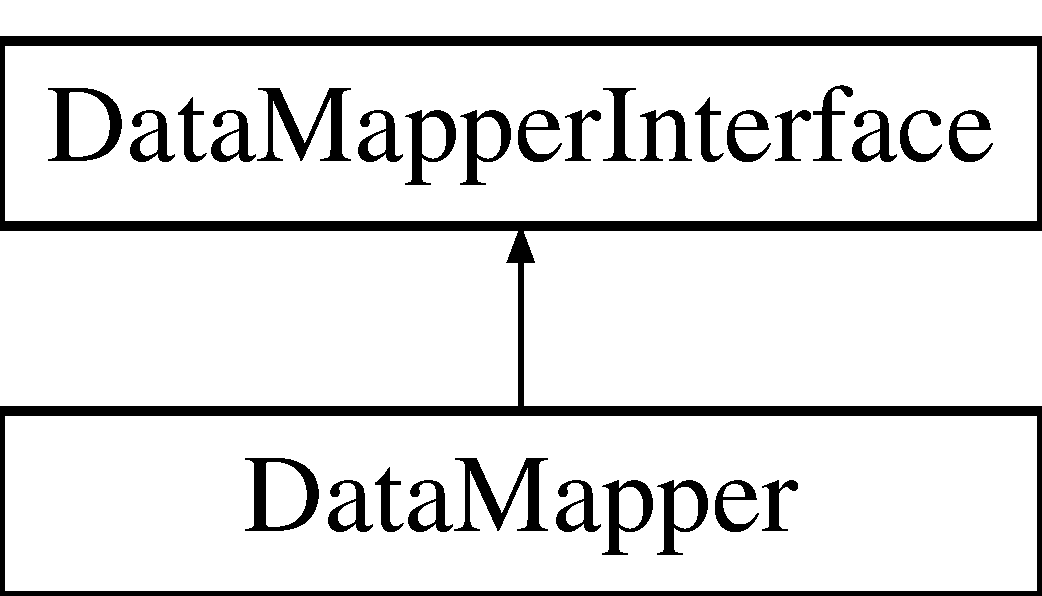
\includegraphics[height=2.000000cm]{dd/da0/class_data_mapper}
\end{center}
\end{figure}
\subsection*{Public Member Functions}
\begin{DoxyCompactItemize}
\item 
\hyperlink{class_data_mapper_a4603cf7c03ad31b454669ad61e64919f}{Data\+Mapper} (std\+::string gameobject\+\_\+datafile, std\+::string gamestate\+\_\+datafile)
\begin{DoxyCompactList}\small\item\em Constructs the \hyperlink{class_data_mapper}{Data\+Mapper} Object with two strings that represent the data files of the game. \end{DoxyCompactList}\item 
virtual void \hyperlink{class_data_mapper_ade3e27146120b3cb74d556e8b9e48526}{Update\+Game\+Time\+Database} (std\+::shared\+\_\+ptr$<$ \hyperlink{class_database_interface}{Database\+Interface} $>$ database) override
\begin{DoxyCompactList}\small\item\em Updates the the provided database with information stored in the datafiles provided. \end{DoxyCompactList}\end{DoxyCompactItemize}
\subsection*{Private Member Functions}
\begin{DoxyCompactItemize}
\item 
std\+::string \hyperlink{class_data_mapper_a46e3c795a3ec96a58dd1006079b0938d}{Get\+I\+D\+From\+String} (const std\+::string \&I\+D\+\_\+\+Line)
\begin{DoxyCompactList}\small\item\em Gets the ID of the object frm the string provided used as the key to store the information in the \hyperlink{class_database_interface}{Database\+Interface}. \end{DoxyCompactList}\item 
\hyperlink{struct_game_object_data}{Game\+Object\+Data} \hyperlink{class_data_mapper_a69d2e0ba874a2e3b0dd9752c1c72db34}{get\+Object\+Data\+From\+String} (const std\+::string \&Data\+Line)
\begin{DoxyCompactList}\small\item\em Converts and Constructs the \hyperlink{struct_game_object_data}{Game\+Object\+Data} from the string provided. \end{DoxyCompactList}\item 
std\+::vector$<$ std\+::string $>$ \hyperlink{class_data_mapper_a296af9345fd16e4397251efef8726a74}{Split\+Game\+Object\+Data\+String} (const std\+::string \&Data\+Line)
\begin{DoxyCompactList}\small\item\em Splits the string up into a vector of multiple strings seperated by spaces. \end{DoxyCompactList}\item 
void \hyperlink{class_data_mapper_af92f7728727500d39ff4aa1d6ca2b81b}{Update\+Game\+Object\+Database\+Info} (std\+::shared\+\_\+ptr$<$ \hyperlink{class_database_interface}{Database\+Interface} $>$ database)
\begin{DoxyCompactList}\small\item\em Updates the \hyperlink{struct_game_object_data}{Game\+Object\+Data} of the database. \end{DoxyCompactList}\item 
void \hyperlink{class_data_mapper_aefb6246f9bf9fc9974cd52a1b46d165e}{Update\+Game\+State\+Database\+Info} (std\+::shared\+\_\+ptr$<$ \hyperlink{class_database_interface}{Database\+Interface} $>$ database)
\begin{DoxyCompactList}\small\item\em Updates the Game\+State data of the database. \end{DoxyCompactList}\end{DoxyCompactItemize}
\subsection*{Private Attributes}
\begin{DoxyCompactItemize}
\item 
std\+::string \hyperlink{class_data_mapper_a7906ac7e6e95631428095246fcdefecb}{\+\_\+gameobject\+\_\+datafile}
\item 
std\+::string \hyperlink{class_data_mapper_ad64f65ef0ca4a3ed5e0ded4318ee3357}{\+\_\+gamestate\+\_\+datafile}
\end{DoxyCompactItemize}


\subsection{Detailed Description}
\hyperlink{class_data_mapper}{Data\+Mapper} is responsible for mapping data recieved from the \hyperlink{class_read_from_file}{Read\+From\+File} object into usable datatypes and interfacing with the desired datatbase to update the information in it. 

\subsection{Constructor \& Destructor Documentation}
\mbox{\Hypertarget{class_data_mapper_a4603cf7c03ad31b454669ad61e64919f}\label{class_data_mapper_a4603cf7c03ad31b454669ad61e64919f}} 
\index{Data\+Mapper@{Data\+Mapper}!Data\+Mapper@{Data\+Mapper}}
\index{Data\+Mapper@{Data\+Mapper}!Data\+Mapper@{Data\+Mapper}}
\subsubsection{\texorpdfstring{Data\+Mapper()}{DataMapper()}}
{\footnotesize\ttfamily Data\+Mapper\+::\+Data\+Mapper (\begin{DoxyParamCaption}\item[{std\+::string}]{gameobject\+\_\+datafile,  }\item[{std\+::string}]{gamestate\+\_\+datafile }\end{DoxyParamCaption})}



Constructs the \hyperlink{class_data_mapper}{Data\+Mapper} Object with two strings that represent the data files of the game. 


\begin{DoxyParams}{Parameters}
{\em gameobject\+\_\+datafile} & The datafile that contains the information about the various Game\+Objects of the game \\
\hline
{\em gamestate\+\_\+datafile} & The datafile that contains the information about the state of the game, ie screen size \\
\hline
\end{DoxyParams}


\subsection{Member Function Documentation}
\mbox{\Hypertarget{class_data_mapper_a46e3c795a3ec96a58dd1006079b0938d}\label{class_data_mapper_a46e3c795a3ec96a58dd1006079b0938d}} 
\index{Data\+Mapper@{Data\+Mapper}!Get\+I\+D\+From\+String@{Get\+I\+D\+From\+String}}
\index{Get\+I\+D\+From\+String@{Get\+I\+D\+From\+String}!Data\+Mapper@{Data\+Mapper}}
\subsubsection{\texorpdfstring{Get\+I\+D\+From\+String()}{GetIDFromString()}}
{\footnotesize\ttfamily std\+::string Data\+Mapper\+::\+Get\+I\+D\+From\+String (\begin{DoxyParamCaption}\item[{const std\+::string \&}]{I\+D\+\_\+\+Line }\end{DoxyParamCaption})\hspace{0.3cm}{\ttfamily [private]}}



Gets the ID of the object frm the string provided used as the key to store the information in the \hyperlink{class_database_interface}{Database\+Interface}. 


\begin{DoxyParams}{Parameters}
{\em I\+D\+\_\+\+Line} & The line obtained from the text file that contains the ID -\/ assumes the correct format is used within the text file \\
\hline
\end{DoxyParams}
\begin{DoxyReturn}{Returns}
returns the ID of the object obtained from the string 
\end{DoxyReturn}
\mbox{\Hypertarget{class_data_mapper_a69d2e0ba874a2e3b0dd9752c1c72db34}\label{class_data_mapper_a69d2e0ba874a2e3b0dd9752c1c72db34}} 
\index{Data\+Mapper@{Data\+Mapper}!get\+Object\+Data\+From\+String@{get\+Object\+Data\+From\+String}}
\index{get\+Object\+Data\+From\+String@{get\+Object\+Data\+From\+String}!Data\+Mapper@{Data\+Mapper}}
\subsubsection{\texorpdfstring{get\+Object\+Data\+From\+String()}{getObjectDataFromString()}}
{\footnotesize\ttfamily \hyperlink{struct_game_object_data}{Game\+Object\+Data} Data\+Mapper\+::get\+Object\+Data\+From\+String (\begin{DoxyParamCaption}\item[{const std\+::string \&}]{Data\+Line }\end{DoxyParamCaption})\hspace{0.3cm}{\ttfamily [private]}}



Converts and Constructs the \hyperlink{struct_game_object_data}{Game\+Object\+Data} from the string provided. 


\begin{DoxyParams}{Parameters}
{\em Data\+Line} & a string containing the various object information \\
\hline
\end{DoxyParams}
\begin{DoxyReturn}{Returns}
Returns a \hyperlink{struct_game_object_data}{Game\+Object\+Data} constructed from the information provided by the string of data 
\end{DoxyReturn}
\mbox{\Hypertarget{class_data_mapper_a296af9345fd16e4397251efef8726a74}\label{class_data_mapper_a296af9345fd16e4397251efef8726a74}} 
\index{Data\+Mapper@{Data\+Mapper}!Split\+Game\+Object\+Data\+String@{Split\+Game\+Object\+Data\+String}}
\index{Split\+Game\+Object\+Data\+String@{Split\+Game\+Object\+Data\+String}!Data\+Mapper@{Data\+Mapper}}
\subsubsection{\texorpdfstring{Split\+Game\+Object\+Data\+String()}{SplitGameObjectDataString()}}
{\footnotesize\ttfamily std\+::vector$<$ std\+::string $>$ Data\+Mapper\+::\+Split\+Game\+Object\+Data\+String (\begin{DoxyParamCaption}\item[{const std\+::string \&}]{Data\+Line }\end{DoxyParamCaption})\hspace{0.3cm}{\ttfamily [private]}}



Splits the string up into a vector of multiple strings seperated by spaces. 


\begin{DoxyParams}{Parameters}
{\em Data\+Line} & a string containing the various object information \\
\hline
\end{DoxyParams}
\begin{DoxyReturn}{Returns}
Returns a vector of strings each representing a specific element of the \hyperlink{struct_game_object_data}{Game\+Object\+Data} 
\end{DoxyReturn}
\mbox{\Hypertarget{class_data_mapper_af92f7728727500d39ff4aa1d6ca2b81b}\label{class_data_mapper_af92f7728727500d39ff4aa1d6ca2b81b}} 
\index{Data\+Mapper@{Data\+Mapper}!Update\+Game\+Object\+Database\+Info@{Update\+Game\+Object\+Database\+Info}}
\index{Update\+Game\+Object\+Database\+Info@{Update\+Game\+Object\+Database\+Info}!Data\+Mapper@{Data\+Mapper}}
\subsubsection{\texorpdfstring{Update\+Game\+Object\+Database\+Info()}{UpdateGameObjectDatabaseInfo()}}
{\footnotesize\ttfamily void Data\+Mapper\+::\+Update\+Game\+Object\+Database\+Info (\begin{DoxyParamCaption}\item[{std\+::shared\+\_\+ptr$<$ \hyperlink{class_database_interface}{Database\+Interface} $>$}]{database }\end{DoxyParamCaption})\hspace{0.3cm}{\ttfamily [private]}}



Updates the \hyperlink{struct_game_object_data}{Game\+Object\+Data} of the database. 


\begin{DoxyParams}{Parameters}
{\em database} & the \hyperlink{class_database_interface}{Database\+Interface} that is updated \\
\hline
\end{DoxyParams}
\mbox{\Hypertarget{class_data_mapper_aefb6246f9bf9fc9974cd52a1b46d165e}\label{class_data_mapper_aefb6246f9bf9fc9974cd52a1b46d165e}} 
\index{Data\+Mapper@{Data\+Mapper}!Update\+Game\+State\+Database\+Info@{Update\+Game\+State\+Database\+Info}}
\index{Update\+Game\+State\+Database\+Info@{Update\+Game\+State\+Database\+Info}!Data\+Mapper@{Data\+Mapper}}
\subsubsection{\texorpdfstring{Update\+Game\+State\+Database\+Info()}{UpdateGameStateDatabaseInfo()}}
{\footnotesize\ttfamily void Data\+Mapper\+::\+Update\+Game\+State\+Database\+Info (\begin{DoxyParamCaption}\item[{std\+::shared\+\_\+ptr$<$ \hyperlink{class_database_interface}{Database\+Interface} $>$}]{database }\end{DoxyParamCaption})\hspace{0.3cm}{\ttfamily [private]}}



Updates the Game\+State data of the database. 


\begin{DoxyParams}{Parameters}
{\em database} & the \hyperlink{class_database_interface}{Database\+Interface} that is updated \\
\hline
\end{DoxyParams}
\mbox{\Hypertarget{class_data_mapper_ade3e27146120b3cb74d556e8b9e48526}\label{class_data_mapper_ade3e27146120b3cb74d556e8b9e48526}} 
\index{Data\+Mapper@{Data\+Mapper}!Update\+Game\+Time\+Database@{Update\+Game\+Time\+Database}}
\index{Update\+Game\+Time\+Database@{Update\+Game\+Time\+Database}!Data\+Mapper@{Data\+Mapper}}
\subsubsection{\texorpdfstring{Update\+Game\+Time\+Database()}{UpdateGameTimeDatabase()}}
{\footnotesize\ttfamily void Data\+Mapper\+::\+Update\+Game\+Time\+Database (\begin{DoxyParamCaption}\item[{std\+::shared\+\_\+ptr$<$ \hyperlink{class_database_interface}{Database\+Interface} $>$}]{database }\end{DoxyParamCaption})\hspace{0.3cm}{\ttfamily [override]}, {\ttfamily [virtual]}}



Updates the the provided database with information stored in the datafiles provided. 


\begin{DoxyParams}{Parameters}
{\em database} & The \hyperlink{class_database_interface}{Database\+Interface} that gets updated with the information \\
\hline
\end{DoxyParams}


Implements \hyperlink{class_data_mapper_interface_a4a16cab058079e14c1e6169d8038696f}{Data\+Mapper\+Interface}.



\subsection{Member Data Documentation}
\mbox{\Hypertarget{class_data_mapper_a7906ac7e6e95631428095246fcdefecb}\label{class_data_mapper_a7906ac7e6e95631428095246fcdefecb}} 
\index{Data\+Mapper@{Data\+Mapper}!\+\_\+gameobject\+\_\+datafile@{\+\_\+gameobject\+\_\+datafile}}
\index{\+\_\+gameobject\+\_\+datafile@{\+\_\+gameobject\+\_\+datafile}!Data\+Mapper@{Data\+Mapper}}
\subsubsection{\texorpdfstring{\+\_\+gameobject\+\_\+datafile}{\_gameobject\_datafile}}
{\footnotesize\ttfamily std\+::string Data\+Mapper\+::\+\_\+gameobject\+\_\+datafile\hspace{0.3cm}{\ttfamily [private]}}

The datafile that contains the information about the various Game\+Objects of the game \mbox{\Hypertarget{class_data_mapper_ad64f65ef0ca4a3ed5e0ded4318ee3357}\label{class_data_mapper_ad64f65ef0ca4a3ed5e0ded4318ee3357}} 
\index{Data\+Mapper@{Data\+Mapper}!\+\_\+gamestate\+\_\+datafile@{\+\_\+gamestate\+\_\+datafile}}
\index{\+\_\+gamestate\+\_\+datafile@{\+\_\+gamestate\+\_\+datafile}!Data\+Mapper@{Data\+Mapper}}
\subsubsection{\texorpdfstring{\+\_\+gamestate\+\_\+datafile}{\_gamestate\_datafile}}
{\footnotesize\ttfamily std\+::string Data\+Mapper\+::\+\_\+gamestate\+\_\+datafile\hspace{0.3cm}{\ttfamily [private]}}

The datafile that contains the information about the state of the game, ie screen size 

The documentation for this class was generated from the following files\+:\begin{DoxyCompactItemize}
\item 
D\+:/\+Users/\+Tim-\/\+P\+C/\+Documents/\+Software\+\_\+\+I\+I/\+Project/\+Project\+Files/game-\/source-\/code/\+Back\+End\+Systems/Datamapper.\+h\item 
D\+:/\+Users/\+Tim-\/\+P\+C/\+Documents/\+Software\+\_\+\+I\+I/\+Project/\+Project\+Files/game-\/source-\/code/\+Back\+End\+Systems/Data\+Mapper.\+cpp\end{DoxyCompactItemize}

\hypertarget{class_data_mapper_interface}{}\section{Data\+Mapper\+Interface Class Reference}
\label{class_data_mapper_interface}\index{Data\+Mapper\+Interface@{Data\+Mapper\+Interface}}


Is the interface used to update the specific \hyperlink{class_database_interface}{Database\+Interface} required for the game.  




{\ttfamily \#include $<$Data\+Mapper\+Interface.\+h$>$}

Inheritance diagram for Data\+Mapper\+Interface\+:\begin{figure}[H]
\begin{center}
\leavevmode
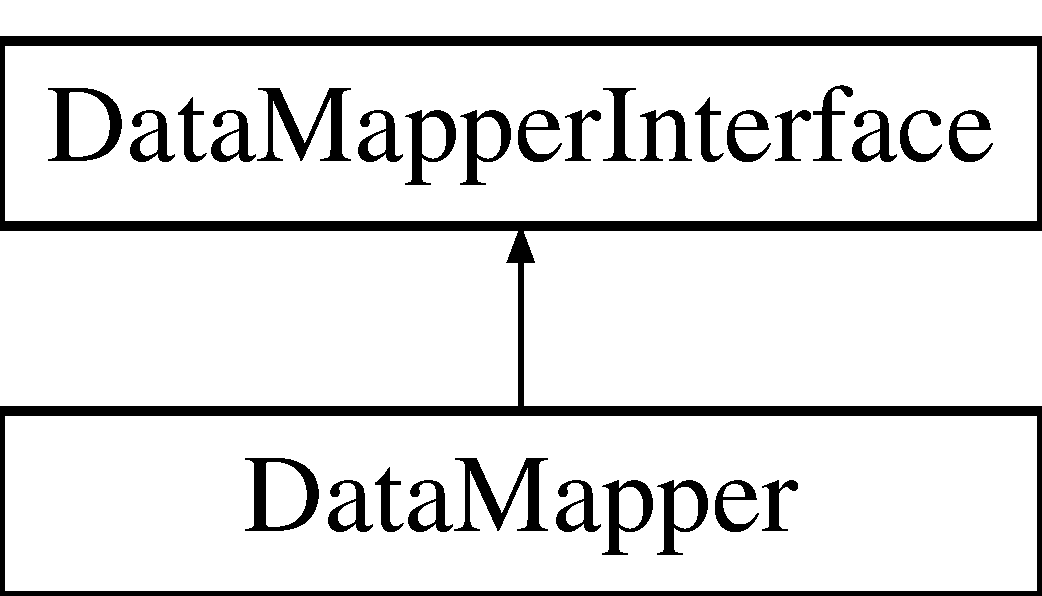
\includegraphics[height=2.000000cm]{d1/d27/class_data_mapper_interface}
\end{center}
\end{figure}
\subsection*{Public Member Functions}
\begin{DoxyCompactItemize}
\item 
virtual void \hyperlink{class_data_mapper_interface_a4a16cab058079e14c1e6169d8038696f}{Update\+Game\+Time\+Database} (std\+::shared\+\_\+ptr$<$ \hyperlink{class_database_interface}{Database\+Interface} $>$ database)=0
\begin{DoxyCompactList}\small\item\em Updates the runtime database with information obtained from an external source or file. \end{DoxyCompactList}\end{DoxyCompactItemize}


\subsection{Detailed Description}
Is the interface used to update the specific \hyperlink{class_database_interface}{Database\+Interface} required for the game. 

\subsection{Member Function Documentation}
\mbox{\Hypertarget{class_data_mapper_interface_a4a16cab058079e14c1e6169d8038696f}\label{class_data_mapper_interface_a4a16cab058079e14c1e6169d8038696f}} 
\index{Data\+Mapper\+Interface@{Data\+Mapper\+Interface}!Update\+Game\+Time\+Database@{Update\+Game\+Time\+Database}}
\index{Update\+Game\+Time\+Database@{Update\+Game\+Time\+Database}!Data\+Mapper\+Interface@{Data\+Mapper\+Interface}}
\subsubsection{\texorpdfstring{Update\+Game\+Time\+Database()}{UpdateGameTimeDatabase()}}
{\footnotesize\ttfamily virtual void Data\+Mapper\+Interface\+::\+Update\+Game\+Time\+Database (\begin{DoxyParamCaption}\item[{std\+::shared\+\_\+ptr$<$ \hyperlink{class_database_interface}{Database\+Interface} $>$}]{database }\end{DoxyParamCaption})\hspace{0.3cm}{\ttfamily [pure virtual]}}



Updates the runtime database with information obtained from an external source or file. 


\begin{DoxyParams}{Parameters}
{\em database} & The database that needs to be updated \\
\hline
\end{DoxyParams}


Implemented in \hyperlink{class_data_mapper_ade3e27146120b3cb74d556e8b9e48526}{Data\+Mapper}.



The documentation for this class was generated from the following file\+:\begin{DoxyCompactItemize}
\item 
C\+:/\+Users/\+Tim/\+Documents/\+Software\+Dev/\+Software\+Project/\+Project\+Files/game-\/source-\/code/\+Back\+End\+Systems/Data\+Mapper\+Interface.\+h\end{DoxyCompactItemize}

\hypertarget{class_delay_component}{}\section{Delay\+Component Class Reference}
\label{class_delay_component}\index{Delay\+Component@{Delay\+Component}}


\hyperlink{class_delay_component}{Delay\+Component} is used to create and manage all delays for the game logic, it uses the delta time value stored within the \hyperlink{class_game_time}{Game\+Time} class.  




{\ttfamily \#include $<$Delay\+Component.\+h$>$}

\subsection*{Public Member Functions}
\begin{DoxyCompactItemize}
\item 
\hyperlink{class_delay_component_a14ff75c76f9e0292f52aadd9e58bec81}{Delay\+Component} (double value, bool Initial\+Use\+Before\+Delay=false)
\begin{DoxyCompactList}\small\item\em Constructor\+: Creates a delay component that uses the specific time value provided. \end{DoxyCompactList}\item 
bool \hyperlink{class_delay_component_a8942e663b1a92471ea79f0e7203d30bc}{Delay\+Finished} ()
\begin{DoxyCompactList}\small\item\em reduces the delay value and then checks if it is finished \end{DoxyCompactList}\item 
\mbox{\Hypertarget{class_delay_component_a539b563338fb30932c96f087dd7a0f5b}\label{class_delay_component_a539b563338fb30932c96f087dd7a0f5b}} 
void \hyperlink{class_delay_component_a539b563338fb30932c96f087dd7a0f5b}{reset\+Delay} ()
\begin{DoxyCompactList}\small\item\em Resets the delay to original value. \end{DoxyCompactList}\end{DoxyCompactItemize}
\subsection*{Private Member Functions}
\begin{DoxyCompactItemize}
\item 
void \hyperlink{class_delay_component_ac2c7023f723523ba2e42ae047d9b6092}{reduce\+Time} ()
\end{DoxyCompactItemize}
\subsection*{Private Attributes}
\begin{DoxyCompactItemize}
\item 
double \hyperlink{class_delay_component_a33d6e279ece1ab6197688c5916dad96d}{\+\_\+current\+Value}
\item 
double \hyperlink{class_delay_component_a36f26c01438d1c0347d06888d3b841ac}{\+\_\+delay\+Value}
\item 
bool \hyperlink{class_delay_component_a821cd453973fced990ae204967e011ff}{\+\_\+delay\+Finished}
\end{DoxyCompactItemize}


\subsection{Detailed Description}
\hyperlink{class_delay_component}{Delay\+Component} is used to create and manage all delays for the game logic, it uses the delta time value stored within the \hyperlink{class_game_time}{Game\+Time} class. 

\subsection{Constructor \& Destructor Documentation}
\mbox{\Hypertarget{class_delay_component_a14ff75c76f9e0292f52aadd9e58bec81}\label{class_delay_component_a14ff75c76f9e0292f52aadd9e58bec81}} 
\index{Delay\+Component@{Delay\+Component}!Delay\+Component@{Delay\+Component}}
\index{Delay\+Component@{Delay\+Component}!Delay\+Component@{Delay\+Component}}
\subsubsection{\texorpdfstring{Delay\+Component()}{DelayComponent()}}
{\footnotesize\ttfamily Delay\+Component\+::\+Delay\+Component (\begin{DoxyParamCaption}\item[{double}]{value,  }\item[{bool}]{Initial\+Use\+Before\+Delay = {\ttfamily false} }\end{DoxyParamCaption})}



Constructor\+: Creates a delay component that uses the specific time value provided. 


\begin{DoxyParams}{Parameters}
{\em value} & The specific time value that represent the length of the delay until it is finished \\
\hline
{\em Initial\+Use\+Before\+Delay} & Allows the client to set whether the delay is initially true until use \\
\hline
\end{DoxyParams}
\begin{DoxyReturn}{Returns}

\end{DoxyReturn}


\subsection{Member Function Documentation}
\mbox{\Hypertarget{class_delay_component_a8942e663b1a92471ea79f0e7203d30bc}\label{class_delay_component_a8942e663b1a92471ea79f0e7203d30bc}} 
\index{Delay\+Component@{Delay\+Component}!Delay\+Finished@{Delay\+Finished}}
\index{Delay\+Finished@{Delay\+Finished}!Delay\+Component@{Delay\+Component}}
\subsubsection{\texorpdfstring{Delay\+Finished()}{DelayFinished()}}
{\footnotesize\ttfamily bool Delay\+Component\+::\+Delay\+Finished (\begin{DoxyParamCaption}{ }\end{DoxyParamCaption})}



reduces the delay value and then checks if it is finished 

\begin{DoxyReturn}{Returns}
Returns true if the delay is finished 
\end{DoxyReturn}
\mbox{\Hypertarget{class_delay_component_ac2c7023f723523ba2e42ae047d9b6092}\label{class_delay_component_ac2c7023f723523ba2e42ae047d9b6092}} 
\index{Delay\+Component@{Delay\+Component}!reduce\+Time@{reduce\+Time}}
\index{reduce\+Time@{reduce\+Time}!Delay\+Component@{Delay\+Component}}
\subsubsection{\texorpdfstring{reduce\+Time()}{reduceTime()}}
{\footnotesize\ttfamily void Delay\+Component\+::reduce\+Time (\begin{DoxyParamCaption}{ }\end{DoxyParamCaption})\hspace{0.3cm}{\ttfamily [private]}}

Reduces the delay time by \hyperlink{class_game_time}{Game\+Time} delta\+Time, is called by Delay\+Finished 

\subsection{Member Data Documentation}
\mbox{\Hypertarget{class_delay_component_a33d6e279ece1ab6197688c5916dad96d}\label{class_delay_component_a33d6e279ece1ab6197688c5916dad96d}} 
\index{Delay\+Component@{Delay\+Component}!\+\_\+current\+Value@{\+\_\+current\+Value}}
\index{\+\_\+current\+Value@{\+\_\+current\+Value}!Delay\+Component@{Delay\+Component}}
\subsubsection{\texorpdfstring{\+\_\+current\+Value}{\_currentValue}}
{\footnotesize\ttfamily double Delay\+Component\+::\+\_\+current\+Value\hspace{0.3cm}{\ttfamily [private]}}

The current value of time until the delay is finished \mbox{\Hypertarget{class_delay_component_a821cd453973fced990ae204967e011ff}\label{class_delay_component_a821cd453973fced990ae204967e011ff}} 
\index{Delay\+Component@{Delay\+Component}!\+\_\+delay\+Finished@{\+\_\+delay\+Finished}}
\index{\+\_\+delay\+Finished@{\+\_\+delay\+Finished}!Delay\+Component@{Delay\+Component}}
\subsubsection{\texorpdfstring{\+\_\+delay\+Finished}{\_delayFinished}}
{\footnotesize\ttfamily bool Delay\+Component\+::\+\_\+delay\+Finished\hspace{0.3cm}{\ttfamily [private]}}

The boolean stored for whether the delay has finished \mbox{\Hypertarget{class_delay_component_a36f26c01438d1c0347d06888d3b841ac}\label{class_delay_component_a36f26c01438d1c0347d06888d3b841ac}} 
\index{Delay\+Component@{Delay\+Component}!\+\_\+delay\+Value@{\+\_\+delay\+Value}}
\index{\+\_\+delay\+Value@{\+\_\+delay\+Value}!Delay\+Component@{Delay\+Component}}
\subsubsection{\texorpdfstring{\+\_\+delay\+Value}{\_delayValue}}
{\footnotesize\ttfamily double Delay\+Component\+::\+\_\+delay\+Value\hspace{0.3cm}{\ttfamily [private]}}

The original value of the delay 

The documentation for this class was generated from the following files\+:\begin{DoxyCompactItemize}
\item 
D\+:/\+Users/\+Tim-\/\+P\+C/\+Documents/\+Software\+\_\+\+I\+I/\+Project/\+Project\+Files/game-\/source-\/code/\+Front\+End\+Systems/Delay\+Component.\+h\item 
D\+:/\+Users/\+Tim-\/\+P\+C/\+Documents/\+Software\+\_\+\+I\+I/\+Project/\+Project\+Files/game-\/source-\/code/\+Front\+End\+Systems/Delay\+Component.\+cpp\end{DoxyCompactItemize}

\hypertarget{class_destroyed_object_outside_scene}{}\section{Destroyed\+Object\+Outside\+Scene Class Reference}
\label{class_destroyed_object_outside_scene}\index{Destroyed\+Object\+Outside\+Scene@{Destroyed\+Object\+Outside\+Scene}}


Exception that is thrown when an object is destroyed and it does not exist inside of a \hyperlink{class_scene}{Scene}.  




{\ttfamily \#include $<$Game\+Object.\+h$>$}



\subsection{Detailed Description}
Exception that is thrown when an object is destroyed and it does not exist inside of a \hyperlink{class_scene}{Scene}. 

The documentation for this class was generated from the following file\+:\begin{DoxyCompactItemize}
\item 
C\+:/\+Users/\+Tim/\+Documents/\+Software\+Dev/\+Software\+Project/\+Project\+Files/game-\/source-\/code/\+Front\+End\+Systems/Game\+Object.\+h\end{DoxyCompactItemize}

\hypertarget{class_display_manager}{}\section{Display\+Manager Class Reference}
\label{class_display_manager}\index{Display\+Manager@{Display\+Manager}}


Display manager is in charge of running and managing the presentation layer.  




{\ttfamily \#include $<$Display\+Manager.\+h$>$}

\subsection*{Public Member Functions}
\begin{DoxyCompactItemize}
\item 
\hyperlink{class_display_manager_a5cae0a0f81cbd2457eca8d35733a0516}{Display\+Manager} (Render\+Window \&render\+Window)
\begin{DoxyCompactList}\small\item\em Constructs the \hyperlink{class_display_manager}{Display\+Manager} Object with the corresponding Render\+Window, initialises the display thread on construction. \end{DoxyCompactList}\item 
\mbox{\Hypertarget{class_display_manager_ab1c3eaf2694410423b6b1eca6a58436f}\label{class_display_manager_ab1c3eaf2694410423b6b1eca6a58436f}} 
void \hyperlink{class_display_manager_ab1c3eaf2694410423b6b1eca6a58436f}{Initialise\+Thread} ()
\begin{DoxyCompactList}\small\item\em used to intialises the display loop for the game inside of a seperate thread \end{DoxyCompactList}\item 
\mbox{\Hypertarget{class_display_manager_ae4c9d79e08490e64602cf562a16d8834}\label{class_display_manager_ae4c9d79e08490e64602cf562a16d8834}} 
\hyperlink{class_display_manager_ae4c9d79e08490e64602cf562a16d8834}{$\sim$\+Display\+Manager} ()
\begin{DoxyCompactList}\small\item\em Destructor sets the \+\_\+displaywindow\+\_\+ptr to null\+\_\+ptr Doesnt delete the window as other objects may still be using it. \end{DoxyCompactList}\end{DoxyCompactItemize}
\subsection*{Private Member Functions}
\begin{DoxyCompactItemize}
\item 
\mbox{\Hypertarget{class_display_manager_a79b7a390f3a2a09e7209d271e589e705}\label{class_display_manager_a79b7a390f3a2a09e7209d271e589e705}} 
void \hyperlink{class_display_manager_a79b7a390f3a2a09e7209d271e589e705}{render\+Thread} ()
\begin{DoxyCompactList}\small\item\em Runs the display loop and is created in a seperate thread. \end{DoxyCompactList}\item 
\mbox{\Hypertarget{class_display_manager_a59cef8980a225ca13757e362a92891d1}\label{class_display_manager_a59cef8980a225ca13757e362a92891d1}} 
void \hyperlink{class_display_manager_a59cef8980a225ca13757e362a92891d1}{Draw} ()
\begin{DoxyCompactList}\small\item\em Draws each sfml sprite object to the game window. \end{DoxyCompactList}\end{DoxyCompactItemize}
\subsection*{Private Attributes}
\begin{DoxyCompactItemize}
\item 
Render\+Window $\ast$ \hyperlink{class_display_manager_abe0369d0fa6b544c77d9d50d50f949cf}{\+\_\+dispwindow\+\_\+ptr}
\item 
\hyperlink{class_update_game_object_display}{Update\+Game\+Object\+Display} \hyperlink{class_display_manager_aee260bf088ffc55e21bd1ef282a139db}{\+\_\+update\+Game\+Object\+Display}
\end{DoxyCompactItemize}


\subsection{Detailed Description}
Display manager is in charge of running and managing the presentation layer. 

It creates a seperate thread which is used to run the display loop. The draw\+Game\+Object class is used to draw each of the \hyperlink{class_game_object}{Game\+Object}\textquotesingle{}s currently being used by the window. 

\subsection{Constructor \& Destructor Documentation}
\mbox{\Hypertarget{class_display_manager_a5cae0a0f81cbd2457eca8d35733a0516}\label{class_display_manager_a5cae0a0f81cbd2457eca8d35733a0516}} 
\index{Display\+Manager@{Display\+Manager}!Display\+Manager@{Display\+Manager}}
\index{Display\+Manager@{Display\+Manager}!Display\+Manager@{Display\+Manager}}
\subsubsection{\texorpdfstring{Display\+Manager()}{DisplayManager()}}
{\footnotesize\ttfamily Display\+Manager\+::\+Display\+Manager (\begin{DoxyParamCaption}\item[{Render\+Window \&}]{render\+Window }\end{DoxyParamCaption})}



Constructs the \hyperlink{class_display_manager}{Display\+Manager} Object with the corresponding Render\+Window, initialises the display thread on construction. 


\begin{DoxyParams}{Parameters}
{\em render\+Window} & \\
\hline
\end{DoxyParams}


\subsection{Member Data Documentation}
\mbox{\Hypertarget{class_display_manager_abe0369d0fa6b544c77d9d50d50f949cf}\label{class_display_manager_abe0369d0fa6b544c77d9d50d50f949cf}} 
\index{Display\+Manager@{Display\+Manager}!\+\_\+dispwindow\+\_\+ptr@{\+\_\+dispwindow\+\_\+ptr}}
\index{\+\_\+dispwindow\+\_\+ptr@{\+\_\+dispwindow\+\_\+ptr}!Display\+Manager@{Display\+Manager}}
\subsubsection{\texorpdfstring{\+\_\+dispwindow\+\_\+ptr}{\_dispwindow\_ptr}}
{\footnotesize\ttfamily Render\+Window$\ast$ Display\+Manager\+::\+\_\+dispwindow\+\_\+ptr\hspace{0.3cm}{\ttfamily [private]}}

A pointer to the corresponding Render\+Window that needs images displayed to it$>$ \mbox{\Hypertarget{class_display_manager_aee260bf088ffc55e21bd1ef282a139db}\label{class_display_manager_aee260bf088ffc55e21bd1ef282a139db}} 
\index{Display\+Manager@{Display\+Manager}!\+\_\+update\+Game\+Object\+Display@{\+\_\+update\+Game\+Object\+Display}}
\index{\+\_\+update\+Game\+Object\+Display@{\+\_\+update\+Game\+Object\+Display}!Display\+Manager@{Display\+Manager}}
\subsubsection{\texorpdfstring{\+\_\+update\+Game\+Object\+Display}{\_updateGameObjectDisplay}}
{\footnotesize\ttfamily \hyperlink{class_update_game_object_display}{Update\+Game\+Object\+Display} Display\+Manager\+::\+\_\+update\+Game\+Object\+Display\hspace{0.3cm}{\ttfamily [private]}}

Composition object responsible for displaying each \hyperlink{class_game_object}{Game\+Object} and the its corresponding Sprite$>$ 

The documentation for this class was generated from the following files\+:\begin{DoxyCompactItemize}
\item 
C\+:/\+Users/\+Tim/\+Documents/\+Software\+Dev/\+Software\+Project/\+Project\+Files/game-\/source-\/code/\+Back\+End\+Systems/Display\+Manager.\+h\item 
C\+:/\+Users/\+Tim/\+Documents/\+Software\+Dev/\+Software\+Project/\+Project\+Files/game-\/source-\/code/\+Back\+End\+Systems/Display\+Manger.\+cpp\end{DoxyCompactItemize}

\hypertarget{class_enemy}{}\section{Enemy Class Reference}
\label{class_enemy}\index{Enemy@{Enemy}}


The basic \hyperlink{class_enemy}{Enemy} Object representation.  




{\ttfamily \#include $<$Enemy.\+h$>$}

Inheritance diagram for Enemy\+:\begin{figure}[H]
\begin{center}
\leavevmode
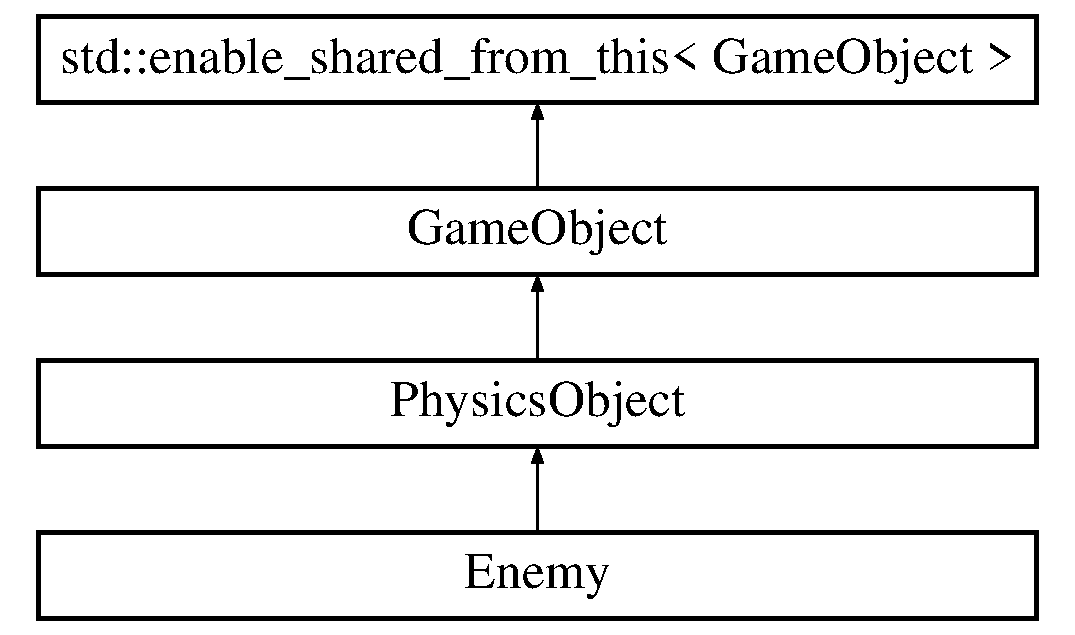
\includegraphics[height=4.000000cm]{dd/d7a/class_enemy}
\end{center}
\end{figure}
\subsection*{Public Member Functions}
\begin{DoxyCompactItemize}
\item 
\hyperlink{class_enemy_a0e382a7495bdbb9b802d1ed3931b4fc1}{Enemy} (const \hyperlink{class_physics_object}{Physics\+Object} \&physics\+Object, const double \&shoot\+Delay, const std\+::shared\+\_\+ptr$<$ \hyperlink{class_movable_interface}{Movable\+Interface} $>$ \&move\+Comp, const std\+::shared\+\_\+ptr$<$ \hyperlink{class_shoot_interface}{Shoot\+Interface} $>$ \&shoot\+Comp)
\begin{DoxyCompactList}\small\item\em Constructs the main enemy object used within the game. \end{DoxyCompactList}\item 
virtual void \hyperlink{class_enemy_a64ee0cc6fb8a3424d486537efb8205d8}{Start} () override
\begin{DoxyCompactList}\small\item\em Used to initialise the \hyperlink{class_enemy}{Enemy}. \end{DoxyCompactList}\item 
\mbox{\Hypertarget{class_enemy_a614ad271f07ecf63cb3e665155b7e258}\label{class_enemy_a614ad271f07ecf63cb3e665155b7e258}} 
virtual void \hyperlink{class_enemy_a614ad271f07ecf63cb3e665155b7e258}{Update} () override
\begin{DoxyCompactList}\small\item\em Runs once a frame and updates the various methods and members of the enemy. \end{DoxyCompactList}\item 
virtual void \hyperlink{class_enemy_ac59660a58fac8d0ffdcb97c0717fa089}{collision\+Action} (const Game\+Object\+Type \&object\+Type) override
\begin{DoxyCompactList}\small\item\em Checks if the enemy has collided with a player or player projectile and responds accordingly. \end{DoxyCompactList}\item 
void \hyperlink{class_enemy_a7fc3561fe6b79712b51bd06fa8ce24d0}{Assign\+Enemy\+Controller} (const std\+::shared\+\_\+ptr$<$ \hyperlink{class_game_object}{Game\+Object} $>$ \&enemy\+Controller)
\begin{DoxyCompactList}\small\item\em Assigns an enemy controller to the specific enemy, used to communicate with the enemy controller so that it knows whenever an enemy is destroyed. \end{DoxyCompactList}\item 
\mbox{\Hypertarget{class_enemy_aafb628c66008e33afdd750e2f492bd98}\label{class_enemy_aafb628c66008e33afdd750e2f492bd98}} 
virtual \hyperlink{class_enemy_aafb628c66008e33afdd750e2f492bd98}{$\sim$\+Enemy} ()=default
\begin{DoxyCompactList}\small\item\em Default Destructor. \end{DoxyCompactList}\end{DoxyCompactItemize}
\subsection*{Private Member Functions}
\begin{DoxyCompactItemize}
\item 
\mbox{\Hypertarget{class_enemy_ab526cfaf13910e15ca1e5e84ef230dd1}\label{class_enemy_ab526cfaf13910e15ca1e5e84ef230dd1}} 
void \hyperlink{class_enemy_ab526cfaf13910e15ca1e5e84ef230dd1}{Shoot} ()
\begin{DoxyCompactList}\small\item\em Determines if the shoot\+Delay is finished, if it is an \hyperlink{class_enemy_projectile}{Enemy\+Projectile} is created using the shoot\+Comp. \end{DoxyCompactList}\item 
\mbox{\Hypertarget{class_enemy_a06fafdc67bd76334adb9d47f73f15aff}\label{class_enemy_a06fafdc67bd76334adb9d47f73f15aff}} 
void \hyperlink{class_enemy_a06fafdc67bd76334adb9d47f73f15aff}{Check\+Outside\+Screen} ()
\begin{DoxyCompactList}\small\item\em Checks if the enemy is out of screen bounds. \end{DoxyCompactList}\item 
\hyperlink{class_vector2_d}{Vector2D} \hyperlink{class_enemy_aa40cb40a3a2d83e82e02ee5cfbb9ee96}{Generate\+Random\+Move\+Direction} ()
\begin{DoxyCompactList}\small\item\em Generates the random direction for the object to move in. \end{DoxyCompactList}\item 
\mbox{\Hypertarget{class_enemy_a9c4e7e1c9f79650d1f0dd3c72ae9c82d}\label{class_enemy_a9c4e7e1c9f79650d1f0dd3c72ae9c82d}} 
void \hyperlink{class_enemy_a9c4e7e1c9f79650d1f0dd3c72ae9c82d}{Player\+Projectile\+Collision} ()
\begin{DoxyCompactList}\small\item\em The Response of an Enemy\+Obejct to colliding with the player or the player bullet. \end{DoxyCompactList}\end{DoxyCompactItemize}
\subsection*{Private Attributes}
\begin{DoxyCompactItemize}
\item 
\hyperlink{class_delay_component}{Delay\+Component} \hyperlink{class_enemy_a3c5bc99471cfa718af8e11b3b735d15c}{\+\_\+shoot\+Delay}
\item 
std\+::shared\+\_\+ptr$<$ \hyperlink{class_shoot_interface}{Shoot\+Interface} $>$ \hyperlink{class_enemy_aab1e06a64c7fc2d07d40522a7a7cf8be}{\+\_\+enemy\+Shoot}
\item 
\hyperlink{class_boundary}{Boundary} \hyperlink{class_enemy_afb32f85ca2f3dce003e62a91572bdb70}{\+\_\+screen\+Bounds}
\item 
\hyperlink{class_size_reduction}{Size\+Reduction} \hyperlink{class_enemy_af8b4d39339f59407b7fd9cd1d6246860}{\+\_\+size\+Reduction}
\item 
std\+::shared\+\_\+ptr$<$ \hyperlink{class_movable_interface}{Movable\+Interface} $>$ \hyperlink{class_enemy_a1776f87f0a6993e9e3255c8a41c73809}{\+\_\+move\+Comp}
\item 
std\+::shared\+\_\+ptr$<$ \hyperlink{class_enemy_controller}{Enemy\+Controller} $>$ \hyperlink{class_enemy_acc360bdd3b46cea29891f534af2153c8}{\+\_\+enemy\+Controller}
\end{DoxyCompactItemize}
\subsection*{Additional Inherited Members}


\subsection{Detailed Description}
The basic \hyperlink{class_enemy}{Enemy} Object representation. 

Uses various interface composition objects to vary the behaviour of the \hyperlink{class_enemy}{Enemy} Object 

\subsection{Constructor \& Destructor Documentation}
\mbox{\Hypertarget{class_enemy_a0e382a7495bdbb9b802d1ed3931b4fc1}\label{class_enemy_a0e382a7495bdbb9b802d1ed3931b4fc1}} 
\index{Enemy@{Enemy}!Enemy@{Enemy}}
\index{Enemy@{Enemy}!Enemy@{Enemy}}
\subsubsection{\texorpdfstring{Enemy()}{Enemy()}}
{\footnotesize\ttfamily Enemy\+::\+Enemy (\begin{DoxyParamCaption}\item[{const \hyperlink{class_physics_object}{Physics\+Object} \&}]{physics\+Object,  }\item[{const double \&}]{shoot\+Delay,  }\item[{const std\+::shared\+\_\+ptr$<$ \hyperlink{class_movable_interface}{Movable\+Interface} $>$ \&}]{move\+Comp,  }\item[{const std\+::shared\+\_\+ptr$<$ \hyperlink{class_shoot_interface}{Shoot\+Interface} $>$ \&}]{shoot\+Comp }\end{DoxyParamCaption})}



Constructs the main enemy object used within the game. 


\begin{DoxyParams}{Parameters}
{\em physics\+Object} & The physics object information used to construct the enemy \\
\hline
{\em shoot\+Delay} & The \hyperlink{class_delay_component}{Delay\+Component} specified between enemy shots \\
\hline
{\em move\+Comp} & the \hyperlink{class_movable_interface}{Movable\+Interface} that the enemy uses \\
\hline
{\em shoot\+Comp} & The \hyperlink{class_shoot_interface}{Shoot\+Interface} used by the enemy\\
\hline
{\em physics\+Object} & \\
\hline
{\em shoot\+Delay} & \\
\hline
{\em move\+Comp} & \\
\hline
{\em shoot\+Comp} & \\
\hline
\end{DoxyParams}


\subsection{Member Function Documentation}
\mbox{\Hypertarget{class_enemy_a7fc3561fe6b79712b51bd06fa8ce24d0}\label{class_enemy_a7fc3561fe6b79712b51bd06fa8ce24d0}} 
\index{Enemy@{Enemy}!Assign\+Enemy\+Controller@{Assign\+Enemy\+Controller}}
\index{Assign\+Enemy\+Controller@{Assign\+Enemy\+Controller}!Enemy@{Enemy}}
\subsubsection{\texorpdfstring{Assign\+Enemy\+Controller()}{AssignEnemyController()}}
{\footnotesize\ttfamily void Enemy\+::\+Assign\+Enemy\+Controller (\begin{DoxyParamCaption}\item[{const std\+::shared\+\_\+ptr$<$ \hyperlink{class_game_object}{Game\+Object} $>$ \&}]{enemy\+Controller }\end{DoxyParamCaption})}



Assigns an enemy controller to the specific enemy, used to communicate with the enemy controller so that it knows whenever an enemy is destroyed. 


\begin{DoxyParams}{Parameters}
{\em enemy\+Controller} & shared pointer to the \hyperlink{class_enemy_controller}{Enemy\+Controller} that created the enemy \\
\hline
\end{DoxyParams}
\mbox{\Hypertarget{class_enemy_ac59660a58fac8d0ffdcb97c0717fa089}\label{class_enemy_ac59660a58fac8d0ffdcb97c0717fa089}} 
\index{Enemy@{Enemy}!collision\+Action@{collision\+Action}}
\index{collision\+Action@{collision\+Action}!Enemy@{Enemy}}
\subsubsection{\texorpdfstring{collision\+Action()}{collisionAction()}}
{\footnotesize\ttfamily void Enemy\+::collision\+Action (\begin{DoxyParamCaption}\item[{const Game\+Object\+Type \&}]{object\+Type }\end{DoxyParamCaption})\hspace{0.3cm}{\ttfamily [override]}, {\ttfamily [virtual]}}



Checks if the enemy has collided with a player or player projectile and responds accordingly. 


\begin{DoxyParams}{Parameters}
{\em object\+Type} & The type of object that has collided with the enemy \\
\hline
\end{DoxyParams}


Reimplemented from \hyperlink{class_physics_object_a16163f4e5bf781b3814d024c9f44a276}{Physics\+Object}.

\mbox{\Hypertarget{class_enemy_aa40cb40a3a2d83e82e02ee5cfbb9ee96}\label{class_enemy_aa40cb40a3a2d83e82e02ee5cfbb9ee96}} 
\index{Enemy@{Enemy}!Generate\+Random\+Move\+Direction@{Generate\+Random\+Move\+Direction}}
\index{Generate\+Random\+Move\+Direction@{Generate\+Random\+Move\+Direction}!Enemy@{Enemy}}
\subsubsection{\texorpdfstring{Generate\+Random\+Move\+Direction()}{GenerateRandomMoveDirection()}}
{\footnotesize\ttfamily \hyperlink{class_vector2_d}{Vector2D} Enemy\+::\+Generate\+Random\+Move\+Direction (\begin{DoxyParamCaption}{ }\end{DoxyParamCaption})\hspace{0.3cm}{\ttfamily [private]}}



Generates the random direction for the object to move in. 

\begin{DoxyReturn}{Returns}
Returns the generated random direction 
\end{DoxyReturn}
\mbox{\Hypertarget{class_enemy_a64ee0cc6fb8a3424d486537efb8205d8}\label{class_enemy_a64ee0cc6fb8a3424d486537efb8205d8}} 
\index{Enemy@{Enemy}!Start@{Start}}
\index{Start@{Start}!Enemy@{Enemy}}
\subsubsection{\texorpdfstring{Start()}{Start()}}
{\footnotesize\ttfamily void Enemy\+::\+Start (\begin{DoxyParamCaption}{ }\end{DoxyParamCaption})\hspace{0.3cm}{\ttfamily [override]}, {\ttfamily [virtual]}}



Used to initialise the \hyperlink{class_enemy}{Enemy}. 

ensures that the enemy is scaled correctly before it is displayed, and generates a random direction for its movement 

Reimplemented from \hyperlink{class_game_object_aeeb2162f2779e5591a372a1568bc5c68}{Game\+Object}.



\subsection{Member Data Documentation}
\mbox{\Hypertarget{class_enemy_acc360bdd3b46cea29891f534af2153c8}\label{class_enemy_acc360bdd3b46cea29891f534af2153c8}} 
\index{Enemy@{Enemy}!\+\_\+enemy\+Controller@{\+\_\+enemy\+Controller}}
\index{\+\_\+enemy\+Controller@{\+\_\+enemy\+Controller}!Enemy@{Enemy}}
\subsubsection{\texorpdfstring{\+\_\+enemy\+Controller}{\_enemyController}}
{\footnotesize\ttfamily std\+::shared\+\_\+ptr$<$\hyperlink{class_enemy_controller}{Enemy\+Controller}$>$ Enemy\+::\+\_\+enemy\+Controller\hspace{0.3cm}{\ttfamily [private]}}

\hyperlink{class_enemy_controller}{Enemy\+Controller} used to create the enemy object, is notified when the \hyperlink{class_enemy}{Enemy} object is destroyed \mbox{\Hypertarget{class_enemy_aab1e06a64c7fc2d07d40522a7a7cf8be}\label{class_enemy_aab1e06a64c7fc2d07d40522a7a7cf8be}} 
\index{Enemy@{Enemy}!\+\_\+enemy\+Shoot@{\+\_\+enemy\+Shoot}}
\index{\+\_\+enemy\+Shoot@{\+\_\+enemy\+Shoot}!Enemy@{Enemy}}
\subsubsection{\texorpdfstring{\+\_\+enemy\+Shoot}{\_enemyShoot}}
{\footnotesize\ttfamily std\+::shared\+\_\+ptr$<$\hyperlink{class_shoot_interface}{Shoot\+Interface}$>$ Enemy\+::\+\_\+enemy\+Shoot\hspace{0.3cm}{\ttfamily [private]}}

\hyperlink{class_shoot_interface}{Shoot\+Interface} used to specify the specific type of shooting \mbox{\Hypertarget{class_enemy_a1776f87f0a6993e9e3255c8a41c73809}\label{class_enemy_a1776f87f0a6993e9e3255c8a41c73809}} 
\index{Enemy@{Enemy}!\+\_\+move\+Comp@{\+\_\+move\+Comp}}
\index{\+\_\+move\+Comp@{\+\_\+move\+Comp}!Enemy@{Enemy}}
\subsubsection{\texorpdfstring{\+\_\+move\+Comp}{\_moveComp}}
{\footnotesize\ttfamily std\+::shared\+\_\+ptr$<$\hyperlink{class_movable_interface}{Movable\+Interface}$>$ Enemy\+::\+\_\+move\+Comp\hspace{0.3cm}{\ttfamily [private]}}

Moveable\+Interface used to move the enemy in a specific way \mbox{\Hypertarget{class_enemy_afb32f85ca2f3dce003e62a91572bdb70}\label{class_enemy_afb32f85ca2f3dce003e62a91572bdb70}} 
\index{Enemy@{Enemy}!\+\_\+screen\+Bounds@{\+\_\+screen\+Bounds}}
\index{\+\_\+screen\+Bounds@{\+\_\+screen\+Bounds}!Enemy@{Enemy}}
\subsubsection{\texorpdfstring{\+\_\+screen\+Bounds}{\_screenBounds}}
{\footnotesize\ttfamily \hyperlink{class_boundary}{Boundary} Enemy\+::\+\_\+screen\+Bounds\hspace{0.3cm}{\ttfamily [private]}}

Default boundary used to test if the enemy is outside of the screen \mbox{\Hypertarget{class_enemy_a3c5bc99471cfa718af8e11b3b735d15c}\label{class_enemy_a3c5bc99471cfa718af8e11b3b735d15c}} 
\index{Enemy@{Enemy}!\+\_\+shoot\+Delay@{\+\_\+shoot\+Delay}}
\index{\+\_\+shoot\+Delay@{\+\_\+shoot\+Delay}!Enemy@{Enemy}}
\subsubsection{\texorpdfstring{\+\_\+shoot\+Delay}{\_shootDelay}}
{\footnotesize\ttfamily \hyperlink{class_delay_component}{Delay\+Component} Enemy\+::\+\_\+shoot\+Delay\hspace{0.3cm}{\ttfamily [private]}}

delay used between each shot per object \mbox{\Hypertarget{class_enemy_af8b4d39339f59407b7fd9cd1d6246860}\label{class_enemy_af8b4d39339f59407b7fd9cd1d6246860}} 
\index{Enemy@{Enemy}!\+\_\+size\+Reduction@{\+\_\+size\+Reduction}}
\index{\+\_\+size\+Reduction@{\+\_\+size\+Reduction}!Enemy@{Enemy}}
\subsubsection{\texorpdfstring{\+\_\+size\+Reduction}{\_sizeReduction}}
{\footnotesize\ttfamily \hyperlink{class_size_reduction}{Size\+Reduction} Enemy\+::\+\_\+size\+Reduction\hspace{0.3cm}{\ttfamily [private]}}

\hyperlink{class_size_reduction}{Size\+Reduction} component used to scale the enemy as it moves towards or away from the centre of the screen 

The documentation for this class was generated from the following files\+:\begin{DoxyCompactItemize}
\item 
D\+:/\+Users/\+Tim-\/\+P\+C/\+Documents/\+Software\+\_\+\+I\+I/\+Project/\+Project\+Files/game-\/source-\/code/\+Front\+End\+Systems/Enemy.\+h\item 
D\+:/\+Users/\+Tim-\/\+P\+C/\+Documents/\+Software\+\_\+\+I\+I/\+Project/\+Project\+Files/game-\/source-\/code/\+Front\+End\+Systems/Enemy.\+cpp\end{DoxyCompactItemize}

\hypertarget{class_enemy_controller}{}\section{Enemy\+Controller Class Reference}
\label{class_enemy_controller}\index{Enemy\+Controller@{Enemy\+Controller}}


\hyperlink{class_enemy}{Enemy} controller is responsible for spawning and monitoring new enemy objects.  




{\ttfamily \#include $<$Enemy\+Controller.\+h$>$}

Inheritance diagram for Enemy\+Controller\+:\begin{figure}[H]
\begin{center}
\leavevmode
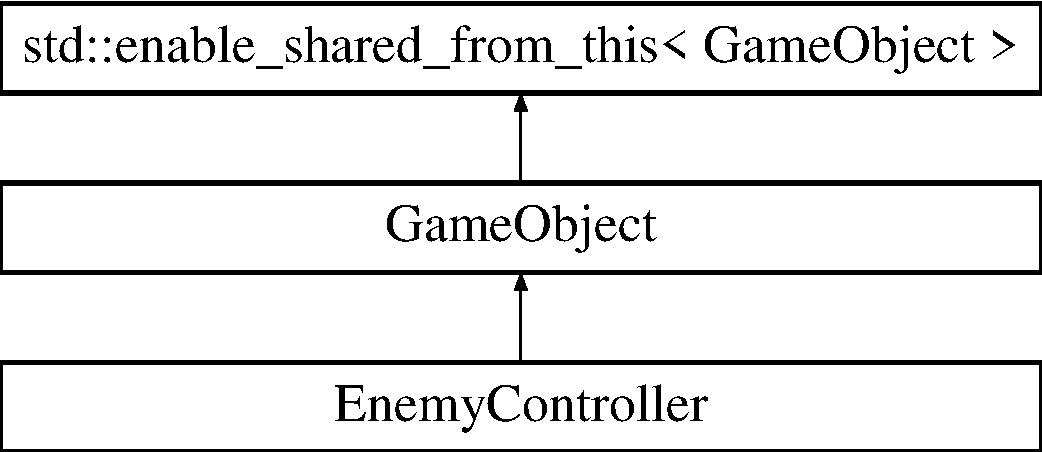
\includegraphics[height=3.000000cm]{dc/d01/class_enemy_controller}
\end{center}
\end{figure}
\subsection*{Public Member Functions}
\begin{DoxyCompactItemize}
\item 
\hyperlink{class_enemy_controller_a07159de6348f511017c5415371459d50}{Enemy\+Controller} (const \hyperlink{class_game_object}{Game\+Object} \&game\+Object, unsigned int max\+\_\+enemies, double enemy\+Spawn\+Delay)
\begin{DoxyCompactList}\small\item\em Constructs an \hyperlink{class_enemy_controller}{Enemy\+Controller} Object. \end{DoxyCompactList}\item 
\mbox{\Hypertarget{class_enemy_controller_af36ec67442d30c7519581b83ad6c00db}\label{class_enemy_controller_af36ec67442d30c7519581b83ad6c00db}} 
virtual void \hyperlink{class_enemy_controller_af36ec67442d30c7519581b83ad6c00db}{Update} () override
\begin{DoxyCompactList}\small\item\em Creates enemies based on the spawn delay. \end{DoxyCompactList}\item 
\mbox{\Hypertarget{class_enemy_controller_a011030dd51b78317ecb16356bf6591dc}\label{class_enemy_controller_a011030dd51b78317ecb16356bf6591dc}} 
void \hyperlink{class_enemy_controller_a011030dd51b78317ecb16356bf6591dc}{Enemy\+Killed} ()
\begin{DoxyCompactList}\small\item\em Called by the Enemy\+Object to inform the \hyperlink{class_enemy_controller}{Enemy\+Controller} that it has been destroyed by the \hyperlink{class_player}{Player} object. \end{DoxyCompactList}\item 
void \hyperlink{class_enemy_controller_a182dba707716f8079bb6e67e8c5ed4ad}{Enemy\+Outof\+Bounds} ()
\begin{DoxyCompactList}\small\item\em Called by the Enemy\+Object to inform the \hyperlink{class_enemy_controller}{Enemy\+Controller} that it has been destroyed by the moving out of bounds. \end{DoxyCompactList}\end{DoxyCompactItemize}
\subsection*{Private Member Functions}
\begin{DoxyCompactItemize}
\item 
\mbox{\Hypertarget{class_enemy_controller_a84eabc12a38617b5ff05c6e896e97531}\label{class_enemy_controller_a84eabc12a38617b5ff05c6e896e97531}} 
void \hyperlink{class_enemy_controller_a84eabc12a38617b5ff05c6e896e97531}{Spawn\+Enemy\+Count\+Down} ()
\begin{DoxyCompactList}\small\item\em Checks if an \hyperlink{class_enemy}{Enemy} can be spawned due to the spawn delay, calls Spawn\+Enemy if it can be. \end{DoxyCompactList}\item 
\mbox{\Hypertarget{class_enemy_controller_ab5298e79a0bf598ed8684efb8a6a3927}\label{class_enemy_controller_ab5298e79a0bf598ed8684efb8a6a3927}} 
void \hyperlink{class_enemy_controller_ab5298e79a0bf598ed8684efb8a6a3927}{Spawn\+Enemy} ()
\begin{DoxyCompactList}\small\item\em Creates an enemy and adds it to the same \hyperlink{class_scene}{Scene} as the \hyperlink{class_enemy_controller}{Enemy\+Controller}. \end{DoxyCompactList}\end{DoxyCompactItemize}
\subsection*{Private Attributes}
\begin{DoxyCompactItemize}
\item 
unsigned int \hyperlink{class_enemy_controller_a2b2fdb5b40b75f719838da0386861da5}{number\+Of\+Enemies\+Killed}
\item 
const unsigned int \hyperlink{class_enemy_controller_aca04264b909526dadc67a41f8c826aee}{M\+A\+X\+\_\+\+N\+U\+M\+B\+E\+R\+\_\+\+O\+F\+\_\+\+E\+N\+E\+M\+I\+ES}
\item 
\hyperlink{class_delay_component}{Delay\+Component} \hyperlink{class_enemy_controller_af6136b2e8750227e8adf729c9de5232b}{\+\_\+enemy\+Spawn\+Delay}
\item 
unsigned int \hyperlink{class_enemy_controller_a673e9320e737999189b943216f6d379b}{enemy\+Count}
\end{DoxyCompactItemize}
\subsection*{Additional Inherited Members}


\subsection{Detailed Description}
\hyperlink{class_enemy}{Enemy} controller is responsible for spawning and monitoring new enemy objects. 

The number of enemies spawned and destroyed is moitored. When an enemy goes out of bounds it is destroyed and created a new. The enemy objects have access to the \hyperlink{class_enemy_controller}{Enemy\+Controller} to communicate with it when they are destroyed by the player and when they leave the bounds of the screen. If all the enemies have been destroyed the \hyperlink{class_enemy_controller}{Enemy\+Controller} changes scenes to the Win\+Screen 

\subsection{Constructor \& Destructor Documentation}
\mbox{\Hypertarget{class_enemy_controller_a07159de6348f511017c5415371459d50}\label{class_enemy_controller_a07159de6348f511017c5415371459d50}} 
\index{Enemy\+Controller@{Enemy\+Controller}!Enemy\+Controller@{Enemy\+Controller}}
\index{Enemy\+Controller@{Enemy\+Controller}!Enemy\+Controller@{Enemy\+Controller}}
\subsubsection{\texorpdfstring{Enemy\+Controller()}{EnemyController()}}
{\footnotesize\ttfamily Enemy\+Controller\+::\+Enemy\+Controller (\begin{DoxyParamCaption}\item[{const \hyperlink{class_game_object}{Game\+Object} \&}]{game\+Object,  }\item[{unsigned int}]{max\+\_\+enemies,  }\item[{double}]{enemy\+Spawn\+Delay }\end{DoxyParamCaption})}



Constructs an \hyperlink{class_enemy_controller}{Enemy\+Controller} Object. 


\begin{DoxyParams}{Parameters}
{\em max\+\_\+enemies} & The maximum number of enemies that the \hyperlink{class_enemy_controller}{Enemy\+Controller} will create \\
\hline
{\em enemy\+Spawn\+Delay} & The time delay between spawning an enemy object \\
\hline
\end{DoxyParams}


\subsection{Member Function Documentation}
\mbox{\Hypertarget{class_enemy_controller_a182dba707716f8079bb6e67e8c5ed4ad}\label{class_enemy_controller_a182dba707716f8079bb6e67e8c5ed4ad}} 
\index{Enemy\+Controller@{Enemy\+Controller}!Enemy\+Outof\+Bounds@{Enemy\+Outof\+Bounds}}
\index{Enemy\+Outof\+Bounds@{Enemy\+Outof\+Bounds}!Enemy\+Controller@{Enemy\+Controller}}
\subsubsection{\texorpdfstring{Enemy\+Outof\+Bounds()}{EnemyOutofBounds()}}
{\footnotesize\ttfamily void Enemy\+Controller\+::\+Enemy\+Outof\+Bounds (\begin{DoxyParamCaption}{ }\end{DoxyParamCaption})}



Called by the Enemy\+Object to inform the \hyperlink{class_enemy_controller}{Enemy\+Controller} that it has been destroyed by the moving out of bounds. 

spawns a new enemy without checking the delay as the enemy has already been spawned 

\subsection{Member Data Documentation}
\mbox{\Hypertarget{class_enemy_controller_af6136b2e8750227e8adf729c9de5232b}\label{class_enemy_controller_af6136b2e8750227e8adf729c9de5232b}} 
\index{Enemy\+Controller@{Enemy\+Controller}!\+\_\+enemy\+Spawn\+Delay@{\+\_\+enemy\+Spawn\+Delay}}
\index{\+\_\+enemy\+Spawn\+Delay@{\+\_\+enemy\+Spawn\+Delay}!Enemy\+Controller@{Enemy\+Controller}}
\subsubsection{\texorpdfstring{\+\_\+enemy\+Spawn\+Delay}{\_enemySpawnDelay}}
{\footnotesize\ttfamily \hyperlink{class_delay_component}{Delay\+Component} Enemy\+Controller\+::\+\_\+enemy\+Spawn\+Delay\hspace{0.3cm}{\ttfamily [private]}}

The delay component used to track the delay between enemy spawns \mbox{\Hypertarget{class_enemy_controller_a673e9320e737999189b943216f6d379b}\label{class_enemy_controller_a673e9320e737999189b943216f6d379b}} 
\index{Enemy\+Controller@{Enemy\+Controller}!enemy\+Count@{enemy\+Count}}
\index{enemy\+Count@{enemy\+Count}!Enemy\+Controller@{Enemy\+Controller}}
\subsubsection{\texorpdfstring{enemy\+Count}{enemyCount}}
{\footnotesize\ttfamily unsigned int Enemy\+Controller\+::enemy\+Count\hspace{0.3cm}{\ttfamily [private]}}

The current number of enemies that have been spawned \mbox{\Hypertarget{class_enemy_controller_aca04264b909526dadc67a41f8c826aee}\label{class_enemy_controller_aca04264b909526dadc67a41f8c826aee}} 
\index{Enemy\+Controller@{Enemy\+Controller}!M\+A\+X\+\_\+\+N\+U\+M\+B\+E\+R\+\_\+\+O\+F\+\_\+\+E\+N\+E\+M\+I\+ES@{M\+A\+X\+\_\+\+N\+U\+M\+B\+E\+R\+\_\+\+O\+F\+\_\+\+E\+N\+E\+M\+I\+ES}}
\index{M\+A\+X\+\_\+\+N\+U\+M\+B\+E\+R\+\_\+\+O\+F\+\_\+\+E\+N\+E\+M\+I\+ES@{M\+A\+X\+\_\+\+N\+U\+M\+B\+E\+R\+\_\+\+O\+F\+\_\+\+E\+N\+E\+M\+I\+ES}!Enemy\+Controller@{Enemy\+Controller}}
\subsubsection{\texorpdfstring{M\+A\+X\+\_\+\+N\+U\+M\+B\+E\+R\+\_\+\+O\+F\+\_\+\+E\+N\+E\+M\+I\+ES}{MAX\_NUMBER\_OF\_ENEMIES}}
{\footnotesize\ttfamily const unsigned int Enemy\+Controller\+::\+M\+A\+X\+\_\+\+N\+U\+M\+B\+E\+R\+\_\+\+O\+F\+\_\+\+E\+N\+E\+M\+I\+ES\hspace{0.3cm}{\ttfamily [private]}}

The maximum number of enemies that the \hyperlink{class_enemy_controller}{Enemy\+Controller} can create \mbox{\Hypertarget{class_enemy_controller_a2b2fdb5b40b75f719838da0386861da5}\label{class_enemy_controller_a2b2fdb5b40b75f719838da0386861da5}} 
\index{Enemy\+Controller@{Enemy\+Controller}!number\+Of\+Enemies\+Killed@{number\+Of\+Enemies\+Killed}}
\index{number\+Of\+Enemies\+Killed@{number\+Of\+Enemies\+Killed}!Enemy\+Controller@{Enemy\+Controller}}
\subsubsection{\texorpdfstring{number\+Of\+Enemies\+Killed}{numberOfEnemiesKilled}}
{\footnotesize\ttfamily unsigned int Enemy\+Controller\+::number\+Of\+Enemies\+Killed\hspace{0.3cm}{\ttfamily [private]}}

Tracks the number of enemies that the player has destroyed 

The documentation for this class was generated from the following files\+:\begin{DoxyCompactItemize}
\item 
C\+:/\+Users/\+Tim/\+Documents/\+Software\+Dev/\+Software\+Project/\+Project\+Files/game-\/source-\/code/\+Front\+End\+Systems/Enemy\+Controller.\+h\item 
C\+:/\+Users/\+Tim/\+Documents/\+Software\+Dev/\+Software\+Project/\+Project\+Files/game-\/source-\/code/\+Front\+End\+Systems/Enemy\+Controller.\+cpp\end{DoxyCompactItemize}

\hypertarget{class_enemy_controller_factory}{}\section{Enemy\+Controller\+Factory Class Reference}
\label{class_enemy_controller_factory}\index{Enemy\+Controller\+Factory@{Enemy\+Controller\+Factory}}


\hyperlink{class_enemy_controller_factory}{Enemy\+Controller\+Factory} is responsible for the construction of any \hyperlink{class_enemy_controller}{Enemy\+Controller} objects.  




{\ttfamily \#include $<$Enemy\+Controller\+Factory.\+h$>$}

Inheritance diagram for Enemy\+Controller\+Factory\+:\begin{figure}[H]
\begin{center}
\leavevmode
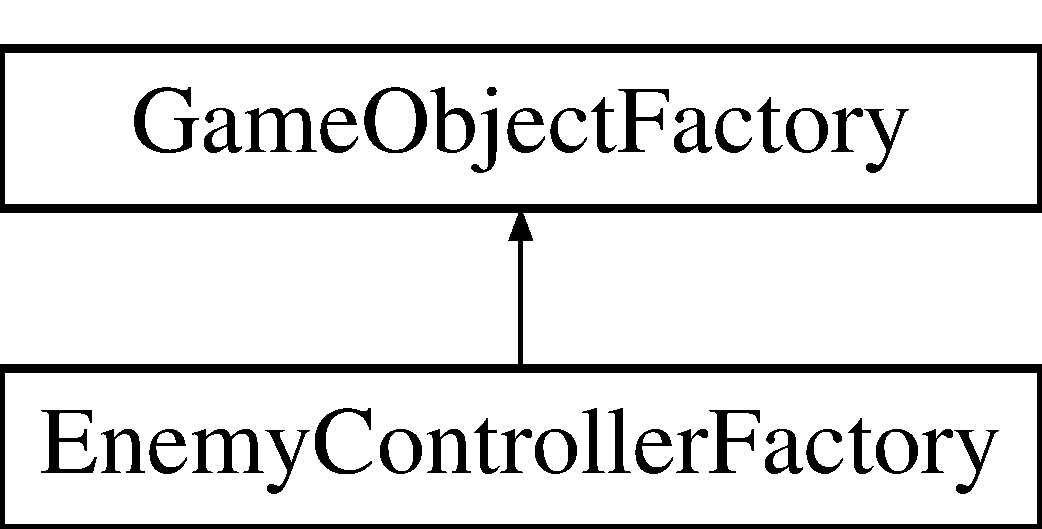
\includegraphics[height=2.000000cm]{d5/d7d/class_enemy_controller_factory}
\end{center}
\end{figure}
\subsection*{Public Member Functions}
\begin{DoxyCompactItemize}
\item 
virtual std\+::shared\+\_\+ptr$<$ \hyperlink{class_game_object}{Game\+Object} $>$ \hyperlink{class_enemy_controller_factory_a6ab6c433cc498c7353a1ab2eb213664d}{get\+Game\+Object} (const std\+::shared\+\_\+ptr$<$ \hyperlink{class_database_interface}{Database\+Interface} $>$ \&database) override
\begin{DoxyCompactList}\small\item\em Function call used to create an \hyperlink{class_enemy_controller}{Enemy\+Controller} Object. \end{DoxyCompactList}\item 
virtual \hyperlink{struct_game_object_data}{Game\+Object\+Data} \hyperlink{class_enemy_controller_factory_a27d4819c1174490c22f2e111f32ca2ec}{get\+Object\+Data} (const std\+::shared\+\_\+ptr$<$ \hyperlink{class_database_interface}{Database\+Interface} $>$ \&database) override
\begin{DoxyCompactList}\small\item\em used to obtain the specific \hyperlink{struct_game_object_data}{Game\+Object\+Data} defined for the current factory \end{DoxyCompactList}\end{DoxyCompactItemize}


\subsection{Detailed Description}
\hyperlink{class_enemy_controller_factory}{Enemy\+Controller\+Factory} is responsible for the construction of any \hyperlink{class_enemy_controller}{Enemy\+Controller} objects. 

\subsection{Member Function Documentation}
\mbox{\Hypertarget{class_enemy_controller_factory_a6ab6c433cc498c7353a1ab2eb213664d}\label{class_enemy_controller_factory_a6ab6c433cc498c7353a1ab2eb213664d}} 
\index{Enemy\+Controller\+Factory@{Enemy\+Controller\+Factory}!get\+Game\+Object@{get\+Game\+Object}}
\index{get\+Game\+Object@{get\+Game\+Object}!Enemy\+Controller\+Factory@{Enemy\+Controller\+Factory}}
\subsubsection{\texorpdfstring{get\+Game\+Object()}{getGameObject()}}
{\footnotesize\ttfamily std\+::shared\+\_\+ptr$<$ \hyperlink{class_game_object}{Game\+Object} $>$ Enemy\+Controller\+Factory\+::get\+Game\+Object (\begin{DoxyParamCaption}\item[{const std\+::shared\+\_\+ptr$<$ \hyperlink{class_database_interface}{Database\+Interface} $>$ \&}]{database }\end{DoxyParamCaption})\hspace{0.3cm}{\ttfamily [override]}, {\ttfamily [virtual]}}



Function call used to create an \hyperlink{class_enemy_controller}{Enemy\+Controller} Object. 

\begin{DoxyReturn}{Returns}
Returns an \hyperlink{class_enemy_controller}{Enemy\+Controller} Object with the specific characteristics for this game 
\end{DoxyReturn}


Reimplemented from \hyperlink{class_game_object_factory_a5b684a6e77fb82c041f1721eb07c553d}{Game\+Object\+Factory}.

\mbox{\Hypertarget{class_enemy_controller_factory_a27d4819c1174490c22f2e111f32ca2ec}\label{class_enemy_controller_factory_a27d4819c1174490c22f2e111f32ca2ec}} 
\index{Enemy\+Controller\+Factory@{Enemy\+Controller\+Factory}!get\+Object\+Data@{get\+Object\+Data}}
\index{get\+Object\+Data@{get\+Object\+Data}!Enemy\+Controller\+Factory@{Enemy\+Controller\+Factory}}
\subsubsection{\texorpdfstring{get\+Object\+Data()}{getObjectData()}}
{\footnotesize\ttfamily \hyperlink{struct_game_object_data}{Game\+Object\+Data} Enemy\+Controller\+Factory\+::get\+Object\+Data (\begin{DoxyParamCaption}\item[{const std\+::shared\+\_\+ptr$<$ \hyperlink{class_database_interface}{Database\+Interface} $>$ \&}]{database }\end{DoxyParamCaption})\hspace{0.3cm}{\ttfamily [override]}, {\ttfamily [virtual]}}



used to obtain the specific \hyperlink{struct_game_object_data}{Game\+Object\+Data} defined for the current factory 


\begin{DoxyParams}{Parameters}
{\em database} & The specific \hyperlink{class_database_interface}{Database\+Interface} that contains the information about the Game\+Objects \\
\hline
\end{DoxyParams}
\begin{DoxyReturn}{Returns}
The \hyperlink{struct_game_object_data}{Game\+Object\+Data} required for the construction of the object 
\end{DoxyReturn}


Implements \hyperlink{class_game_object_factory_ae9358fbb3ef2d3b127320341760d3ff9}{Game\+Object\+Factory}.



The documentation for this class was generated from the following files\+:\begin{DoxyCompactItemize}
\item 
D\+:/\+Users/\+Tim-\/\+P\+C/\+Documents/\+Software\+\_\+\+I\+I/\+Project/\+Project\+Files/game-\/source-\/code/\+Back\+End\+Systems/Enemy\+Controller\+Factory.\+h\item 
D\+:/\+Users/\+Tim-\/\+P\+C/\+Documents/\+Software\+\_\+\+I\+I/\+Project/\+Project\+Files/game-\/source-\/code/\+Back\+End\+Systems/Enemy\+Controller\+Factory.\+cpp\end{DoxyCompactItemize}

\hypertarget{class_enemy_factory}{}\section{Enemy\+Factory Class Reference}
\label{class_enemy_factory}\index{Enemy\+Factory@{Enemy\+Factory}}


\hyperlink{class_enemy}{Enemy} Factory is the base class to the various types of enemies that are constructed.  




{\ttfamily \#include $<$Enemy\+Factory.\+h$>$}

Inheritance diagram for Enemy\+Factory\+:\begin{figure}[H]
\begin{center}
\leavevmode
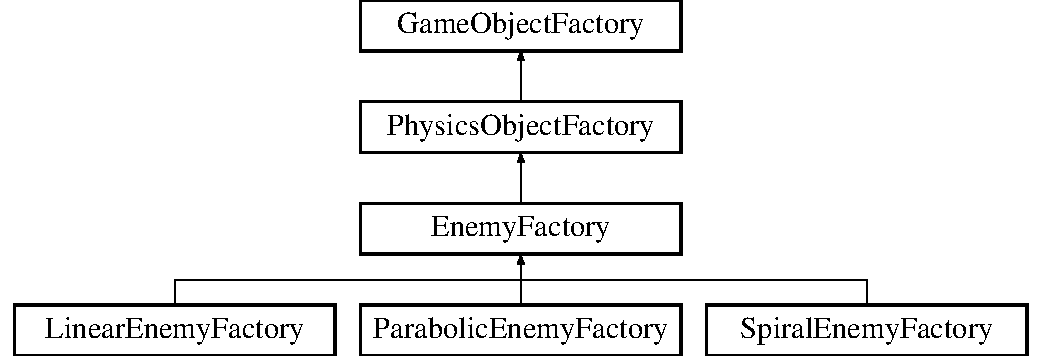
\includegraphics[height=4.000000cm]{d8/d4c/class_enemy_factory}
\end{center}
\end{figure}
\subsection*{Public Member Functions}
\begin{DoxyCompactItemize}
\item 
virtual std\+::shared\+\_\+ptr$<$ \hyperlink{class_game_object}{Game\+Object} $>$ \hyperlink{class_enemy_factory_acb6ad18d5ef69a27927907fa9a444c7d}{get\+Game\+Object} (const std\+::shared\+\_\+ptr$<$ \hyperlink{class_database_interface}{Database\+Interface} $>$ \&database) final
\begin{DoxyCompactList}\small\item\em Function call used to create an \hyperlink{class_enemy}{Enemy} Object. \end{DoxyCompactList}\item 
virtual std\+::shared\+\_\+ptr$<$ \hyperlink{class_movable_interface}{Movable\+Interface} $>$ \hyperlink{class_enemy_factory_ae064082d650e676960cb84ebb60ba216}{get\+Movable\+Type} (const \hyperlink{struct_game_object_data}{Game\+Object\+Data} \&data)=0
\begin{DoxyCompactList}\small\item\em Pure virtual function used to assign the various Movable\+Interfaces that the Enemy\+Objects use. \end{DoxyCompactList}\end{DoxyCompactItemize}


\subsection{Detailed Description}
\hyperlink{class_enemy}{Enemy} Factory is the base class to the various types of enemies that are constructed. 

\subsection{Member Function Documentation}
\mbox{\Hypertarget{class_enemy_factory_acb6ad18d5ef69a27927907fa9a444c7d}\label{class_enemy_factory_acb6ad18d5ef69a27927907fa9a444c7d}} 
\index{Enemy\+Factory@{Enemy\+Factory}!get\+Game\+Object@{get\+Game\+Object}}
\index{get\+Game\+Object@{get\+Game\+Object}!Enemy\+Factory@{Enemy\+Factory}}
\subsubsection{\texorpdfstring{get\+Game\+Object()}{getGameObject()}}
{\footnotesize\ttfamily std\+::shared\+\_\+ptr$<$ \hyperlink{class_game_object}{Game\+Object} $>$ Enemy\+Factory\+::get\+Game\+Object (\begin{DoxyParamCaption}\item[{const std\+::shared\+\_\+ptr$<$ \hyperlink{class_database_interface}{Database\+Interface} $>$ \&}]{database }\end{DoxyParamCaption})\hspace{0.3cm}{\ttfamily [final]}, {\ttfamily [virtual]}}



Function call used to create an \hyperlink{class_enemy}{Enemy} Object. 

\begin{DoxyReturn}{Returns}
Returns an \hyperlink{class_enemy}{Enemy} Object with the specific characteristics for this game
\end{DoxyReturn}
Creates the required parameters for each object and passes them by value to ensure that the information is copied to the object This is done so that the default object information is not changed. 

Reimplemented from \hyperlink{class_physics_object_factory_a2644107d0c455c3307559cd824a7c9a8}{Physics\+Object\+Factory}.

\mbox{\Hypertarget{class_enemy_factory_ae064082d650e676960cb84ebb60ba216}\label{class_enemy_factory_ae064082d650e676960cb84ebb60ba216}} 
\index{Enemy\+Factory@{Enemy\+Factory}!get\+Movable\+Type@{get\+Movable\+Type}}
\index{get\+Movable\+Type@{get\+Movable\+Type}!Enemy\+Factory@{Enemy\+Factory}}
\subsubsection{\texorpdfstring{get\+Movable\+Type()}{getMovableType()}}
{\footnotesize\ttfamily virtual std\+::shared\+\_\+ptr$<$\hyperlink{class_movable_interface}{Movable\+Interface}$>$ Enemy\+Factory\+::get\+Movable\+Type (\begin{DoxyParamCaption}\item[{const \hyperlink{struct_game_object_data}{Game\+Object\+Data} \&}]{data }\end{DoxyParamCaption})\hspace{0.3cm}{\ttfamily [pure virtual]}}



Pure virtual function used to assign the various Movable\+Interfaces that the Enemy\+Objects use. 


\begin{DoxyParams}{Parameters}
{\em data} & The \hyperlink{struct_game_object_data}{Game\+Object\+Data} specific to the \hyperlink{class_enemy}{Enemy} being constructed \\
\hline
\end{DoxyParams}
\begin{DoxyReturn}{Returns}
Returns the \hyperlink{class_movable_interface}{Movable\+Interface} for the specific \hyperlink{class_enemy}{Enemy} that is being constructed 
\end{DoxyReturn}


Implemented in \hyperlink{class_parabolic_enemy_factory_aaf1f3323e4c723f669a11c20a7e38efe}{Parabolic\+Enemy\+Factory}, \hyperlink{class_spiral_enemy_factory_aa05ff998b19ec4ef7ddd86ff24f70cba}{Spiral\+Enemy\+Factory}, and \hyperlink{class_linear_enemy_factory_ad8b2931b7f31f9f8e13d3c9d804469bf}{Linear\+Enemy\+Factory}.



The documentation for this class was generated from the following files\+:\begin{DoxyCompactItemize}
\item 
D\+:/\+Users/\+Tim-\/\+P\+C/\+Documents/\+Software\+\_\+\+I\+I/\+Project/\+Project\+Files/game-\/source-\/code/\+Back\+End\+Systems/Enemy\+Factory.\+h\item 
D\+:/\+Users/\+Tim-\/\+P\+C/\+Documents/\+Software\+\_\+\+I\+I/\+Project/\+Project\+Files/game-\/source-\/code/\+Back\+End\+Systems/Enemy\+Factory.\+cpp\end{DoxyCompactItemize}

\hypertarget{class_enemy_projectile}{}\section{Enemy\+Projectile Class Reference}
\label{class_enemy_projectile}\index{Enemy\+Projectile@{Enemy\+Projectile}}


Used to represent the enemy projectile and how it interacts with the various objects.  




{\ttfamily \#include $<$Enemy\+Projectile.\+h$>$}

Inheritance diagram for Enemy\+Projectile\+:\begin{figure}[H]
\begin{center}
\leavevmode
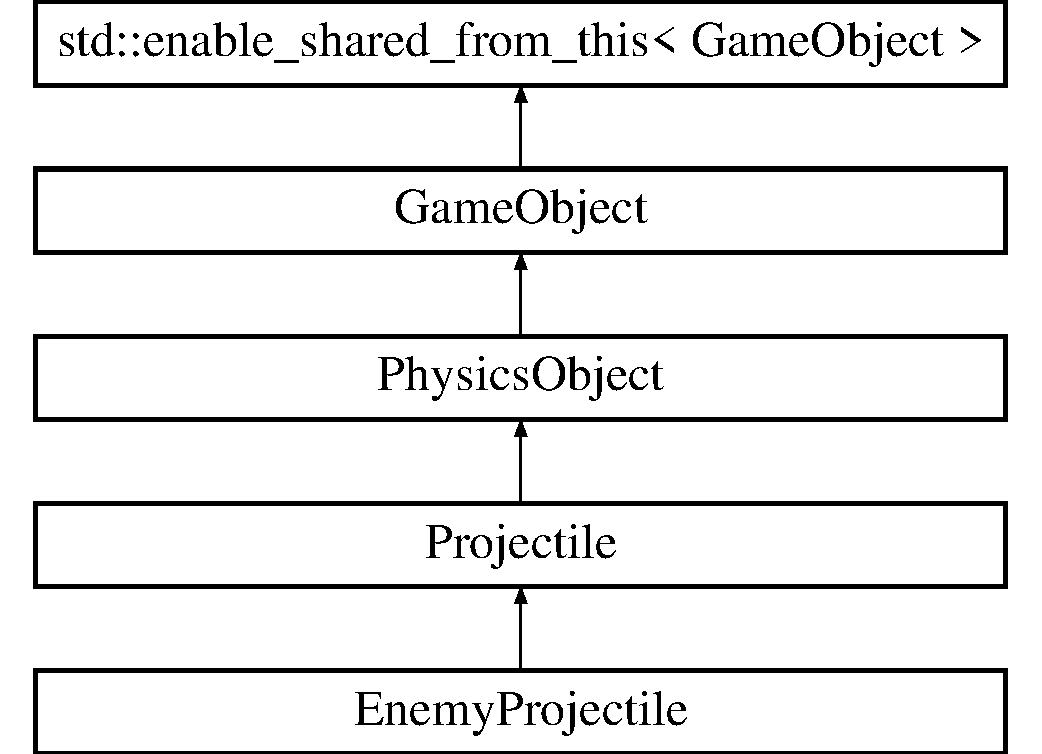
\includegraphics[height=5.000000cm]{da/db2/class_enemy_projectile}
\end{center}
\end{figure}
\subsection*{Public Member Functions}
\begin{DoxyCompactItemize}
\item 
\hyperlink{class_enemy_projectile_ab7040bb69b995ade3a18badb5486f0bb}{Enemy\+Projectile} (const \hyperlink{class_physics_object}{Physics\+Object} \&physics\+Object, const std\+::shared\+\_\+ptr$<$ \hyperlink{class_movable_interface}{Movable\+Interface} $>$ \&move, const \hyperlink{class_boundary}{Boundary} \&destroy\+Bounds)
\begin{DoxyCompactList}\small\item\em Constructs the \hyperlink{class_enemy}{Enemy} \hyperlink{class_projectile}{Projectile} object. \end{DoxyCompactList}\item 
\mbox{\Hypertarget{class_enemy_projectile_a6ea9e3418fd05ca7ecee016019206f70}\label{class_enemy_projectile_a6ea9e3418fd05ca7ecee016019206f70}} 
virtual void \hyperlink{class_enemy_projectile_a6ea9e3418fd05ca7ecee016019206f70}{Destroy\+Self} () override
\begin{DoxyCompactList}\small\item\em Object destroys itself when the object goes outside of the specified boundary. \end{DoxyCompactList}\item 
virtual void \hyperlink{class_enemy_projectile_a4b3233a5ba7a3df66070cd6cdaa0362a}{collision\+Action} (const Game\+Object\+Type \&object\+Type) override
\begin{DoxyCompactList}\small\item\em Response to colliding with the various objects within the game. \end{DoxyCompactList}\end{DoxyCompactItemize}
\subsection*{Additional Inherited Members}


\subsection{Detailed Description}
Used to represent the enemy projectile and how it interacts with the various objects. 

The template design pattern is used to create the \hyperlink{class_enemy_projectile}{Enemy\+Projectile} from the base \hyperlink{class_projectile}{Projectile} object so that only the most necessary functions are overriden to vary the \hyperlink{class_player_projectile}{Player\+Projectile} and the \hyperlink{class_enemy_projectile}{Enemy\+Projectile} 

\subsection{Constructor \& Destructor Documentation}
\mbox{\Hypertarget{class_enemy_projectile_ab7040bb69b995ade3a18badb5486f0bb}\label{class_enemy_projectile_ab7040bb69b995ade3a18badb5486f0bb}} 
\index{Enemy\+Projectile@{Enemy\+Projectile}!Enemy\+Projectile@{Enemy\+Projectile}}
\index{Enemy\+Projectile@{Enemy\+Projectile}!Enemy\+Projectile@{Enemy\+Projectile}}
\subsubsection{\texorpdfstring{Enemy\+Projectile()}{EnemyProjectile()}}
{\footnotesize\ttfamily Enemy\+Projectile\+::\+Enemy\+Projectile (\begin{DoxyParamCaption}\item[{const \hyperlink{class_physics_object}{Physics\+Object} \&}]{physics\+Object,  }\item[{const std\+::shared\+\_\+ptr$<$ \hyperlink{class_movable_interface}{Movable\+Interface} $>$ \&}]{move,  }\item[{const \hyperlink{class_boundary}{Boundary} \&}]{destroy\+Bounds }\end{DoxyParamCaption})}



Constructs the \hyperlink{class_enemy}{Enemy} \hyperlink{class_projectile}{Projectile} object. 


\begin{DoxyParams}{Parameters}
{\em physics\+Object} & Assigns the properties of the Physics object to the \hyperlink{class_enemy_projectile}{Enemy\+Projectile} constructed \\
\hline
{\em move} & Move\+Interface used by the \hyperlink{class_enemy_projectile}{Enemy\+Projectile} \\
\hline
{\em destroy\+Bounds} & \hyperlink{class_boundary}{Boundary} for which the object exists inside \\
\hline
\end{DoxyParams}


\subsection{Member Function Documentation}
\mbox{\Hypertarget{class_enemy_projectile_a4b3233a5ba7a3df66070cd6cdaa0362a}\label{class_enemy_projectile_a4b3233a5ba7a3df66070cd6cdaa0362a}} 
\index{Enemy\+Projectile@{Enemy\+Projectile}!collision\+Action@{collision\+Action}}
\index{collision\+Action@{collision\+Action}!Enemy\+Projectile@{Enemy\+Projectile}}
\subsubsection{\texorpdfstring{collision\+Action()}{collisionAction()}}
{\footnotesize\ttfamily void Enemy\+Projectile\+::collision\+Action (\begin{DoxyParamCaption}\item[{const Game\+Object\+Type \&}]{object\+Type }\end{DoxyParamCaption})\hspace{0.3cm}{\ttfamily [override]}, {\ttfamily [virtual]}}



Response to colliding with the various objects within the game. 


\begin{DoxyParams}{Parameters}
{\em object\+Type} & The type of object that has collided with the current \hyperlink{class_enemy_projectile}{Enemy\+Projectile} \\
\hline
\end{DoxyParams}


Reimplemented from \hyperlink{class_physics_object_a16163f4e5bf781b3814d024c9f44a276}{Physics\+Object}.



The documentation for this class was generated from the following files\+:\begin{DoxyCompactItemize}
\item 
D\+:/\+Users/\+Tim-\/\+P\+C/\+Documents/\+Software\+\_\+\+I\+I/\+Project/\+Project\+Files/game-\/source-\/code/\+Front\+End\+Systems/Enemy\+Projectile.\+h\item 
D\+:/\+Users/\+Tim-\/\+P\+C/\+Documents/\+Software\+\_\+\+I\+I/\+Project/\+Project\+Files/game-\/source-\/code/\+Front\+End\+Systems/Enemy\+Projectile.\+cpp\end{DoxyCompactItemize}

\hypertarget{class_enemy_projectile_factory}{}\section{Enemy\+Projectile\+Factory Class Reference}
\label{class_enemy_projectile_factory}\index{Enemy\+Projectile\+Factory@{Enemy\+Projectile\+Factory}}


\hyperlink{class_enemy_controller_factory}{Enemy\+Controller\+Factory} is responsible for the construction of any \hyperlink{class_enemy_controller}{Enemy\+Controller} objects.  




{\ttfamily \#include $<$Enemy\+Projectile\+Factory.\+h$>$}

Inheritance diagram for Enemy\+Projectile\+Factory\+:\begin{figure}[H]
\begin{center}
\leavevmode
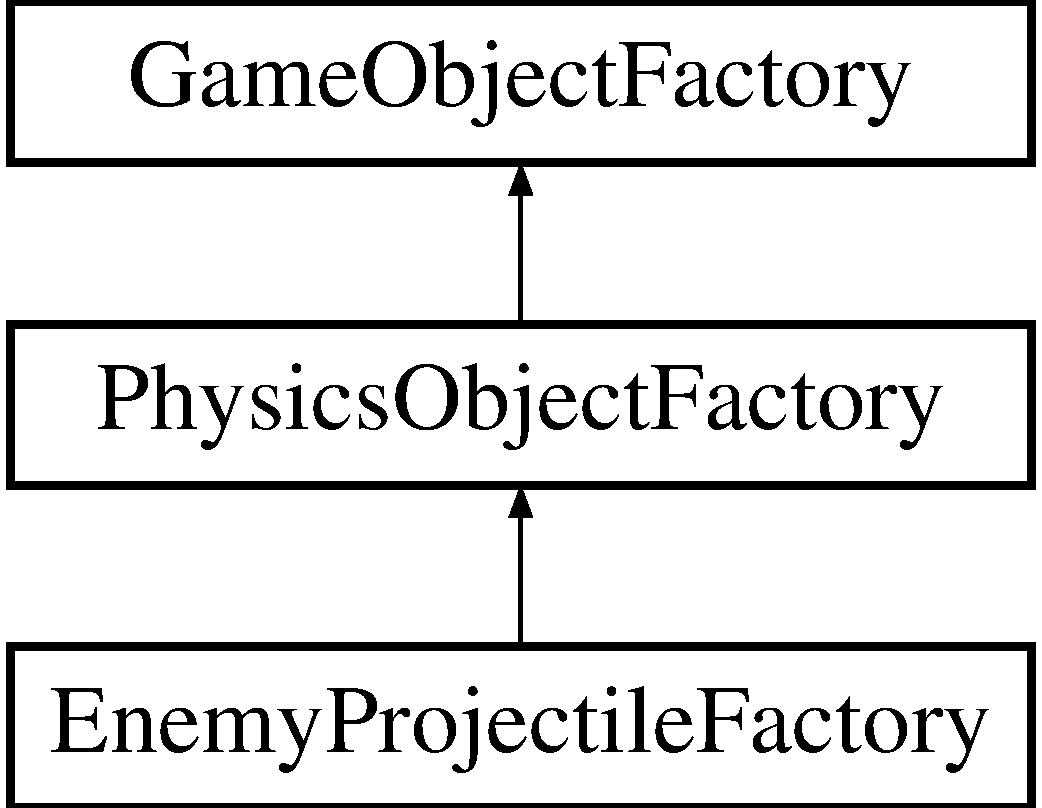
\includegraphics[height=3.000000cm]{d2/db0/class_enemy_projectile_factory}
\end{center}
\end{figure}
\subsection*{Public Member Functions}
\begin{DoxyCompactItemize}
\item 
virtual std\+::shared\+\_\+ptr$<$ \hyperlink{class_game_object}{Game\+Object} $>$ \hyperlink{class_enemy_projectile_factory_a081c6bea7032956c278fdf4ff62d530a}{get\+Game\+Object} (const std\+::shared\+\_\+ptr$<$ \hyperlink{class_database_interface}{Database\+Interface} $>$ \&database) override
\begin{DoxyCompactList}\small\item\em Function call used to create an \hyperlink{class_enemy_projectile}{Enemy\+Projectile} Object. \end{DoxyCompactList}\item 
virtual \hyperlink{struct_game_object_data}{Game\+Object\+Data} \hyperlink{class_enemy_projectile_factory_a1ef660e5962f29b7353054c6480477c7}{get\+Object\+Data} (const std\+::shared\+\_\+ptr$<$ \hyperlink{class_database_interface}{Database\+Interface} $>$ \&database) override
\begin{DoxyCompactList}\small\item\em used to obtain the specific \hyperlink{struct_game_object_data}{Game\+Object\+Data} defined for the current factory \end{DoxyCompactList}\end{DoxyCompactItemize}


\subsection{Detailed Description}
\hyperlink{class_enemy_controller_factory}{Enemy\+Controller\+Factory} is responsible for the construction of any \hyperlink{class_enemy_controller}{Enemy\+Controller} objects. 

\subsection{Member Function Documentation}
\mbox{\Hypertarget{class_enemy_projectile_factory_a081c6bea7032956c278fdf4ff62d530a}\label{class_enemy_projectile_factory_a081c6bea7032956c278fdf4ff62d530a}} 
\index{Enemy\+Projectile\+Factory@{Enemy\+Projectile\+Factory}!get\+Game\+Object@{get\+Game\+Object}}
\index{get\+Game\+Object@{get\+Game\+Object}!Enemy\+Projectile\+Factory@{Enemy\+Projectile\+Factory}}
\subsubsection{\texorpdfstring{get\+Game\+Object()}{getGameObject()}}
{\footnotesize\ttfamily std\+::shared\+\_\+ptr$<$ \hyperlink{class_game_object}{Game\+Object} $>$ Enemy\+Projectile\+Factory\+::get\+Game\+Object (\begin{DoxyParamCaption}\item[{const std\+::shared\+\_\+ptr$<$ \hyperlink{class_database_interface}{Database\+Interface} $>$ \&}]{database }\end{DoxyParamCaption})\hspace{0.3cm}{\ttfamily [override]}, {\ttfamily [virtual]}}



Function call used to create an \hyperlink{class_enemy_projectile}{Enemy\+Projectile} Object. 

\begin{DoxyReturn}{Returns}
Returns an An \hyperlink{class_enemy_projectile}{Enemy\+Projectile} Object with the specific characteristics for this game 
\end{DoxyReturn}


Reimplemented from \hyperlink{class_physics_object_factory_a2644107d0c455c3307559cd824a7c9a8}{Physics\+Object\+Factory}.

\mbox{\Hypertarget{class_enemy_projectile_factory_a1ef660e5962f29b7353054c6480477c7}\label{class_enemy_projectile_factory_a1ef660e5962f29b7353054c6480477c7}} 
\index{Enemy\+Projectile\+Factory@{Enemy\+Projectile\+Factory}!get\+Object\+Data@{get\+Object\+Data}}
\index{get\+Object\+Data@{get\+Object\+Data}!Enemy\+Projectile\+Factory@{Enemy\+Projectile\+Factory}}
\subsubsection{\texorpdfstring{get\+Object\+Data()}{getObjectData()}}
{\footnotesize\ttfamily \hyperlink{struct_game_object_data}{Game\+Object\+Data} Enemy\+Projectile\+Factory\+::get\+Object\+Data (\begin{DoxyParamCaption}\item[{const std\+::shared\+\_\+ptr$<$ \hyperlink{class_database_interface}{Database\+Interface} $>$ \&}]{database }\end{DoxyParamCaption})\hspace{0.3cm}{\ttfamily [override]}, {\ttfamily [virtual]}}



used to obtain the specific \hyperlink{struct_game_object_data}{Game\+Object\+Data} defined for the current factory 


\begin{DoxyParams}{Parameters}
{\em database} & The specific \hyperlink{class_database_interface}{Database\+Interface} that contains the information about the \hyperlink{class_game_object}{Game\+Object} \\
\hline
\end{DoxyParams}
\begin{DoxyReturn}{Returns}
The \hyperlink{struct_game_object_data}{Game\+Object\+Data} required for the construction of the object 
\end{DoxyReturn}


Implements \hyperlink{class_physics_object_factory_aa59f52d3adc1fac676f4a8a3c2de9ba9}{Physics\+Object\+Factory}.



The documentation for this class was generated from the following files\+:\begin{DoxyCompactItemize}
\item 
C\+:/\+Users/\+Tim/\+Documents/\+Software\+Dev/\+Software\+Project/\+Project\+Files/game-\/source-\/code/\+Back\+End\+Systems/Enemy\+Projectile\+Factory.\+h\item 
C\+:/\+Users/\+Tim/\+Documents/\+Software\+Dev/\+Software\+Project/\+Project\+Files/game-\/source-\/code/\+Back\+End\+Systems/Enemy\+Projectile\+Factory.\+cpp\end{DoxyCompactItemize}

\hypertarget{class_event_manager}{}\section{Event\+Manager Class Reference}
\label{class_event_manager}\index{Event\+Manager@{Event\+Manager}}


can be converted into a singleton  




{\ttfamily \#include $<$Event\+Manager.\+h$>$}

\subsection*{Public Member Functions}
\begin{DoxyCompactItemize}
\item 
\mbox{\Hypertarget{class_event_manager_a89099b22114f158b5c530edfea52371d}\label{class_event_manager_a89099b22114f158b5c530edfea52371d}} 
\hyperlink{class_event_manager_a89099b22114f158b5c530edfea52371d}{Event\+Manager} ()
\begin{DoxyCompactList}\small\item\em redundant constructors should be removed, only a default is necessary with the event loop function \end{DoxyCompactList}\item 
\mbox{\Hypertarget{class_event_manager_a8951d1cf3aabe678cd37c64317497519}\label{class_event_manager_a8951d1cf3aabe678cd37c64317497519}} 
{\bfseries Event\+Manager} (Render\+Window $\ast$event\+Window)
\item 
\mbox{\Hypertarget{class_event_manager_a3e90c3658f1fc88b45ba1b8fda4f2c10}\label{class_event_manager_a3e90c3658f1fc88b45ba1b8fda4f2c10}} 
void {\bfseries Event\+Loop} (Render\+Window \&event\+Window)
\end{DoxyCompactItemize}
\subsection*{Private Member Functions}
\begin{DoxyCompactItemize}
\item 
\mbox{\Hypertarget{class_event_manager_a279b1d4e14cd98c1b3789a5276be2b3a}\label{class_event_manager_a279b1d4e14cd98c1b3789a5276be2b3a}} 
void {\bfseries Key\+Input} (const Event \&event, bool state)
\end{DoxyCompactItemize}
\subsection*{Private Attributes}
\begin{DoxyCompactItemize}
\item 
\mbox{\Hypertarget{class_event_manager_a1909a88890831dfd326b4a9032c48ac2}\label{class_event_manager_a1909a88890831dfd326b4a9032c48ac2}} 
std\+::shared\+\_\+ptr$<$ Render\+Window $>$ \hyperlink{class_event_manager_a1909a88890831dfd326b4a9032c48ac2}{\+\_\+event\+Window}
\begin{DoxyCompactList}\small\item\em redundant shared pointer \end{DoxyCompactList}\end{DoxyCompactItemize}


\subsection{Detailed Description}
can be converted into a singleton 

The documentation for this class was generated from the following files\+:\begin{DoxyCompactItemize}
\item 
D\+:/\+Users/\+Tim-\/\+P\+C/\+Documents/\+Software\+\_\+\+I\+I/\+Project/\+Project\+Files/game-\/source-\/code/\+Back\+End\+Systems/Event\+Manager.\+h\item 
D\+:/\+Users/\+Tim-\/\+P\+C/\+Documents/\+Software\+\_\+\+I\+I/\+Project/\+Project\+Files/game-\/source-\/code/\+Back\+End\+Systems/Event\+Manager.\+cpp\end{DoxyCompactItemize}

\hypertarget{class_failed_to_load_texture}{}\section{Failed\+To\+Load\+Texture Class Reference}
\label{class_failed_to_load_texture}\index{Failed\+To\+Load\+Texture@{Failed\+To\+Load\+Texture}}


The documentation for this class was generated from the following file\+:\begin{DoxyCompactItemize}
\item 
D\+:/\+Users/\+Tim-\/\+P\+C/\+Documents/\+Software\+\_\+\+I\+I/\+Project/\+Project\+Files/game-\/source-\/code/\+Back\+End\+Systems/Display\+Manger.\+cpp\end{DoxyCompactItemize}

\hypertarget{class_file_cannot_be_opened}{}\section{File\+Cannot\+Be\+Opened Class Reference}
\label{class_file_cannot_be_opened}\index{File\+Cannot\+Be\+Opened@{File\+Cannot\+Be\+Opened}}


Exception thrown if the file inputed cannot be opened.  




{\ttfamily \#include $<$Read\+From\+File.\+h$>$}



\subsection{Detailed Description}
Exception thrown if the file inputed cannot be opened. 

The documentation for this class was generated from the following file\+:\begin{DoxyCompactItemize}
\item 
D\+:/\+Users/\+Tim-\/\+P\+C/\+Documents/\+Software\+\_\+\+I\+I/\+Project/\+Project\+Files/game-\/source-\/code/\+Back\+End\+Systems/Read\+From\+File.\+h\end{DoxyCompactItemize}

\hypertarget{class_game_manager}{}\section{Game\+Manager Class Reference}
\label{class_game_manager}\index{Game\+Manager@{Game\+Manager}}


\hyperlink{class_game_manager}{Game\+Manager} is responsible for intialising and maintaining the game state, and updating the game loop through the composition of different \hyperlink{class_scene}{Scene} objects that exist within the game, it communicates with the \hyperlink{class_event_manager}{Event\+Manager}, \hyperlink{class_display_manager}{Display\+Manager} and \hyperlink{class_collision_detection}{Collision\+Detection} classes regarding the state of the game.  




{\ttfamily \#include $<$Game\+Manager.\+h$>$}

\subsection*{Public Member Functions}
\begin{DoxyCompactItemize}
\item 
\hyperlink{class_game_manager_a05f6a37de95fcea1313fe4476b95941d}{Game\+Manager} (std\+::shared\+\_\+ptr$<$ \hyperlink{class_repositiory_interface}{Repositiory\+Interface} $>$ repository)
\begin{DoxyCompactList}\small\item\em Constructs the \hyperlink{class_game_manager}{Game\+Manager} object neccesary for the Game loop. \end{DoxyCompactList}\item 
\mbox{\Hypertarget{class_game_manager_a5baa570812ae717f809fe0dc48bde22e}\label{class_game_manager_a5baa570812ae717f809fe0dc48bde22e}} 
void \hyperlink{class_game_manager_a5baa570812ae717f809fe0dc48bde22e}{Game\+Loop} ()
\begin{DoxyCompactList}\small\item\em Runs the main game loop of the game, and updates the various Game\+Objects Stored inside of the active\+Scene. \end{DoxyCompactList}\item 
void \hyperlink{class_game_manager_a09b8801bcfdd8d5cbc52e27895b84e3b}{Load\+Scene} (unsigned int index)
\begin{DoxyCompactList}\small\item\em Changes the active \hyperlink{class_scene}{Scene} to the \hyperlink{class_scene}{Scene} at the desired Scene\+Index. \end{DoxyCompactList}\end{DoxyCompactItemize}
\subsection*{Static Public Member Functions}
\begin{DoxyCompactItemize}
\item 
static void \hyperlink{class_game_manager_acbd9fb84f9e18c8cb585738d5c89a2b9}{Exit} ()
\begin{DoxyCompactList}\small\item\em Closes the game window. \end{DoxyCompactList}\item 
static int \hyperlink{class_game_manager_aa4835b5fc96bfdbf6170a8673baf5552}{get\+Scene\+Index} ()
\begin{DoxyCompactList}\small\item\em Returns the current scene index. \end{DoxyCompactList}\item 
static const bool \hyperlink{class_game_manager_a4eb94c6171bf3292eb57b291e2174289}{game\+Closed} ()
\begin{DoxyCompactList}\small\item\em Identifies whether the game has been closed. \end{DoxyCompactList}\end{DoxyCompactItemize}
\subsection*{Static Public Attributes}
\begin{DoxyCompactItemize}
\item 
static std\+::shared\+\_\+ptr$<$ \hyperlink{class_scene}{Scene} $>$ \hyperlink{class_game_manager_a969dd909c6b70310843d34e2490736b4}{active\+Scene} = N\+U\+LL
\end{DoxyCompactItemize}
\subsection*{Private Member Functions}
\begin{DoxyCompactItemize}
\item 
void \hyperlink{class_game_manager_a0a4c03ef0451371a98204c18c1faf9fd}{initialise\+Window} (sf\+::\+Render\+Window \&\+\_\+game\+Window)
\begin{DoxyCompactList}\small\item\em Initialises the sfml Render\+Window to the properties defined by the default window settings. \end{DoxyCompactList}\end{DoxyCompactItemize}
\subsection*{Private Attributes}
\begin{DoxyCompactItemize}
\item 
std\+::shared\+\_\+ptr$<$ \hyperlink{class_repositiory_interface}{Repositiory\+Interface} $>$ \hyperlink{class_game_manager_adf8ffad3969c2bee2332eb3ea58a3c9c}{\+\_\+repository}
\item 
sf\+::\+Render\+Window \hyperlink{class_game_manager_a0c91609e7557e4e97a0e4be541254a38}{\+\_\+window}
\item 
std\+::unique\+\_\+ptr$<$ \hyperlink{class_game_time}{Game\+Time} $>$ \hyperlink{class_game_manager_ae08fe7df616e789e4858645b56d9b73b}{\+\_\+game\+Time}
\item 
\hyperlink{struct_window_settings}{Window\+Settings} \hyperlink{class_game_manager_a06843f28cb1609e41da7eee19be9aa87}{\+\_\+default\+Setup}
\item 
std\+::vector$<$ std\+::shared\+\_\+ptr$<$ \hyperlink{class_scene}{Scene} $>$ $>$ \hyperlink{class_game_manager_a6be6c6b38c1b95d7fd84819eba50e618}{\+\_\+game\+\_\+scenes}
\end{DoxyCompactItemize}
\subsection*{Static Private Attributes}
\begin{DoxyCompactItemize}
\item 
static int \hyperlink{class_game_manager_aedb575ca538853f3d7053b33bef238e0}{\+\_\+scene\+\_\+index} = 0
\item 
static bool \hyperlink{class_game_manager_a07c75a9507a0d82f88a0b62d808fcf3c}{close\+Window} = false
\end{DoxyCompactItemize}


\subsection{Detailed Description}
\hyperlink{class_game_manager}{Game\+Manager} is responsible for intialising and maintaining the game state, and updating the game loop through the composition of different \hyperlink{class_scene}{Scene} objects that exist within the game, it communicates with the \hyperlink{class_event_manager}{Event\+Manager}, \hyperlink{class_display_manager}{Display\+Manager} and \hyperlink{class_collision_detection}{Collision\+Detection} classes regarding the state of the game. 

\subsection{Constructor \& Destructor Documentation}
\mbox{\Hypertarget{class_game_manager_a05f6a37de95fcea1313fe4476b95941d}\label{class_game_manager_a05f6a37de95fcea1313fe4476b95941d}} 
\index{Game\+Manager@{Game\+Manager}!Game\+Manager@{Game\+Manager}}
\index{Game\+Manager@{Game\+Manager}!Game\+Manager@{Game\+Manager}}
\subsubsection{\texorpdfstring{Game\+Manager()}{GameManager()}}
{\footnotesize\ttfamily Game\+Manager\+::\+Game\+Manager (\begin{DoxyParamCaption}\item[{std\+::shared\+\_\+ptr$<$ \hyperlink{class_repositiory_interface}{Repositiory\+Interface} $>$}]{repository }\end{DoxyParamCaption})}



Constructs the \hyperlink{class_game_manager}{Game\+Manager} object neccesary for the Game loop. 


\begin{DoxyParams}{Parameters}
{\em repository} & The instance of the \hyperlink{class_repository}{Repository} used to generate the Scenes for the game \\
\hline
\end{DoxyParams}


\subsection{Member Function Documentation}
\mbox{\Hypertarget{class_game_manager_acbd9fb84f9e18c8cb585738d5c89a2b9}\label{class_game_manager_acbd9fb84f9e18c8cb585738d5c89a2b9}} 
\index{Game\+Manager@{Game\+Manager}!Exit@{Exit}}
\index{Exit@{Exit}!Game\+Manager@{Game\+Manager}}
\subsubsection{\texorpdfstring{Exit()}{Exit()}}
{\footnotesize\ttfamily void Game\+Manager\+::\+Exit (\begin{DoxyParamCaption}{ }\end{DoxyParamCaption})\hspace{0.3cm}{\ttfamily [static]}}



Closes the game window. 

Exit function needs to be moved into \hyperlink{class_scene}{Scene} or a seperate \hyperlink{class_application}{Application} class. \mbox{\Hypertarget{class_game_manager_a4eb94c6171bf3292eb57b291e2174289}\label{class_game_manager_a4eb94c6171bf3292eb57b291e2174289}} 
\index{Game\+Manager@{Game\+Manager}!game\+Closed@{game\+Closed}}
\index{game\+Closed@{game\+Closed}!Game\+Manager@{Game\+Manager}}
\subsubsection{\texorpdfstring{game\+Closed()}{gameClosed()}}
{\footnotesize\ttfamily static const bool Game\+Manager\+::game\+Closed (\begin{DoxyParamCaption}{ }\end{DoxyParamCaption})\hspace{0.3cm}{\ttfamily [inline]}, {\ttfamily [static]}}



Identifies whether the game has been closed. 

\begin{DoxyReturn}{Returns}
Returns a constant bool whether the game is closed 
\end{DoxyReturn}
\mbox{\Hypertarget{class_game_manager_aa4835b5fc96bfdbf6170a8673baf5552}\label{class_game_manager_aa4835b5fc96bfdbf6170a8673baf5552}} 
\index{Game\+Manager@{Game\+Manager}!get\+Scene\+Index@{get\+Scene\+Index}}
\index{get\+Scene\+Index@{get\+Scene\+Index}!Game\+Manager@{Game\+Manager}}
\subsubsection{\texorpdfstring{get\+Scene\+Index()}{getSceneIndex()}}
{\footnotesize\ttfamily static int Game\+Manager\+::get\+Scene\+Index (\begin{DoxyParamCaption}{ }\end{DoxyParamCaption})\hspace{0.3cm}{\ttfamily [inline]}, {\ttfamily [static]}}



Returns the current scene index. 

\begin{DoxyReturn}{Returns}
The Current \hyperlink{class_scene}{Scene} Index 
\end{DoxyReturn}
\mbox{\Hypertarget{class_game_manager_a0a4c03ef0451371a98204c18c1faf9fd}\label{class_game_manager_a0a4c03ef0451371a98204c18c1faf9fd}} 
\index{Game\+Manager@{Game\+Manager}!initialise\+Window@{initialise\+Window}}
\index{initialise\+Window@{initialise\+Window}!Game\+Manager@{Game\+Manager}}
\subsubsection{\texorpdfstring{initialise\+Window()}{initialiseWindow()}}
{\footnotesize\ttfamily void Game\+Manager\+::initialise\+Window (\begin{DoxyParamCaption}\item[{sf\+::\+Render\+Window \&}]{\+\_\+game\+Window }\end{DoxyParamCaption})\hspace{0.3cm}{\ttfamily [private]}}



Initialises the sfml Render\+Window to the properties defined by the default window settings. 


\begin{DoxyParams}{Parameters}
{\em \+\_\+game\+Window} & \\
\hline
\end{DoxyParams}
\mbox{\Hypertarget{class_game_manager_a09b8801bcfdd8d5cbc52e27895b84e3b}\label{class_game_manager_a09b8801bcfdd8d5cbc52e27895b84e3b}} 
\index{Game\+Manager@{Game\+Manager}!Load\+Scene@{Load\+Scene}}
\index{Load\+Scene@{Load\+Scene}!Game\+Manager@{Game\+Manager}}
\subsubsection{\texorpdfstring{Load\+Scene()}{LoadScene()}}
{\footnotesize\ttfamily void Game\+Manager\+::\+Load\+Scene (\begin{DoxyParamCaption}\item[{unsigned int}]{index }\end{DoxyParamCaption})}



Changes the active \hyperlink{class_scene}{Scene} to the \hyperlink{class_scene}{Scene} at the desired Scene\+Index. 

Should be called from an application class but remains inside of game\+Manager.


\begin{DoxyParams}{Parameters}
{\em index} & The index for which the desired scene is located \\
\hline
\end{DoxyParams}


\subsection{Member Data Documentation}
\mbox{\Hypertarget{class_game_manager_a06843f28cb1609e41da7eee19be9aa87}\label{class_game_manager_a06843f28cb1609e41da7eee19be9aa87}} 
\index{Game\+Manager@{Game\+Manager}!\+\_\+default\+Setup@{\+\_\+default\+Setup}}
\index{\+\_\+default\+Setup@{\+\_\+default\+Setup}!Game\+Manager@{Game\+Manager}}
\subsubsection{\texorpdfstring{\+\_\+default\+Setup}{\_defaultSetup}}
{\footnotesize\ttfamily \hyperlink{struct_window_settings}{Window\+Settings} Game\+Manager\+::\+\_\+default\+Setup\hspace{0.3cm}{\ttfamily [private]}}

the default Setup information for the game \mbox{\Hypertarget{class_game_manager_a6be6c6b38c1b95d7fd84819eba50e618}\label{class_game_manager_a6be6c6b38c1b95d7fd84819eba50e618}} 
\index{Game\+Manager@{Game\+Manager}!\+\_\+game\+\_\+scenes@{\+\_\+game\+\_\+scenes}}
\index{\+\_\+game\+\_\+scenes@{\+\_\+game\+\_\+scenes}!Game\+Manager@{Game\+Manager}}
\subsubsection{\texorpdfstring{\+\_\+game\+\_\+scenes}{\_game\_scenes}}
{\footnotesize\ttfamily std\+::vector$<$std\+::shared\+\_\+ptr$<$\hyperlink{class_scene}{Scene}$>$ $>$ Game\+Manager\+::\+\_\+game\+\_\+scenes\hspace{0.3cm}{\ttfamily [private]}}

A vector of \hyperlink{class_scene}{Scene} Objects used to represent the different Scenes of the game \mbox{\Hypertarget{class_game_manager_ae08fe7df616e789e4858645b56d9b73b}\label{class_game_manager_ae08fe7df616e789e4858645b56d9b73b}} 
\index{Game\+Manager@{Game\+Manager}!\+\_\+game\+Time@{\+\_\+game\+Time}}
\index{\+\_\+game\+Time@{\+\_\+game\+Time}!Game\+Manager@{Game\+Manager}}
\subsubsection{\texorpdfstring{\+\_\+game\+Time}{\_gameTime}}
{\footnotesize\ttfamily std\+::unique\+\_\+ptr$<$\hyperlink{class_game_time}{Game\+Time}$>$ Game\+Manager\+::\+\_\+game\+Time\hspace{0.3cm}{\ttfamily [private]}}

A unique pointer to a \hyperlink{class_game_time}{Game\+Time} object, used to update the time between frames \mbox{\Hypertarget{class_game_manager_adf8ffad3969c2bee2332eb3ea58a3c9c}\label{class_game_manager_adf8ffad3969c2bee2332eb3ea58a3c9c}} 
\index{Game\+Manager@{Game\+Manager}!\+\_\+repository@{\+\_\+repository}}
\index{\+\_\+repository@{\+\_\+repository}!Game\+Manager@{Game\+Manager}}
\subsubsection{\texorpdfstring{\+\_\+repository}{\_repository}}
{\footnotesize\ttfamily std\+::shared\+\_\+ptr$<$\hyperlink{class_repositiory_interface}{Repositiory\+Interface}$>$ Game\+Manager\+::\+\_\+repository\hspace{0.3cm}{\ttfamily [private]}}

The Repository\+Interface used to generate the Scenes for the game \mbox{\Hypertarget{class_game_manager_aedb575ca538853f3d7053b33bef238e0}\label{class_game_manager_aedb575ca538853f3d7053b33bef238e0}} 
\index{Game\+Manager@{Game\+Manager}!\+\_\+scene\+\_\+index@{\+\_\+scene\+\_\+index}}
\index{\+\_\+scene\+\_\+index@{\+\_\+scene\+\_\+index}!Game\+Manager@{Game\+Manager}}
\subsubsection{\texorpdfstring{\+\_\+scene\+\_\+index}{\_scene\_index}}
{\footnotesize\ttfamily int Game\+Manager\+::\+\_\+scene\+\_\+index = 0\hspace{0.3cm}{\ttfamily [static]}, {\ttfamily [private]}}

The current \hyperlink{class_scene}{Scene} Index for the game \mbox{\Hypertarget{class_game_manager_a0c91609e7557e4e97a0e4be541254a38}\label{class_game_manager_a0c91609e7557e4e97a0e4be541254a38}} 
\index{Game\+Manager@{Game\+Manager}!\+\_\+window@{\+\_\+window}}
\index{\+\_\+window@{\+\_\+window}!Game\+Manager@{Game\+Manager}}
\subsubsection{\texorpdfstring{\+\_\+window}{\_window}}
{\footnotesize\ttfamily sf\+::\+Render\+Window Game\+Manager\+::\+\_\+window\hspace{0.3cm}{\ttfamily [private]}}

The sfml Render\+Window used for the game \mbox{\Hypertarget{class_game_manager_a969dd909c6b70310843d34e2490736b4}\label{class_game_manager_a969dd909c6b70310843d34e2490736b4}} 
\index{Game\+Manager@{Game\+Manager}!active\+Scene@{active\+Scene}}
\index{active\+Scene@{active\+Scene}!Game\+Manager@{Game\+Manager}}
\subsubsection{\texorpdfstring{active\+Scene}{activeScene}}
{\footnotesize\ttfamily std\+::shared\+\_\+ptr$<$ \hyperlink{class_scene}{Scene} $>$ Game\+Manager\+::active\+Scene = N\+U\+LL\hspace{0.3cm}{\ttfamily [static]}}

public static variable that represents the active \hyperlink{class_scene}{Scene} -\/ Bad design reveals too much information \mbox{\Hypertarget{class_game_manager_a07c75a9507a0d82f88a0b62d808fcf3c}\label{class_game_manager_a07c75a9507a0d82f88a0b62d808fcf3c}} 
\index{Game\+Manager@{Game\+Manager}!close\+Window@{close\+Window}}
\index{close\+Window@{close\+Window}!Game\+Manager@{Game\+Manager}}
\subsubsection{\texorpdfstring{close\+Window}{closeWindow}}
{\footnotesize\ttfamily bool Game\+Manager\+::close\+Window = false\hspace{0.3cm}{\ttfamily [static]}, {\ttfamily [private]}}

bool used to identify when the game should be closed 

The documentation for this class was generated from the following files\+:\begin{DoxyCompactItemize}
\item 
D\+:/\+Users/\+Tim-\/\+P\+C/\+Documents/\+Software\+\_\+\+I\+I/\+Project/\+Project\+Files/game-\/source-\/code/\+Back\+End\+Systems/Game\+Manager.\+h\item 
D\+:/\+Users/\+Tim-\/\+P\+C/\+Documents/\+Software\+\_\+\+I\+I/\+Project/\+Project\+Files/game-\/source-\/code/\+Back\+End\+Systems/Game\+Manager.\+cpp\end{DoxyCompactItemize}

\hypertarget{class_game_object}{}\section{Game\+Object Class Reference}
\label{class_game_object}\index{Game\+Object@{Game\+Object}}


The base class that is used for all game logic systems.  




{\ttfamily \#include $<$Game\+Object.\+h$>$}

Inheritance diagram for Game\+Object\+:\begin{figure}[H]
\begin{center}
\leavevmode
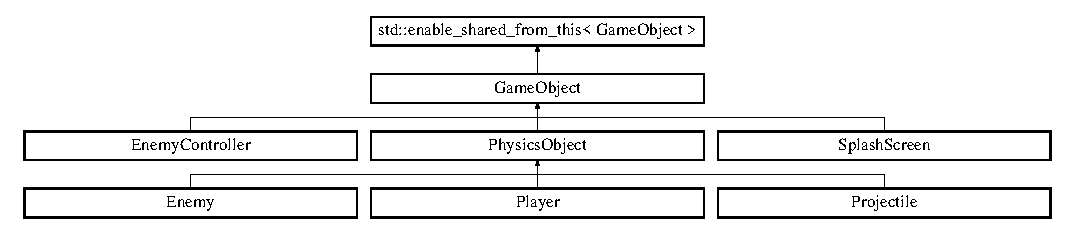
\includegraphics[height=2.021661cm]{d0/dd1/class_game_object}
\end{center}
\end{figure}
\subsection*{Public Member Functions}
\begin{DoxyCompactItemize}
\item 
\mbox{\Hypertarget{class_game_object_a0348e3ee2e83d56eafca7a3547f432c4}\label{class_game_object_a0348e3ee2e83d56eafca7a3547f432c4}} 
\hyperlink{class_game_object_a0348e3ee2e83d56eafca7a3547f432c4}{Game\+Object} ()
\begin{DoxyCompactList}\small\item\em Default Constructor -\/ Creates the object using default values. \end{DoxyCompactList}\item 
\hyperlink{class_game_object_a780db39d3dc5b54c4dffe2f429f9b656}{Game\+Object} (const \hyperlink{class_graphic_object}{Graphic\+Object} \&graphic)
\begin{DoxyCompactList}\small\item\em Constructs an object with a specific \hyperlink{class_graphic_object}{Graphic\+Object}. \end{DoxyCompactList}\item 
\hyperlink{class_game_object_a93186927c126a290592e3d7c13906f18}{Game\+Object} (const \hyperlink{structxy_vector}{xy\+Vector} \&scale)
\begin{DoxyCompactList}\small\item\em Constructs an object with a specific scale. \end{DoxyCompactList}\item 
\hyperlink{class_game_object_a8a9022df605afb6be63d0dcca07667d6}{Game\+Object} (const \hyperlink{class_vector2_d}{Vector2D} \&starting\+Position)
\begin{DoxyCompactList}\small\item\em Constructs an object with a specific starting position. \end{DoxyCompactList}\item 
\mbox{\Hypertarget{class_game_object_adc9ac2a346e947a0dd6f7bd94ecea8af}\label{class_game_object_adc9ac2a346e947a0dd6f7bd94ecea8af}} 
\hyperlink{class_game_object_adc9ac2a346e947a0dd6f7bd94ecea8af}{Game\+Object} (const \hyperlink{class_vector2_d}{Vector2D} \&starting\+Position, const \hyperlink{structxy_vector}{xy\+Vector} \&scale, const \hyperlink{class_graphic_object}{Graphic\+Object} \&graphic\+Object)
\begin{DoxyCompactList}\small\item\em Constructor used to specify the main members of the gameobject. \end{DoxyCompactList}\item 
virtual void \hyperlink{class_game_object_aeeb2162f2779e5591a372a1568bc5c68}{Start} ()
\begin{DoxyCompactList}\small\item\em Used for initialisation of the objects parameters when it is instantiated. \end{DoxyCompactList}\item 
virtual void \hyperlink{class_game_object_ac7ecc123dacaba955077420caabf5e64}{Update} ()
\begin{DoxyCompactList}\small\item\em Update is a virtual method that is used to interface with the Back End System of the Game operations. \end{DoxyCompactList}\item 
bool \hyperlink{class_game_object_a7cc83eeefc6e3d112e2a7fc1fb037a9c}{is\+Active} ()
\begin{DoxyCompactList}\small\item\em get function that allows a client to determine if the \hyperlink{class_game_object}{Game\+Object} is active \end{DoxyCompactList}\item 
\hyperlink{class_vector2_d}{Vector2D} \hyperlink{class_game_object_ae3b21cc28e2c1bce6707699d0312eee8}{get\+Position} () const
\begin{DoxyCompactList}\small\item\em get function used to return the Position of the object, used in the collision\+Detection calculations and the presentation layer \end{DoxyCompactList}\item 
Game\+Object\+Type \hyperlink{class_game_object_af12345846c74b72bc50c779c00b55851}{get\+Type} () const
\begin{DoxyCompactList}\small\item\em get function used to return the Game\+Object\+Type of the object, used in the collision\+Detection calculations \end{DoxyCompactList}\item 
const \hyperlink{structxy_vector}{xy\+Vector} \& \hyperlink{class_game_object_a0e0c63e1c3deedae400d62d3ecab8ef3}{get\+Scale} () const
\begin{DoxyCompactList}\small\item\em get function used to return the scale of the object, used in the presentation layer \end{DoxyCompactList}\item 
virtual const \hyperlink{class_graphic_object}{Graphic\+Object} \& \hyperlink{class_game_object_af44533690a46d5f41aeaa2c16bf867b9}{get\+Graphic\+Object} () const
\begin{DoxyCompactList}\small\item\em Returns the \hyperlink{class_graphic_object}{Graphic\+Object} of the current \hyperlink{class_game_object}{Game\+Object} to interface with the presentation layer. \end{DoxyCompactList}\item 
void \hyperlink{class_game_object_a200218792aa0076011d69be696e3d3d4}{set\+Active} (bool active\+\_\+state)
\begin{DoxyCompactList}\small\item\em Sets the active state of the \hyperlink{class_game_object}{Game\+Object}, if it is unactive it does not update, get displayed by the game or cause collisions. \end{DoxyCompactList}\item 
void \hyperlink{class_game_object_a9e1420c027ce937f9958a41ad280080b}{set\+Scene} (std\+::shared\+\_\+ptr$<$ \hyperlink{class_scene}{Scene} $>$ scene)
\begin{DoxyCompactList}\small\item\em sets the \hyperlink{class_scene}{Scene} pointer of the Gameobject, used to know which \hyperlink{class_scene}{Scene} the \hyperlink{class_game_object}{Game\+Object} exists in \end{DoxyCompactList}\end{DoxyCompactItemize}
\subsection*{Protected Member Functions}
\begin{DoxyCompactItemize}
\item 
std\+::shared\+\_\+ptr$<$ \hyperlink{class_game_object}{Game\+Object} $>$ \hyperlink{class_game_object_ac52291835ad2f3f36363589af0d3ae84}{Find\+Game\+Object\+By\+Type} (Game\+Object\+Type search\+Type)
\begin{DoxyCompactList}\small\item\em Searches the list of available Game\+Objects from the \hyperlink{class_scene}{Scene} object and returns the first object that matches the specifc Game\+Object\+Type. \end{DoxyCompactList}\item 
\mbox{\Hypertarget{class_game_object_abf1959fad10ea04673a182029f1f81b9}\label{class_game_object_abf1959fad10ea04673a182029f1f81b9}} 
void \hyperlink{class_game_object_abf1959fad10ea04673a182029f1f81b9}{Destroy} ()
\begin{DoxyCompactList}\small\item\em Removes the current \hyperlink{class_game_object}{Game\+Object} from the \hyperlink{class_game_object}{Game\+Object} list stored within the current scene. Ensures that the object does not get updated or displayed by the Presentation layer, will be removed from memory once the remaining pointers go out of scope. \end{DoxyCompactList}\end{DoxyCompactItemize}
\subsection*{Protected Attributes}
\begin{DoxyCompactItemize}
\item 
\hyperlink{structxy_vector}{xy\+Vector} \hyperlink{class_game_object_a9b76f90eef67b329538d15b4eeed67a1}{\+\_\+scale}
\item 
std\+::shared\+\_\+ptr$<$ \hyperlink{class_scene}{Scene} $>$ \hyperlink{class_game_object_ab8cae1a41ad1443d085c397b5e6d5609}{\+\_\+scene}
\item 
Game\+Object\+Type \hyperlink{class_game_object_aebfec45400aff20c8eab3fbf00be0aea}{\+\_\+type}
\item 
\hyperlink{class_vector2_d}{Vector2D} \hyperlink{class_game_object_af86156ef21da475d68de98761cf75512}{\+\_\+position}
\item 
\hyperlink{class_graphic_object}{Graphic\+Object} \hyperlink{class_game_object_a07c043ba60b622f256ed18dfb46c0410}{\+\_\+graphic\+Object}
\item 
bool \hyperlink{class_game_object_aef11019578aad93f96240b79a1141a07}{\+\_\+active} = true
\end{DoxyCompactItemize}


\subsection{Detailed Description}
The base class that is used for all game logic systems. 

Gameobject is used as a base class from which the various types of game logic elements are derived from. Every game object exist inside of the game space this invariance means that every game object must have a vector position. The position is used by the Presentation Layer (\hyperlink{class_display_manager}{Display\+Manager}) and the \hyperlink{class_collision_detection}{Collision\+Detection}. \hyperlink{class_game_manager}{Game\+Manager} and \hyperlink{class_scene}{Scene} work together to call the update function for each \hyperlink{class_game_object}{Game\+Object} which acts as the Domain Layer. The virtual functions are overriden by the derived classes to define specific game behaviour. 

\subsection{Constructor \& Destructor Documentation}
\mbox{\Hypertarget{class_game_object_a780db39d3dc5b54c4dffe2f429f9b656}\label{class_game_object_a780db39d3dc5b54c4dffe2f429f9b656}} 
\index{Game\+Object@{Game\+Object}!Game\+Object@{Game\+Object}}
\index{Game\+Object@{Game\+Object}!Game\+Object@{Game\+Object}}
\subsubsection{\texorpdfstring{Game\+Object()}{GameObject()}\hspace{0.1cm}{\footnotesize\ttfamily [1/3]}}
{\footnotesize\ttfamily Game\+Object\+::\+Game\+Object (\begin{DoxyParamCaption}\item[{const \hyperlink{class_graphic_object}{Graphic\+Object} \&}]{graphic }\end{DoxyParamCaption})}



Constructs an object with a specific \hyperlink{class_graphic_object}{Graphic\+Object}. 


\begin{DoxyParams}{Parameters}
{\em graphic} & defines the Game\+Objects \hyperlink{class_graphic_object}{Graphic\+Object} composition \\
\hline
\end{DoxyParams}
\mbox{\Hypertarget{class_game_object_a93186927c126a290592e3d7c13906f18}\label{class_game_object_a93186927c126a290592e3d7c13906f18}} 
\index{Game\+Object@{Game\+Object}!Game\+Object@{Game\+Object}}
\index{Game\+Object@{Game\+Object}!Game\+Object@{Game\+Object}}
\subsubsection{\texorpdfstring{Game\+Object()}{GameObject()}\hspace{0.1cm}{\footnotesize\ttfamily [2/3]}}
{\footnotesize\ttfamily Game\+Object\+::\+Game\+Object (\begin{DoxyParamCaption}\item[{const \hyperlink{structxy_vector}{xy\+Vector} \&}]{scale }\end{DoxyParamCaption})}



Constructs an object with a specific scale. 


\begin{DoxyParams}{Parameters}
{\em scale} & The desired scale for the \hyperlink{class_game_object}{Game\+Object} \\
\hline
\end{DoxyParams}
\mbox{\Hypertarget{class_game_object_a8a9022df605afb6be63d0dcca07667d6}\label{class_game_object_a8a9022df605afb6be63d0dcca07667d6}} 
\index{Game\+Object@{Game\+Object}!Game\+Object@{Game\+Object}}
\index{Game\+Object@{Game\+Object}!Game\+Object@{Game\+Object}}
\subsubsection{\texorpdfstring{Game\+Object()}{GameObject()}\hspace{0.1cm}{\footnotesize\ttfamily [3/3]}}
{\footnotesize\ttfamily Game\+Object\+::\+Game\+Object (\begin{DoxyParamCaption}\item[{const \hyperlink{class_vector2_d}{Vector2D} \&}]{starting\+Position }\end{DoxyParamCaption})}



Constructs an object with a specific starting position. 


\begin{DoxyParams}{Parameters}
{\em starting\+Position} & The desired starting position for the \hyperlink{class_game_object}{Game\+Object} \\
\hline
\end{DoxyParams}


\subsection{Member Function Documentation}
\mbox{\Hypertarget{class_game_object_ac52291835ad2f3f36363589af0d3ae84}\label{class_game_object_ac52291835ad2f3f36363589af0d3ae84}} 
\index{Game\+Object@{Game\+Object}!Find\+Game\+Object\+By\+Type@{Find\+Game\+Object\+By\+Type}}
\index{Find\+Game\+Object\+By\+Type@{Find\+Game\+Object\+By\+Type}!Game\+Object@{Game\+Object}}
\subsubsection{\texorpdfstring{Find\+Game\+Object\+By\+Type()}{FindGameObjectByType()}}
{\footnotesize\ttfamily std\+::shared\+\_\+ptr$<$ \hyperlink{class_game_object}{Game\+Object} $>$ Game\+Object\+::\+Find\+Game\+Object\+By\+Type (\begin{DoxyParamCaption}\item[{Game\+Object\+Type}]{search\+Type }\end{DoxyParamCaption})\hspace{0.3cm}{\ttfamily [protected]}}



Searches the list of available Game\+Objects from the \hyperlink{class_scene}{Scene} object and returns the first object that matches the specifc Game\+Object\+Type. 


\begin{DoxyParams}{Parameters}
{\em search\+Type} & The Game\+Object\+Type that is being searched for, used to find a specific object of a specific type. \\
\hline
\end{DoxyParams}
\begin{DoxyReturn}{Returns}
Returns a pointer to the object of the desired type. 
\end{DoxyReturn}
\mbox{\Hypertarget{class_game_object_af44533690a46d5f41aeaa2c16bf867b9}\label{class_game_object_af44533690a46d5f41aeaa2c16bf867b9}} 
\index{Game\+Object@{Game\+Object}!get\+Graphic\+Object@{get\+Graphic\+Object}}
\index{get\+Graphic\+Object@{get\+Graphic\+Object}!Game\+Object@{Game\+Object}}
\subsubsection{\texorpdfstring{get\+Graphic\+Object()}{getGraphicObject()}}
{\footnotesize\ttfamily const \hyperlink{class_graphic_object}{Graphic\+Object} \& Game\+Object\+::get\+Graphic\+Object (\begin{DoxyParamCaption}{ }\end{DoxyParamCaption}) const\hspace{0.3cm}{\ttfamily [virtual]}}



Returns the \hyperlink{class_graphic_object}{Graphic\+Object} of the current \hyperlink{class_game_object}{Game\+Object} to interface with the presentation layer. 

\begin{DoxyReturn}{Returns}
Returns the \hyperlink{class_graphic_object}{Graphic\+Object} composition object 
\end{DoxyReturn}
\mbox{\Hypertarget{class_game_object_ae3b21cc28e2c1bce6707699d0312eee8}\label{class_game_object_ae3b21cc28e2c1bce6707699d0312eee8}} 
\index{Game\+Object@{Game\+Object}!get\+Position@{get\+Position}}
\index{get\+Position@{get\+Position}!Game\+Object@{Game\+Object}}
\subsubsection{\texorpdfstring{get\+Position()}{getPosition()}}
{\footnotesize\ttfamily \hyperlink{class_vector2_d}{Vector2D} Game\+Object\+::get\+Position (\begin{DoxyParamCaption}{ }\end{DoxyParamCaption}) const\hspace{0.3cm}{\ttfamily [inline]}}



get function used to return the Position of the object, used in the collision\+Detection calculations and the presentation layer 

\begin{DoxyReturn}{Returns}
Returns the \hyperlink{class_vector2_d}{Vector2D} composition object 
\end{DoxyReturn}
\mbox{\Hypertarget{class_game_object_a0e0c63e1c3deedae400d62d3ecab8ef3}\label{class_game_object_a0e0c63e1c3deedae400d62d3ecab8ef3}} 
\index{Game\+Object@{Game\+Object}!get\+Scale@{get\+Scale}}
\index{get\+Scale@{get\+Scale}!Game\+Object@{Game\+Object}}
\subsubsection{\texorpdfstring{get\+Scale()}{getScale()}}
{\footnotesize\ttfamily const \hyperlink{structxy_vector}{xy\+Vector}\& Game\+Object\+::get\+Scale (\begin{DoxyParamCaption}{ }\end{DoxyParamCaption}) const\hspace{0.3cm}{\ttfamily [inline]}}



get function used to return the scale of the object, used in the presentation layer 

\begin{DoxyReturn}{Returns}
Returns the \hyperlink{structxy_vector}{xy\+Vector} composition object 
\end{DoxyReturn}
\mbox{\Hypertarget{class_game_object_af12345846c74b72bc50c779c00b55851}\label{class_game_object_af12345846c74b72bc50c779c00b55851}} 
\index{Game\+Object@{Game\+Object}!get\+Type@{get\+Type}}
\index{get\+Type@{get\+Type}!Game\+Object@{Game\+Object}}
\subsubsection{\texorpdfstring{get\+Type()}{getType()}}
{\footnotesize\ttfamily Game\+Object\+Type Game\+Object\+::get\+Type (\begin{DoxyParamCaption}{ }\end{DoxyParamCaption}) const\hspace{0.3cm}{\ttfamily [inline]}}



get function used to return the Game\+Object\+Type of the object, used in the collision\+Detection calculations 

\begin{DoxyReturn}{Returns}
Returns the \hyperlink{structxy_vector}{xy\+Vector} composition object 
\end{DoxyReturn}
\mbox{\Hypertarget{class_game_object_a7cc83eeefc6e3d112e2a7fc1fb037a9c}\label{class_game_object_a7cc83eeefc6e3d112e2a7fc1fb037a9c}} 
\index{Game\+Object@{Game\+Object}!is\+Active@{is\+Active}}
\index{is\+Active@{is\+Active}!Game\+Object@{Game\+Object}}
\subsubsection{\texorpdfstring{is\+Active()}{isActive()}}
{\footnotesize\ttfamily bool Game\+Object\+::is\+Active (\begin{DoxyParamCaption}{ }\end{DoxyParamCaption})\hspace{0.3cm}{\ttfamily [inline]}}



get function that allows a client to determine if the \hyperlink{class_game_object}{Game\+Object} is active 

\begin{DoxyReturn}{Returns}
Returns the boolean that represents the Game\+Objects active state 
\end{DoxyReturn}
\mbox{\Hypertarget{class_game_object_a200218792aa0076011d69be696e3d3d4}\label{class_game_object_a200218792aa0076011d69be696e3d3d4}} 
\index{Game\+Object@{Game\+Object}!set\+Active@{set\+Active}}
\index{set\+Active@{set\+Active}!Game\+Object@{Game\+Object}}
\subsubsection{\texorpdfstring{set\+Active()}{setActive()}}
{\footnotesize\ttfamily void Game\+Object\+::set\+Active (\begin{DoxyParamCaption}\item[{bool}]{active\+\_\+state }\end{DoxyParamCaption})\hspace{0.3cm}{\ttfamily [inline]}}



Sets the active state of the \hyperlink{class_game_object}{Game\+Object}, if it is unactive it does not update, get displayed by the game or cause collisions. 


\begin{DoxyParams}{Parameters}
{\em active\+\_\+state} & the desired state of the Gameobject \\
\hline
\end{DoxyParams}
\mbox{\Hypertarget{class_game_object_a9e1420c027ce937f9958a41ad280080b}\label{class_game_object_a9e1420c027ce937f9958a41ad280080b}} 
\index{Game\+Object@{Game\+Object}!set\+Scene@{set\+Scene}}
\index{set\+Scene@{set\+Scene}!Game\+Object@{Game\+Object}}
\subsubsection{\texorpdfstring{set\+Scene()}{setScene()}}
{\footnotesize\ttfamily void Game\+Object\+::set\+Scene (\begin{DoxyParamCaption}\item[{std\+::shared\+\_\+ptr$<$ \hyperlink{class_scene}{Scene} $>$}]{scene }\end{DoxyParamCaption})\hspace{0.3cm}{\ttfamily [inline]}}



sets the \hyperlink{class_scene}{Scene} pointer of the Gameobject, used to know which \hyperlink{class_scene}{Scene} the \hyperlink{class_game_object}{Game\+Object} exists in 


\begin{DoxyParams}{Parameters}
{\em scene} & The \hyperlink{class_scene}{Scene} pointer that is copied \\
\hline
\end{DoxyParams}
\mbox{\Hypertarget{class_game_object_aeeb2162f2779e5591a372a1568bc5c68}\label{class_game_object_aeeb2162f2779e5591a372a1568bc5c68}} 
\index{Game\+Object@{Game\+Object}!Start@{Start}}
\index{Start@{Start}!Game\+Object@{Game\+Object}}
\subsubsection{\texorpdfstring{Start()}{Start()}}
{\footnotesize\ttfamily virtual void Game\+Object\+::\+Start (\begin{DoxyParamCaption}{ }\end{DoxyParamCaption})\hspace{0.3cm}{\ttfamily [inline]}, {\ttfamily [virtual]}}



Used for initialisation of the objects parameters when it is instantiated. 

Start is used to define the various intitialisation parameters that an object may require to be set before it exists inside of the game scene. The \hyperlink{class_scene}{Scene} Object calls this function when it is instantiated 

Reimplemented in \hyperlink{class_enemy_a64ee0cc6fb8a3424d486537efb8205d8}{Enemy}, \hyperlink{class_projectile_a27a59059730a66a37feec766ebe08fa2}{Projectile}, and \hyperlink{class_laser_generator_container_a9fc676b255f742a97ec0eb6036491684}{Laser\+Generator\+Container}.

\mbox{\Hypertarget{class_game_object_ac7ecc123dacaba955077420caabf5e64}\label{class_game_object_ac7ecc123dacaba955077420caabf5e64}} 
\index{Game\+Object@{Game\+Object}!Update@{Update}}
\index{Update@{Update}!Game\+Object@{Game\+Object}}
\subsubsection{\texorpdfstring{Update()}{Update()}}
{\footnotesize\ttfamily virtual void Game\+Object\+::\+Update (\begin{DoxyParamCaption}{ }\end{DoxyParamCaption})\hspace{0.3cm}{\ttfamily [inline]}, {\ttfamily [virtual]}}



Update is a virtual method that is used to interface with the Back End System of the Game operations. 

Update is managed by the scene object which iterates through the list of Game\+Objects composed within it. For each \hyperlink{class_game_object}{Game\+Object} the Update function is called once per frame. This function is overriden by the various derived classes, it is given a default return that does nothing, this enables derived classes to implement it only when necessary. 

Reimplemented in \hyperlink{class_enemy_a614ad271f07ecf63cb3e665155b7e258}{Enemy}, \hyperlink{class_projectile_a1f9df5dd65fed410d4e897eb63edc1c9}{Projectile}, \hyperlink{class_enemy_controller_af36ec67442d30c7519581b83ad6c00db}{Enemy\+Controller}, \hyperlink{class_player_a5e17be3418fa0ac0192c05efaf3dc8bd}{Player}, and \hyperlink{class_splash_screen_af78b8eab226a89fec389e53cbf3ed9e8}{Splash\+Screen}.



\subsection{Member Data Documentation}
\mbox{\Hypertarget{class_game_object_aef11019578aad93f96240b79a1141a07}\label{class_game_object_aef11019578aad93f96240b79a1141a07}} 
\index{Game\+Object@{Game\+Object}!\+\_\+active@{\+\_\+active}}
\index{\+\_\+active@{\+\_\+active}!Game\+Object@{Game\+Object}}
\subsubsection{\texorpdfstring{\+\_\+active}{\_active}}
{\footnotesize\ttfamily bool Game\+Object\+::\+\_\+active = true\hspace{0.3cm}{\ttfamily [protected]}}

Returns the active state of the object, does not get displayed or updated when not active \mbox{\Hypertarget{class_game_object_a07c043ba60b622f256ed18dfb46c0410}\label{class_game_object_a07c043ba60b622f256ed18dfb46c0410}} 
\index{Game\+Object@{Game\+Object}!\+\_\+graphic\+Object@{\+\_\+graphic\+Object}}
\index{\+\_\+graphic\+Object@{\+\_\+graphic\+Object}!Game\+Object@{Game\+Object}}
\subsubsection{\texorpdfstring{\+\_\+graphic\+Object}{\_graphicObject}}
{\footnotesize\ttfamily \hyperlink{class_graphic_object}{Graphic\+Object} Game\+Object\+::\+\_\+graphic\+Object\hspace{0.3cm}{\ttfamily [protected]}}

The \hyperlink{class_graphic_object}{Graphic\+Object} composition used to identify the specific Sprite the \hyperlink{class_game_object}{Game\+Object} \mbox{\Hypertarget{class_game_object_af86156ef21da475d68de98761cf75512}\label{class_game_object_af86156ef21da475d68de98761cf75512}} 
\index{Game\+Object@{Game\+Object}!\+\_\+position@{\+\_\+position}}
\index{\+\_\+position@{\+\_\+position}!Game\+Object@{Game\+Object}}
\subsubsection{\texorpdfstring{\+\_\+position}{\_position}}
{\footnotesize\ttfamily \hyperlink{class_vector2_d}{Vector2D} Game\+Object\+::\+\_\+position\hspace{0.3cm}{\ttfamily [protected]}}

The \hyperlink{class_vector2_d}{Vector2D} composition used to represent the objects position in the game\textquotesingle{}s Vector space \mbox{\Hypertarget{class_game_object_a9b76f90eef67b329538d15b4eeed67a1}\label{class_game_object_a9b76f90eef67b329538d15b4eeed67a1}} 
\index{Game\+Object@{Game\+Object}!\+\_\+scale@{\+\_\+scale}}
\index{\+\_\+scale@{\+\_\+scale}!Game\+Object@{Game\+Object}}
\subsubsection{\texorpdfstring{\+\_\+scale}{\_scale}}
{\footnotesize\ttfamily \hyperlink{structxy_vector}{xy\+Vector} Game\+Object\+::\+\_\+scale\hspace{0.3cm}{\ttfamily [protected]}}

\hyperlink{structxy_vector}{xy\+Vector} representing the scale of the object \mbox{\Hypertarget{class_game_object_ab8cae1a41ad1443d085c397b5e6d5609}\label{class_game_object_ab8cae1a41ad1443d085c397b5e6d5609}} 
\index{Game\+Object@{Game\+Object}!\+\_\+scene@{\+\_\+scene}}
\index{\+\_\+scene@{\+\_\+scene}!Game\+Object@{Game\+Object}}
\subsubsection{\texorpdfstring{\+\_\+scene}{\_scene}}
{\footnotesize\ttfamily std\+::shared\+\_\+ptr$<$\hyperlink{class_scene}{Scene}$>$ Game\+Object\+::\+\_\+scene\hspace{0.3cm}{\ttfamily [protected]}}

The \hyperlink{class_scene}{Scene} that the object exists in \mbox{\Hypertarget{class_game_object_aebfec45400aff20c8eab3fbf00be0aea}\label{class_game_object_aebfec45400aff20c8eab3fbf00be0aea}} 
\index{Game\+Object@{Game\+Object}!\+\_\+type@{\+\_\+type}}
\index{\+\_\+type@{\+\_\+type}!Game\+Object@{Game\+Object}}
\subsubsection{\texorpdfstring{\+\_\+type}{\_type}}
{\footnotesize\ttfamily Game\+Object\+Type Game\+Object\+::\+\_\+type\hspace{0.3cm}{\ttfamily [protected]}}

The Game\+Object\+Type representation of the object 

The documentation for this class was generated from the following files\+:\begin{DoxyCompactItemize}
\item 
C\+:/\+Users/\+Tim/\+Documents/\+Software\+Dev/\+Software\+Project/\+Project\+Files/game-\/source-\/code/\+Front\+End\+Systems/Game\+Object.\+h\item 
C\+:/\+Users/\+Tim/\+Documents/\+Software\+Dev/\+Software\+Project/\+Project\+Files/game-\/source-\/code/\+Front\+End\+Systems/Game\+Object.\+cpp\end{DoxyCompactItemize}

\hypertarget{struct_game_object_data}{}\section{Game\+Object\+Data Class Reference}
\label{struct_game_object_data}\index{Game\+Object\+Data@{Game\+Object\+Data}}


A struct that is used to represent all of the information used for game object initialisation.  




{\ttfamily \#include $<$Game\+Data.\+h$>$}

\subsection*{Public Member Functions}
\begin{DoxyCompactItemize}
\item 
\mbox{\Hypertarget{struct_game_object_data_a0baf6abe71f79dc7d7efdf9848b82718}\label{struct_game_object_data_a0baf6abe71f79dc7d7efdf9848b82718}} 
{\bfseries Game\+Object\+Data} (double p\+\_\+x, double p\+\_\+y, double s\+\_\+x, double s\+\_\+y, std\+::string g\+\_\+n, std\+::string g\+\_\+l, double m\+\_\+s, double col\+\_\+siz, double p\+\_\+sh\+\_\+del, double p\+\_\+sh\+\_\+sp, double p\+\_\+pro\+\_\+dest\+\_\+reg, double enm\+\_\+spa\+\_\+del, double enm\+\_\+sh\+\_\+del, double enm\+\_\+an\+\_\+sp, double para\+\_\+coef, unsigned int m\+\_\+enm)
\item 
\mbox{\Hypertarget{struct_game_object_data_a6dfcd617b8aeb50e4a3944b58cf5590e}\label{struct_game_object_data_a6dfcd617b8aeb50e4a3944b58cf5590e}} 
bool \hyperlink{struct_game_object_data_a6dfcd617b8aeb50e4a3944b58cf5590e}{operator==} (const \hyperlink{struct_game_object_data}{Game\+Object\+Data} \&rhs) const
\begin{DoxyCompactList}\small\item\em Determines if two Game\+Object\+Datas are equal. \end{DoxyCompactList}\end{DoxyCompactItemize}
\subsection*{Public Attributes}
\begin{DoxyCompactItemize}
\item 
\mbox{\Hypertarget{struct_game_object_data_a4b5355c5441e656b0471aa9a7c95f317}\label{struct_game_object_data_a4b5355c5441e656b0471aa9a7c95f317}} 
double {\bfseries PosX} = 0
\item 
\mbox{\Hypertarget{struct_game_object_data_a05f269615fa3a200e403b82c64ed5d0b}\label{struct_game_object_data_a05f269615fa3a200e403b82c64ed5d0b}} 
double {\bfseries PosY} = 0
\item 
\mbox{\Hypertarget{struct_game_object_data_af239b2cb2ec2ce76addeef706808a7e8}\label{struct_game_object_data_af239b2cb2ec2ce76addeef706808a7e8}} 
double {\bfseries scaleX} = 1
\item 
\mbox{\Hypertarget{struct_game_object_data_a1211a2ce5ecb3fa9d558f32e15944d4f}\label{struct_game_object_data_a1211a2ce5ecb3fa9d558f32e15944d4f}} 
double {\bfseries scaleY} = 1
\item 
\mbox{\Hypertarget{struct_game_object_data_af3118348a1a1a5e0a1bb554a88c9269e}\label{struct_game_object_data_af3118348a1a1a5e0a1bb554a88c9269e}} 
std\+::string {\bfseries graphic\+\_\+name} = \char`\"{}Null\char`\"{}
\item 
\mbox{\Hypertarget{struct_game_object_data_a3c37e0c2c0e7bde6175d101467610242}\label{struct_game_object_data_a3c37e0c2c0e7bde6175d101467610242}} 
std\+::string {\bfseries graphic\+\_\+location} = \char`\"{}Null\+Graphic.\+png\char`\"{}
\item 
\mbox{\Hypertarget{struct_game_object_data_aad5f3a3df2d0057e38bf168aa3a550fa}\label{struct_game_object_data_aad5f3a3df2d0057e38bf168aa3a550fa}} 
double {\bfseries move\+\_\+speed} = 0
\item 
\mbox{\Hypertarget{struct_game_object_data_a73750fae67f346c77192bb4e891576f0}\label{struct_game_object_data_a73750fae67f346c77192bb4e891576f0}} 
double {\bfseries collider\+\_\+size} = 0
\item 
\mbox{\Hypertarget{struct_game_object_data_a752d35a34e94ad3e9a82eef0bdee6236}\label{struct_game_object_data_a752d35a34e94ad3e9a82eef0bdee6236}} 
double {\bfseries player\+\_\+shoot\+\_\+delay} = 0
\item 
\mbox{\Hypertarget{struct_game_object_data_a0a53b12fb9f565f20446b1e5150346e8}\label{struct_game_object_data_a0a53b12fb9f565f20446b1e5150346e8}} 
double {\bfseries player\+\_\+shoot\+\_\+speed} = 0
\item 
\mbox{\Hypertarget{struct_game_object_data_a6a48de920f85ec56618b60aae531a583}\label{struct_game_object_data_a6a48de920f85ec56618b60aae531a583}} 
double {\bfseries player\+\_\+projectile\+\_\+destry\+\_\+region} = 0
\item 
\mbox{\Hypertarget{struct_game_object_data_a71ac523abe4fdfb74d3661b84a5cbb0b}\label{struct_game_object_data_a71ac523abe4fdfb74d3661b84a5cbb0b}} 
double {\bfseries enemy\+\_\+spawn\+\_\+delay} = 0
\item 
\mbox{\Hypertarget{struct_game_object_data_a8501415af53900b1d98ae73e836e4abd}\label{struct_game_object_data_a8501415af53900b1d98ae73e836e4abd}} 
double {\bfseries enemy\+\_\+shoot\+\_\+delay} = 0
\item 
\mbox{\Hypertarget{struct_game_object_data_a253e5f337879b88a89dfbf2874d5e655}\label{struct_game_object_data_a253e5f337879b88a89dfbf2874d5e655}} 
double {\bfseries enemy\+\_\+angular\+\_\+speed} = 0
\item 
\mbox{\Hypertarget{struct_game_object_data_a8787302d15d2bf0d6b3818460ec8d7a3}\label{struct_game_object_data_a8787302d15d2bf0d6b3818460ec8d7a3}} 
double {\bfseries parabolic\+\_\+coeff} = 0
\item 
\mbox{\Hypertarget{struct_game_object_data_a4b27cd49cdc78b3d977d81e8c88f2c1e}\label{struct_game_object_data_a4b27cd49cdc78b3d977d81e8c88f2c1e}} 
unsigned int {\bfseries max\+\_\+enemies} = 0
\end{DoxyCompactItemize}


\subsection{Detailed Description}
A struct that is used to represent all of the information used for game object initialisation. 

The documentation for this class was generated from the following files\+:\begin{DoxyCompactItemize}
\item 
D\+:/\+Users/\+Tim-\/\+P\+C/\+Documents/\+Software\+\_\+\+I\+I/\+Project/\+Project\+Files/game-\/source-\/code/\+Back\+End\+Systems/Game\+Data.\+h\item 
D\+:/\+Users/\+Tim-\/\+P\+C/\+Documents/\+Software\+\_\+\+I\+I/\+Project/\+Project\+Files/game-\/source-\/code/\+Back\+End\+Systems/Game\+Data.\+cpp\end{DoxyCompactItemize}

\hypertarget{class_game_object_data_adaptor}{}\section{Game\+Object\+Data\+Adaptor Class Reference}
\label{class_game_object_data_adaptor}\index{Game\+Object\+Data\+Adaptor@{Game\+Object\+Data\+Adaptor}}


Static class used to covert \hyperlink{struct_game_object_data}{Game\+Object\+Data} into the parameters required to construct a \hyperlink{class_game_object}{Game\+Object}.  




{\ttfamily \#include $<$Game\+Object\+Data\+Adaptor.\+h$>$}

\subsection*{Static Public Member Functions}
\begin{DoxyCompactItemize}
\item 
static \hyperlink{structxy_vector}{xy\+Vector} \hyperlink{class_game_object_data_adaptor_aaaee19dcb6f182d26eb22f516760d67d}{Scale\+Adaptor} (const \hyperlink{struct_game_object_data}{Game\+Object\+Data} \&data)
\begin{DoxyCompactList}\small\item\em Converts \hyperlink{struct_game_object_data}{Game\+Object\+Data} into a \hyperlink{structxy_vector}{xy\+Vector} for the Game\+Objects scale. \end{DoxyCompactList}\item 
static \hyperlink{class_vector2_d}{Vector2D} \hyperlink{class_game_object_data_adaptor_a5ed602ccf6cb6b189dde62c037af59ad}{Position\+Adaptor} (const \hyperlink{struct_game_object_data}{Game\+Object\+Data} \&data)
\begin{DoxyCompactList}\small\item\em Converts \hyperlink{struct_game_object_data}{Game\+Object\+Data} into a \hyperlink{class_vector2_d}{Vector2D} for the Game\+Objects position. \end{DoxyCompactList}\item 
static \hyperlink{class_graphic_object}{Graphic\+Object} \hyperlink{class_game_object_data_adaptor_aecb0cb3d75f42cf440a1fe23ccf81324}{graphic\+Object\+Adaptor} (const \hyperlink{struct_game_object_data}{Game\+Object\+Data} \&data)
\begin{DoxyCompactList}\small\item\em Converts \hyperlink{struct_game_object_data}{Game\+Object\+Data} into a \hyperlink{class_graphic_object}{Graphic\+Object} for the Game\+Objects graphic\+Object composition. \end{DoxyCompactList}\end{DoxyCompactItemize}


\subsection{Detailed Description}
Static class used to covert \hyperlink{struct_game_object_data}{Game\+Object\+Data} into the parameters required to construct a \hyperlink{class_game_object}{Game\+Object}. 

\subsection{Member Function Documentation}
\mbox{\Hypertarget{class_game_object_data_adaptor_aecb0cb3d75f42cf440a1fe23ccf81324}\label{class_game_object_data_adaptor_aecb0cb3d75f42cf440a1fe23ccf81324}} 
\index{Game\+Object\+Data\+Adaptor@{Game\+Object\+Data\+Adaptor}!graphic\+Object\+Adaptor@{graphic\+Object\+Adaptor}}
\index{graphic\+Object\+Adaptor@{graphic\+Object\+Adaptor}!Game\+Object\+Data\+Adaptor@{Game\+Object\+Data\+Adaptor}}
\subsubsection{\texorpdfstring{graphic\+Object\+Adaptor()}{graphicObjectAdaptor()}}
{\footnotesize\ttfamily \hyperlink{class_graphic_object}{Graphic\+Object} Game\+Object\+Data\+Adaptor\+::graphic\+Object\+Adaptor (\begin{DoxyParamCaption}\item[{const \hyperlink{struct_game_object_data}{Game\+Object\+Data} \&}]{data }\end{DoxyParamCaption})\hspace{0.3cm}{\ttfamily [static]}}



Converts \hyperlink{struct_game_object_data}{Game\+Object\+Data} into a \hyperlink{class_graphic_object}{Graphic\+Object} for the Game\+Objects graphic\+Object composition. 


\begin{DoxyParams}{Parameters}
{\em data} & The \hyperlink{struct_game_object_data}{Game\+Object\+Data} that is converted \\
\hline
\end{DoxyParams}
\begin{DoxyReturn}{Returns}
Returns the constructed \hyperlink{class_graphic_object}{Graphic\+Object} from the provided data 
\end{DoxyReturn}
\mbox{\Hypertarget{class_game_object_data_adaptor_a5ed602ccf6cb6b189dde62c037af59ad}\label{class_game_object_data_adaptor_a5ed602ccf6cb6b189dde62c037af59ad}} 
\index{Game\+Object\+Data\+Adaptor@{Game\+Object\+Data\+Adaptor}!Position\+Adaptor@{Position\+Adaptor}}
\index{Position\+Adaptor@{Position\+Adaptor}!Game\+Object\+Data\+Adaptor@{Game\+Object\+Data\+Adaptor}}
\subsubsection{\texorpdfstring{Position\+Adaptor()}{PositionAdaptor()}}
{\footnotesize\ttfamily \hyperlink{class_vector2_d}{Vector2D} Game\+Object\+Data\+Adaptor\+::\+Position\+Adaptor (\begin{DoxyParamCaption}\item[{const \hyperlink{struct_game_object_data}{Game\+Object\+Data} \&}]{data }\end{DoxyParamCaption})\hspace{0.3cm}{\ttfamily [static]}}



Converts \hyperlink{struct_game_object_data}{Game\+Object\+Data} into a \hyperlink{class_vector2_d}{Vector2D} for the Game\+Objects position. 


\begin{DoxyParams}{Parameters}
{\em data} & The \hyperlink{struct_game_object_data}{Game\+Object\+Data} that is converted \\
\hline
\end{DoxyParams}
\begin{DoxyReturn}{Returns}
Returns the \hyperlink{class_vector2_d}{Vector2D} for the Game\+Objects position 
\end{DoxyReturn}
\mbox{\Hypertarget{class_game_object_data_adaptor_aaaee19dcb6f182d26eb22f516760d67d}\label{class_game_object_data_adaptor_aaaee19dcb6f182d26eb22f516760d67d}} 
\index{Game\+Object\+Data\+Adaptor@{Game\+Object\+Data\+Adaptor}!Scale\+Adaptor@{Scale\+Adaptor}}
\index{Scale\+Adaptor@{Scale\+Adaptor}!Game\+Object\+Data\+Adaptor@{Game\+Object\+Data\+Adaptor}}
\subsubsection{\texorpdfstring{Scale\+Adaptor()}{ScaleAdaptor()}}
{\footnotesize\ttfamily \hyperlink{structxy_vector}{xy\+Vector} Game\+Object\+Data\+Adaptor\+::\+Scale\+Adaptor (\begin{DoxyParamCaption}\item[{const \hyperlink{struct_game_object_data}{Game\+Object\+Data} \&}]{data }\end{DoxyParamCaption})\hspace{0.3cm}{\ttfamily [static]}}



Converts \hyperlink{struct_game_object_data}{Game\+Object\+Data} into a \hyperlink{structxy_vector}{xy\+Vector} for the Game\+Objects scale. 


\begin{DoxyParams}{Parameters}
{\em data} & The \hyperlink{struct_game_object_data}{Game\+Object\+Data} that is converted \\
\hline
\end{DoxyParams}
\begin{DoxyReturn}{Returns}
Returns the \hyperlink{structxy_vector}{xy\+Vector} for the Game\+Objects scale 
\end{DoxyReturn}


The documentation for this class was generated from the following files\+:\begin{DoxyCompactItemize}
\item 
D\+:/\+Users/\+Tim-\/\+P\+C/\+Documents/\+Software\+\_\+\+I\+I/\+Project/\+Project\+Files/game-\/source-\/code/\+Back\+End\+Systems/Game\+Object\+Data\+Adaptor.\+h\item 
D\+:/\+Users/\+Tim-\/\+P\+C/\+Documents/\+Software\+\_\+\+I\+I/\+Project/\+Project\+Files/game-\/source-\/code/\+Back\+End\+Systems/Game\+Object\+Data\+Adaptor.\+cpp\end{DoxyCompactItemize}

\hypertarget{class_game_object_factory}{}\section{Game\+Object\+Factory Class Reference}
\label{class_game_object_factory}\index{Game\+Object\+Factory@{Game\+Object\+Factory}}


The interface class that is used to define the factory design pattern, it is used to create the various objects used within the game.  




{\ttfamily \#include $<$Game\+Object\+Factory.\+h$>$}

Inheritance diagram for Game\+Object\+Factory\+:\begin{figure}[H]
\begin{center}
\leavevmode
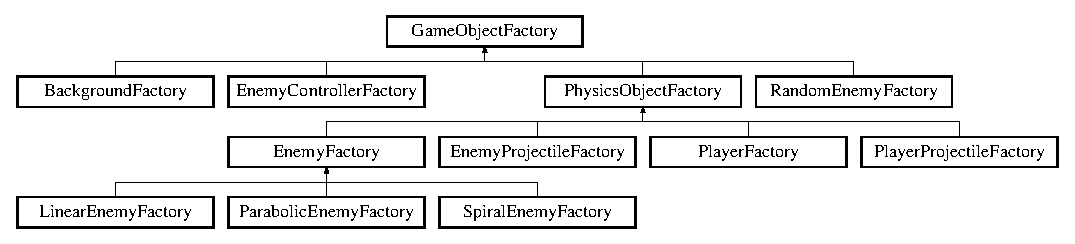
\includegraphics[height=2.835443cm]{d6/d7c/class_game_object_factory}
\end{center}
\end{figure}
\subsection*{Public Member Functions}
\begin{DoxyCompactItemize}
\item 
virtual std\+::shared\+\_\+ptr$<$ \hyperlink{class_game_object}{Game\+Object} $>$ \hyperlink{class_game_object_factory_a5b684a6e77fb82c041f1721eb07c553d}{get\+Game\+Object} (const std\+::shared\+\_\+ptr$<$ \hyperlink{class_database_interface}{Database\+Interface} $>$ \&database)
\begin{DoxyCompactList}\small\item\em virtual function used to create the desired class specified by the derived class \end{DoxyCompactList}\item 
virtual \hyperlink{struct_game_object_data}{Game\+Object\+Data} \hyperlink{class_game_object_factory_ae9358fbb3ef2d3b127320341760d3ff9}{get\+Object\+Data} (const std\+::shared\+\_\+ptr$<$ \hyperlink{class_database_interface}{Database\+Interface} $>$ \&database)=0
\begin{DoxyCompactList}\small\item\em used to obtain the specific \hyperlink{struct_game_object_data}{Game\+Object\+Data} defined for the current factory \end{DoxyCompactList}\end{DoxyCompactItemize}


\subsection{Detailed Description}
The interface class that is used to define the factory design pattern, it is used to create the various objects used within the game. 

\subsection{Member Function Documentation}
\mbox{\Hypertarget{class_game_object_factory_a5b684a6e77fb82c041f1721eb07c553d}\label{class_game_object_factory_a5b684a6e77fb82c041f1721eb07c553d}} 
\index{Game\+Object\+Factory@{Game\+Object\+Factory}!get\+Game\+Object@{get\+Game\+Object}}
\index{get\+Game\+Object@{get\+Game\+Object}!Game\+Object\+Factory@{Game\+Object\+Factory}}
\subsubsection{\texorpdfstring{get\+Game\+Object()}{getGameObject()}}
{\footnotesize\ttfamily std\+::shared\+\_\+ptr$<$ \hyperlink{class_game_object}{Game\+Object} $>$ Game\+Object\+Factory\+::get\+Game\+Object (\begin{DoxyParamCaption}\item[{const std\+::shared\+\_\+ptr$<$ \hyperlink{class_database_interface}{Database\+Interface} $>$ \&}]{database }\end{DoxyParamCaption})\hspace{0.3cm}{\ttfamily [virtual]}}



virtual function used to create the desired class specified by the derived class 

\begin{DoxyReturn}{Returns}
Returns the constructed \hyperlink{class_game_object}{Game\+Object} object 
\end{DoxyReturn}


Reimplemented in \hyperlink{class_background_factory_a17793b3ec704137388b70f53361691c3}{Background\+Factory}, \hyperlink{class_player_factory_ab92534e7d2d6887ecf9e4ed8131a8112}{Player\+Factory}, \hyperlink{class_enemy_factory_acb6ad18d5ef69a27927907fa9a444c7d}{Enemy\+Factory}, \hyperlink{class_random_enemy_factory_a5099fcf010a5cf2f53fd7c874a1925a9}{Random\+Enemy\+Factory}, \hyperlink{class_enemy_controller_factory_a6ab6c433cc498c7353a1ab2eb213664d}{Enemy\+Controller\+Factory}, \hyperlink{class_enemy_projectile_factory_a081c6bea7032956c278fdf4ff62d530a}{Enemy\+Projectile\+Factory}, \hyperlink{class_player_projectile_factory_a804a9f591ce6f0a7fb04f35ff685ff57}{Player\+Projectile\+Factory}, and \hyperlink{class_physics_object_factory_a2644107d0c455c3307559cd824a7c9a8}{Physics\+Object\+Factory}.

\mbox{\Hypertarget{class_game_object_factory_ae9358fbb3ef2d3b127320341760d3ff9}\label{class_game_object_factory_ae9358fbb3ef2d3b127320341760d3ff9}} 
\index{Game\+Object\+Factory@{Game\+Object\+Factory}!get\+Object\+Data@{get\+Object\+Data}}
\index{get\+Object\+Data@{get\+Object\+Data}!Game\+Object\+Factory@{Game\+Object\+Factory}}
\subsubsection{\texorpdfstring{get\+Object\+Data()}{getObjectData()}}
{\footnotesize\ttfamily virtual \hyperlink{struct_game_object_data}{Game\+Object\+Data} Game\+Object\+Factory\+::get\+Object\+Data (\begin{DoxyParamCaption}\item[{const std\+::shared\+\_\+ptr$<$ \hyperlink{class_database_interface}{Database\+Interface} $>$ \&}]{database }\end{DoxyParamCaption})\hspace{0.3cm}{\ttfamily [pure virtual]}}



used to obtain the specific \hyperlink{struct_game_object_data}{Game\+Object\+Data} defined for the current factory 


\begin{DoxyParams}{Parameters}
{\em database} & The specific \hyperlink{class_database_interface}{Database\+Interface} that contains the information about the Game\+Objects \\
\hline
\end{DoxyParams}
\begin{DoxyReturn}{Returns}
The \hyperlink{struct_game_object_data}{Game\+Object\+Data} required for the construction of the object 
\end{DoxyReturn}


Implemented in \hyperlink{class_background_factory_aed13815bcb56568c4b465b5a531ee053}{Background\+Factory}, \hyperlink{class_enemy_controller_factory_a27d4819c1174490c22f2e111f32ca2ec}{Enemy\+Controller\+Factory}, \hyperlink{class_enemy_projectile_factory_a1ef660e5962f29b7353054c6480477c7}{Enemy\+Projectile\+Factory}, \hyperlink{class_player_factory_aca4e809430541d77acd4c588c4381715}{Player\+Factory}, \hyperlink{class_random_enemy_factory_a7c007b44a5e5e59fecc0b8cd2a6a9dc3}{Random\+Enemy\+Factory}, \hyperlink{class_player_projectile_factory_a702ae964c9dc653140fad4e17f38f60a}{Player\+Projectile\+Factory}, \hyperlink{class_parabolic_enemy_factory_acc62c48a8eb5af162910dc48d9fe8900}{Parabolic\+Enemy\+Factory}, \hyperlink{class_physics_object_factory_aa59f52d3adc1fac676f4a8a3c2de9ba9}{Physics\+Object\+Factory}, \hyperlink{class_spiral_enemy_factory_a230709a0781c4364aa062b0bd441ec4d}{Spiral\+Enemy\+Factory}, and \hyperlink{class_linear_enemy_factory_a9d959b8a414e30ad4813d5d3740eafee}{Linear\+Enemy\+Factory}.



The documentation for this class was generated from the following files\+:\begin{DoxyCompactItemize}
\item 
C\+:/\+Users/\+Tim/\+Documents/\+Software\+Dev/\+Software\+Project/\+Project\+Files/game-\/source-\/code/\+Back\+End\+Systems/Game\+Object\+Factory.\+h\item 
C\+:/\+Users/\+Tim/\+Documents/\+Software\+Dev/\+Software\+Project/\+Project\+Files/game-\/source-\/code/\+Back\+End\+Systems/Game\+Object\+Factory.\+cpp\end{DoxyCompactItemize}

\hypertarget{class_game_object_type_construction_not_defined}{}\section{Game\+Object\+Type\+Construction\+Not\+Defined Class Reference}
\label{class_game_object_type_construction_not_defined}\index{Game\+Object\+Type\+Construction\+Not\+Defined@{Game\+Object\+Type\+Construction\+Not\+Defined}}


Exception thrown if a Game\+Object\+Type is consturcted during runtime and it has not been defined.  




{\ttfamily \#include $<$Repository.\+h$>$}



\subsection{Detailed Description}
Exception thrown if a Game\+Object\+Type is consturcted during runtime and it has not been defined. 

The documentation for this class was generated from the following file\+:\begin{DoxyCompactItemize}
\item 
C\+:/\+Users/\+Tim/\+Documents/\+Software\+Dev/\+Software\+Project/\+Project\+Files/game-\/source-\/code/\+Back\+End\+Systems/Repository.\+h\end{DoxyCompactItemize}

\hypertarget{class_game_scene_factory}{}\section{Game\+Scene\+Factory Class Reference}
\label{class_game_scene_factory}\index{Game\+Scene\+Factory@{Game\+Scene\+Factory}}


Constructs the \hyperlink{class_scene}{Scene} that is used for the main game.  




{\ttfamily \#include $<$Game\+Scene\+Factory.\+h$>$}

Inheritance diagram for Game\+Scene\+Factory\+:\begin{figure}[H]
\begin{center}
\leavevmode
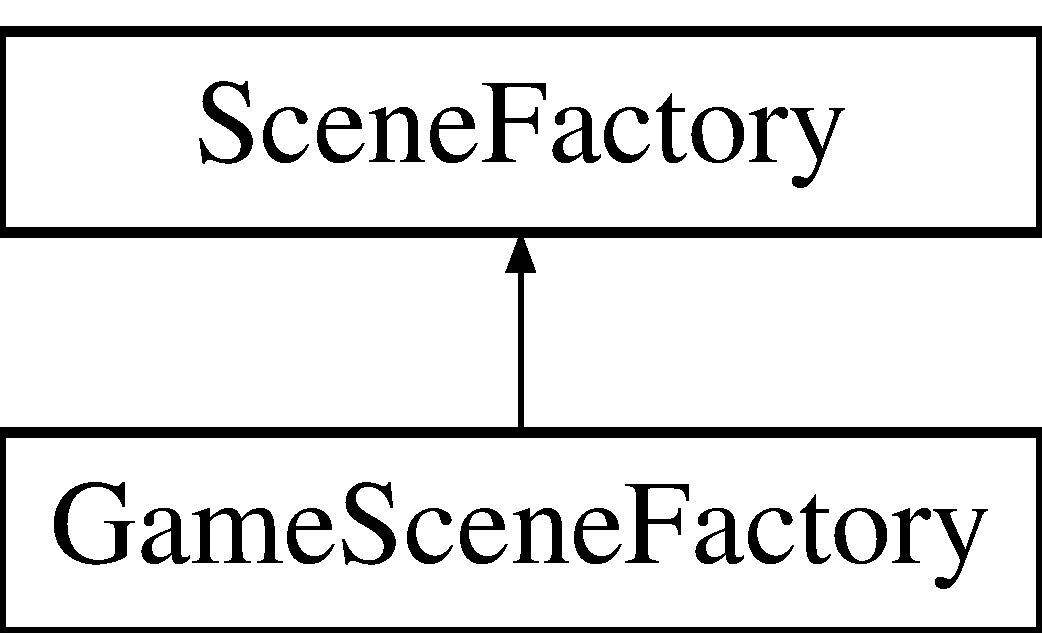
\includegraphics[height=2.000000cm]{da/da3/class_game_scene_factory}
\end{center}
\end{figure}
\subsection*{Protected Member Functions}
\begin{DoxyCompactItemize}
\item 
virtual std\+::list$<$ std\+::shared\+\_\+ptr$<$ \hyperlink{class_game_object}{Game\+Object} $>$ $>$ \hyperlink{class_game_scene_factory_a2db801c1a1703a14a00c7b6e8bdca5b0}{get\+Game\+Obect\+List} (std\+::shared\+\_\+ptr$<$ \hyperlink{class_database_interface}{Database\+Interface} $>$ database) const override
\begin{DoxyCompactList}\small\item\em Returns the game\+Object list required for the construction of the specific \hyperlink{class_scene}{Scene}. \end{DoxyCompactList}\end{DoxyCompactItemize}
\subsection*{Additional Inherited Members}


\subsection{Detailed Description}
Constructs the \hyperlink{class_scene}{Scene} that is used for the main game. 

\subsection{Member Function Documentation}
\mbox{\Hypertarget{class_game_scene_factory_a2db801c1a1703a14a00c7b6e8bdca5b0}\label{class_game_scene_factory_a2db801c1a1703a14a00c7b6e8bdca5b0}} 
\index{Game\+Scene\+Factory@{Game\+Scene\+Factory}!get\+Game\+Obect\+List@{get\+Game\+Obect\+List}}
\index{get\+Game\+Obect\+List@{get\+Game\+Obect\+List}!Game\+Scene\+Factory@{Game\+Scene\+Factory}}
\subsubsection{\texorpdfstring{get\+Game\+Obect\+List()}{getGameObectList()}}
{\footnotesize\ttfamily std\+::list$<$ std\+::shared\+\_\+ptr$<$ \hyperlink{class_game_object}{Game\+Object} $>$ $>$ Game\+Scene\+Factory\+::get\+Game\+Obect\+List (\begin{DoxyParamCaption}\item[{std\+::shared\+\_\+ptr$<$ \hyperlink{class_database_interface}{Database\+Interface} $>$}]{database }\end{DoxyParamCaption}) const\hspace{0.3cm}{\ttfamily [override]}, {\ttfamily [protected]}, {\ttfamily [virtual]}}



Returns the game\+Object list required for the construction of the specific \hyperlink{class_scene}{Scene}. 


\begin{DoxyParams}{Parameters}
{\em database} & The \hyperlink{class_database_interface}{Database\+Interface} that contains the information about the various Game\+Objects \\
\hline
\end{DoxyParams}


Implements \hyperlink{class_scene_factory_a2c8541230e95df49d2ab39b7c6ecdb78}{Scene\+Factory}.



The documentation for this class was generated from the following files\+:\begin{DoxyCompactItemize}
\item 
C\+:/\+Users/\+Tim/\+Documents/\+Software\+Dev/\+Software\+Project/\+Project\+Files/game-\/source-\/code/\+Back\+End\+Systems/Game\+Scene\+Factory.\+h\item 
C\+:/\+Users/\+Tim/\+Documents/\+Software\+Dev/\+Software\+Project/\+Project\+Files/game-\/source-\/code/\+Back\+End\+Systems/Game\+Scene\+Factory.\+cpp\end{DoxyCompactItemize}

\hypertarget{struct_game_state_data}{}\section{Game\+State\+Data Class Reference}
\label{struct_game_state_data}\index{Game\+State\+Data@{Game\+State\+Data}}


A struct used to contain all of the basic game information.  




{\ttfamily \#include $<$Game\+Data.\+h$>$}

\subsection*{Public Member Functions}
\begin{DoxyCompactItemize}
\item 
\mbox{\Hypertarget{struct_game_state_data_acb2da79775aed7c30863992956c1272e}\label{struct_game_state_data_acb2da79775aed7c30863992956c1272e}} 
{\bfseries Game\+State\+Data} (unsigned int scr\+\_\+sz\+\_\+x, unsigned int scr\+\_\+sz\+\_\+y, std\+::string game\+Name)
\item 
\mbox{\Hypertarget{struct_game_state_data_a1785e49ae998f451376aa910d5fe4ff1}\label{struct_game_state_data_a1785e49ae998f451376aa910d5fe4ff1}} 
bool {\bfseries operator==} (const \hyperlink{struct_game_state_data}{Game\+State\+Data} \&rhs) const
\end{DoxyCompactItemize}
\subsection*{Public Attributes}
\begin{DoxyCompactItemize}
\item 
\mbox{\Hypertarget{struct_game_state_data_a77ad6fb81bff60f557bca625796e7c4b}\label{struct_game_state_data_a77ad6fb81bff60f557bca625796e7c4b}} 
unsigned int {\bfseries screen\+\_\+size\+\_\+x} = 1920
\item 
\mbox{\Hypertarget{struct_game_state_data_a3e22c382b0b7a5cded66565b257e50e3}\label{struct_game_state_data_a3e22c382b0b7a5cded66565b257e50e3}} 
unsigned int {\bfseries screen\+\_\+size\+\_\+y} = 1080
\item 
\mbox{\Hypertarget{struct_game_state_data_a91d07a38bd67335ce65d01ec8f147411}\label{struct_game_state_data_a91d07a38bd67335ce65d01ec8f147411}} 
std\+::string {\bfseries game\+Name} = \char`\"{}Game\char`\"{}
\end{DoxyCompactItemize}


\subsection{Detailed Description}
A struct used to contain all of the basic game information. 

The documentation for this class was generated from the following files\+:\begin{DoxyCompactItemize}
\item 
D\+:/\+Users/\+Tim-\/\+P\+C/\+Documents/\+Software\+\_\+\+I\+I/\+Project/\+Project\+Files/game-\/source-\/code/\+Back\+End\+Systems/Game\+Data.\+h\item 
D\+:/\+Users/\+Tim-\/\+P\+C/\+Documents/\+Software\+\_\+\+I\+I/\+Project/\+Project\+Files/game-\/source-\/code/\+Back\+End\+Systems/Game\+Data.\+cpp\end{DoxyCompactItemize}

\hypertarget{class_game_time}{}\section{Game\+Time Class Reference}
\label{class_game_time}\index{Game\+Time@{Game\+Time}}


Determines the time that it takes for a single frame.  




{\ttfamily \#include $<$Game\+Time.\+h$>$}

\subsection*{Public Member Functions}
\begin{DoxyCompactItemize}
\item 
\mbox{\Hypertarget{class_game_time_ab3b7fbfbc2a94e223d349b3dd48f76d3}\label{class_game_time_ab3b7fbfbc2a94e223d349b3dd48f76d3}} 
\hyperlink{class_game_time_ab3b7fbfbc2a94e223d349b3dd48f76d3}{Game\+Time} ()
\begin{DoxyCompactList}\small\item\em Constructs the \hyperlink{class_game_time}{Game\+Time} object and seeds the random generator. \end{DoxyCompactList}\item 
\mbox{\Hypertarget{class_game_time_a424d4e2f4745a85897620751ff5153b9}\label{class_game_time_a424d4e2f4745a85897620751ff5153b9}} 
void \hyperlink{class_game_time_a424d4e2f4745a85897620751ff5153b9}{Time\+Frame} ()
\begin{DoxyCompactList}\small\item\em Times the current frame and determines the new delta time. \end{DoxyCompactList}\end{DoxyCompactItemize}
\subsection*{Static Public Member Functions}
\begin{DoxyCompactItemize}
\item 
static double \hyperlink{class_game_time_aa5ea84c887116ef68d1331617c5a81c3}{get\+Delta\+Time} ()
\begin{DoxyCompactList}\small\item\em Returns the difference in time between the last frame and the current frame. \end{DoxyCompactList}\end{DoxyCompactItemize}
\subsection*{Private Member Functions}
\begin{DoxyCompactItemize}
\item 
double \hyperlink{class_game_time_ac8a380f740f5bc39e98fda3e069c0bb3}{calc\+Process\+Time} ()
\begin{DoxyCompactList}\small\item\em Determines the amount of time that has passes since the game began running, converts it into a double and returns the value. \end{DoxyCompactList}\item 
\mbox{\Hypertarget{class_game_time_a8575cb09f1e07b90678eedaf92776a97}\label{class_game_time_a8575cb09f1e07b90678eedaf92776a97}} 
void \hyperlink{class_game_time_a8575cb09f1e07b90678eedaf92776a97}{calc\+Delta\+Time} ()
\begin{DoxyCompactList}\small\item\em Calculates the time between the current frame and the last frame. \end{DoxyCompactList}\item 
\mbox{\Hypertarget{class_game_time_aec3fa5e495f783524701418f5d679071}\label{class_game_time_aec3fa5e495f783524701418f5d679071}} 
void \hyperlink{class_game_time_aec3fa5e495f783524701418f5d679071}{calc\+Current\+Time} ()
\begin{DoxyCompactList}\small\item\em Calculates the time up until the current frame. \end{DoxyCompactList}\end{DoxyCompactItemize}
\subsection*{Static Private Attributes}
\begin{DoxyCompactItemize}
\item 
static double \hyperlink{class_game_time_a080d9deb72c675f0d68f9ad72eec66c3}{\+\_\+current\+\_\+time} = 0
\begin{DoxyCompactList}\small\item\em variables and names need to be changed to make it more understandable \end{DoxyCompactList}\item 
static double \hyperlink{class_game_time_a39c7a52db277a99fd6dfcb457b432d7d}{\+\_\+delta\+Time} = 1
\end{DoxyCompactItemize}


\subsection{Detailed Description}
Determines the time that it takes for a single frame. 

Used to create smooth interactions between the Game logic and the Back\+End\+Systems 

\subsection{Member Function Documentation}
\mbox{\Hypertarget{class_game_time_ac8a380f740f5bc39e98fda3e069c0bb3}\label{class_game_time_ac8a380f740f5bc39e98fda3e069c0bb3}} 
\index{Game\+Time@{Game\+Time}!calc\+Process\+Time@{calc\+Process\+Time}}
\index{calc\+Process\+Time@{calc\+Process\+Time}!Game\+Time@{Game\+Time}}
\subsubsection{\texorpdfstring{calc\+Process\+Time()}{calcProcessTime()}}
{\footnotesize\ttfamily double Game\+Time\+::calc\+Process\+Time (\begin{DoxyParamCaption}{ }\end{DoxyParamCaption})\hspace{0.3cm}{\ttfamily [private]}}



Determines the amount of time that has passes since the game began running, converts it into a double and returns the value. 

\begin{DoxyReturn}{Returns}
Returns the amount of time that has passed since the game began 
\end{DoxyReturn}
\mbox{\Hypertarget{class_game_time_aa5ea84c887116ef68d1331617c5a81c3}\label{class_game_time_aa5ea84c887116ef68d1331617c5a81c3}} 
\index{Game\+Time@{Game\+Time}!get\+Delta\+Time@{get\+Delta\+Time}}
\index{get\+Delta\+Time@{get\+Delta\+Time}!Game\+Time@{Game\+Time}}
\subsubsection{\texorpdfstring{get\+Delta\+Time()}{getDeltaTime()}}
{\footnotesize\ttfamily double Game\+Time\+::get\+Delta\+Time (\begin{DoxyParamCaption}{ }\end{DoxyParamCaption})\hspace{0.3cm}{\ttfamily [static]}}



Returns the difference in time between the last frame and the current frame. 

\begin{DoxyReturn}{Returns}
Returns the difference in time between the last frame and the current frame 
\end{DoxyReturn}


\subsection{Member Data Documentation}
\mbox{\Hypertarget{class_game_time_a080d9deb72c675f0d68f9ad72eec66c3}\label{class_game_time_a080d9deb72c675f0d68f9ad72eec66c3}} 
\index{Game\+Time@{Game\+Time}!\+\_\+current\+\_\+time@{\+\_\+current\+\_\+time}}
\index{\+\_\+current\+\_\+time@{\+\_\+current\+\_\+time}!Game\+Time@{Game\+Time}}
\subsubsection{\texorpdfstring{\+\_\+current\+\_\+time}{\_current\_time}}
{\footnotesize\ttfamily double Game\+Time\+::\+\_\+current\+\_\+time = 0\hspace{0.3cm}{\ttfamily [static]}, {\ttfamily [private]}}



variables and names need to be changed to make it more understandable 

current time up till the current frame \mbox{\Hypertarget{class_game_time_a39c7a52db277a99fd6dfcb457b432d7d}\label{class_game_time_a39c7a52db277a99fd6dfcb457b432d7d}} 
\index{Game\+Time@{Game\+Time}!\+\_\+delta\+Time@{\+\_\+delta\+Time}}
\index{\+\_\+delta\+Time@{\+\_\+delta\+Time}!Game\+Time@{Game\+Time}}
\subsubsection{\texorpdfstring{\+\_\+delta\+Time}{\_deltaTime}}
{\footnotesize\ttfamily double Game\+Time\+::\+\_\+delta\+Time = 1\hspace{0.3cm}{\ttfamily [static]}, {\ttfamily [private]}}

change in time between frames 

The documentation for this class was generated from the following files\+:\begin{DoxyCompactItemize}
\item 
D\+:/\+Users/\+Tim-\/\+P\+C/\+Documents/\+Software\+\_\+\+I\+I/\+Project/\+Project\+Files/game-\/source-\/code/\+Back\+End\+Systems/Game\+Time.\+h\item 
D\+:/\+Users/\+Tim-\/\+P\+C/\+Documents/\+Software\+\_\+\+I\+I/\+Project/\+Project\+Files/game-\/source-\/code/\+Back\+End\+Systems/Game\+Time.\+cpp\end{DoxyCompactItemize}

\hypertarget{class_graphic_name_reservedfor_null_graphic}{}\section{Graphic\+Name\+Reservedfor\+Null\+Graphic Class Reference}
\label{class_graphic_name_reservedfor_null_graphic}\index{Graphic\+Name\+Reservedfor\+Null\+Graphic@{Graphic\+Name\+Reservedfor\+Null\+Graphic}}


The documentation for this class was generated from the following file\+:\begin{DoxyCompactItemize}
\item 
D\+:/\+Users/\+Tim-\/\+P\+C/\+Documents/\+Software\+\_\+\+I\+I/\+Project/\+Project\+Files/game-\/source-\/code/\+Front\+End\+Systems/Graphic\+Object.\+cpp\end{DoxyCompactItemize}

\hypertarget{class_graphic_object}{}\section{Graphic\+Object Class Reference}
\label{class_graphic_object}\index{Graphic\+Object@{Graphic\+Object}}


This is the Utility class with the display manager, It stores the name of the object and location of the image file which are both necessary for the \hyperlink{class_display_manager}{Display\+Manager} to correctly display the specified image.  




{\ttfamily \#include $<$Graphic\+Object.\+h$>$}

\subsection*{Public Member Functions}
\begin{DoxyCompactItemize}
\item 
\mbox{\Hypertarget{class_graphic_object_ae1b56ae4484ad120f5ba77c0b683a045}\label{class_graphic_object_ae1b56ae4484ad120f5ba77c0b683a045}} 
\hyperlink{class_graphic_object_ae1b56ae4484ad120f5ba77c0b683a045}{Graphic\+Object} ()
\begin{DoxyCompactList}\small\item\em Default Constructor, creates a Null\+Graphic by default. \end{DoxyCompactList}\item 
\mbox{\Hypertarget{class_graphic_object_a4a14ca7f3b9e9736b0b4231ee08dc0ab}\label{class_graphic_object_a4a14ca7f3b9e9736b0b4231ee08dc0ab}} 
\hyperlink{class_graphic_object_a4a14ca7f3b9e9736b0b4231ee08dc0ab}{Graphic\+Object} (const \hyperlink{class_graphic_object}{Graphic\+Object} \&copy)
\begin{DoxyCompactList}\small\item\em Copy Constructor of \hyperlink{class_graphic_object}{Graphic\+Object}. \end{DoxyCompactList}\item 
\mbox{\Hypertarget{class_graphic_object_a4026dc4e922a5053b6c0e3d1a9b28b63}\label{class_graphic_object_a4026dc4e922a5053b6c0e3d1a9b28b63}} 
\hyperlink{class_graphic_object}{Graphic\+Object} \& \hyperlink{class_graphic_object_a4026dc4e922a5053b6c0e3d1a9b28b63}{operator=} (const \hyperlink{class_graphic_object}{Graphic\+Object} \&rhs)
\begin{DoxyCompactList}\small\item\em Assignment operator overload. \end{DoxyCompactList}\item 
\hyperlink{class_graphic_object_a9819ca0b4c1bb72ede070d8485bfc8a9}{Graphic\+Object} (string texture\+Location, string graphic\+Name)
\begin{DoxyCompactList}\small\item\em Standard Constructor, creates a Graphic Object with the client specified parameters. \end{DoxyCompactList}\item 
const string \& \hyperlink{class_graphic_object_a8772813296b837e997ee21836e92b028}{get\+Graphic\+Name} () const
\begin{DoxyCompactList}\small\item\em Getter is necessary to decouple the presentation layer from the game logic layer. \end{DoxyCompactList}\item 
const string \& \hyperlink{class_graphic_object_a1041a2dd82f82fc724675c5a2ea67d32}{get\+Texture\+Location} () const
\begin{DoxyCompactList}\small\item\em Getter is necessary to decouple the presentation layer from the game logic layer. \end{DoxyCompactList}\end{DoxyCompactItemize}
\subsection*{Static Public Attributes}
\begin{DoxyCompactItemize}
\item 
\mbox{\Hypertarget{class_graphic_object_a3a6832e8f4af96da2935d3c69757107c}\label{class_graphic_object_a3a6832e8f4af96da2935d3c69757107c}} 
static const \hyperlink{class_graphic_object}{Graphic\+Object} \hyperlink{class_graphic_object_a3a6832e8f4af96da2935d3c69757107c}{Null\+Graphic} \{\char`\"{}Null\char`\"{}, \char`\"{}Null\+Graphic.\+png\char`\"{}\}
\begin{DoxyCompactList}\small\item\em Null\+Graphic Declaration, requires the \char`\"{}\+Null\+Graphic.\+png\char`\"{} image to be available. \end{DoxyCompactList}\end{DoxyCompactItemize}
\subsection*{Protected Attributes}
\begin{DoxyCompactItemize}
\item 
std\+::string \hyperlink{class_graphic_object_a3fc571887a6e46dda4a4ef10d44720b5}{\+\_\+texture\+Location}
\item 
std\+::string \hyperlink{class_graphic_object_a74c9292d37d9be9e099c868be084b33f}{\+\_\+graphic\+Name}
\end{DoxyCompactItemize}


\subsection{Detailed Description}
This is the Utility class with the display manager, It stores the name of the object and location of the image file which are both necessary for the \hyperlink{class_display_manager}{Display\+Manager} to correctly display the specified image. 

The Graphic Object has a tight coupling with the Presentation layer classes. The graphic name of the object is used as a key within a hashtable to identify the specific sfml sprite and texture that needs to be drawn for the corresponding object. \hyperlink{class_graphic_object}{Graphic\+Object} acts as a link between the Presentation Layer and the Domain layer. It forms a composition relationship with the \hyperlink{class_game_object}{Game\+Object} class. A Null\+Object is assigned by default for derived implimentations of \hyperlink{class_game_object}{Game\+Object} that do not require a \hyperlink{class_graphic_object}{Graphic\+Object} The Null\+Object consistis of a Null\+Object.\+png image which is a single transparent pixel and the graphic\+Name Null. This is an Object name that is preserved by the constructor. ie another \hyperlink{class_graphic_object}{Graphic\+Object} may not have the name Null. 

\subsection{Constructor \& Destructor Documentation}
\mbox{\Hypertarget{class_graphic_object_a9819ca0b4c1bb72ede070d8485bfc8a9}\label{class_graphic_object_a9819ca0b4c1bb72ede070d8485bfc8a9}} 
\index{Graphic\+Object@{Graphic\+Object}!Graphic\+Object@{Graphic\+Object}}
\index{Graphic\+Object@{Graphic\+Object}!Graphic\+Object@{Graphic\+Object}}
\subsubsection{\texorpdfstring{Graphic\+Object()}{GraphicObject()}}
{\footnotesize\ttfamily Graphic\+Object\+::\+Graphic\+Object (\begin{DoxyParamCaption}\item[{string}]{texture\+Location,  }\item[{string}]{graphic\+Name }\end{DoxyParamCaption})}



Standard Constructor, creates a Graphic Object with the client specified parameters. 


\begin{DoxyParams}{Parameters}
{\em texture\+Location} & The texture location for the image that the object uses \\
\hline
{\em graphic\+Name} & The name of that corresponds to objects that use the same image\\
\hline
\end{DoxyParams}
Checks if the reserved graphic\+Name \char`\"{}\+Null\char`\"{} is used, throws \hyperlink{class_graphic_name_reservedfor_null_graphic}{Graphic\+Name\+Reservedfor\+Null\+Graphic} if Null is used 

\subsection{Member Function Documentation}
\mbox{\Hypertarget{class_graphic_object_a8772813296b837e997ee21836e92b028}\label{class_graphic_object_a8772813296b837e997ee21836e92b028}} 
\index{Graphic\+Object@{Graphic\+Object}!get\+Graphic\+Name@{get\+Graphic\+Name}}
\index{get\+Graphic\+Name@{get\+Graphic\+Name}!Graphic\+Object@{Graphic\+Object}}
\subsubsection{\texorpdfstring{get\+Graphic\+Name()}{getGraphicName()}}
{\footnotesize\ttfamily const string\& Graphic\+Object\+::get\+Graphic\+Name (\begin{DoxyParamCaption}{ }\end{DoxyParamCaption}) const\hspace{0.3cm}{\ttfamily [inline]}}



Getter is necessary to decouple the presentation layer from the game logic layer. 

\begin{DoxyReturn}{Returns}
Returns a constant string that represents the graphic name of the object 
\end{DoxyReturn}
\mbox{\Hypertarget{class_graphic_object_a1041a2dd82f82fc724675c5a2ea67d32}\label{class_graphic_object_a1041a2dd82f82fc724675c5a2ea67d32}} 
\index{Graphic\+Object@{Graphic\+Object}!get\+Texture\+Location@{get\+Texture\+Location}}
\index{get\+Texture\+Location@{get\+Texture\+Location}!Graphic\+Object@{Graphic\+Object}}
\subsubsection{\texorpdfstring{get\+Texture\+Location()}{getTextureLocation()}}
{\footnotesize\ttfamily const string\& Graphic\+Object\+::get\+Texture\+Location (\begin{DoxyParamCaption}{ }\end{DoxyParamCaption}) const\hspace{0.3cm}{\ttfamily [inline]}}



Getter is necessary to decouple the presentation layer from the game logic layer. 

\begin{DoxyReturn}{Returns}
Returns a constant string that represents the location of the image file that is being used 
\end{DoxyReturn}


\subsection{Member Data Documentation}
\mbox{\Hypertarget{class_graphic_object_a74c9292d37d9be9e099c868be084b33f}\label{class_graphic_object_a74c9292d37d9be9e099c868be084b33f}} 
\index{Graphic\+Object@{Graphic\+Object}!\+\_\+graphic\+Name@{\+\_\+graphic\+Name}}
\index{\+\_\+graphic\+Name@{\+\_\+graphic\+Name}!Graphic\+Object@{Graphic\+Object}}
\subsubsection{\texorpdfstring{\+\_\+graphic\+Name}{\_graphicName}}
{\footnotesize\ttfamily std\+::string Graphic\+Object\+::\+\_\+graphic\+Name\hspace{0.3cm}{\ttfamily [protected]}}

The name used to load objects specified by the texture location$>$ \mbox{\Hypertarget{class_graphic_object_a3fc571887a6e46dda4a4ef10d44720b5}\label{class_graphic_object_a3fc571887a6e46dda4a4ef10d44720b5}} 
\index{Graphic\+Object@{Graphic\+Object}!\+\_\+texture\+Location@{\+\_\+texture\+Location}}
\index{\+\_\+texture\+Location@{\+\_\+texture\+Location}!Graphic\+Object@{Graphic\+Object}}
\subsubsection{\texorpdfstring{\+\_\+texture\+Location}{\_textureLocation}}
{\footnotesize\ttfamily std\+::string Graphic\+Object\+::\+\_\+texture\+Location\hspace{0.3cm}{\ttfamily [protected]}}

The location of the Image that the object represents$>$ 

The documentation for this class was generated from the following files\+:\begin{DoxyCompactItemize}
\item 
D\+:/\+Users/\+Tim-\/\+P\+C/\+Documents/\+Software\+\_\+\+I\+I/\+Project/\+Project\+Files/game-\/source-\/code/\+Front\+End\+Systems/Graphic\+Object.\+h\item 
D\+:/\+Users/\+Tim-\/\+P\+C/\+Documents/\+Software\+\_\+\+I\+I/\+Project/\+Project\+Files/game-\/source-\/code/\+Front\+End\+Systems/Graphic\+Object.\+cpp\end{DoxyCompactItemize}

\hypertarget{class_input}{}\section{Input Class Reference}
\label{class_input}\index{Input@{Input}}


Responsible for supplying the Front\+End\+System with access to the input of the user by interfaceing with sfml.  




{\ttfamily \#include $<$Input.\+h$>$}

\subsection*{Static Public Member Functions}
\begin{DoxyCompactItemize}
\item 
static bool \hyperlink{class_input_abb8551549ffe7b1474aca91ce3509d57}{Is\+Button\+Pressed} (Keys key)
\begin{DoxyCompactList}\small\item\em returns a boolean for the specific key that is pressed , returns true if the Key has been pressed \end{DoxyCompactList}\item 
static int \hyperlink{class_input_a5c4b1c67c7d3e28d4af79601c81ed8bb}{get\+Axis} (Axis axis)
\begin{DoxyCompactList}\small\item\em Provides directional information inherintly,. \end{DoxyCompactList}\item 
static void \hyperlink{class_input_a851f7b43b30dcf7166af7c548d21316f}{set\+Button} (Keys key, bool state)
\begin{DoxyCompactList}\small\item\em Sets the specific Key to the desired state of whether it is pressed or not. \end{DoxyCompactList}\end{DoxyCompactItemize}
\subsection*{Static Private Member Functions}
\begin{DoxyCompactItemize}
\item 
static int \hyperlink{class_input_a7419956b2d6001cef104b8abdf242477}{Check\+Button\+For\+Axis} (Keys negative\+Key, Keys positive\+Key)
\end{DoxyCompactItemize}
\subsection*{Static Private Attributes}
\begin{DoxyCompactItemize}
\item 
static std\+::vector$<$ bool $>$ \hyperlink{class_input_affef708e1d603d97a7218b64eab063b5}{\+\_\+buttons}
\end{DoxyCompactItemize}


\subsection{Detailed Description}
Responsible for supplying the Front\+End\+System with access to the input of the user by interfaceing with sfml. 

\subsection{Member Function Documentation}
\mbox{\Hypertarget{class_input_a7419956b2d6001cef104b8abdf242477}\label{class_input_a7419956b2d6001cef104b8abdf242477}} 
\index{Input@{Input}!Check\+Button\+For\+Axis@{Check\+Button\+For\+Axis}}
\index{Check\+Button\+For\+Axis@{Check\+Button\+For\+Axis}!Input@{Input}}
\subsubsection{\texorpdfstring{Check\+Button\+For\+Axis()}{CheckButtonForAxis()}}
{\footnotesize\ttfamily int Input\+::\+Check\+Button\+For\+Axis (\begin{DoxyParamCaption}\item[{Keys}]{negative\+Key,  }\item[{Keys}]{positive\+Key }\end{DoxyParamCaption})\hspace{0.3cm}{\ttfamily [static]}, {\ttfamily [private]}}

Uses the buttons to determine direction from button presses \mbox{\Hypertarget{class_input_a5c4b1c67c7d3e28d4af79601c81ed8bb}\label{class_input_a5c4b1c67c7d3e28d4af79601c81ed8bb}} 
\index{Input@{Input}!get\+Axis@{get\+Axis}}
\index{get\+Axis@{get\+Axis}!Input@{Input}}
\subsubsection{\texorpdfstring{get\+Axis()}{getAxis()}}
{\footnotesize\ttfamily int Input\+::get\+Axis (\begin{DoxyParamCaption}\item[{Axis}]{axis }\end{DoxyParamCaption})\hspace{0.3cm}{\ttfamily [static]}}



Provides directional information inherintly,. 


\begin{DoxyParams}{Parameters}
{\em axis} & The axis that the input occurs on \\
\hline
\end{DoxyParams}
\begin{DoxyReturn}{Returns}
Returns a -\/1, 0, or 1 depending on the direction and axis that was pressed 
\end{DoxyReturn}
\mbox{\Hypertarget{class_input_abb8551549ffe7b1474aca91ce3509d57}\label{class_input_abb8551549ffe7b1474aca91ce3509d57}} 
\index{Input@{Input}!Is\+Button\+Pressed@{Is\+Button\+Pressed}}
\index{Is\+Button\+Pressed@{Is\+Button\+Pressed}!Input@{Input}}
\subsubsection{\texorpdfstring{Is\+Button\+Pressed()}{IsButtonPressed()}}
{\footnotesize\ttfamily bool Input\+::\+Is\+Button\+Pressed (\begin{DoxyParamCaption}\item[{Keys}]{key }\end{DoxyParamCaption})\hspace{0.3cm}{\ttfamily [static]}}



returns a boolean for the specific key that is pressed , returns true if the Key has been pressed 


\begin{DoxyParams}{Parameters}
{\em key} & The specific key that needs to be checked if an input is detected \\
\hline
\end{DoxyParams}
\begin{DoxyReturn}{Returns}

\end{DoxyReturn}
\mbox{\Hypertarget{class_input_a851f7b43b30dcf7166af7c548d21316f}\label{class_input_a851f7b43b30dcf7166af7c548d21316f}} 
\index{Input@{Input}!set\+Button@{set\+Button}}
\index{set\+Button@{set\+Button}!Input@{Input}}
\subsubsection{\texorpdfstring{set\+Button()}{setButton()}}
{\footnotesize\ttfamily void Input\+::set\+Button (\begin{DoxyParamCaption}\item[{Keys}]{key,  }\item[{bool}]{state }\end{DoxyParamCaption})\hspace{0.3cm}{\ttfamily [static]}}



Sets the specific Key to the desired state of whether it is pressed or not. 


\begin{DoxyParams}{Parameters}
{\em key} & the specific key that is pressed or released \\
\hline
{\em state} & the desired state \\
\hline
\end{DoxyParams}


\subsection{Member Data Documentation}
\mbox{\Hypertarget{class_input_affef708e1d603d97a7218b64eab063b5}\label{class_input_affef708e1d603d97a7218b64eab063b5}} 
\index{Input@{Input}!\+\_\+buttons@{\+\_\+buttons}}
\index{\+\_\+buttons@{\+\_\+buttons}!Input@{Input}}
\subsubsection{\texorpdfstring{\+\_\+buttons}{\_buttons}}
{\footnotesize\ttfamily std\+::vector$<$ bool $>$ Input\+::\+\_\+buttons\hspace{0.3cm}{\ttfamily [static]}, {\ttfamily [private]}}

a vector of bools that are indexed by the enumerator 

The documentation for this class was generated from the following files\+:\begin{DoxyCompactItemize}
\item 
C\+:/\+Users/\+Tim/\+Documents/\+Software\+Dev/\+Software\+Project/\+Project\+Files/game-\/source-\/code/\+Back\+End\+Systems/Input.\+h\item 
C\+:/\+Users/\+Tim/\+Documents/\+Software\+Dev/\+Software\+Project/\+Project\+Files/game-\/source-\/code/\+Back\+End\+Systems/Input.\+cpp\end{DoxyCompactItemize}

\hypertarget{class_laser_generator_container}{}\section{Laser\+Generator\+Container Class Reference}
\label{class_laser_generator_container}\index{Laser\+Generator\+Container@{Laser\+Generator\+Container}}
Inheritance diagram for Laser\+Generator\+Container\+:\begin{figure}[H]
\begin{center}
\leavevmode
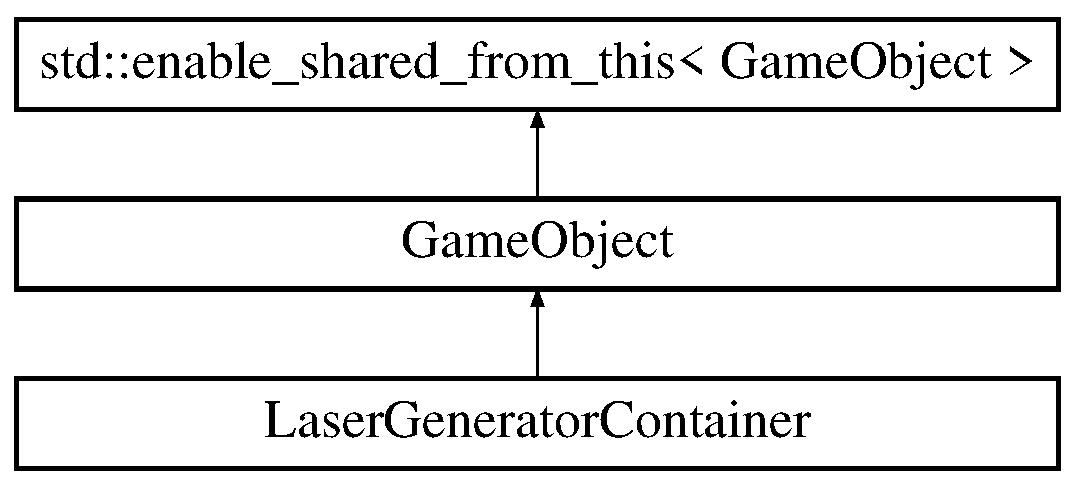
\includegraphics[height=3.000000cm]{dd/d9a/class_laser_generator_container}
\end{center}
\end{figure}
\subsection*{Public Member Functions}
\begin{DoxyCompactItemize}
\item 
\mbox{\Hypertarget{class_laser_generator_container_a682432fe75fbca52e43c5fef2e3473ae}\label{class_laser_generator_container_a682432fe75fbca52e43c5fef2e3473ae}} 
{\bfseries Laser\+Generator\+Container} (Laser\+Generator generator1, Laser\+Generator generator2, std\+::vector$<$ std\+::shared\+\_\+ptr$<$ \hyperlink{class_game_object}{Game\+Object} $>$$>$ laser\+Objects)
\item 
void \hyperlink{class_laser_generator_container_a9fc676b255f742a97ec0eb6036491684}{Start} ()
\begin{DoxyCompactList}\small\item\em Used for initialisation of the objects parameters when it is instantiated. \end{DoxyCompactList}\item 
\mbox{\Hypertarget{class_laser_generator_container_abd2fe127203087ed4642101e1f738b05}\label{class_laser_generator_container_abd2fe127203087ed4642101e1f738b05}} 
void {\bfseries Laser\+Generator\+Destroyed} ()
\end{DoxyCompactItemize}
\subsection*{Private Attributes}
\begin{DoxyCompactItemize}
\item 
\mbox{\Hypertarget{class_laser_generator_container_adf4406a310a5c67eabace28f364e008c}\label{class_laser_generator_container_adf4406a310a5c67eabace28f364e008c}} 
std\+::vector$<$ std\+::shared\+\_\+ptr$<$ \hyperlink{class_game_object}{Game\+Object} $>$ $>$ {\bfseries \+\_\+laser\+Objects}
\item 
\mbox{\Hypertarget{class_laser_generator_container_a8c690ffb366df925a29926b7988399d3}\label{class_laser_generator_container_a8c690ffb366df925a29926b7988399d3}} 
std\+::shared\+\_\+ptr$<$ Laser\+Generator $>$ {\bfseries \+\_\+laser\+Generator1}
\item 
\mbox{\Hypertarget{class_laser_generator_container_abdc918ac8e5ebba549e131145ad6d954}\label{class_laser_generator_container_abdc918ac8e5ebba549e131145ad6d954}} 
std\+::shared\+\_\+ptr$<$ Laser\+Generator $>$ {\bfseries \+\_\+laser\+Generator2}
\item 
\mbox{\Hypertarget{class_laser_generator_container_a36689e4d1a876aff7fb27a4fdc07c134}\label{class_laser_generator_container_a36689e4d1a876aff7fb27a4fdc07c134}} 
unsigned int {\bfseries \+\_\+number\+Of\+Generators\+Destroyed} = 0
\end{DoxyCompactItemize}
\subsection*{Additional Inherited Members}


\subsection{Member Function Documentation}
\mbox{\Hypertarget{class_laser_generator_container_a9fc676b255f742a97ec0eb6036491684}\label{class_laser_generator_container_a9fc676b255f742a97ec0eb6036491684}} 
\index{Laser\+Generator\+Container@{Laser\+Generator\+Container}!Start@{Start}}
\index{Start@{Start}!Laser\+Generator\+Container@{Laser\+Generator\+Container}}
\subsubsection{\texorpdfstring{Start()}{Start()}}
{\footnotesize\ttfamily void Laser\+Generator\+Container\+::\+Start (\begin{DoxyParamCaption}{ }\end{DoxyParamCaption})\hspace{0.3cm}{\ttfamily [inline]}, {\ttfamily [virtual]}}



Used for initialisation of the objects parameters when it is instantiated. 

Start is used to define the various intitialisation parameters that an object may require to be set before it exists inside of the game scene. The \hyperlink{class_scene}{Scene} Object calls this function when it is instantiated 

Reimplemented from \hyperlink{class_game_object_aeeb2162f2779e5591a372a1568bc5c68}{Game\+Object}.



The documentation for this class was generated from the following file\+:\begin{DoxyCompactItemize}
\item 
C\+:/\+Users/\+Tim/\+Documents/\+Software\+Dev/\+Software\+Project/\+Project\+Files/game-\/source-\/code/\+Front\+End\+Systems/Laser\+Generator.\+h\end{DoxyCompactItemize}

\hypertarget{class_linear_enemy_factory}{}\section{Linear\+Enemy\+Factory Class Reference}
\label{class_linear_enemy_factory}\index{Linear\+Enemy\+Factory@{Linear\+Enemy\+Factory}}


Constructs an \hyperlink{class_enemy}{Enemy} that moves in a straight line from the origin outwards.  




{\ttfamily \#include $<$Linear\+Enemy\+Factory.\+h$>$}

Inheritance diagram for Linear\+Enemy\+Factory\+:\begin{figure}[H]
\begin{center}
\leavevmode
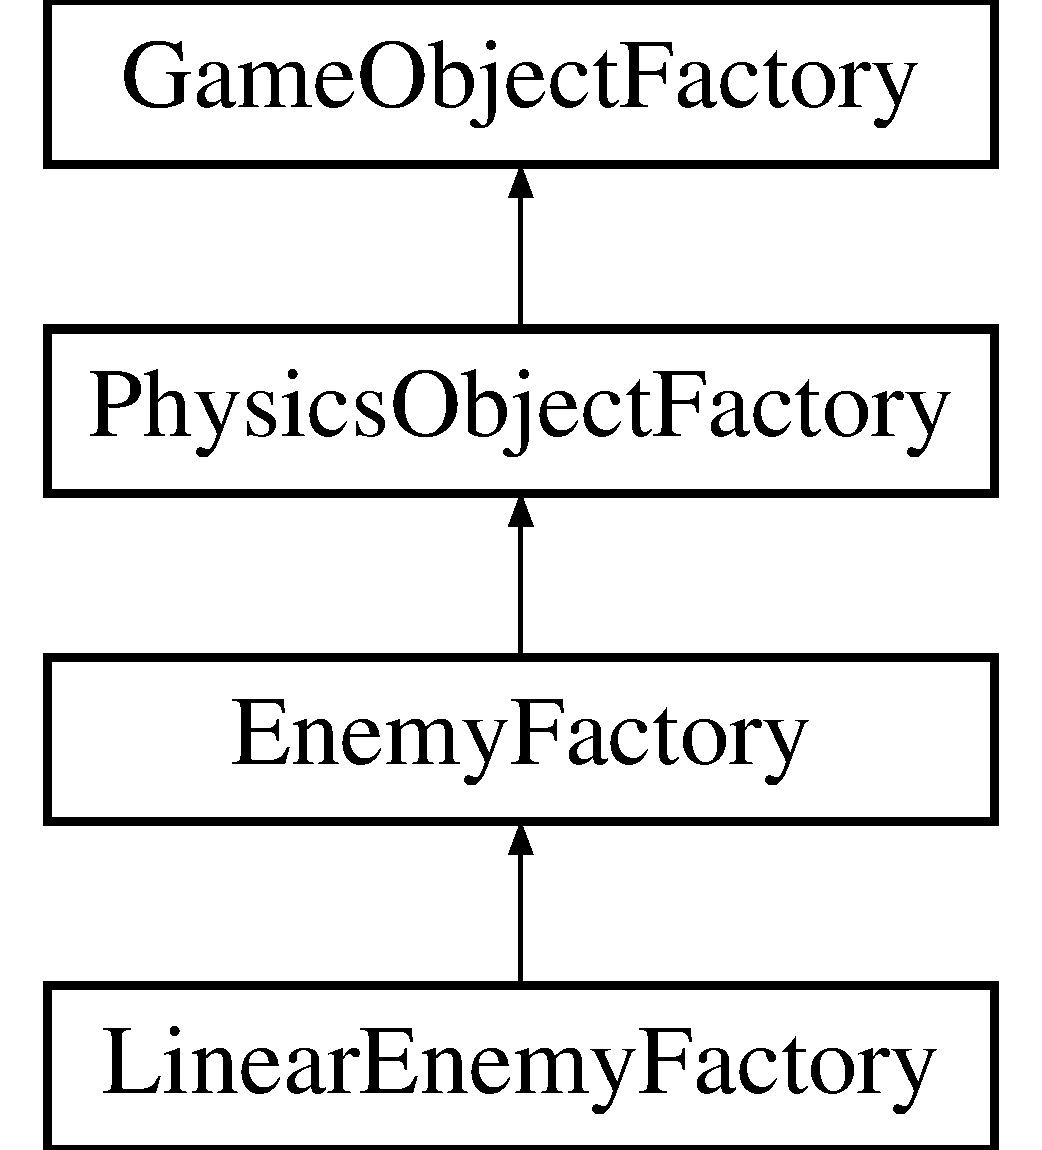
\includegraphics[height=4.000000cm]{d4/d4f/class_linear_enemy_factory}
\end{center}
\end{figure}
\subsection*{Public Member Functions}
\begin{DoxyCompactItemize}
\item 
virtual std\+::shared\+\_\+ptr$<$ \hyperlink{class_movable_interface}{Movable\+Interface} $>$ \hyperlink{class_linear_enemy_factory_ad8b2931b7f31f9f8e13d3c9d804469bf}{get\+Movable\+Type} (const \hyperlink{struct_game_object_data}{Game\+Object\+Data} \&data) override
\begin{DoxyCompactList}\small\item\em Pure virtual function used to assign the various Movable\+Interfaces that the Enemy\+Objects use. \end{DoxyCompactList}\item 
virtual \hyperlink{struct_game_object_data}{Game\+Object\+Data} \hyperlink{class_linear_enemy_factory_a9d959b8a414e30ad4813d5d3740eafee}{get\+Object\+Data} (const std\+::shared\+\_\+ptr$<$ \hyperlink{class_database_interface}{Database\+Interface} $>$ \&database) override
\begin{DoxyCompactList}\small\item\em used to obtain the specific \hyperlink{struct_game_object_data}{Game\+Object\+Data} defined for the current factory \end{DoxyCompactList}\end{DoxyCompactItemize}


\subsection{Detailed Description}
Constructs an \hyperlink{class_enemy}{Enemy} that moves in a straight line from the origin outwards. 

\subsection{Member Function Documentation}
\mbox{\Hypertarget{class_linear_enemy_factory_ad8b2931b7f31f9f8e13d3c9d804469bf}\label{class_linear_enemy_factory_ad8b2931b7f31f9f8e13d3c9d804469bf}} 
\index{Linear\+Enemy\+Factory@{Linear\+Enemy\+Factory}!get\+Movable\+Type@{get\+Movable\+Type}}
\index{get\+Movable\+Type@{get\+Movable\+Type}!Linear\+Enemy\+Factory@{Linear\+Enemy\+Factory}}
\subsubsection{\texorpdfstring{get\+Movable\+Type()}{getMovableType()}}
{\footnotesize\ttfamily std\+::shared\+\_\+ptr$<$ \hyperlink{class_movable_interface}{Movable\+Interface} $>$ Linear\+Enemy\+Factory\+::get\+Movable\+Type (\begin{DoxyParamCaption}\item[{const \hyperlink{struct_game_object_data}{Game\+Object\+Data} \&}]{data }\end{DoxyParamCaption})\hspace{0.3cm}{\ttfamily [override]}, {\ttfamily [virtual]}}



Pure virtual function used to assign the various Movable\+Interfaces that the Enemy\+Objects use. 


\begin{DoxyParams}{Parameters}
{\em data} & The \hyperlink{struct_game_object_data}{Game\+Object\+Data} specific to the \hyperlink{class_enemy}{Enemy} being constructed \\
\hline
\end{DoxyParams}
\begin{DoxyReturn}{Returns}
Returns the \hyperlink{class_movable_interface}{Movable\+Interface} for the specific \hyperlink{class_enemy}{Enemy} that is being constructed 
\end{DoxyReturn}


Implements \hyperlink{class_enemy_factory_ae064082d650e676960cb84ebb60ba216}{Enemy\+Factory}.

\mbox{\Hypertarget{class_linear_enemy_factory_a9d959b8a414e30ad4813d5d3740eafee}\label{class_linear_enemy_factory_a9d959b8a414e30ad4813d5d3740eafee}} 
\index{Linear\+Enemy\+Factory@{Linear\+Enemy\+Factory}!get\+Object\+Data@{get\+Object\+Data}}
\index{get\+Object\+Data@{get\+Object\+Data}!Linear\+Enemy\+Factory@{Linear\+Enemy\+Factory}}
\subsubsection{\texorpdfstring{get\+Object\+Data()}{getObjectData()}}
{\footnotesize\ttfamily \hyperlink{struct_game_object_data}{Game\+Object\+Data} Linear\+Enemy\+Factory\+::get\+Object\+Data (\begin{DoxyParamCaption}\item[{const std\+::shared\+\_\+ptr$<$ \hyperlink{class_database_interface}{Database\+Interface} $>$ \&}]{database }\end{DoxyParamCaption})\hspace{0.3cm}{\ttfamily [override]}, {\ttfamily [virtual]}}



used to obtain the specific \hyperlink{struct_game_object_data}{Game\+Object\+Data} defined for the current factory 


\begin{DoxyParams}{Parameters}
{\em database} & The specific \hyperlink{class_database_interface}{Database\+Interface} that contains the information about the Game\+Objects \\
\hline
\end{DoxyParams}
\begin{DoxyReturn}{Returns}
The \hyperlink{struct_game_object_data}{Game\+Object\+Data} required for the construction of the object 
\end{DoxyReturn}


Implements \hyperlink{class_physics_object_factory_aa59f52d3adc1fac676f4a8a3c2de9ba9}{Physics\+Object\+Factory}.



The documentation for this class was generated from the following files\+:\begin{DoxyCompactItemize}
\item 
C\+:/\+Users/\+Tim/\+Documents/\+Software\+Dev/\+Software\+Project/\+Project\+Files/game-\/source-\/code/\+Back\+End\+Systems/Linear\+Enemy\+Factory.\+h\item 
C\+:/\+Users/\+Tim/\+Documents/\+Software\+Dev/\+Software\+Project/\+Project\+Files/game-\/source-\/code/\+Back\+End\+Systems/Linear\+Enemy\+Factory.\+cpp\end{DoxyCompactItemize}

\hypertarget{class_linear_move}{}\section{Linear\+Move Class Reference}
\label{class_linear_move}\index{Linear\+Move@{Linear\+Move}}


A basic implementation of the \hyperlink{class_movable_interface}{Movable\+Interface}, causes an object to move in a straight line along a specific direction.  




{\ttfamily \#include $<$Linear\+Move.\+h$>$}

Inheritance diagram for Linear\+Move\+:\begin{figure}[H]
\begin{center}
\leavevmode
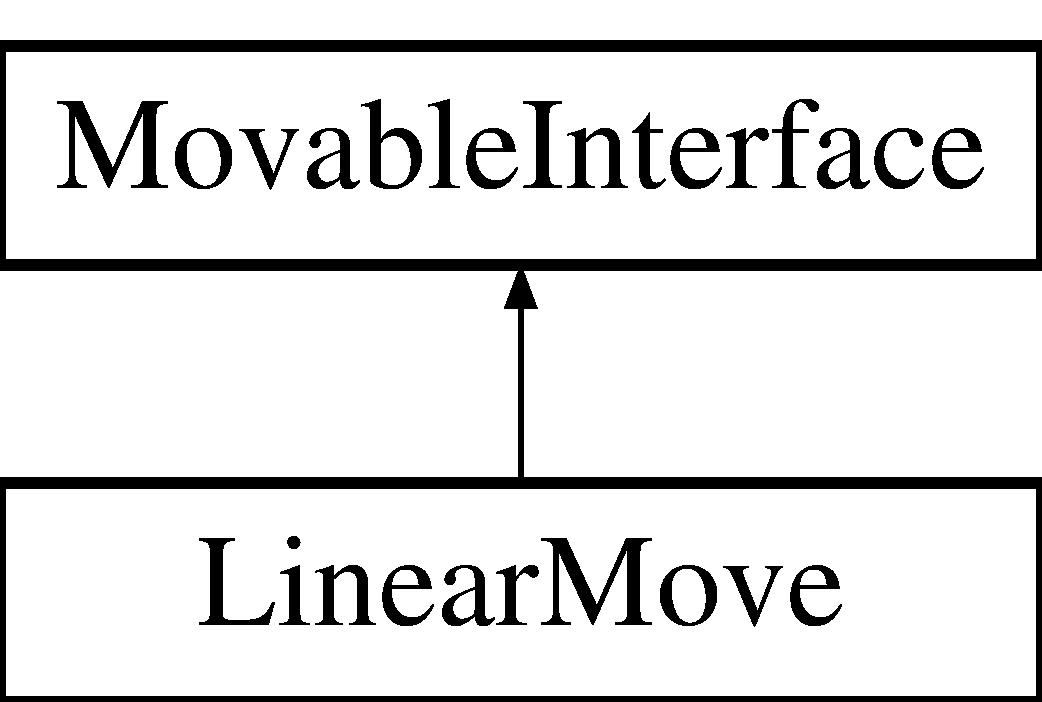
\includegraphics[height=2.000000cm]{df/d70/class_linear_move}
\end{center}
\end{figure}
\subsection*{Public Member Functions}
\begin{DoxyCompactItemize}
\item 
\hyperlink{class_linear_move_aa519e010d95eaaa372d3a45ba873d715}{Linear\+Move} (double move\+Speed)
\begin{DoxyCompactList}\small\item\em Constructs the object with a desired movement speed. \end{DoxyCompactList}\item 
virtual void \hyperlink{class_linear_move_a3a7b76828adfaefaaf7b687be499709d}{Move} (\hyperlink{class_vector2_d}{Vector2D} \&current\+Position) override
\begin{DoxyCompactList}\small\item\em Increases the \hyperlink{class_vector2_d}{Vector2D} that is passed in by reference along the straight line defined by the direction. \end{DoxyCompactList}\end{DoxyCompactItemize}
\subsection*{Additional Inherited Members}


\subsection{Detailed Description}
A basic implementation of the \hyperlink{class_movable_interface}{Movable\+Interface}, causes an object to move in a straight line along a specific direction. 

\subsection{Constructor \& Destructor Documentation}
\mbox{\Hypertarget{class_linear_move_aa519e010d95eaaa372d3a45ba873d715}\label{class_linear_move_aa519e010d95eaaa372d3a45ba873d715}} 
\index{Linear\+Move@{Linear\+Move}!Linear\+Move@{Linear\+Move}}
\index{Linear\+Move@{Linear\+Move}!Linear\+Move@{Linear\+Move}}
\subsubsection{\texorpdfstring{Linear\+Move()}{LinearMove()}}
{\footnotesize\ttfamily Linear\+Move\+::\+Linear\+Move (\begin{DoxyParamCaption}\item[{double}]{move\+Speed }\end{DoxyParamCaption})\hspace{0.3cm}{\ttfamily [inline]}}



Constructs the object with a desired movement speed. 


\begin{DoxyParams}{Parameters}
{\em move\+Speed} & the objects desired movespeed \\
\hline
\end{DoxyParams}


\subsection{Member Function Documentation}
\mbox{\Hypertarget{class_linear_move_a3a7b76828adfaefaaf7b687be499709d}\label{class_linear_move_a3a7b76828adfaefaaf7b687be499709d}} 
\index{Linear\+Move@{Linear\+Move}!Move@{Move}}
\index{Move@{Move}!Linear\+Move@{Linear\+Move}}
\subsubsection{\texorpdfstring{Move()}{Move()}}
{\footnotesize\ttfamily void Linear\+Move\+::\+Move (\begin{DoxyParamCaption}\item[{\hyperlink{class_vector2_d}{Vector2D} \&}]{current\+Position }\end{DoxyParamCaption})\hspace{0.3cm}{\ttfamily [override]}, {\ttfamily [virtual]}}



Increases the \hyperlink{class_vector2_d}{Vector2D} that is passed in by reference along the straight line defined by the direction. 


\begin{DoxyParams}{Parameters}
{\em current\+Position} & the current position that is adjusted \\
\hline
\end{DoxyParams}


Implements \hyperlink{class_movable_interface_a899cc1c78eacbee13b906c6770e7f025}{Movable\+Interface}.



The documentation for this class was generated from the following files\+:\begin{DoxyCompactItemize}
\item 
D\+:/\+Users/\+Tim-\/\+P\+C/\+Documents/\+Software\+\_\+\+I\+I/\+Project/\+Project\+Files/game-\/source-\/code/\+Front\+End\+Systems/Linear\+Move.\+h\item 
D\+:/\+Users/\+Tim-\/\+P\+C/\+Documents/\+Software\+\_\+\+I\+I/\+Project/\+Project\+Files/game-\/source-\/code/\+Front\+End\+Systems/Linear\+Move.\+cpp\end{DoxyCompactItemize}

\hypertarget{class_lose_scene_factory}{}\section{Lose\+Scene\+Factory Class Reference}
\label{class_lose_scene_factory}\index{Lose\+Scene\+Factory@{Lose\+Scene\+Factory}}


Creates the \hyperlink{class_scene}{Scene} that is displayed when the player loses the game.  




{\ttfamily \#include $<$Lose\+Scene\+Factory.\+h$>$}

Inheritance diagram for Lose\+Scene\+Factory\+:\begin{figure}[H]
\begin{center}
\leavevmode
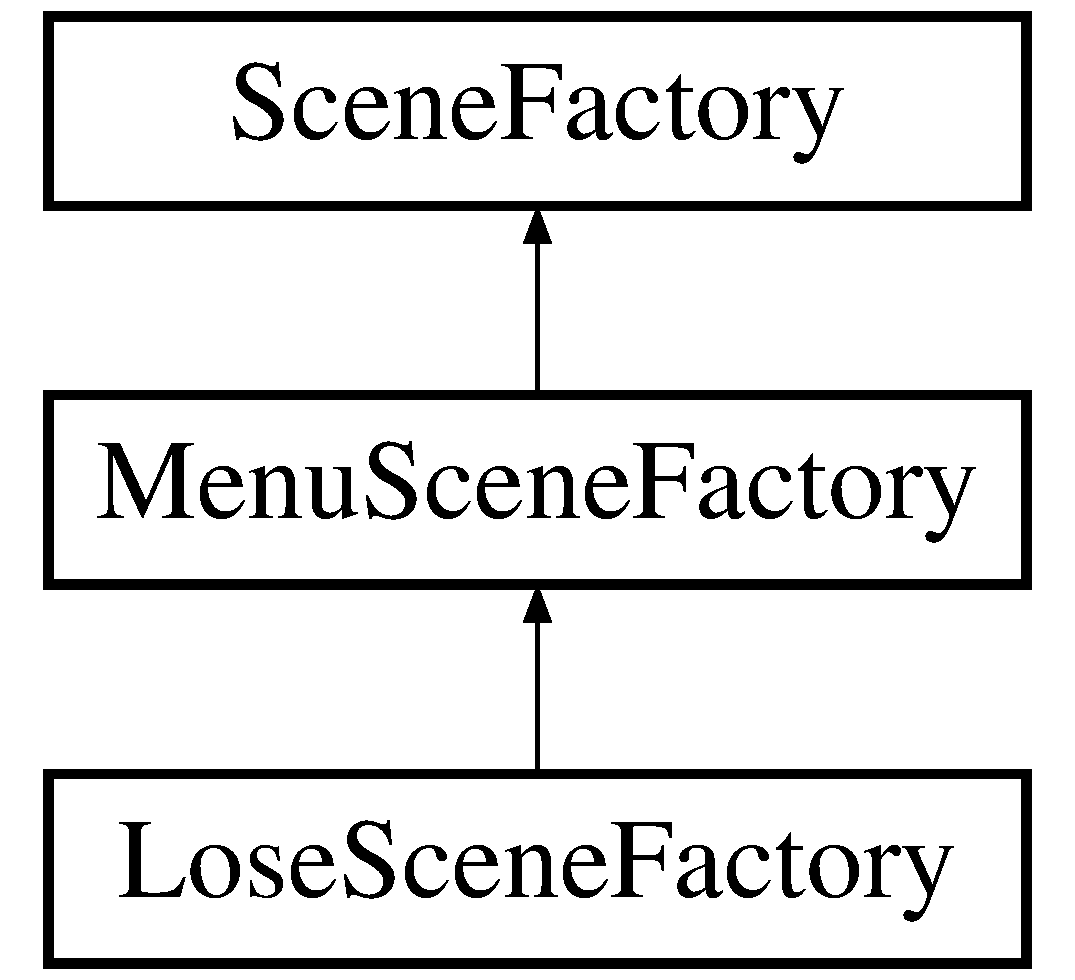
\includegraphics[height=3.000000cm]{dd/d0c/class_lose_scene_factory}
\end{center}
\end{figure}
\subsection*{Protected Member Functions}
\begin{DoxyCompactItemize}
\item 
\mbox{\Hypertarget{class_lose_scene_factory_adfe18ba674cdd988bb78e3cd3218796f}\label{class_lose_scene_factory_adfe18ba674cdd988bb78e3cd3218796f}} 
virtual std\+::shared\+\_\+ptr$<$ \hyperlink{class_background_factory}{Background\+Factory} $>$ {\bfseries get\+Factory} () const override
\end{DoxyCompactItemize}
\subsection*{Additional Inherited Members}


\subsection{Detailed Description}
Creates the \hyperlink{class_scene}{Scene} that is displayed when the player loses the game. 

The documentation for this class was generated from the following file\+:\begin{DoxyCompactItemize}
\item 
D\+:/\+Users/\+Tim-\/\+P\+C/\+Documents/\+Software\+\_\+\+I\+I/\+Project/\+Project\+Files/game-\/source-\/code/\+Back\+End\+Systems/Lose\+Scene\+Factory.\+h\end{DoxyCompactItemize}

\hypertarget{class_menu_scene_factory}{}\section{Menu\+Scene\+Factory Class Reference}
\label{class_menu_scene_factory}\index{Menu\+Scene\+Factory@{Menu\+Scene\+Factory}}


Creates the various Menu\+Scenes within the game.  




{\ttfamily \#include $<$Menu\+Scene\+Factory.\+h$>$}

Inheritance diagram for Menu\+Scene\+Factory\+:\begin{figure}[H]
\begin{center}
\leavevmode
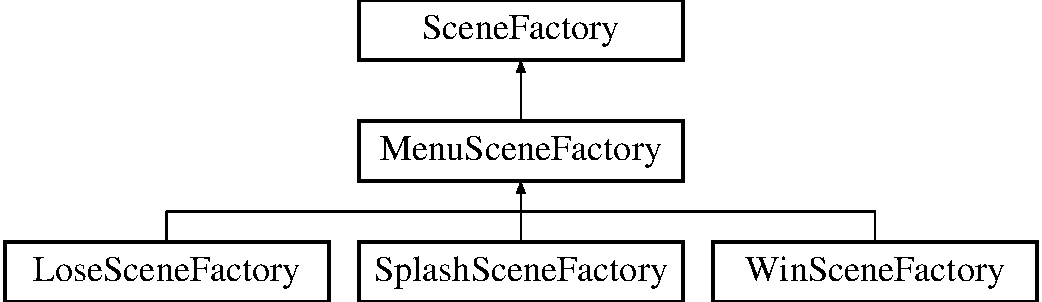
\includegraphics[height=3.000000cm]{da/d10/class_menu_scene_factory}
\end{center}
\end{figure}
\subsection*{Protected Member Functions}
\begin{DoxyCompactItemize}
\item 
virtual std\+::list$<$ std\+::shared\+\_\+ptr$<$ \hyperlink{class_game_object}{Game\+Object} $>$ $>$ \hyperlink{class_menu_scene_factory_ade1881c377fa61d1d8fa11c1d30f4ddd}{get\+Game\+Obect\+List} (std\+::shared\+\_\+ptr$<$ \hyperlink{class_database_interface}{Database\+Interface} $>$ database) const final
\begin{DoxyCompactList}\small\item\em Returns the game\+Object list required for the construction of the specific \hyperlink{class_scene}{Scene}. \end{DoxyCompactList}\item 
\mbox{\Hypertarget{class_menu_scene_factory_ad0f60a16fdbb10c6d7ba3311dafa2e76}\label{class_menu_scene_factory_ad0f60a16fdbb10c6d7ba3311dafa2e76}} 
virtual std\+::shared\+\_\+ptr$<$ \hyperlink{class_background_factory}{Background\+Factory} $>$ {\bfseries get\+Factory} () const =0
\end{DoxyCompactItemize}
\subsection*{Additional Inherited Members}


\subsection{Detailed Description}
Creates the various Menu\+Scenes within the game. 

\subsection{Member Function Documentation}
\mbox{\Hypertarget{class_menu_scene_factory_ade1881c377fa61d1d8fa11c1d30f4ddd}\label{class_menu_scene_factory_ade1881c377fa61d1d8fa11c1d30f4ddd}} 
\index{Menu\+Scene\+Factory@{Menu\+Scene\+Factory}!get\+Game\+Obect\+List@{get\+Game\+Obect\+List}}
\index{get\+Game\+Obect\+List@{get\+Game\+Obect\+List}!Menu\+Scene\+Factory@{Menu\+Scene\+Factory}}
\subsubsection{\texorpdfstring{get\+Game\+Obect\+List()}{getGameObectList()}}
{\footnotesize\ttfamily std\+::list$<$ std\+::shared\+\_\+ptr$<$ \hyperlink{class_game_object}{Game\+Object} $>$ $>$ Menu\+Scene\+Factory\+::get\+Game\+Obect\+List (\begin{DoxyParamCaption}\item[{std\+::shared\+\_\+ptr$<$ \hyperlink{class_database_interface}{Database\+Interface} $>$}]{database }\end{DoxyParamCaption}) const\hspace{0.3cm}{\ttfamily [final]}, {\ttfamily [protected]}, {\ttfamily [virtual]}}



Returns the game\+Object list required for the construction of the specific \hyperlink{class_scene}{Scene}. 


\begin{DoxyParams}{Parameters}
{\em database} & The \hyperlink{class_database_interface}{Database\+Interface} that contains the information about the various Game\+Objects \\
\hline
\end{DoxyParams}


Implements \hyperlink{class_scene_factory_a2c8541230e95df49d2ab39b7c6ecdb78}{Scene\+Factory}.



The documentation for this class was generated from the following files\+:\begin{DoxyCompactItemize}
\item 
D\+:/\+Users/\+Tim-\/\+P\+C/\+Documents/\+Software\+\_\+\+I\+I/\+Project/\+Project\+Files/game-\/source-\/code/\+Back\+End\+Systems/Menu\+Scene\+Factory.\+h\item 
D\+:/\+Users/\+Tim-\/\+P\+C/\+Documents/\+Software\+\_\+\+I\+I/\+Project/\+Project\+Files/game-\/source-\/code/\+Back\+End\+Systems/Menu\+Scene\+Factory.\+cpp\end{DoxyCompactItemize}

\hypertarget{class_movable_interface}{}\section{Movable\+Interface Class Reference}
\label{class_movable_interface}\index{Movable\+Interface@{Movable\+Interface}}


Defines the interfaces for any Movable\+Object Compositions.  




{\ttfamily \#include $<$Movable\+Interface.\+h$>$}

Inheritance diagram for Movable\+Interface\+:\begin{figure}[H]
\begin{center}
\leavevmode
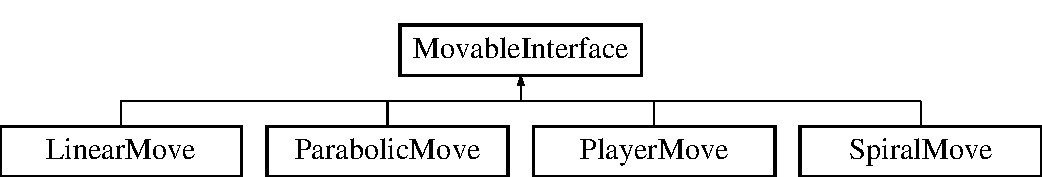
\includegraphics[height=2.000000cm]{dd/d92/class_movable_interface}
\end{center}
\end{figure}
\subsection*{Public Member Functions}
\begin{DoxyCompactItemize}
\item 
\hyperlink{class_movable_interface_a480a181d92f826515483b8ba57e4f030}{Movable\+Interface} (double move\+Speed)
\begin{DoxyCompactList}\small\item\em Constructor used to identify the move\+Speed of the object, direction is defaulted to right. \end{DoxyCompactList}\item 
virtual void \hyperlink{class_movable_interface_a899cc1c78eacbee13b906c6770e7f025}{Move} (\hyperlink{class_vector2_d}{Vector2D} \&current\+Position)=0
\begin{DoxyCompactList}\small\item\em Changes the \hyperlink{class_vector2_d}{Vector2D} that is passed in by reference to the appropriate value determined by the implementation. \end{DoxyCompactList}\item 
void \hyperlink{class_movable_interface_ac03895780649f51c762907e8ef3a7694}{set\+Direction} (const \hyperlink{class_vector2_d}{Vector2D} \&direction)
\begin{DoxyCompactList}\small\item\em Sets the direction to a specific value. \end{DoxyCompactList}\end{DoxyCompactItemize}
\subsection*{Protected Attributes}
\begin{DoxyCompactItemize}
\item 
double \hyperlink{class_movable_interface_aa9715fd066607de7e71ee7f891ae1dbd}{\+\_\+movespeed}
\item 
\hyperlink{class_vector2_d}{Vector2D} \hyperlink{class_movable_interface_aea3e1edf8c32ebe5fd37dc02d659c10d}{\+\_\+direction}
\end{DoxyCompactItemize}


\subsection{Detailed Description}
Defines the interfaces for any Movable\+Object Compositions. 

\subsection{Constructor \& Destructor Documentation}
\mbox{\Hypertarget{class_movable_interface_a480a181d92f826515483b8ba57e4f030}\label{class_movable_interface_a480a181d92f826515483b8ba57e4f030}} 
\index{Movable\+Interface@{Movable\+Interface}!Movable\+Interface@{Movable\+Interface}}
\index{Movable\+Interface@{Movable\+Interface}!Movable\+Interface@{Movable\+Interface}}
\subsubsection{\texorpdfstring{Movable\+Interface()}{MovableInterface()}}
{\footnotesize\ttfamily Movable\+Interface\+::\+Movable\+Interface (\begin{DoxyParamCaption}\item[{double}]{move\+Speed }\end{DoxyParamCaption})\hspace{0.3cm}{\ttfamily [inline]}}



Constructor used to identify the move\+Speed of the object, direction is defaulted to right. 


\begin{DoxyParams}{Parameters}
{\em move\+Speed} & \\
\hline
\end{DoxyParams}


\subsection{Member Function Documentation}
\mbox{\Hypertarget{class_movable_interface_a899cc1c78eacbee13b906c6770e7f025}\label{class_movable_interface_a899cc1c78eacbee13b906c6770e7f025}} 
\index{Movable\+Interface@{Movable\+Interface}!Move@{Move}}
\index{Move@{Move}!Movable\+Interface@{Movable\+Interface}}
\subsubsection{\texorpdfstring{Move()}{Move()}}
{\footnotesize\ttfamily virtual void Movable\+Interface\+::\+Move (\begin{DoxyParamCaption}\item[{\hyperlink{class_vector2_d}{Vector2D} \&}]{current\+Position }\end{DoxyParamCaption})\hspace{0.3cm}{\ttfamily [pure virtual]}}



Changes the \hyperlink{class_vector2_d}{Vector2D} that is passed in by reference to the appropriate value determined by the implementation. 


\begin{DoxyParams}{Parameters}
{\em current\+Position} & the current position that is adjusted \\
\hline
\end{DoxyParams}


Implemented in \hyperlink{class_linear_move_a3a7b76828adfaefaaf7b687be499709d}{Linear\+Move}, \hyperlink{class_player_move_a1c39885d4126c63441250eae23ac718a}{Player\+Move}, \hyperlink{class_spiral_move_a74b22995f5f3c00c623ecaa3adb2ab8e}{Spiral\+Move}, and \hyperlink{class_parabolic_move_a577831644247ca57aa1c2c88843c779b}{Parabolic\+Move}.

\mbox{\Hypertarget{class_movable_interface_ac03895780649f51c762907e8ef3a7694}\label{class_movable_interface_ac03895780649f51c762907e8ef3a7694}} 
\index{Movable\+Interface@{Movable\+Interface}!set\+Direction@{set\+Direction}}
\index{set\+Direction@{set\+Direction}!Movable\+Interface@{Movable\+Interface}}
\subsubsection{\texorpdfstring{set\+Direction()}{setDirection()}}
{\footnotesize\ttfamily void Movable\+Interface\+::set\+Direction (\begin{DoxyParamCaption}\item[{const \hyperlink{class_vector2_d}{Vector2D} \&}]{direction }\end{DoxyParamCaption})\hspace{0.3cm}{\ttfamily [inline]}}



Sets the direction to a specific value. 


\begin{DoxyParams}{Parameters}
{\em direction} & the desired direction \\
\hline
\end{DoxyParams}


\subsection{Member Data Documentation}
\mbox{\Hypertarget{class_movable_interface_aea3e1edf8c32ebe5fd37dc02d659c10d}\label{class_movable_interface_aea3e1edf8c32ebe5fd37dc02d659c10d}} 
\index{Movable\+Interface@{Movable\+Interface}!\+\_\+direction@{\+\_\+direction}}
\index{\+\_\+direction@{\+\_\+direction}!Movable\+Interface@{Movable\+Interface}}
\subsubsection{\texorpdfstring{\+\_\+direction}{\_direction}}
{\footnotesize\ttfamily \hyperlink{class_vector2_d}{Vector2D} Movable\+Interface\+::\+\_\+direction\hspace{0.3cm}{\ttfamily [protected]}}

The direction that the object moves in \mbox{\Hypertarget{class_movable_interface_aa9715fd066607de7e71ee7f891ae1dbd}\label{class_movable_interface_aa9715fd066607de7e71ee7f891ae1dbd}} 
\index{Movable\+Interface@{Movable\+Interface}!\+\_\+movespeed@{\+\_\+movespeed}}
\index{\+\_\+movespeed@{\+\_\+movespeed}!Movable\+Interface@{Movable\+Interface}}
\subsubsection{\texorpdfstring{\+\_\+movespeed}{\_movespeed}}
{\footnotesize\ttfamily double Movable\+Interface\+::\+\_\+movespeed\hspace{0.3cm}{\ttfamily [protected]}}

The movement speed of the object 

The documentation for this class was generated from the following file\+:\begin{DoxyCompactItemize}
\item 
C\+:/\+Users/\+Tim/\+Documents/\+Software\+Dev/\+Software\+Project/\+Project\+Files/game-\/source-\/code/\+Front\+End\+Systems/Movable\+Interface.\+h\end{DoxyCompactItemize}

\hypertarget{class_non_projectile_object_shot}{}\section{Non\+Projectile\+Object\+Shot Class Reference}
\label{class_non_projectile_object_shot}\index{Non\+Projectile\+Object\+Shot@{Non\+Projectile\+Object\+Shot}}


Exception thrown if an object that doesnt derive from \hyperlink{class_projectile}{Projectile} is used.  




{\ttfamily \#include $<$Basic\+Shoot.\+h$>$}



\subsection{Detailed Description}
Exception thrown if an object that doesnt derive from \hyperlink{class_projectile}{Projectile} is used. 

The documentation for this class was generated from the following file\+:\begin{DoxyCompactItemize}
\item 
D\+:/\+Users/\+Tim-\/\+P\+C/\+Documents/\+Software\+\_\+\+I\+I/\+Project/\+Project\+Files/game-\/source-\/code/\+Front\+End\+Systems/Basic\+Shoot.\+h\end{DoxyCompactItemize}

\hypertarget{class_parabolic_enemy_factory}{}\section{Parabolic\+Enemy\+Factory Class Reference}
\label{class_parabolic_enemy_factory}\index{Parabolic\+Enemy\+Factory@{Parabolic\+Enemy\+Factory}}


Constructs an \hyperlink{class_enemy}{Enemy} that is moves in a parabolic fashion from the edges of the screen to the centre of the screen.  




{\ttfamily \#include $<$Parabolic\+Enemy\+Factory.\+h$>$}

Inheritance diagram for Parabolic\+Enemy\+Factory\+:\begin{figure}[H]
\begin{center}
\leavevmode
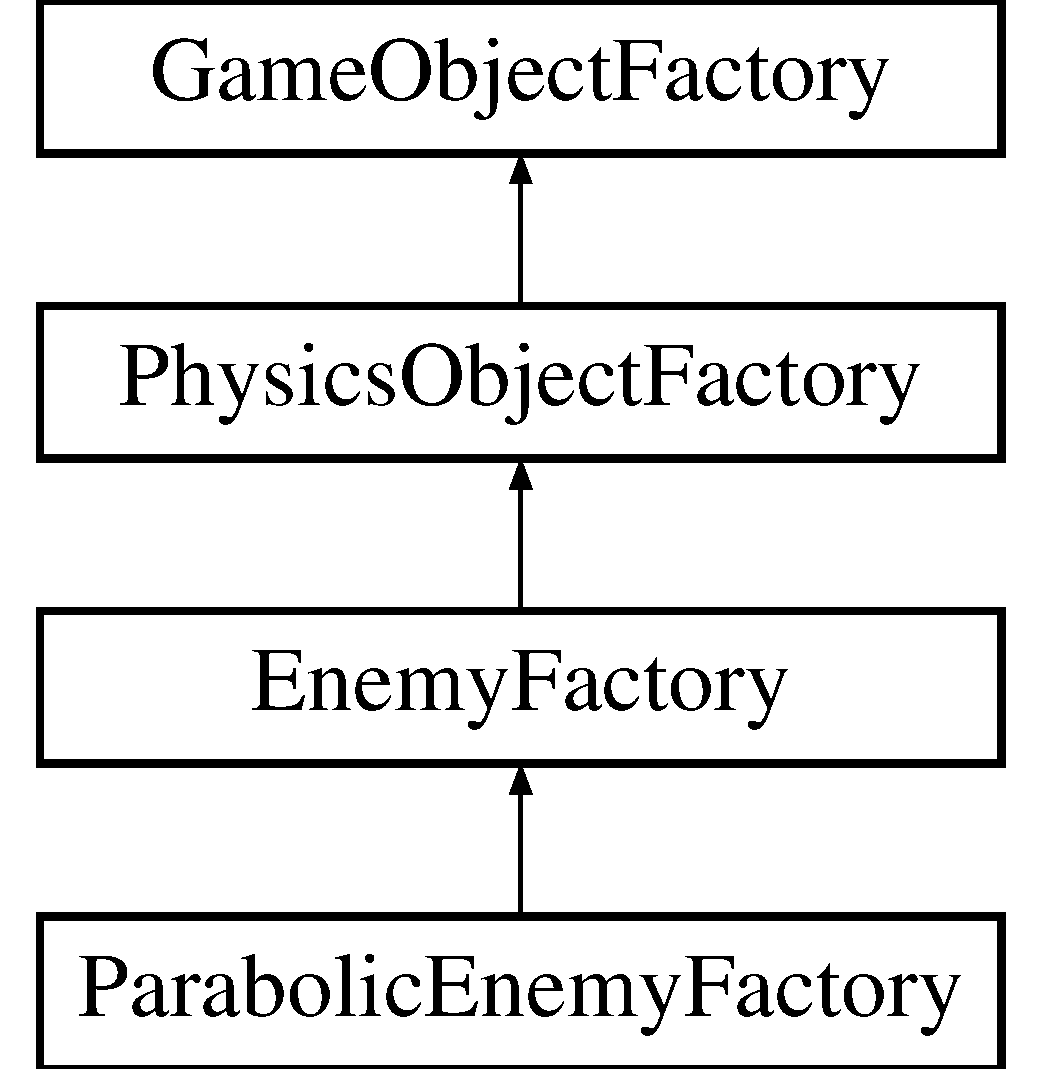
\includegraphics[height=4.000000cm]{db/d73/class_parabolic_enemy_factory}
\end{center}
\end{figure}
\subsection*{Public Member Functions}
\begin{DoxyCompactItemize}
\item 
virtual std\+::shared\+\_\+ptr$<$ \hyperlink{class_movable_interface}{Movable\+Interface} $>$ \hyperlink{class_parabolic_enemy_factory_aaf1f3323e4c723f669a11c20a7e38efe}{get\+Movable\+Type} (const \hyperlink{struct_game_object_data}{Game\+Object\+Data} \&data) override
\begin{DoxyCompactList}\small\item\em Pure virtual function used to assign the various Movable\+Interfaces that the Enemy\+Objects use. \end{DoxyCompactList}\item 
virtual \hyperlink{struct_game_object_data}{Game\+Object\+Data} \hyperlink{class_parabolic_enemy_factory_acc62c48a8eb5af162910dc48d9fe8900}{get\+Object\+Data} (const std\+::shared\+\_\+ptr$<$ \hyperlink{class_database_interface}{Database\+Interface} $>$ \&database) override
\begin{DoxyCompactList}\small\item\em used to obtain the specific \hyperlink{struct_game_object_data}{Game\+Object\+Data} defined for the current factory \end{DoxyCompactList}\end{DoxyCompactItemize}
\subsection*{Private Member Functions}
\begin{DoxyCompactItemize}
\item 
\mbox{\Hypertarget{class_parabolic_enemy_factory_ad94922df9b01d26e5d7fda695dcc41a5}\label{class_parabolic_enemy_factory_ad94922df9b01d26e5d7fda695dcc41a5}} 
double {\bfseries determine\+Parabolic\+Coefficient} ()
\end{DoxyCompactItemize}


\subsection{Detailed Description}
Constructs an \hyperlink{class_enemy}{Enemy} that is moves in a parabolic fashion from the edges of the screen to the centre of the screen. 

\subsection{Member Function Documentation}
\mbox{\Hypertarget{class_parabolic_enemy_factory_aaf1f3323e4c723f669a11c20a7e38efe}\label{class_parabolic_enemy_factory_aaf1f3323e4c723f669a11c20a7e38efe}} 
\index{Parabolic\+Enemy\+Factory@{Parabolic\+Enemy\+Factory}!get\+Movable\+Type@{get\+Movable\+Type}}
\index{get\+Movable\+Type@{get\+Movable\+Type}!Parabolic\+Enemy\+Factory@{Parabolic\+Enemy\+Factory}}
\subsubsection{\texorpdfstring{get\+Movable\+Type()}{getMovableType()}}
{\footnotesize\ttfamily std\+::shared\+\_\+ptr$<$ \hyperlink{class_movable_interface}{Movable\+Interface} $>$ Parabolic\+Enemy\+Factory\+::get\+Movable\+Type (\begin{DoxyParamCaption}\item[{const \hyperlink{struct_game_object_data}{Game\+Object\+Data} \&}]{data }\end{DoxyParamCaption})\hspace{0.3cm}{\ttfamily [override]}, {\ttfamily [virtual]}}



Pure virtual function used to assign the various Movable\+Interfaces that the Enemy\+Objects use. 


\begin{DoxyParams}{Parameters}
{\em data} & The \hyperlink{struct_game_object_data}{Game\+Object\+Data} specific to the \hyperlink{class_enemy}{Enemy} being constructed \\
\hline
\end{DoxyParams}
\begin{DoxyReturn}{Returns}
Returns the \hyperlink{class_movable_interface}{Movable\+Interface} for the specific \hyperlink{class_enemy}{Enemy} that is being constructed 
\end{DoxyReturn}


Implements \hyperlink{class_enemy_factory_ae064082d650e676960cb84ebb60ba216}{Enemy\+Factory}.

\mbox{\Hypertarget{class_parabolic_enemy_factory_acc62c48a8eb5af162910dc48d9fe8900}\label{class_parabolic_enemy_factory_acc62c48a8eb5af162910dc48d9fe8900}} 
\index{Parabolic\+Enemy\+Factory@{Parabolic\+Enemy\+Factory}!get\+Object\+Data@{get\+Object\+Data}}
\index{get\+Object\+Data@{get\+Object\+Data}!Parabolic\+Enemy\+Factory@{Parabolic\+Enemy\+Factory}}
\subsubsection{\texorpdfstring{get\+Object\+Data()}{getObjectData()}}
{\footnotesize\ttfamily \hyperlink{struct_game_object_data}{Game\+Object\+Data} Parabolic\+Enemy\+Factory\+::get\+Object\+Data (\begin{DoxyParamCaption}\item[{const std\+::shared\+\_\+ptr$<$ \hyperlink{class_database_interface}{Database\+Interface} $>$ \&}]{database }\end{DoxyParamCaption})\hspace{0.3cm}{\ttfamily [override]}, {\ttfamily [virtual]}}



used to obtain the specific \hyperlink{struct_game_object_data}{Game\+Object\+Data} defined for the current factory 


\begin{DoxyParams}{Parameters}
{\em database} & The specific \hyperlink{class_database_interface}{Database\+Interface} that contains the information about the Game\+Objects \\
\hline
\end{DoxyParams}
\begin{DoxyReturn}{Returns}
The \hyperlink{struct_game_object_data}{Game\+Object\+Data} required for the construction of the object 
\end{DoxyReturn}


Implements \hyperlink{class_physics_object_factory_aa59f52d3adc1fac676f4a8a3c2de9ba9}{Physics\+Object\+Factory}.



The documentation for this class was generated from the following files\+:\begin{DoxyCompactItemize}
\item 
C\+:/\+Users/\+Tim/\+Documents/\+Software\+Dev/\+Software\+Project/\+Project\+Files/game-\/source-\/code/\+Back\+End\+Systems/Parabolic\+Enemy\+Factory.\+h\item 
C\+:/\+Users/\+Tim/\+Documents/\+Software\+Dev/\+Software\+Project/\+Project\+Files/game-\/source-\/code/\+Back\+End\+Systems/Parabolic\+Enemy\+Factory.\+cpp\end{DoxyCompactItemize}

\hypertarget{class_parabolic_move}{}\section{Parabolic\+Move Class Reference}
\label{class_parabolic_move}\index{Parabolic\+Move@{Parabolic\+Move}}


Complex movement pattern which causes an position to change in a parabolic shape through the origin.  




{\ttfamily \#include $<$Parabolic\+Move.\+h$>$}

Inheritance diagram for Parabolic\+Move\+:\begin{figure}[H]
\begin{center}
\leavevmode
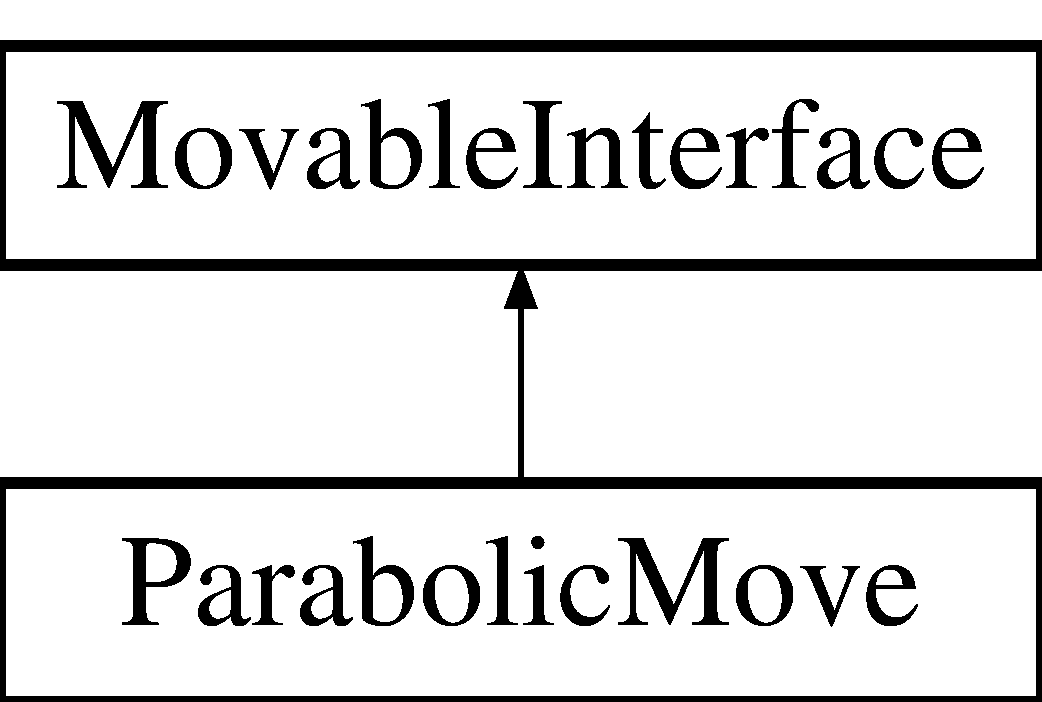
\includegraphics[height=2.000000cm]{d3/da6/class_parabolic_move}
\end{center}
\end{figure}
\subsection*{Public Member Functions}
\begin{DoxyCompactItemize}
\item 
\hyperlink{class_parabolic_move_a94fb02788b26d03abccee8254401902d}{Parabolic\+Move} (const double \&parabolic\+\_\+coefficient, const double \&movespeed)
\begin{DoxyCompactList}\small\item\em Constructs a \hyperlink{class_parabolic_move}{Parabolic\+Move} Object with the specified parameters. \end{DoxyCompactList}\item 
virtual void \hyperlink{class_parabolic_move_a577831644247ca57aa1c2c88843c779b}{Move} (\hyperlink{class_vector2_d}{Vector2D} \&current\+Position) override
\begin{DoxyCompactList}\small\item\em varies the \hyperlink{class_vector2_d}{Vector2D} in a parabolic way, by using the equation of a parabola that passes through the origin \end{DoxyCompactList}\end{DoxyCompactItemize}
\subsection*{Private Member Functions}
\begin{DoxyCompactItemize}
\item 
double \hyperlink{class_parabolic_move_a1fde73a6298c970648344e0e232659d5}{Move\+Speed} (const \hyperlink{class_vector2_d}{Vector2D} \&position)
\begin{DoxyCompactList}\small\item\em Determines the movespeed of the object based on its proximity to the origin. \end{DoxyCompactList}\end{DoxyCompactItemize}
\subsection*{Private Attributes}
\begin{DoxyCompactItemize}
\item 
double \hyperlink{class_parabolic_move_a4ae7c298df76cb1a0f5f7d6f85c0977c}{\+\_\+parabolic\+\_\+coefficient}
\end{DoxyCompactItemize}
\subsection*{Additional Inherited Members}


\subsection{Detailed Description}
Complex movement pattern which causes an position to change in a parabolic shape through the origin. 

\subsection{Constructor \& Destructor Documentation}
\mbox{\Hypertarget{class_parabolic_move_a94fb02788b26d03abccee8254401902d}\label{class_parabolic_move_a94fb02788b26d03abccee8254401902d}} 
\index{Parabolic\+Move@{Parabolic\+Move}!Parabolic\+Move@{Parabolic\+Move}}
\index{Parabolic\+Move@{Parabolic\+Move}!Parabolic\+Move@{Parabolic\+Move}}
\subsubsection{\texorpdfstring{Parabolic\+Move()}{ParabolicMove()}}
{\footnotesize\ttfamily Parabolic\+Move\+::\+Parabolic\+Move (\begin{DoxyParamCaption}\item[{const double \&}]{parabolic\+\_\+coefficient,  }\item[{const double \&}]{movespeed }\end{DoxyParamCaption})}



Constructs a \hyperlink{class_parabolic_move}{Parabolic\+Move} Object with the specified parameters. 


\begin{DoxyParams}{Parameters}
{\em parabolic\+\_\+coefficient} & the desired coefficient value used to determine the spread of the parabola \\
\hline
{\em movespeed} & the movement speed used to determine how fast a position changes \\
\hline
\end{DoxyParams}


\subsection{Member Function Documentation}
\mbox{\Hypertarget{class_parabolic_move_a577831644247ca57aa1c2c88843c779b}\label{class_parabolic_move_a577831644247ca57aa1c2c88843c779b}} 
\index{Parabolic\+Move@{Parabolic\+Move}!Move@{Move}}
\index{Move@{Move}!Parabolic\+Move@{Parabolic\+Move}}
\subsubsection{\texorpdfstring{Move()}{Move()}}
{\footnotesize\ttfamily void Parabolic\+Move\+::\+Move (\begin{DoxyParamCaption}\item[{\hyperlink{class_vector2_d}{Vector2D} \&}]{current\+Position }\end{DoxyParamCaption})\hspace{0.3cm}{\ttfamily [override]}, {\ttfamily [virtual]}}



varies the \hyperlink{class_vector2_d}{Vector2D} in a parabolic way, by using the equation of a parabola that passes through the origin 


\begin{DoxyParams}{Parameters}
{\em current\+Position} & \\
\hline
\end{DoxyParams}


Implements \hyperlink{class_movable_interface_a899cc1c78eacbee13b906c6770e7f025}{Movable\+Interface}.

\mbox{\Hypertarget{class_parabolic_move_a1fde73a6298c970648344e0e232659d5}\label{class_parabolic_move_a1fde73a6298c970648344e0e232659d5}} 
\index{Parabolic\+Move@{Parabolic\+Move}!Move\+Speed@{Move\+Speed}}
\index{Move\+Speed@{Move\+Speed}!Parabolic\+Move@{Parabolic\+Move}}
\subsubsection{\texorpdfstring{Move\+Speed()}{MoveSpeed()}}
{\footnotesize\ttfamily double Parabolic\+Move\+::\+Move\+Speed (\begin{DoxyParamCaption}\item[{const \hyperlink{class_vector2_d}{Vector2D} \&}]{position }\end{DoxyParamCaption})\hspace{0.3cm}{\ttfamily [private]}}



Determines the movespeed of the object based on its proximity to the origin. 


\begin{DoxyParams}{Parameters}
{\em position} & the current position of the object \\
\hline
\end{DoxyParams}
\begin{DoxyReturn}{Returns}
returns the determined movement speed of the object 
\end{DoxyReturn}


\subsection{Member Data Documentation}
\mbox{\Hypertarget{class_parabolic_move_a4ae7c298df76cb1a0f5f7d6f85c0977c}\label{class_parabolic_move_a4ae7c298df76cb1a0f5f7d6f85c0977c}} 
\index{Parabolic\+Move@{Parabolic\+Move}!\+\_\+parabolic\+\_\+coefficient@{\+\_\+parabolic\+\_\+coefficient}}
\index{\+\_\+parabolic\+\_\+coefficient@{\+\_\+parabolic\+\_\+coefficient}!Parabolic\+Move@{Parabolic\+Move}}
\subsubsection{\texorpdfstring{\+\_\+parabolic\+\_\+coefficient}{\_parabolic\_coefficient}}
{\footnotesize\ttfamily double Parabolic\+Move\+::\+\_\+parabolic\+\_\+coefficient\hspace{0.3cm}{\ttfamily [private]}}

The coeficient value used to determine the spread of the parabola 

The documentation for this class was generated from the following files\+:\begin{DoxyCompactItemize}
\item 
D\+:/\+Users/\+Tim-\/\+P\+C/\+Documents/\+Software\+\_\+\+I\+I/\+Project/\+Project\+Files/game-\/source-\/code/\+Front\+End\+Systems/Parabolic\+Move.\+h\item 
D\+:/\+Users/\+Tim-\/\+P\+C/\+Documents/\+Software\+\_\+\+I\+I/\+Project/\+Project\+Files/game-\/source-\/code/\+Front\+End\+Systems/Parabolic\+Move.\+cpp\end{DoxyCompactItemize}

\hypertarget{class_physics_object}{}\section{Physics\+Object Class Reference}
\label{class_physics_object}\index{Physics\+Object@{Physics\+Object}}


Acts as the main interface between the collision\+Detection and the game logic.  




{\ttfamily \#include $<$Physics\+Object.\+h$>$}

Inheritance diagram for Physics\+Object\+:\begin{figure}[H]
\begin{center}
\leavevmode
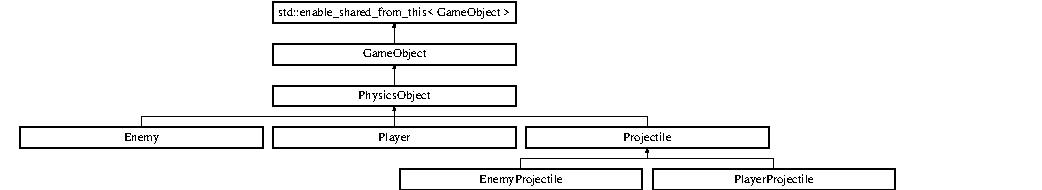
\includegraphics[height=2.527076cm]{d6/db5/class_physics_object}
\end{center}
\end{figure}
\subsection*{Public Member Functions}
\begin{DoxyCompactItemize}
\item 
\mbox{\Hypertarget{class_physics_object_a0dd37cc0f9535b676d3df937eaeb4780}\label{class_physics_object_a0dd37cc0f9535b676d3df937eaeb4780}} 
\hyperlink{class_physics_object_a0dd37cc0f9535b676d3df937eaeb4780}{Physics\+Object} ()
\begin{DoxyCompactList}\small\item\em Default Constructor. \end{DoxyCompactList}\item 
\hyperlink{class_physics_object_a8a92618716bd764c63f0ca80436a950c}{Physics\+Object} (const \hyperlink{class_game_object}{Game\+Object} \&game\+Object, const double \&object\+Size)
\begin{DoxyCompactList}\small\item\em Constructs the physics object based on the parameters provided. \end{DoxyCompactList}\item 
double \hyperlink{class_physics_object_adc592e9846ebedea3d58d50c5ada1c12}{get\+Size} () const
\begin{DoxyCompactList}\small\item\em gets the current size of the object \end{DoxyCompactList}\item 
virtual void \hyperlink{class_physics_object_a16163f4e5bf781b3814d024c9f44a276}{collision\+Action} (const Game\+Object\+Type \&object\+Type)
\begin{DoxyCompactList}\small\item\em Virtual function that is called whenever a collision occurs between this object and a different one. \end{DoxyCompactList}\end{DoxyCompactItemize}
\subsection*{Protected Attributes}
\begin{DoxyCompactItemize}
\item 
double \hyperlink{class_physics_object_a417a7eb051cfcfdbf8dfd0cc0875fa0d}{\+\_\+object\+Size}
\end{DoxyCompactItemize}
\subsection*{Additional Inherited Members}


\subsection{Detailed Description}
Acts as the main interface between the collision\+Detection and the game logic. 

Provides the size for the collision\+Detection to check as well as a function call for when a collision occurs. 

\subsection{Constructor \& Destructor Documentation}
\mbox{\Hypertarget{class_physics_object_a8a92618716bd764c63f0ca80436a950c}\label{class_physics_object_a8a92618716bd764c63f0ca80436a950c}} 
\index{Physics\+Object@{Physics\+Object}!Physics\+Object@{Physics\+Object}}
\index{Physics\+Object@{Physics\+Object}!Physics\+Object@{Physics\+Object}}
\subsubsection{\texorpdfstring{Physics\+Object()}{PhysicsObject()}}
{\footnotesize\ttfamily Physics\+Object\+::\+Physics\+Object (\begin{DoxyParamCaption}\item[{const \hyperlink{class_game_object}{Game\+Object} \&}]{game\+Object,  }\item[{const double \&}]{object\+Size }\end{DoxyParamCaption})}



Constructs the physics object based on the parameters provided. 


\begin{DoxyParams}{Parameters}
{\em game\+Object} & A copy of the gameobject is made and is applied to the object \\
\hline
{\em object\+Size} & The radial size of the object and its area of collision \\
\hline
\end{DoxyParams}


\subsection{Member Function Documentation}
\mbox{\Hypertarget{class_physics_object_a16163f4e5bf781b3814d024c9f44a276}\label{class_physics_object_a16163f4e5bf781b3814d024c9f44a276}} 
\index{Physics\+Object@{Physics\+Object}!collision\+Action@{collision\+Action}}
\index{collision\+Action@{collision\+Action}!Physics\+Object@{Physics\+Object}}
\subsubsection{\texorpdfstring{collision\+Action()}{collisionAction()}}
{\footnotesize\ttfamily void Physics\+Object\+::collision\+Action (\begin{DoxyParamCaption}\item[{const Game\+Object\+Type \&}]{object\+Type }\end{DoxyParamCaption})\hspace{0.3cm}{\ttfamily [virtual]}}



Virtual function that is called whenever a collision occurs between this object and a different one. 


\begin{DoxyParams}{Parameters}
{\em object\+Type} & The Game\+Object\+Type of the object that was collided with \\
\hline
\end{DoxyParams}


Reimplemented in \hyperlink{class_enemy_ac59660a58fac8d0ffdcb97c0717fa089}{Enemy}, \hyperlink{class_player_a1089079d7149a7fce6226935a6ce2f9c}{Player}, \hyperlink{class_player_projectile_a22fcdd7296d95b97ae60b4d20d8a57bd}{Player\+Projectile}, and \hyperlink{class_enemy_projectile_a4b3233a5ba7a3df66070cd6cdaa0362a}{Enemy\+Projectile}.

\mbox{\Hypertarget{class_physics_object_adc592e9846ebedea3d58d50c5ada1c12}\label{class_physics_object_adc592e9846ebedea3d58d50c5ada1c12}} 
\index{Physics\+Object@{Physics\+Object}!get\+Size@{get\+Size}}
\index{get\+Size@{get\+Size}!Physics\+Object@{Physics\+Object}}
\subsubsection{\texorpdfstring{get\+Size()}{getSize()}}
{\footnotesize\ttfamily double Physics\+Object\+::get\+Size (\begin{DoxyParamCaption}{ }\end{DoxyParamCaption}) const}



gets the current size of the object 

\begin{DoxyReturn}{Returns}
Returns the object size 
\end{DoxyReturn}


\subsection{Member Data Documentation}
\mbox{\Hypertarget{class_physics_object_a417a7eb051cfcfdbf8dfd0cc0875fa0d}\label{class_physics_object_a417a7eb051cfcfdbf8dfd0cc0875fa0d}} 
\index{Physics\+Object@{Physics\+Object}!\+\_\+object\+Size@{\+\_\+object\+Size}}
\index{\+\_\+object\+Size@{\+\_\+object\+Size}!Physics\+Object@{Physics\+Object}}
\subsubsection{\texorpdfstring{\+\_\+object\+Size}{\_objectSize}}
{\footnotesize\ttfamily double Physics\+Object\+::\+\_\+object\+Size\hspace{0.3cm}{\ttfamily [protected]}}

The radial collision size of the object 

The documentation for this class was generated from the following files\+:\begin{DoxyCompactItemize}
\item 
C\+:/\+Users/\+Tim/\+Documents/\+Software\+Dev/\+Software\+Project/\+Project\+Files/game-\/source-\/code/\+Front\+End\+Systems/Physics\+Object.\+h\item 
C\+:/\+Users/\+Tim/\+Documents/\+Software\+Dev/\+Software\+Project/\+Project\+Files/game-\/source-\/code/\+Front\+End\+Systems/Physics\+Object.\+cpp\end{DoxyCompactItemize}

\hypertarget{class_physics_object_factory}{}\section{Physics\+Object\+Factory Class Reference}
\label{class_physics_object_factory}\index{Physics\+Object\+Factory@{Physics\+Object\+Factory}}


Used to construct a physics Object within the game.  




{\ttfamily \#include $<$Physics\+Object\+Factory.\+h$>$}

Inheritance diagram for Physics\+Object\+Factory\+:\begin{figure}[H]
\begin{center}
\leavevmode
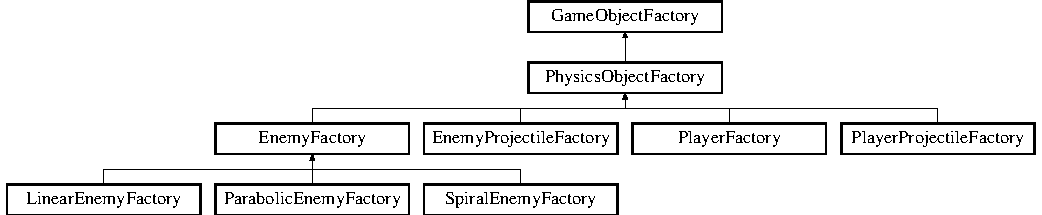
\includegraphics[height=2.871795cm]{de/dc7/class_physics_object_factory}
\end{center}
\end{figure}
\subsection*{Public Member Functions}
\begin{DoxyCompactItemize}
\item 
virtual std\+::shared\+\_\+ptr$<$ \hyperlink{class_game_object}{Game\+Object} $>$ \hyperlink{class_physics_object_factory_a2644107d0c455c3307559cd824a7c9a8}{get\+Game\+Object} (const std\+::shared\+\_\+ptr$<$ \hyperlink{class_database_interface}{Database\+Interface} $>$ \&database) override
\begin{DoxyCompactList}\small\item\em virtual function used to create the desired class specified by the derived class \end{DoxyCompactList}\item 
virtual \hyperlink{struct_game_object_data}{Game\+Object\+Data} \hyperlink{class_physics_object_factory_aa59f52d3adc1fac676f4a8a3c2de9ba9}{get\+Object\+Data} (const std\+::shared\+\_\+ptr$<$ \hyperlink{class_database_interface}{Database\+Interface} $>$ \&database) override=0
\begin{DoxyCompactList}\small\item\em used to obtain the specific \hyperlink{struct_game_object_data}{Game\+Object\+Data} defined for the current factory \end{DoxyCompactList}\end{DoxyCompactItemize}


\subsection{Detailed Description}
Used to construct a physics Object within the game. 

\subsection{Member Function Documentation}
\mbox{\Hypertarget{class_physics_object_factory_a2644107d0c455c3307559cd824a7c9a8}\label{class_physics_object_factory_a2644107d0c455c3307559cd824a7c9a8}} 
\index{Physics\+Object\+Factory@{Physics\+Object\+Factory}!get\+Game\+Object@{get\+Game\+Object}}
\index{get\+Game\+Object@{get\+Game\+Object}!Physics\+Object\+Factory@{Physics\+Object\+Factory}}
\subsubsection{\texorpdfstring{get\+Game\+Object()}{getGameObject()}}
{\footnotesize\ttfamily std\+::shared\+\_\+ptr$<$ \hyperlink{class_game_object}{Game\+Object} $>$ Physics\+Object\+Factory\+::get\+Game\+Object (\begin{DoxyParamCaption}\item[{const std\+::shared\+\_\+ptr$<$ \hyperlink{class_database_interface}{Database\+Interface} $>$ \&}]{database }\end{DoxyParamCaption})\hspace{0.3cm}{\ttfamily [override]}, {\ttfamily [virtual]}}



virtual function used to create the desired class specified by the derived class 

\begin{DoxyReturn}{Returns}
Returns the constructed \hyperlink{class_game_object}{Game\+Object} object 
\end{DoxyReturn}


Reimplemented from \hyperlink{class_game_object_factory_a5b684a6e77fb82c041f1721eb07c553d}{Game\+Object\+Factory}.



Reimplemented in \hyperlink{class_player_factory_ab92534e7d2d6887ecf9e4ed8131a8112}{Player\+Factory}, \hyperlink{class_enemy_factory_acb6ad18d5ef69a27927907fa9a444c7d}{Enemy\+Factory}, \hyperlink{class_enemy_projectile_factory_a081c6bea7032956c278fdf4ff62d530a}{Enemy\+Projectile\+Factory}, and \hyperlink{class_player_projectile_factory_a804a9f591ce6f0a7fb04f35ff685ff57}{Player\+Projectile\+Factory}.

\mbox{\Hypertarget{class_physics_object_factory_aa59f52d3adc1fac676f4a8a3c2de9ba9}\label{class_physics_object_factory_aa59f52d3adc1fac676f4a8a3c2de9ba9}} 
\index{Physics\+Object\+Factory@{Physics\+Object\+Factory}!get\+Object\+Data@{get\+Object\+Data}}
\index{get\+Object\+Data@{get\+Object\+Data}!Physics\+Object\+Factory@{Physics\+Object\+Factory}}
\subsubsection{\texorpdfstring{get\+Object\+Data()}{getObjectData()}}
{\footnotesize\ttfamily virtual \hyperlink{struct_game_object_data}{Game\+Object\+Data} Physics\+Object\+Factory\+::get\+Object\+Data (\begin{DoxyParamCaption}\item[{const std\+::shared\+\_\+ptr$<$ \hyperlink{class_database_interface}{Database\+Interface} $>$ \&}]{database }\end{DoxyParamCaption})\hspace{0.3cm}{\ttfamily [override]}, {\ttfamily [pure virtual]}}



used to obtain the specific \hyperlink{struct_game_object_data}{Game\+Object\+Data} defined for the current factory 


\begin{DoxyParams}{Parameters}
{\em database} & The specific \hyperlink{class_database_interface}{Database\+Interface} that contains the information about the Game\+Objects \\
\hline
\end{DoxyParams}
\begin{DoxyReturn}{Returns}
The \hyperlink{struct_game_object_data}{Game\+Object\+Data} required for the construction of the object 
\end{DoxyReturn}


Implements \hyperlink{class_game_object_factory_ae9358fbb3ef2d3b127320341760d3ff9}{Game\+Object\+Factory}.



Implemented in \hyperlink{class_enemy_projectile_factory_a1ef660e5962f29b7353054c6480477c7}{Enemy\+Projectile\+Factory}, \hyperlink{class_player_factory_aca4e809430541d77acd4c588c4381715}{Player\+Factory}, \hyperlink{class_player_projectile_factory_a702ae964c9dc653140fad4e17f38f60a}{Player\+Projectile\+Factory}, \hyperlink{class_parabolic_enemy_factory_acc62c48a8eb5af162910dc48d9fe8900}{Parabolic\+Enemy\+Factory}, \hyperlink{class_spiral_enemy_factory_a230709a0781c4364aa062b0bd441ec4d}{Spiral\+Enemy\+Factory}, and \hyperlink{class_linear_enemy_factory_a9d959b8a414e30ad4813d5d3740eafee}{Linear\+Enemy\+Factory}.



The documentation for this class was generated from the following files\+:\begin{DoxyCompactItemize}
\item 
C\+:/\+Users/\+Tim/\+Documents/\+Software\+Dev/\+Software\+Project/\+Project\+Files/game-\/source-\/code/\+Back\+End\+Systems/Physics\+Object\+Factory.\+h\item 
C\+:/\+Users/\+Tim/\+Documents/\+Software\+Dev/\+Software\+Project/\+Project\+Files/game-\/source-\/code/\+Back\+End\+Systems/Physics\+Object\+Factory.\+cpp\end{DoxyCompactItemize}

\hypertarget{class_player}{}\section{Player Class Reference}
\label{class_player}\index{Player@{Player}}


\hyperlink{class_character}{Character} rework required here as well.  




{\ttfamily \#include $<$Player.\+h$>$}

Inheritance diagram for Player\+:\begin{figure}[H]
\begin{center}
\leavevmode
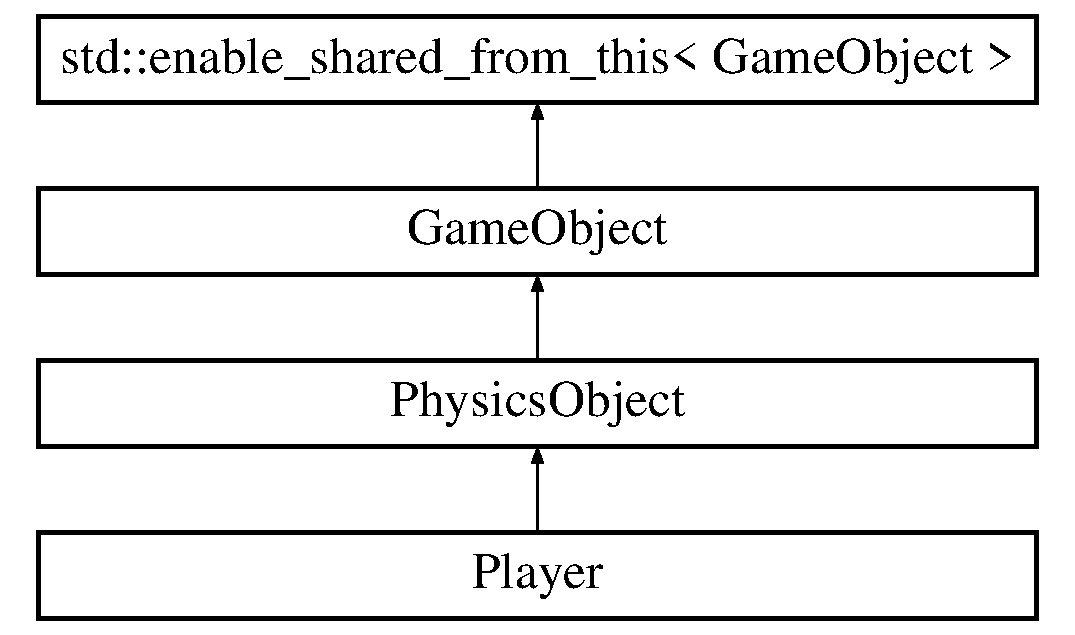
\includegraphics[height=4.000000cm]{d8/d53/class_player}
\end{center}
\end{figure}
\subsection*{Public Member Functions}
\begin{DoxyCompactItemize}
\item 
\mbox{\Hypertarget{class_player_affe0cc3cb714f6deb4e62f0c0d3f1fd8}\label{class_player_affe0cc3cb714f6deb4e62f0c0d3f1fd8}} 
\hyperlink{class_player_affe0cc3cb714f6deb4e62f0c0d3f1fd8}{Player} ()
\begin{DoxyCompactList}\small\item\em Redundant constructors need to be reworked. \end{DoxyCompactList}\item 
\hyperlink{class_player_afb985ed4c767e1ad824655b9f5f9d597}{Player} (\hyperlink{class_vector2_d}{Vector2D}$<$ double $>$ \&start\+Position, \hyperlink{class_character}{Character} player\+Stats)
\begin{DoxyCompactList}\small\item\em \hyperlink{class_player}{Player} constructor needs to be reworked too much database implementation is used. \end{DoxyCompactList}\item 
\mbox{\Hypertarget{class_player_a066cb6500937804121fd4ceb15595b3f}\label{class_player_a066cb6500937804121fd4ceb15595b3f}} 
{\bfseries Player} (\hyperlink{class_vector2_d}{Vector2D}$<$ double $>$ \&start\+Position, \hyperlink{class_character}{Character} player\+Stats, std\+::shared\+\_\+ptr$<$ \hyperlink{class_graphic_object}{Graphic\+Object} $>$ bullet\+Graphic)
\item 
\mbox{\Hypertarget{class_player_ad5023c3701c11222e09906b41c604135}\label{class_player_ad5023c3701c11222e09906b41c604135}} 
virtual \hyperlink{class_player}{Player} $\ast$ \hyperlink{class_player_ad5023c3701c11222e09906b41c604135}{Clone} () override
\begin{DoxyCompactList}\small\item\em Clone still in development. \end{DoxyCompactList}\item 
\mbox{\Hypertarget{class_player_a5e17be3418fa0ac0192c05efaf3dc8bd}\label{class_player_a5e17be3418fa0ac0192c05efaf3dc8bd}} 
void \hyperlink{class_player_a5e17be3418fa0ac0192c05efaf3dc8bd}{Update} () override
\begin{DoxyCompactList}\small\item\em could aslo be used as a friendship with scene \end{DoxyCompactList}\item 
virtual void \hyperlink{class_player_a965e7e8baf9b270e1b22784b890bc74d}{collision\+Action} (Game\+Object\+Type object\+Type) override
\item 
\mbox{\Hypertarget{class_player_a0bee9292374b568f74c2f9240fba0d36}\label{class_player_a0bee9292374b568f74c2f9240fba0d36}} 
const std\+::shared\+\_\+ptr$<$ \hyperlink{class_graphic_object}{Graphic\+Object} $>$ {\bfseries get\+Graphic\+Object} () override
\end{DoxyCompactItemize}
\subsection*{Additional Inherited Members}


\subsection{Detailed Description}
\hyperlink{class_character}{Character} rework required here as well. 

\subsection{Constructor \& Destructor Documentation}
\mbox{\Hypertarget{class_player_afb985ed4c767e1ad824655b9f5f9d597}\label{class_player_afb985ed4c767e1ad824655b9f5f9d597}} 
\index{Player@{Player}!Player@{Player}}
\index{Player@{Player}!Player@{Player}}
\subsubsection{\texorpdfstring{Player()}{Player()}}
{\footnotesize\ttfamily Player\+::\+Player (\begin{DoxyParamCaption}\item[{\hyperlink{class_vector2_d}{Vector2D}$<$ double $>$ \&}]{start\+Position,  }\item[{\hyperlink{class_character}{Character}}]{player\+Stats }\end{DoxyParamCaption})}



\hyperlink{class_player}{Player} constructor needs to be reworked too much database implementation is used. 

Needs to be stored in a database 

\subsection{Member Function Documentation}
\mbox{\Hypertarget{class_player_a965e7e8baf9b270e1b22784b890bc74d}\label{class_player_a965e7e8baf9b270e1b22784b890bc74d}} 
\index{Player@{Player}!collision\+Action@{collision\+Action}}
\index{collision\+Action@{collision\+Action}!Player@{Player}}
\subsubsection{\texorpdfstring{collision\+Action()}{collisionAction()}}
{\footnotesize\ttfamily void Player\+::collision\+Action (\begin{DoxyParamCaption}\item[{Game\+Object\+Type}]{object\+Type }\end{DoxyParamCaption})\hspace{0.3cm}{\ttfamily [override]}, {\ttfamily [virtual]}}

Magic Number needs to be removed (can be replaced by an enumerator class or static variable) 

Implements \hyperlink{class_physics_object}{Physics\+Object}.



The documentation for this class was generated from the following files\+:\begin{DoxyCompactItemize}
\item 
D\+:/\+Users/\+Tim-\/\+P\+C/\+Documents/\+Software\+\_\+\+I\+I/\+Project/\+Project\+Files/game-\/source-\/code/\+Front\+End\+Systems/Player.\+h\item 
D\+:/\+Users/\+Tim-\/\+P\+C/\+Documents/\+Software\+\_\+\+I\+I/\+Project/\+Project\+Files/game-\/source-\/code/\+Front\+End\+Systems/Player.\+cpp\end{DoxyCompactItemize}

\hypertarget{class_player_factory}{}\section{Player\+Factory Class Reference}
\label{class_player_factory}\index{Player\+Factory@{Player\+Factory}}


Derived class from the \hyperlink{class_game_object_factory}{Game\+Object\+Factory} interface used to construct the player object.  




{\ttfamily \#include $<$Player\+Factory.\+h$>$}

Inheritance diagram for Player\+Factory\+:\begin{figure}[H]
\begin{center}
\leavevmode
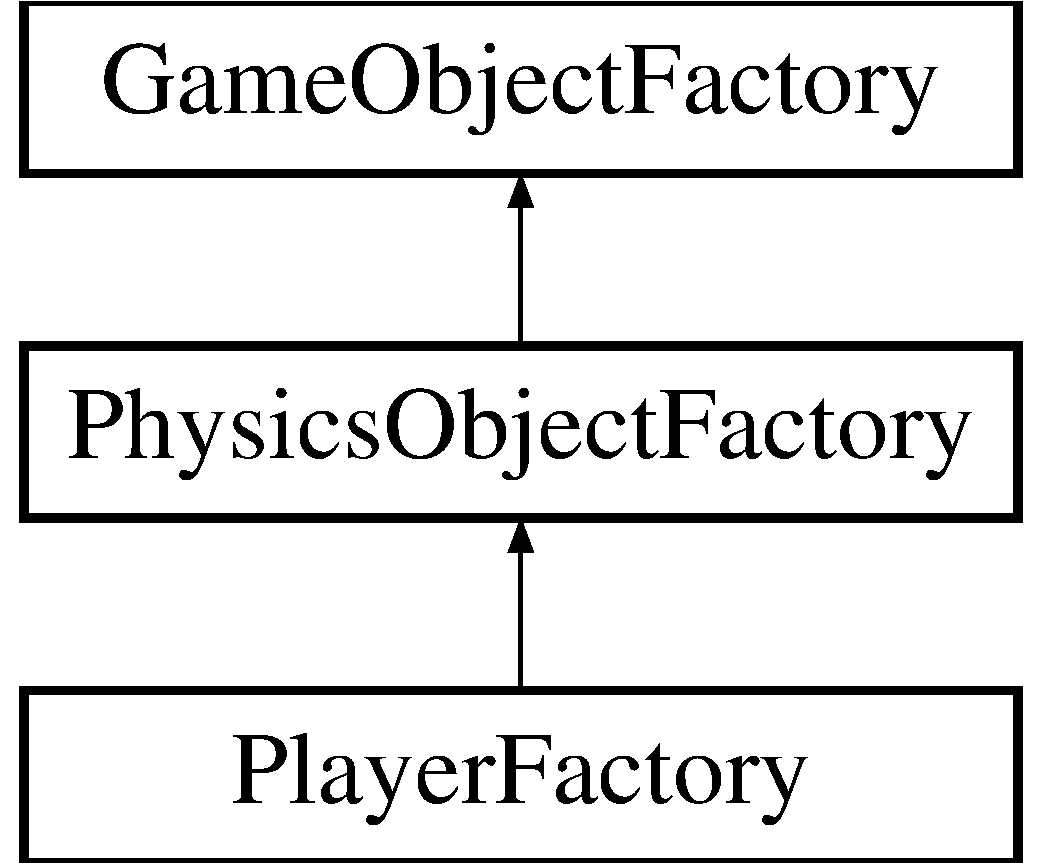
\includegraphics[height=3.000000cm]{df/dda/class_player_factory}
\end{center}
\end{figure}
\subsection*{Public Member Functions}
\begin{DoxyCompactItemize}
\item 
virtual std\+::shared\+\_\+ptr$<$ \hyperlink{class_game_object}{Game\+Object} $>$ \hyperlink{class_player_factory_ab92534e7d2d6887ecf9e4ed8131a8112}{get\+Game\+Object} (const std\+::shared\+\_\+ptr$<$ \hyperlink{class_database_interface}{Database\+Interface} $>$ \&database) override
\begin{DoxyCompactList}\small\item\em Constructs the player object. \end{DoxyCompactList}\item 
virtual \hyperlink{struct_game_object_data}{Game\+Object\+Data} \hyperlink{class_player_factory_aca4e809430541d77acd4c588c4381715}{get\+Object\+Data} (const std\+::shared\+\_\+ptr$<$ \hyperlink{class_database_interface}{Database\+Interface} $>$ \&database) override
\begin{DoxyCompactList}\small\item\em used to obtain the specific \hyperlink{struct_game_object_data}{Game\+Object\+Data} defined for the current factory \end{DoxyCompactList}\end{DoxyCompactItemize}


\subsection{Detailed Description}
Derived class from the \hyperlink{class_game_object_factory}{Game\+Object\+Factory} interface used to construct the player object. 

\subsection{Member Function Documentation}
\mbox{\Hypertarget{class_player_factory_ab92534e7d2d6887ecf9e4ed8131a8112}\label{class_player_factory_ab92534e7d2d6887ecf9e4ed8131a8112}} 
\index{Player\+Factory@{Player\+Factory}!get\+Game\+Object@{get\+Game\+Object}}
\index{get\+Game\+Object@{get\+Game\+Object}!Player\+Factory@{Player\+Factory}}
\subsubsection{\texorpdfstring{get\+Game\+Object()}{getGameObject()}}
{\footnotesize\ttfamily std\+::shared\+\_\+ptr$<$ \hyperlink{class_game_object}{Game\+Object} $>$ Player\+Factory\+::get\+Game\+Object (\begin{DoxyParamCaption}\item[{const std\+::shared\+\_\+ptr$<$ \hyperlink{class_database_interface}{Database\+Interface} $>$ \&}]{database }\end{DoxyParamCaption})\hspace{0.3cm}{\ttfamily [override]}, {\ttfamily [virtual]}}



Constructs the player object. 

\begin{DoxyReturn}{Returns}
Returns the construted player object 
\end{DoxyReturn}


Reimplemented from \hyperlink{class_physics_object_factory_a2644107d0c455c3307559cd824a7c9a8}{Physics\+Object\+Factory}.

\mbox{\Hypertarget{class_player_factory_aca4e809430541d77acd4c588c4381715}\label{class_player_factory_aca4e809430541d77acd4c588c4381715}} 
\index{Player\+Factory@{Player\+Factory}!get\+Object\+Data@{get\+Object\+Data}}
\index{get\+Object\+Data@{get\+Object\+Data}!Player\+Factory@{Player\+Factory}}
\subsubsection{\texorpdfstring{get\+Object\+Data()}{getObjectData()}}
{\footnotesize\ttfamily \hyperlink{struct_game_object_data}{Game\+Object\+Data} Player\+Factory\+::get\+Object\+Data (\begin{DoxyParamCaption}\item[{const std\+::shared\+\_\+ptr$<$ \hyperlink{class_database_interface}{Database\+Interface} $>$ \&}]{database }\end{DoxyParamCaption})\hspace{0.3cm}{\ttfamily [override]}, {\ttfamily [virtual]}}



used to obtain the specific \hyperlink{struct_game_object_data}{Game\+Object\+Data} defined for the current factory 


\begin{DoxyParams}{Parameters}
{\em database} & The specific \hyperlink{class_database_interface}{Database\+Interface} that contains the information about the Game\+Objects \\
\hline
\end{DoxyParams}
\begin{DoxyReturn}{Returns}
The \hyperlink{struct_game_object_data}{Game\+Object\+Data} required for the construction of the object 
\end{DoxyReturn}


Implements \hyperlink{class_physics_object_factory_aa59f52d3adc1fac676f4a8a3c2de9ba9}{Physics\+Object\+Factory}.



The documentation for this class was generated from the following files\+:\begin{DoxyCompactItemize}
\item 
D\+:/\+Users/\+Tim-\/\+P\+C/\+Documents/\+Software\+\_\+\+I\+I/\+Project/\+Project\+Files/game-\/source-\/code/\+Back\+End\+Systems/Player\+Factory.\+h\item 
D\+:/\+Users/\+Tim-\/\+P\+C/\+Documents/\+Software\+\_\+\+I\+I/\+Project/\+Project\+Files/game-\/source-\/code/\+Back\+End\+Systems/Player\+Factory.\+cpp\end{DoxyCompactItemize}

\hypertarget{class_player_move}{}\section{Player\+Move Class Reference}
\label{class_player_move}\index{Player\+Move@{Player\+Move}}


\hyperlink{class_player_move}{Player\+Move} is responsible for determining how the \hyperlink{class_player}{Player} Object moves.  




{\ttfamily \#include $<$Player\+Move.\+h$>$}

Inheritance diagram for Player\+Move\+:\begin{figure}[H]
\begin{center}
\leavevmode
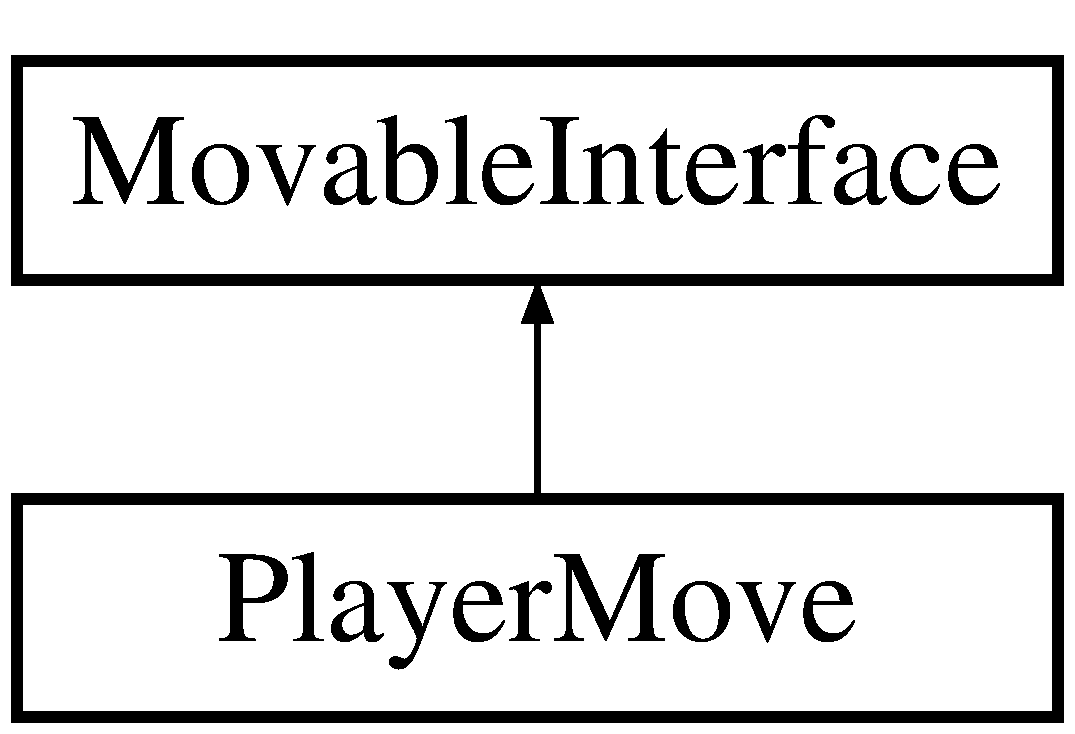
\includegraphics[height=2.000000cm]{d8/d6d/class_player_move}
\end{center}
\end{figure}
\subsection*{Public Member Functions}
\begin{DoxyCompactItemize}
\item 
\hyperlink{class_player_move_afac691eb4cb3f0fbbf1876b5991e3a80}{Player\+Move} (double move\+Speed)
\begin{DoxyCompactList}\small\item\em Constructs the \hyperlink{class_player_move}{Player\+Move} object with a desired speed. \end{DoxyCompactList}\item 
virtual void \hyperlink{class_player_move_a1c39885d4126c63441250eae23ac718a}{Move} (\hyperlink{class_vector2_d}{Vector2D} \&current\+Position) override
\begin{DoxyCompactList}\small\item\em Moves the provided \hyperlink{class_vector2_d}{Vector2D} in a circle based on input from the user. \end{DoxyCompactList}\end{DoxyCompactItemize}
\subsection*{Private Member Functions}
\begin{DoxyCompactItemize}
\item 
int \hyperlink{class_player_move_a8118719df3dd369686b41a0ec77cd8e0}{determine\+Move\+Direction} ()
\begin{DoxyCompactList}\small\item\em determines the direction of movement based off of the user input \end{DoxyCompactList}\end{DoxyCompactItemize}
\subsection*{Additional Inherited Members}


\subsection{Detailed Description}
\hyperlink{class_player_move}{Player\+Move} is responsible for determining how the \hyperlink{class_player}{Player} Object moves. 

\hyperlink{class_player_move}{Player\+Move} checks for an input from the user then changes the position 

\subsection{Constructor \& Destructor Documentation}
\mbox{\Hypertarget{class_player_move_afac691eb4cb3f0fbbf1876b5991e3a80}\label{class_player_move_afac691eb4cb3f0fbbf1876b5991e3a80}} 
\index{Player\+Move@{Player\+Move}!Player\+Move@{Player\+Move}}
\index{Player\+Move@{Player\+Move}!Player\+Move@{Player\+Move}}
\subsubsection{\texorpdfstring{Player\+Move()}{PlayerMove()}}
{\footnotesize\ttfamily Player\+Move\+::\+Player\+Move (\begin{DoxyParamCaption}\item[{double}]{move\+Speed }\end{DoxyParamCaption})}



Constructs the \hyperlink{class_player_move}{Player\+Move} object with a desired speed. 


\begin{DoxyParams}{Parameters}
{\em move\+Speed} & The desired movement speed for the player \\
\hline
\end{DoxyParams}


\subsection{Member Function Documentation}
\mbox{\Hypertarget{class_player_move_a8118719df3dd369686b41a0ec77cd8e0}\label{class_player_move_a8118719df3dd369686b41a0ec77cd8e0}} 
\index{Player\+Move@{Player\+Move}!determine\+Move\+Direction@{determine\+Move\+Direction}}
\index{determine\+Move\+Direction@{determine\+Move\+Direction}!Player\+Move@{Player\+Move}}
\subsubsection{\texorpdfstring{determine\+Move\+Direction()}{determineMoveDirection()}}
{\footnotesize\ttfamily int Player\+Move\+::determine\+Move\+Direction (\begin{DoxyParamCaption}{ }\end{DoxyParamCaption})\hspace{0.3cm}{\ttfamily [private]}}



determines the direction of movement based off of the user input 

\begin{DoxyReturn}{Returns}
returns an integer of -\/1,0,1 depending on the users input 
\end{DoxyReturn}
\mbox{\Hypertarget{class_player_move_a1c39885d4126c63441250eae23ac718a}\label{class_player_move_a1c39885d4126c63441250eae23ac718a}} 
\index{Player\+Move@{Player\+Move}!Move@{Move}}
\index{Move@{Move}!Player\+Move@{Player\+Move}}
\subsubsection{\texorpdfstring{Move()}{Move()}}
{\footnotesize\ttfamily void Player\+Move\+::\+Move (\begin{DoxyParamCaption}\item[{\hyperlink{class_vector2_d}{Vector2D} \&}]{current\+Position }\end{DoxyParamCaption})\hspace{0.3cm}{\ttfamily [override]}, {\ttfamily [virtual]}}



Moves the provided \hyperlink{class_vector2_d}{Vector2D} in a circle based on input from the user. 


\begin{DoxyParams}{Parameters}
{\em current\+Position} & \\
\hline
\end{DoxyParams}


Implements \hyperlink{class_movable_interface_a899cc1c78eacbee13b906c6770e7f025}{Movable\+Interface}.



The documentation for this class was generated from the following files\+:\begin{DoxyCompactItemize}
\item 
C\+:/\+Users/\+Tim/\+Documents/\+Software\+Dev/\+Software\+Project/\+Project\+Files/game-\/source-\/code/\+Front\+End\+Systems/Player\+Move.\+h\item 
C\+:/\+Users/\+Tim/\+Documents/\+Software\+Dev/\+Software\+Project/\+Project\+Files/game-\/source-\/code/\+Front\+End\+Systems/Player\+Move.\+cpp\end{DoxyCompactItemize}

\hypertarget{class_player_projectile}{}\section{Player\+Projectile Class Reference}
\label{class_player_projectile}\index{Player\+Projectile@{Player\+Projectile}}


Used to represent the \hyperlink{class_player_projectile}{Player\+Projectile} within the game.  




{\ttfamily \#include $<$Player\+Projectile.\+h$>$}

Inheritance diagram for Player\+Projectile\+:\begin{figure}[H]
\begin{center}
\leavevmode
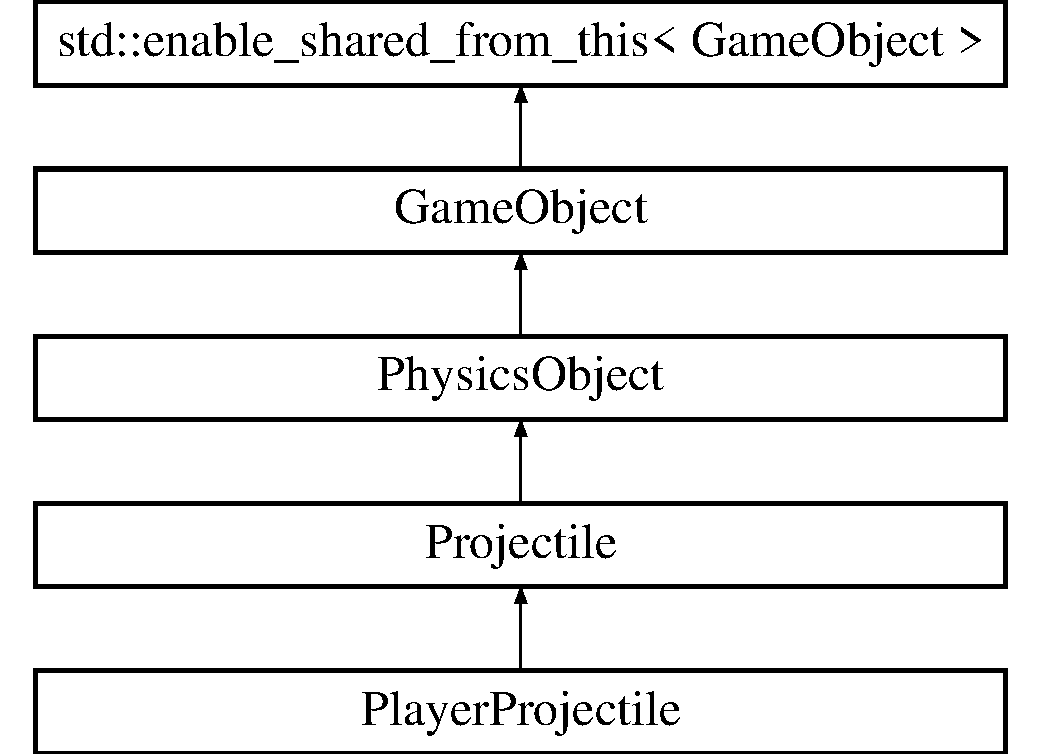
\includegraphics[height=5.000000cm]{d5/df1/class_player_projectile}
\end{center}
\end{figure}
\subsection*{Public Member Functions}
\begin{DoxyCompactItemize}
\item 
\hyperlink{class_player_projectile_a81e6c16b0d8ce85bad2e8e4b30d2607e}{Player\+Projectile} (const \hyperlink{class_physics_object}{Physics\+Object} \&physics\+Object, const std\+::shared\+\_\+ptr$<$ \hyperlink{class_movable_interface}{Movable\+Interface} $>$ \&move, const \hyperlink{class_boundary}{Boundary} \&destroy\+Bounds)
\begin{DoxyCompactList}\small\item\em Constructs the \hyperlink{class_player_projectile}{Player\+Projectile} Object. \end{DoxyCompactList}\item 
\mbox{\Hypertarget{class_player_projectile_a05a6c103f9fbae57bfc811e477ab7b5b}\label{class_player_projectile_a05a6c103f9fbae57bfc811e477ab7b5b}} 
virtual void \hyperlink{class_player_projectile_a05a6c103f9fbae57bfc811e477ab7b5b}{Destroy\+Self} () override
\begin{DoxyCompactList}\small\item\em Destroyed itself when the object is close to the centre of the screen (inside the \hyperlink{class_boundary}{Boundary} defined) \end{DoxyCompactList}\item 
virtual void \hyperlink{class_player_projectile_a22fcdd7296d95b97ae60b4d20d8a57bd}{collision\+Action} (const Game\+Object\+Type \&object\+Type) override
\begin{DoxyCompactList}\small\item\em Destroys itself when the object collides with the various types of enemy objects. \end{DoxyCompactList}\end{DoxyCompactItemize}
\subsection*{Additional Inherited Members}


\subsection{Detailed Description}
Used to represent the \hyperlink{class_player_projectile}{Player\+Projectile} within the game. 

The template design pattern is used to create the \hyperlink{class_player_projectile}{Player\+Projectile} from the base \hyperlink{class_projectile}{Projectile} object so that only the most necessary functions are overriden to vary the \hyperlink{class_player_projectile}{Player\+Projectile} and the \hyperlink{class_enemy_projectile}{Enemy\+Projectile} 

\subsection{Constructor \& Destructor Documentation}
\mbox{\Hypertarget{class_player_projectile_a81e6c16b0d8ce85bad2e8e4b30d2607e}\label{class_player_projectile_a81e6c16b0d8ce85bad2e8e4b30d2607e}} 
\index{Player\+Projectile@{Player\+Projectile}!Player\+Projectile@{Player\+Projectile}}
\index{Player\+Projectile@{Player\+Projectile}!Player\+Projectile@{Player\+Projectile}}
\subsubsection{\texorpdfstring{Player\+Projectile()}{PlayerProjectile()}}
{\footnotesize\ttfamily Player\+Projectile\+::\+Player\+Projectile (\begin{DoxyParamCaption}\item[{const \hyperlink{class_physics_object}{Physics\+Object} \&}]{physics\+Object,  }\item[{const std\+::shared\+\_\+ptr$<$ \hyperlink{class_movable_interface}{Movable\+Interface} $>$ \&}]{move,  }\item[{const \hyperlink{class_boundary}{Boundary} \&}]{destroy\+Bounds }\end{DoxyParamCaption})}



Constructs the \hyperlink{class_player_projectile}{Player\+Projectile} Object. 


\begin{DoxyParams}{Parameters}
{\em physics\+Object} & Base \hyperlink{class_physics_object}{Physics\+Object} members are copied \\
\hline
{\em move} & The \hyperlink{class_movable_interface}{Movable\+Interface} that defined the movement style for the projectile \\
\hline
{\em destroy\+Bounds} & The region in which the Porjectile is destroyed when it is inside of it \\
\hline
\end{DoxyParams}


\subsection{Member Function Documentation}
\mbox{\Hypertarget{class_player_projectile_a22fcdd7296d95b97ae60b4d20d8a57bd}\label{class_player_projectile_a22fcdd7296d95b97ae60b4d20d8a57bd}} 
\index{Player\+Projectile@{Player\+Projectile}!collision\+Action@{collision\+Action}}
\index{collision\+Action@{collision\+Action}!Player\+Projectile@{Player\+Projectile}}
\subsubsection{\texorpdfstring{collision\+Action()}{collisionAction()}}
{\footnotesize\ttfamily void Player\+Projectile\+::collision\+Action (\begin{DoxyParamCaption}\item[{const Game\+Object\+Type \&}]{object\+Type }\end{DoxyParamCaption})\hspace{0.3cm}{\ttfamily [override]}, {\ttfamily [virtual]}}



Destroys itself when the object collides with the various types of enemy objects. 


\begin{DoxyParams}{Parameters}
{\em object\+Type} & The Game\+Object\+Type representing the type of object that was collided with \\
\hline
\end{DoxyParams}


Reimplemented from \hyperlink{class_physics_object_a16163f4e5bf781b3814d024c9f44a276}{Physics\+Object}.



The documentation for this class was generated from the following files\+:\begin{DoxyCompactItemize}
\item 
C\+:/\+Users/\+Tim/\+Documents/\+Software\+Dev/\+Software\+Project/\+Project\+Files/game-\/source-\/code/\+Front\+End\+Systems/Player\+Projectile.\+h\item 
C\+:/\+Users/\+Tim/\+Documents/\+Software\+Dev/\+Software\+Project/\+Project\+Files/game-\/source-\/code/\+Front\+End\+Systems/Player\+Projectile.\+cpp\end{DoxyCompactItemize}

\hypertarget{class_player_projectile_factory}{}\section{Player\+Projectile\+Factory Class Reference}
\label{class_player_projectile_factory}\index{Player\+Projectile\+Factory@{Player\+Projectile\+Factory}}


\hyperlink{class_player_projectile_factory}{Player\+Projectile\+Factory} is responsible for the construction of any \hyperlink{class_player_projectile}{Player\+Projectile} objects.  




{\ttfamily \#include $<$Player\+Projectile\+Factory.\+h$>$}

Inheritance diagram for Player\+Projectile\+Factory\+:\begin{figure}[H]
\begin{center}
\leavevmode
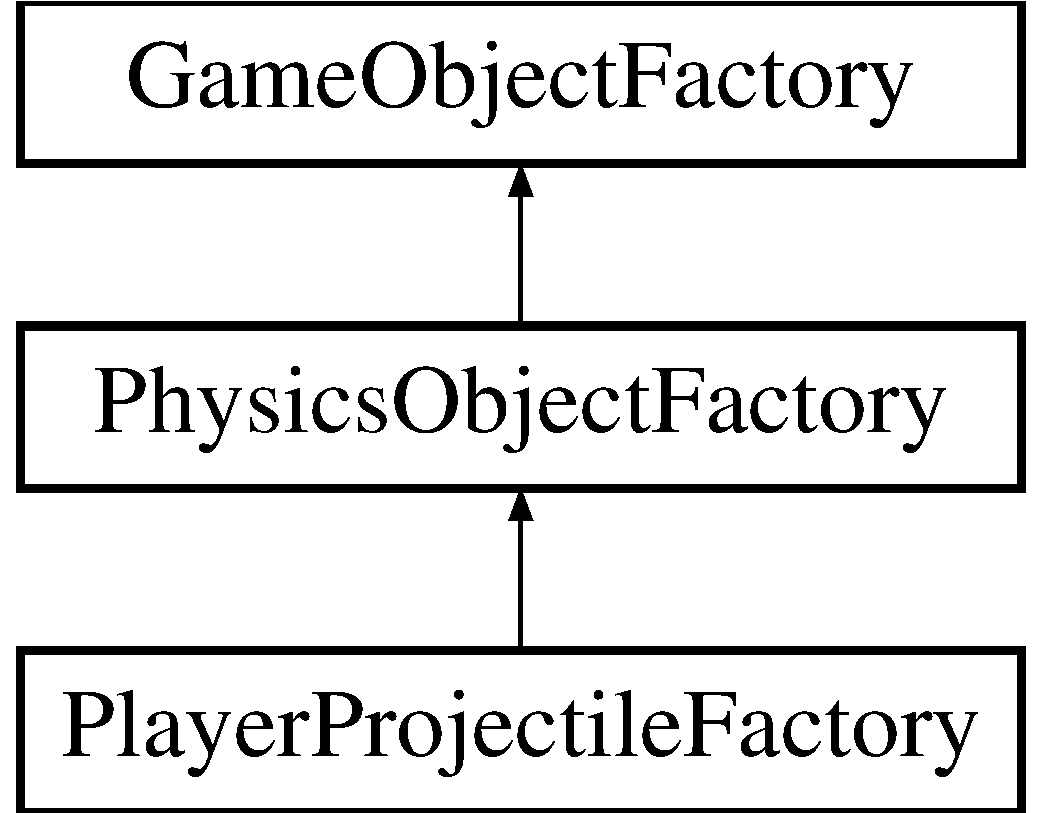
\includegraphics[height=3.000000cm]{d7/dd5/class_player_projectile_factory}
\end{center}
\end{figure}
\subsection*{Public Member Functions}
\begin{DoxyCompactItemize}
\item 
virtual std\+::shared\+\_\+ptr$<$ \hyperlink{class_game_object}{Game\+Object} $>$ \hyperlink{class_player_projectile_factory_a804a9f591ce6f0a7fb04f35ff685ff57}{get\+Game\+Object} (const std\+::shared\+\_\+ptr$<$ \hyperlink{class_database_interface}{Database\+Interface} $>$ \&database) override
\begin{DoxyCompactList}\small\item\em Function call used to create an \hyperlink{class_player_projectile}{Player\+Projectile} Object. \end{DoxyCompactList}\item 
virtual \hyperlink{struct_game_object_data}{Game\+Object\+Data} \hyperlink{class_player_projectile_factory_a702ae964c9dc653140fad4e17f38f60a}{get\+Object\+Data} (const std\+::shared\+\_\+ptr$<$ \hyperlink{class_database_interface}{Database\+Interface} $>$ \&database) override
\begin{DoxyCompactList}\small\item\em used to obtain the specific \hyperlink{struct_game_object_data}{Game\+Object\+Data} defined for the current factory \end{DoxyCompactList}\end{DoxyCompactItemize}


\subsection{Detailed Description}
\hyperlink{class_player_projectile_factory}{Player\+Projectile\+Factory} is responsible for the construction of any \hyperlink{class_player_projectile}{Player\+Projectile} objects. 

\subsection{Member Function Documentation}
\mbox{\Hypertarget{class_player_projectile_factory_a804a9f591ce6f0a7fb04f35ff685ff57}\label{class_player_projectile_factory_a804a9f591ce6f0a7fb04f35ff685ff57}} 
\index{Player\+Projectile\+Factory@{Player\+Projectile\+Factory}!get\+Game\+Object@{get\+Game\+Object}}
\index{get\+Game\+Object@{get\+Game\+Object}!Player\+Projectile\+Factory@{Player\+Projectile\+Factory}}
\subsubsection{\texorpdfstring{get\+Game\+Object()}{getGameObject()}}
{\footnotesize\ttfamily std\+::shared\+\_\+ptr$<$ \hyperlink{class_game_object}{Game\+Object} $>$ Player\+Projectile\+Factory\+::get\+Game\+Object (\begin{DoxyParamCaption}\item[{const std\+::shared\+\_\+ptr$<$ \hyperlink{class_database_interface}{Database\+Interface} $>$ \&}]{database }\end{DoxyParamCaption})\hspace{0.3cm}{\ttfamily [override]}, {\ttfamily [virtual]}}



Function call used to create an \hyperlink{class_player_projectile}{Player\+Projectile} Object. 

\begin{DoxyReturn}{Returns}
Returns an An \hyperlink{class_player_projectile}{Player\+Projectile} Object with the specific characteristics for this game 
\end{DoxyReturn}


Reimplemented from \hyperlink{class_physics_object_factory_a2644107d0c455c3307559cd824a7c9a8}{Physics\+Object\+Factory}.

\mbox{\Hypertarget{class_player_projectile_factory_a702ae964c9dc653140fad4e17f38f60a}\label{class_player_projectile_factory_a702ae964c9dc653140fad4e17f38f60a}} 
\index{Player\+Projectile\+Factory@{Player\+Projectile\+Factory}!get\+Object\+Data@{get\+Object\+Data}}
\index{get\+Object\+Data@{get\+Object\+Data}!Player\+Projectile\+Factory@{Player\+Projectile\+Factory}}
\subsubsection{\texorpdfstring{get\+Object\+Data()}{getObjectData()}}
{\footnotesize\ttfamily \hyperlink{struct_game_object_data}{Game\+Object\+Data} Player\+Projectile\+Factory\+::get\+Object\+Data (\begin{DoxyParamCaption}\item[{const std\+::shared\+\_\+ptr$<$ \hyperlink{class_database_interface}{Database\+Interface} $>$ \&}]{database }\end{DoxyParamCaption})\hspace{0.3cm}{\ttfamily [override]}, {\ttfamily [virtual]}}



used to obtain the specific \hyperlink{struct_game_object_data}{Game\+Object\+Data} defined for the current factory 


\begin{DoxyParams}{Parameters}
{\em database} & The specific \hyperlink{class_database_interface}{Database\+Interface} that contains the information about the Game\+Objects \\
\hline
\end{DoxyParams}
\begin{DoxyReturn}{Returns}
The \hyperlink{struct_game_object_data}{Game\+Object\+Data} required for the construction of the object 
\end{DoxyReturn}


Implements \hyperlink{class_physics_object_factory_aa59f52d3adc1fac676f4a8a3c2de9ba9}{Physics\+Object\+Factory}.



The documentation for this class was generated from the following files\+:\begin{DoxyCompactItemize}
\item 
C\+:/\+Users/\+Tim/\+Documents/\+Software\+Dev/\+Software\+Project/\+Project\+Files/game-\/source-\/code/\+Back\+End\+Systems/Player\+Projectile\+Factory.\+h\item 
C\+:/\+Users/\+Tim/\+Documents/\+Software\+Dev/\+Software\+Project/\+Project\+Files/game-\/source-\/code/\+Back\+End\+Systems/Player\+Projectile\+Factory.\+cpp\end{DoxyCompactItemize}

\hypertarget{class_projectile}{}\section{Projectile Class Reference}
\label{class_projectile}\index{Projectile@{Projectile}}


{\ttfamily \#include $<$Projectile.\+h$>$}

Inheritance diagram for Projectile\+:\begin{figure}[H]
\begin{center}
\leavevmode
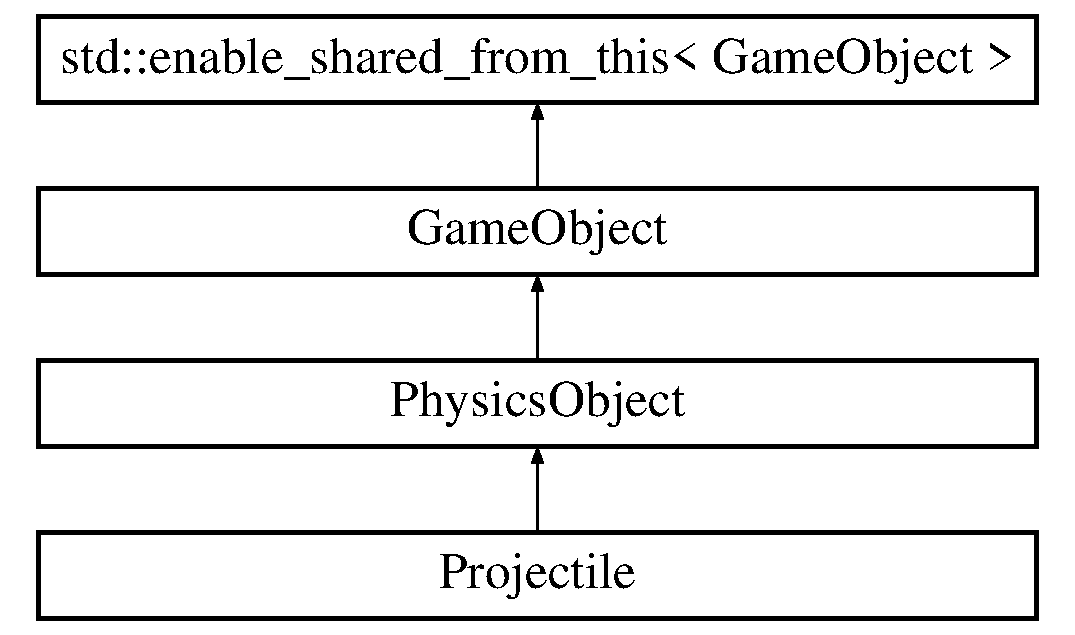
\includegraphics[height=4.000000cm]{db/dbe/class_projectile}
\end{center}
\end{figure}
\subsection*{Public Member Functions}
\begin{DoxyCompactItemize}
\item 
\mbox{\Hypertarget{class_projectile_ac536ed2aad56af866a2078b9a85aa16d}\label{class_projectile_ac536ed2aad56af866a2078b9a85aa16d}} 
\hyperlink{class_projectile_ac536ed2aad56af866a2078b9a85aa16d}{Projectile} ()
\begin{DoxyCompactList}\small\item\em Constructors need to be redesigned. \end{DoxyCompactList}\item 
\mbox{\Hypertarget{class_projectile_a45f5e2eb6db9f673670e9de0aa9b9bab}\label{class_projectile_a45f5e2eb6db9f673670e9de0aa9b9bab}} 
{\bfseries Projectile} (Game\+Object\+Type projectile\+Type)
\item 
\mbox{\Hypertarget{class_projectile_a6d13e20ed5be714a7efd4be89791ea94}\label{class_projectile_a6d13e20ed5be714a7efd4be89791ea94}} 
\hyperlink{class_projectile_a6d13e20ed5be714a7efd4be89791ea94}{Projectile} (std\+::shared\+\_\+ptr$<$ \hyperlink{class_graphic_object}{Graphic\+Object} $>$ bullet\+Graphic, Game\+Object\+Type projectile\+Type, \hyperlink{structxy_vector}{xy\+Vector} scale)
\begin{DoxyCompactList}\small\item\em Constructor Needs a Database Dependency. \end{DoxyCompactList}\item 
\mbox{\Hypertarget{class_projectile_a60b9863678645f9605bf938ef6df7938}\label{class_projectile_a60b9863678645f9605bf938ef6df7938}} 
{\bfseries Projectile} (const \hyperlink{class_projectile}{Projectile} \&copy\+Projectile)
\item 
\mbox{\Hypertarget{class_projectile_ad057a8aeadb0064aacd0f93b2d6de158}\label{class_projectile_ad057a8aeadb0064aacd0f93b2d6de158}} 
virtual void \hyperlink{class_projectile_ad057a8aeadb0064aacd0f93b2d6de158}{Update} () override
\begin{DoxyCompactList}\small\item\em could aslo be used as a friendship with scene \end{DoxyCompactList}\item 
\mbox{\Hypertarget{class_projectile_aedb2c1ee7933578088e4d2a60d9c0f5c}\label{class_projectile_aedb2c1ee7933578088e4d2a60d9c0f5c}} 
void {\bfseries Initialise} (\hyperlink{class_vector2_d}{Vector2D}$<$ double $>$ starting\+Pos, \hyperlink{class_vector2_d}{Vector2D}$<$ double $>$ direction, double move\+Speed)
\item 
\mbox{\Hypertarget{class_projectile_a8dae5b6cc0293fc6c85797fcf2019492}\label{class_projectile_a8dae5b6cc0293fc6c85797fcf2019492}} 
virtual void \hyperlink{class_projectile_a8dae5b6cc0293fc6c85797fcf2019492}{collision\+Action} (Game\+Object\+Type object\+Type) override
\begin{DoxyCompactList}\small\item\em polymorphism will reduce this complexity \end{DoxyCompactList}\item 
\mbox{\Hypertarget{class_projectile_a639f52184c8b9720ca8c36371303332d}\label{class_projectile_a639f52184c8b9720ca8c36371303332d}} 
virtual const std\+::shared\+\_\+ptr$<$ \hyperlink{class_graphic_object}{Graphic\+Object} $>$ {\bfseries get\+Graphic\+Object} () override
\item 
\mbox{\Hypertarget{class_projectile_a39653a4aa80df0364e15854f0f5e389d}\label{class_projectile_a39653a4aa80df0364e15854f0f5e389d}} 
virtual \hyperlink{class_projectile}{Projectile} $\ast$ \hyperlink{class_projectile_a39653a4aa80df0364e15854f0f5e389d}{Clone} () override
\begin{DoxyCompactList}\small\item\em Clone Function Still in development. \end{DoxyCompactList}\item 
\mbox{\Hypertarget{class_projectile_add4d983566a326200ea1d7c74737e108}\label{class_projectile_add4d983566a326200ea1d7c74737e108}} 
\hyperlink{class_projectile_add4d983566a326200ea1d7c74737e108}{$\sim$\+Projectile} () override
\begin{DoxyCompactList}\small\item\em Needs the virtual tag. \end{DoxyCompactList}\end{DoxyCompactItemize}
\subsection*{Additional Inherited Members}


\subsection{Detailed Description}
Object needs to be converted into a polymorphic object, one for player and one for enemy with virtual destorys and boundaries corresponds to the type information in a better way 

The documentation for this class was generated from the following files\+:\begin{DoxyCompactItemize}
\item 
D\+:/\+Users/\+Tim-\/\+P\+C/\+Documents/\+Software\+\_\+\+I\+I/\+Project/\+Project\+Files/game-\/source-\/code/\+Front\+End\+Systems/Projectile.\+h\item 
D\+:/\+Users/\+Tim-\/\+P\+C/\+Documents/\+Software\+\_\+\+I\+I/\+Project/\+Project\+Files/game-\/source-\/code/\+Front\+End\+Systems/Projectile.\+cpp\end{DoxyCompactItemize}

\hypertarget{class_random_enemy_factory}{}\section{Random\+Enemy\+Factory Class Reference}
\label{class_random_enemy_factory}\index{Random\+Enemy\+Factory@{Random\+Enemy\+Factory}}


Used to construct a specific enemy at Random.  




{\ttfamily \#include $<$Random\+Enemy\+Factory.\+h$>$}

Inheritance diagram for Random\+Enemy\+Factory\+:\begin{figure}[H]
\begin{center}
\leavevmode
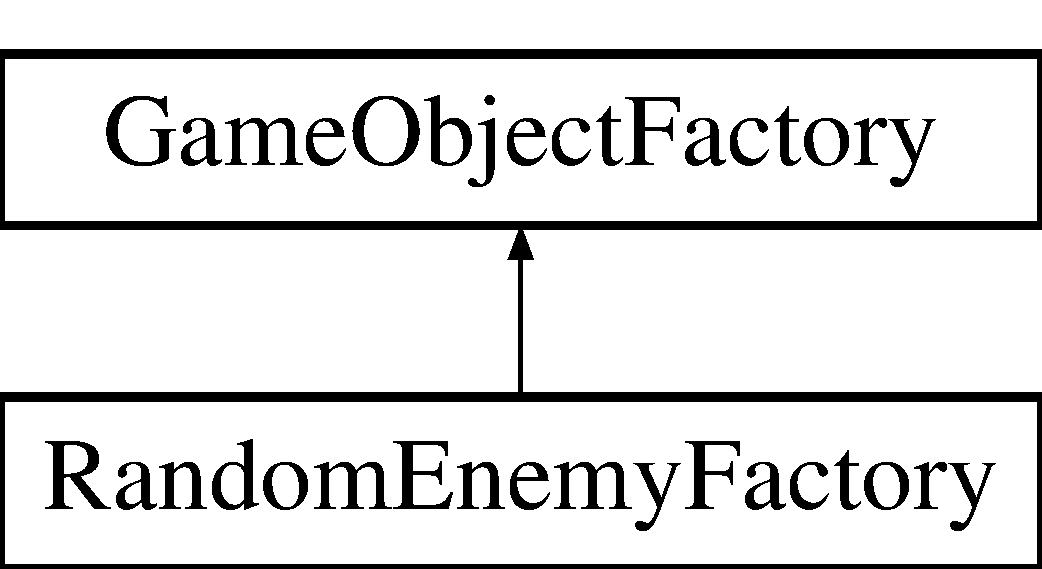
\includegraphics[height=2.000000cm]{df/def/class_random_enemy_factory}
\end{center}
\end{figure}
\subsection*{Public Member Functions}
\begin{DoxyCompactItemize}
\item 
virtual std\+::shared\+\_\+ptr$<$ \hyperlink{class_game_object}{Game\+Object} $>$ \hyperlink{class_random_enemy_factory_a5099fcf010a5cf2f53fd7c874a1925a9}{get\+Game\+Object} (const std\+::shared\+\_\+ptr$<$ \hyperlink{class_database_interface}{Database\+Interface} $>$ \&database) override
\begin{DoxyCompactList}\small\item\em Constructs a Random \hyperlink{class_enemy}{Enemy} by using the defined \hyperlink{class_enemy}{Enemy} Factories. \end{DoxyCompactList}\item 
\hyperlink{struct_game_object_data}{Game\+Object\+Data} \hyperlink{class_random_enemy_factory_a7c007b44a5e5e59fecc0b8cd2a6a9dc3}{get\+Object\+Data} (const std\+::shared\+\_\+ptr$<$ \hyperlink{class_database_interface}{Database\+Interface} $>$ \&database)
\begin{DoxyCompactList}\small\item\em used to obtain the specific \hyperlink{struct_game_object_data}{Game\+Object\+Data} defined for the current factory \end{DoxyCompactList}\end{DoxyCompactItemize}
\subsection*{Private Member Functions}
\begin{DoxyCompactItemize}
\item 
std\+::shared\+\_\+ptr$<$ \hyperlink{class_game_object_factory}{Game\+Object\+Factory} $>$ \hyperlink{class_random_enemy_factory_a8a9643918f3e727aac7e41c6187a9d9a}{get\+Random\+Factory} ()
\begin{DoxyCompactList}\small\item\em Creates an \hyperlink{class_enemy_factory}{Enemy\+Factory} at Random. \end{DoxyCompactList}\end{DoxyCompactItemize}
\subsection*{Private Attributes}
\begin{DoxyCompactItemize}
\item 
const unsigned int \hyperlink{class_random_enemy_factory_ac912e49add9d56e8b12d3881ce1cc656}{S\+P\+I\+R\+A\+L\+\_\+\+P\+E\+R\+C\+E\+N\+T\+A\+G\+E\+\_\+\+V\+A\+L\+UE} = 80
\item 
const unsigned int \hyperlink{class_random_enemy_factory_ad52b65e560c09a560d7be11c97997f5c}{L\+I\+N\+E\+A\+R\+\_\+\+P\+E\+R\+C\+E\+N\+T\+A\+G\+E\+\_\+\+V\+A\+L\+UE} = 30
\item 
const unsigned int \hyperlink{class_random_enemy_factory_a64c95136e3e30f504755037e3f804372}{P\+A\+R\+A\+B\+O\+L\+I\+C\+\_\+\+P\+E\+R\+C\+E\+N\+T\+A\+G\+E\+\_\+\+V\+A\+L\+UE} = 0
\item 
const unsigned int \hyperlink{class_random_enemy_factory_ac3e384acfa1fa3927d3a3643647072e9}{M\+A\+X\+\_\+\+P\+E\+R\+C\+E\+N\+T\+A\+GE} = 100
\end{DoxyCompactItemize}


\subsection{Detailed Description}
Used to construct a specific enemy at Random. 

\subsection{Member Function Documentation}
\mbox{\Hypertarget{class_random_enemy_factory_a5099fcf010a5cf2f53fd7c874a1925a9}\label{class_random_enemy_factory_a5099fcf010a5cf2f53fd7c874a1925a9}} 
\index{Random\+Enemy\+Factory@{Random\+Enemy\+Factory}!get\+Game\+Object@{get\+Game\+Object}}
\index{get\+Game\+Object@{get\+Game\+Object}!Random\+Enemy\+Factory@{Random\+Enemy\+Factory}}
\subsubsection{\texorpdfstring{get\+Game\+Object()}{getGameObject()}}
{\footnotesize\ttfamily std\+::shared\+\_\+ptr$<$ \hyperlink{class_game_object}{Game\+Object} $>$ Random\+Enemy\+Factory\+::get\+Game\+Object (\begin{DoxyParamCaption}\item[{const std\+::shared\+\_\+ptr$<$ \hyperlink{class_database_interface}{Database\+Interface} $>$ \&}]{database }\end{DoxyParamCaption})\hspace{0.3cm}{\ttfamily [override]}, {\ttfamily [virtual]}}



Constructs a Random \hyperlink{class_enemy}{Enemy} by using the defined \hyperlink{class_enemy}{Enemy} Factories. 


\begin{DoxyParams}{Parameters}
{\em database} & The \hyperlink{class_database_interface}{Database\+Interface} that contains the information about the various Game\+Objects \\
\hline
\end{DoxyParams}
\begin{DoxyReturn}{Returns}
Returns The Random \hyperlink{class_enemy}{Enemy} Constructed 
\end{DoxyReturn}


Reimplemented from \hyperlink{class_game_object_factory_a5b684a6e77fb82c041f1721eb07c553d}{Game\+Object\+Factory}.

\mbox{\Hypertarget{class_random_enemy_factory_a7c007b44a5e5e59fecc0b8cd2a6a9dc3}\label{class_random_enemy_factory_a7c007b44a5e5e59fecc0b8cd2a6a9dc3}} 
\index{Random\+Enemy\+Factory@{Random\+Enemy\+Factory}!get\+Object\+Data@{get\+Object\+Data}}
\index{get\+Object\+Data@{get\+Object\+Data}!Random\+Enemy\+Factory@{Random\+Enemy\+Factory}}
\subsubsection{\texorpdfstring{get\+Object\+Data()}{getObjectData()}}
{\footnotesize\ttfamily \hyperlink{struct_game_object_data}{Game\+Object\+Data} Random\+Enemy\+Factory\+::get\+Object\+Data (\begin{DoxyParamCaption}\item[{const std\+::shared\+\_\+ptr$<$ \hyperlink{class_database_interface}{Database\+Interface} $>$ \&}]{database }\end{DoxyParamCaption})\hspace{0.3cm}{\ttfamily [virtual]}}



used to obtain the specific \hyperlink{struct_game_object_data}{Game\+Object\+Data} defined for the current factory 


\begin{DoxyParams}{Parameters}
{\em database} & The specific \hyperlink{class_database_interface}{Database\+Interface} that contains the information about the Game\+Objects \\
\hline
\end{DoxyParams}
\begin{DoxyReturn}{Returns}
The \hyperlink{struct_game_object_data}{Game\+Object\+Data} required for the construction of the object 
\end{DoxyReturn}


Implements \hyperlink{class_game_object_factory_ae9358fbb3ef2d3b127320341760d3ff9}{Game\+Object\+Factory}.

\mbox{\Hypertarget{class_random_enemy_factory_a8a9643918f3e727aac7e41c6187a9d9a}\label{class_random_enemy_factory_a8a9643918f3e727aac7e41c6187a9d9a}} 
\index{Random\+Enemy\+Factory@{Random\+Enemy\+Factory}!get\+Random\+Factory@{get\+Random\+Factory}}
\index{get\+Random\+Factory@{get\+Random\+Factory}!Random\+Enemy\+Factory@{Random\+Enemy\+Factory}}
\subsubsection{\texorpdfstring{get\+Random\+Factory()}{getRandomFactory()}}
{\footnotesize\ttfamily std\+::shared\+\_\+ptr$<$ \hyperlink{class_game_object_factory}{Game\+Object\+Factory} $>$ Random\+Enemy\+Factory\+::get\+Random\+Factory (\begin{DoxyParamCaption}{ }\end{DoxyParamCaption})\hspace{0.3cm}{\ttfamily [private]}}



Creates an \hyperlink{class_enemy_factory}{Enemy\+Factory} at Random. 

\begin{DoxyReturn}{Returns}
Returns the constructed \hyperlink{class_enemy_factory}{Enemy\+Factory} 
\end{DoxyReturn}


\subsection{Member Data Documentation}
\mbox{\Hypertarget{class_random_enemy_factory_ad52b65e560c09a560d7be11c97997f5c}\label{class_random_enemy_factory_ad52b65e560c09a560d7be11c97997f5c}} 
\index{Random\+Enemy\+Factory@{Random\+Enemy\+Factory}!L\+I\+N\+E\+A\+R\+\_\+\+P\+E\+R\+C\+E\+N\+T\+A\+G\+E\+\_\+\+V\+A\+L\+UE@{L\+I\+N\+E\+A\+R\+\_\+\+P\+E\+R\+C\+E\+N\+T\+A\+G\+E\+\_\+\+V\+A\+L\+UE}}
\index{L\+I\+N\+E\+A\+R\+\_\+\+P\+E\+R\+C\+E\+N\+T\+A\+G\+E\+\_\+\+V\+A\+L\+UE@{L\+I\+N\+E\+A\+R\+\_\+\+P\+E\+R\+C\+E\+N\+T\+A\+G\+E\+\_\+\+V\+A\+L\+UE}!Random\+Enemy\+Factory@{Random\+Enemy\+Factory}}
\subsubsection{\texorpdfstring{L\+I\+N\+E\+A\+R\+\_\+\+P\+E\+R\+C\+E\+N\+T\+A\+G\+E\+\_\+\+V\+A\+L\+UE}{LINEAR\_PERCENTAGE\_VALUE}}
{\footnotesize\ttfamily const unsigned int Random\+Enemy\+Factory\+::\+L\+I\+N\+E\+A\+R\+\_\+\+P\+E\+R\+C\+E\+N\+T\+A\+G\+E\+\_\+\+V\+A\+L\+UE = 30\hspace{0.3cm}{\ttfamily [private]}}

The value that the generated number needs to be greater than to create a Linear \hyperlink{class_enemy}{Enemy} \mbox{\Hypertarget{class_random_enemy_factory_ac3e384acfa1fa3927d3a3643647072e9}\label{class_random_enemy_factory_ac3e384acfa1fa3927d3a3643647072e9}} 
\index{Random\+Enemy\+Factory@{Random\+Enemy\+Factory}!M\+A\+X\+\_\+\+P\+E\+R\+C\+E\+N\+T\+A\+GE@{M\+A\+X\+\_\+\+P\+E\+R\+C\+E\+N\+T\+A\+GE}}
\index{M\+A\+X\+\_\+\+P\+E\+R\+C\+E\+N\+T\+A\+GE@{M\+A\+X\+\_\+\+P\+E\+R\+C\+E\+N\+T\+A\+GE}!Random\+Enemy\+Factory@{Random\+Enemy\+Factory}}
\subsubsection{\texorpdfstring{M\+A\+X\+\_\+\+P\+E\+R\+C\+E\+N\+T\+A\+GE}{MAX\_PERCENTAGE}}
{\footnotesize\ttfamily const unsigned int Random\+Enemy\+Factory\+::\+M\+A\+X\+\_\+\+P\+E\+R\+C\+E\+N\+T\+A\+GE = 100\hspace{0.3cm}{\ttfamily [private]}}

The maximum value that can be generated \mbox{\Hypertarget{class_random_enemy_factory_a64c95136e3e30f504755037e3f804372}\label{class_random_enemy_factory_a64c95136e3e30f504755037e3f804372}} 
\index{Random\+Enemy\+Factory@{Random\+Enemy\+Factory}!P\+A\+R\+A\+B\+O\+L\+I\+C\+\_\+\+P\+E\+R\+C\+E\+N\+T\+A\+G\+E\+\_\+\+V\+A\+L\+UE@{P\+A\+R\+A\+B\+O\+L\+I\+C\+\_\+\+P\+E\+R\+C\+E\+N\+T\+A\+G\+E\+\_\+\+V\+A\+L\+UE}}
\index{P\+A\+R\+A\+B\+O\+L\+I\+C\+\_\+\+P\+E\+R\+C\+E\+N\+T\+A\+G\+E\+\_\+\+V\+A\+L\+UE@{P\+A\+R\+A\+B\+O\+L\+I\+C\+\_\+\+P\+E\+R\+C\+E\+N\+T\+A\+G\+E\+\_\+\+V\+A\+L\+UE}!Random\+Enemy\+Factory@{Random\+Enemy\+Factory}}
\subsubsection{\texorpdfstring{P\+A\+R\+A\+B\+O\+L\+I\+C\+\_\+\+P\+E\+R\+C\+E\+N\+T\+A\+G\+E\+\_\+\+V\+A\+L\+UE}{PARABOLIC\_PERCENTAGE\_VALUE}}
{\footnotesize\ttfamily const unsigned int Random\+Enemy\+Factory\+::\+P\+A\+R\+A\+B\+O\+L\+I\+C\+\_\+\+P\+E\+R\+C\+E\+N\+T\+A\+G\+E\+\_\+\+V\+A\+L\+UE = 0\hspace{0.3cm}{\ttfamily [private]}}

The value that the generated number needs to be greater than to create a Parabolic \hyperlink{class_enemy}{Enemy} \mbox{\Hypertarget{class_random_enemy_factory_ac912e49add9d56e8b12d3881ce1cc656}\label{class_random_enemy_factory_ac912e49add9d56e8b12d3881ce1cc656}} 
\index{Random\+Enemy\+Factory@{Random\+Enemy\+Factory}!S\+P\+I\+R\+A\+L\+\_\+\+P\+E\+R\+C\+E\+N\+T\+A\+G\+E\+\_\+\+V\+A\+L\+UE@{S\+P\+I\+R\+A\+L\+\_\+\+P\+E\+R\+C\+E\+N\+T\+A\+G\+E\+\_\+\+V\+A\+L\+UE}}
\index{S\+P\+I\+R\+A\+L\+\_\+\+P\+E\+R\+C\+E\+N\+T\+A\+G\+E\+\_\+\+V\+A\+L\+UE@{S\+P\+I\+R\+A\+L\+\_\+\+P\+E\+R\+C\+E\+N\+T\+A\+G\+E\+\_\+\+V\+A\+L\+UE}!Random\+Enemy\+Factory@{Random\+Enemy\+Factory}}
\subsubsection{\texorpdfstring{S\+P\+I\+R\+A\+L\+\_\+\+P\+E\+R\+C\+E\+N\+T\+A\+G\+E\+\_\+\+V\+A\+L\+UE}{SPIRAL\_PERCENTAGE\_VALUE}}
{\footnotesize\ttfamily const unsigned int Random\+Enemy\+Factory\+::\+S\+P\+I\+R\+A\+L\+\_\+\+P\+E\+R\+C\+E\+N\+T\+A\+G\+E\+\_\+\+V\+A\+L\+UE = 80\hspace{0.3cm}{\ttfamily [private]}}

The value that the generated number needs to be greater than to create a Spiral \hyperlink{class_enemy}{Enemy} 

The documentation for this class was generated from the following files\+:\begin{DoxyCompactItemize}
\item 
D\+:/\+Users/\+Tim-\/\+P\+C/\+Documents/\+Software\+\_\+\+I\+I/\+Project/\+Project\+Files/game-\/source-\/code/\+Back\+End\+Systems/Random\+Enemy\+Factory.\+h\item 
D\+:/\+Users/\+Tim-\/\+P\+C/\+Documents/\+Software\+\_\+\+I\+I/\+Project/\+Project\+Files/game-\/source-\/code/\+Back\+End\+Systems/Random\+Enemy\+Factory.\+cpp\end{DoxyCompactItemize}

\hypertarget{class_read_from_file}{}\section{Read\+From\+File Class Reference}
\label{class_read_from_file}\index{Read\+From\+File@{Read\+From\+File}}


Reads information from a text file and converts it into a vector of strings where each element represents a line of the text file.  




{\ttfamily \#include $<$Read\+From\+File.\+h$>$}

\subsection*{Public Member Functions}
\begin{DoxyCompactItemize}
\item 
\hyperlink{class_read_from_file_a47cb0c6b3d0211a1de1bb11cf33aa718}{Read\+From\+File} (const std\+::string \&filename)
\item 
std\+::vector$<$ std\+::string $>$ \hyperlink{class_read_from_file_af04c3cbdbd3931d6171370ab8756c68d}{Extract\+Data\+From\+File} ()
\begin{DoxyCompactList}\small\item\em Extracts the data from the filestream constructed. \end{DoxyCompactList}\end{DoxyCompactItemize}
\subsection*{Private Attributes}
\begin{DoxyCompactItemize}
\item 
std\+::ifstream \hyperlink{class_read_from_file_a086ac29a97a4e98206969e1ea7f4a608}{infile}
\end{DoxyCompactItemize}


\subsection{Detailed Description}
Reads information from a text file and converts it into a vector of strings where each element represents a line of the text file. 

\subsection{Constructor \& Destructor Documentation}
\mbox{\Hypertarget{class_read_from_file_a47cb0c6b3d0211a1de1bb11cf33aa718}\label{class_read_from_file_a47cb0c6b3d0211a1de1bb11cf33aa718}} 
\index{Read\+From\+File@{Read\+From\+File}!Read\+From\+File@{Read\+From\+File}}
\index{Read\+From\+File@{Read\+From\+File}!Read\+From\+File@{Read\+From\+File}}
\subsubsection{\texorpdfstring{Read\+From\+File()}{ReadFromFile()}}
{\footnotesize\ttfamily Read\+From\+File\+::\+Read\+From\+File (\begin{DoxyParamCaption}\item[{const std\+::string \&}]{filename }\end{DoxyParamCaption})}

Constructs a file stream object for the specific filename provided 

\subsection{Member Function Documentation}
\mbox{\Hypertarget{class_read_from_file_af04c3cbdbd3931d6171370ab8756c68d}\label{class_read_from_file_af04c3cbdbd3931d6171370ab8756c68d}} 
\index{Read\+From\+File@{Read\+From\+File}!Extract\+Data\+From\+File@{Extract\+Data\+From\+File}}
\index{Extract\+Data\+From\+File@{Extract\+Data\+From\+File}!Read\+From\+File@{Read\+From\+File}}
\subsubsection{\texorpdfstring{Extract\+Data\+From\+File()}{ExtractDataFromFile()}}
{\footnotesize\ttfamily std\+::vector$<$ std\+::string $>$ Read\+From\+File\+::\+Extract\+Data\+From\+File (\begin{DoxyParamCaption}{ }\end{DoxyParamCaption})}



Extracts the data from the filestream constructed. 

\begin{DoxyReturn}{Returns}
Returns a vector of string, where each string represents a line of the file 
\end{DoxyReturn}


\subsection{Member Data Documentation}
\mbox{\Hypertarget{class_read_from_file_a086ac29a97a4e98206969e1ea7f4a608}\label{class_read_from_file_a086ac29a97a4e98206969e1ea7f4a608}} 
\index{Read\+From\+File@{Read\+From\+File}!infile@{infile}}
\index{infile@{infile}!Read\+From\+File@{Read\+From\+File}}
\subsubsection{\texorpdfstring{infile}{infile}}
{\footnotesize\ttfamily std\+::ifstream Read\+From\+File\+::infile\hspace{0.3cm}{\ttfamily [private]}}

The \hyperlink{class_input}{Input} File\+Stream 

The documentation for this class was generated from the following files\+:\begin{DoxyCompactItemize}
\item 
D\+:/\+Users/\+Tim-\/\+P\+C/\+Documents/\+Software\+\_\+\+I\+I/\+Project/\+Project\+Files/game-\/source-\/code/\+Back\+End\+Systems/Read\+From\+File.\+h\item 
D\+:/\+Users/\+Tim-\/\+P\+C/\+Documents/\+Software\+\_\+\+I\+I/\+Project/\+Project\+Files/game-\/source-\/code/\+Back\+End\+Systems/Read\+From\+File.\+cpp\end{DoxyCompactItemize}

\hypertarget{class_repositiory_interface}{}\section{Repositiory\+Interface Class Reference}
\label{class_repositiory_interface}\index{Repositiory\+Interface@{Repositiory\+Interface}}


Repository\+Interface provides the game systems access to the database layer and the information it contains. Is also responsible for constructing the objects and Scenes used within the game.  




{\ttfamily \#include $<$Repository\+Interface.\+h$>$}

Inheritance diagram for Repositiory\+Interface\+:\begin{figure}[H]
\begin{center}
\leavevmode
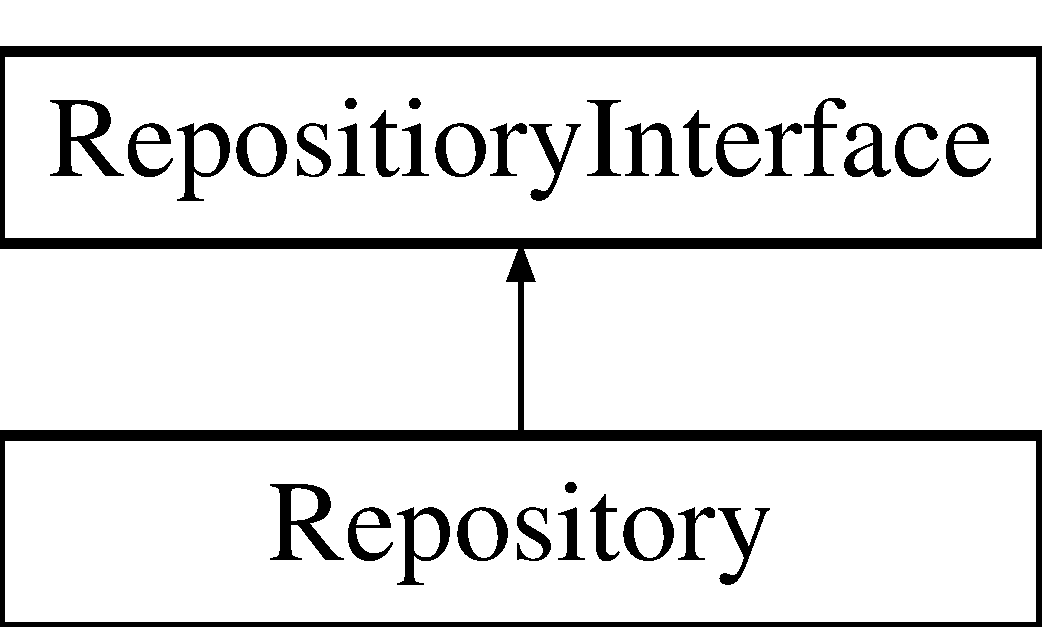
\includegraphics[height=2.000000cm]{de/daa/class_repositiory_interface}
\end{center}
\end{figure}
\subsection*{Public Member Functions}
\begin{DoxyCompactItemize}
\item 
virtual std\+::vector$<$ std\+::shared\+\_\+ptr$<$ \hyperlink{class_scene}{Scene} $>$ $>$ \hyperlink{class_repositiory_interface_a29a0f0fadd317082cb504bbb1161d50d}{get\+Game\+Scenes} () const =0
\begin{DoxyCompactList}\small\item\em Constructs the various Scenes required for the game implementation. \end{DoxyCompactList}\item 
virtual std\+::shared\+\_\+ptr$<$ \hyperlink{class_game_object}{Game\+Object} $>$ \hyperlink{class_repositiory_interface_a7341b8009f262949e26759327b0a8ae4}{get\+Game\+Objectby\+Type\+During\+Runtime} (Game\+Object\+Type objtype) const =0
\begin{DoxyCompactList}\small\item\em Used to Construct Game\+Objects that are only created once the game is already running. \end{DoxyCompactList}\item 
virtual std\+::vector$<$ unsigned int $>$ \hyperlink{class_repositiory_interface_a428e935faa2fd5790cbccc09f1066ef6}{get\+Game\+Screen\+Size} () const =0
\begin{DoxyCompactList}\small\item\em Returns the Screen Size of the game. \end{DoxyCompactList}\item 
virtual std\+::string \hyperlink{class_repositiory_interface_aa40617b92b721ec087dd69f3986e9efd}{get\+Game\+Name} () const =0
\begin{DoxyCompactList}\small\item\em returns the name of the game \end{DoxyCompactList}\end{DoxyCompactItemize}


\subsection{Detailed Description}
Repository\+Interface provides the game systems access to the database layer and the information it contains. Is also responsible for constructing the objects and Scenes used within the game. 

\subsection{Member Function Documentation}
\mbox{\Hypertarget{class_repositiory_interface_aa40617b92b721ec087dd69f3986e9efd}\label{class_repositiory_interface_aa40617b92b721ec087dd69f3986e9efd}} 
\index{Repositiory\+Interface@{Repositiory\+Interface}!get\+Game\+Name@{get\+Game\+Name}}
\index{get\+Game\+Name@{get\+Game\+Name}!Repositiory\+Interface@{Repositiory\+Interface}}
\subsubsection{\texorpdfstring{get\+Game\+Name()}{getGameName()}}
{\footnotesize\ttfamily virtual std\+::string Repositiory\+Interface\+::get\+Game\+Name (\begin{DoxyParamCaption}{ }\end{DoxyParamCaption}) const\hspace{0.3cm}{\ttfamily [pure virtual]}}



returns the name of the game 

\begin{DoxyReturn}{Returns}
Returns a string that represents the name of the game 
\end{DoxyReturn}


Implemented in \hyperlink{class_repository_a9bdfb4cab4ece2af1e45ef5ef06b9e49}{Repository}.

\mbox{\Hypertarget{class_repositiory_interface_a7341b8009f262949e26759327b0a8ae4}\label{class_repositiory_interface_a7341b8009f262949e26759327b0a8ae4}} 
\index{Repositiory\+Interface@{Repositiory\+Interface}!get\+Game\+Objectby\+Type\+During\+Runtime@{get\+Game\+Objectby\+Type\+During\+Runtime}}
\index{get\+Game\+Objectby\+Type\+During\+Runtime@{get\+Game\+Objectby\+Type\+During\+Runtime}!Repositiory\+Interface@{Repositiory\+Interface}}
\subsubsection{\texorpdfstring{get\+Game\+Objectby\+Type\+During\+Runtime()}{getGameObjectbyTypeDuringRuntime()}}
{\footnotesize\ttfamily virtual std\+::shared\+\_\+ptr$<$\hyperlink{class_game_object}{Game\+Object}$>$ Repositiory\+Interface\+::get\+Game\+Objectby\+Type\+During\+Runtime (\begin{DoxyParamCaption}\item[{Game\+Object\+Type}]{objtype }\end{DoxyParamCaption}) const\hspace{0.3cm}{\ttfamily [pure virtual]}}



Used to Construct Game\+Objects that are only created once the game is already running. 


\begin{DoxyParams}{Parameters}
{\em objtype} & The type of \hyperlink{class_game_object}{Game\+Object} that is required \\
\hline
\end{DoxyParams}
\begin{DoxyReturn}{Returns}
Returns the desired \hyperlink{class_game_object}{Game\+Object} 
\end{DoxyReturn}


Implemented in \hyperlink{class_repository_ab239e9b04db0524e168d54201bcd7076}{Repository}.

\mbox{\Hypertarget{class_repositiory_interface_a29a0f0fadd317082cb504bbb1161d50d}\label{class_repositiory_interface_a29a0f0fadd317082cb504bbb1161d50d}} 
\index{Repositiory\+Interface@{Repositiory\+Interface}!get\+Game\+Scenes@{get\+Game\+Scenes}}
\index{get\+Game\+Scenes@{get\+Game\+Scenes}!Repositiory\+Interface@{Repositiory\+Interface}}
\subsubsection{\texorpdfstring{get\+Game\+Scenes()}{getGameScenes()}}
{\footnotesize\ttfamily virtual std\+::vector$<$std\+::shared\+\_\+ptr$<$\hyperlink{class_scene}{Scene}$>$ $>$ Repositiory\+Interface\+::get\+Game\+Scenes (\begin{DoxyParamCaption}{ }\end{DoxyParamCaption}) const\hspace{0.3cm}{\ttfamily [pure virtual]}}



Constructs the various Scenes required for the game implementation. 

\begin{DoxyReturn}{Returns}
Returns a Vector of shared pointers of Scenes that are to exist in the game 
\end{DoxyReturn}


Implemented in \hyperlink{class_repository_ad49505f4ec3a15d0812ede7ff82b8be2}{Repository}.

\mbox{\Hypertarget{class_repositiory_interface_a428e935faa2fd5790cbccc09f1066ef6}\label{class_repositiory_interface_a428e935faa2fd5790cbccc09f1066ef6}} 
\index{Repositiory\+Interface@{Repositiory\+Interface}!get\+Game\+Screen\+Size@{get\+Game\+Screen\+Size}}
\index{get\+Game\+Screen\+Size@{get\+Game\+Screen\+Size}!Repositiory\+Interface@{Repositiory\+Interface}}
\subsubsection{\texorpdfstring{get\+Game\+Screen\+Size()}{getGameScreenSize()}}
{\footnotesize\ttfamily virtual std\+::vector$<$unsigned int$>$ Repositiory\+Interface\+::get\+Game\+Screen\+Size (\begin{DoxyParamCaption}{ }\end{DoxyParamCaption}) const\hspace{0.3cm}{\ttfamily [pure virtual]}}



Returns the Screen Size of the game. 

\begin{DoxyReturn}{Returns}
returns a vector where the first element is the x Screen Size value and the second element is the y Screen Size value 
\end{DoxyReturn}


Implemented in \hyperlink{class_repository_ab369b3a1d2957b2bd3130c8c348343dd}{Repository}.



The documentation for this class was generated from the following file\+:\begin{DoxyCompactItemize}
\item 
D\+:/\+Users/\+Tim-\/\+P\+C/\+Documents/\+Software\+\_\+\+I\+I/\+Project/\+Project\+Files/game-\/source-\/code/\+Back\+End\+Systems/Repository\+Interface.\+h\end{DoxyCompactItemize}

\hypertarget{class_repository}{}\section{Repository Class Reference}
\label{class_repository}\index{Repository@{Repository}}


\hyperlink{class_repository}{Repository} object used to create the specific scenes and objects defined for the current game implementation.  




{\ttfamily \#include $<$Repository.\+h$>$}

Inheritance diagram for Repository\+:\begin{figure}[H]
\begin{center}
\leavevmode
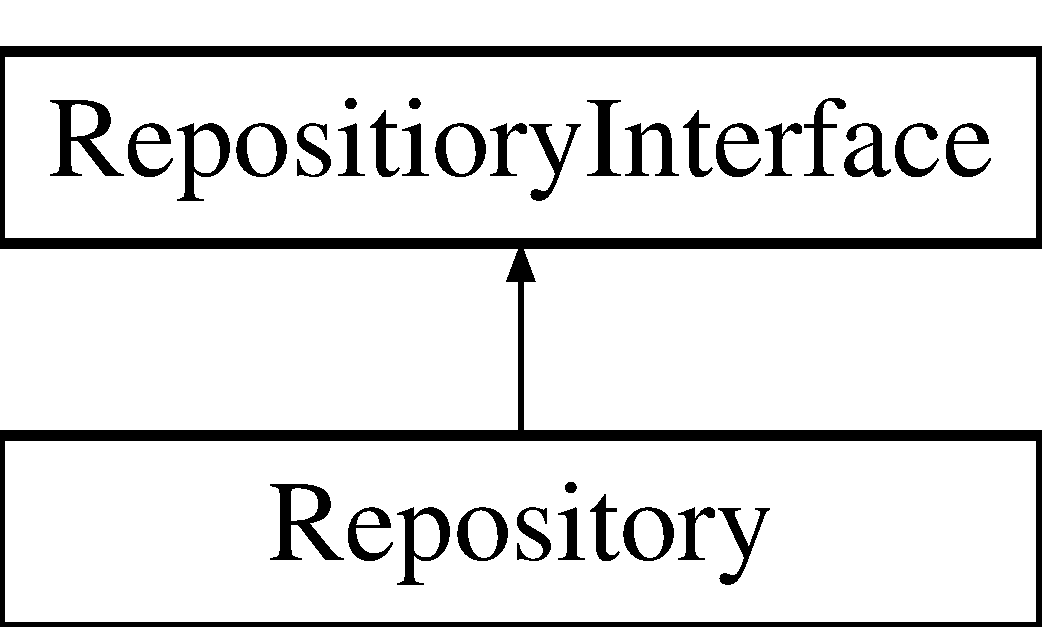
\includegraphics[height=2.000000cm]{da/d12/class_repository}
\end{center}
\end{figure}
\subsection*{Public Member Functions}
\begin{DoxyCompactItemize}
\item 
\hyperlink{class_repository_a0464c81256d66e31e9d5849d3ae0dfb2}{Repository} (std\+::shared\+\_\+ptr$<$ \hyperlink{class_data_mapper_interface}{Data\+Mapper\+Interface} $>$ data\+Mapper, std\+::shared\+\_\+ptr$<$ \hyperlink{class_database_interface}{Database\+Interface} $>$ runtime\+\_\+database)
\begin{DoxyCompactList}\small\item\em Constructs the repository object used by the game to create the various Game\+Objects and Scenes for the current game. \end{DoxyCompactList}\item 
virtual std\+::shared\+\_\+ptr$<$ \hyperlink{class_game_object}{Game\+Object} $>$ \hyperlink{class_repository_ab239e9b04db0524e168d54201bcd7076}{get\+Game\+Objectby\+Type\+During\+Runtime} (Game\+Object\+Type objtype) const override
\begin{DoxyCompactList}\small\item\em Used to generate a specific \hyperlink{class_game_object}{Game\+Object} during runtime of the game, is only defined for the various game\+Objects that are created during game runtime. \end{DoxyCompactList}\item 
virtual std\+::vector$<$ std\+::shared\+\_\+ptr$<$ \hyperlink{class_scene}{Scene} $>$ $>$ \hyperlink{class_repository_ad49505f4ec3a15d0812ede7ff82b8be2}{get\+Game\+Scenes} () const override
\begin{DoxyCompactList}\small\item\em Used to create the various scenes for the game. \end{DoxyCompactList}\item 
virtual std\+::vector$<$ unsigned int $>$ \hyperlink{class_repository_ab369b3a1d2957b2bd3130c8c348343dd}{get\+Game\+Screen\+Size} () const override
\begin{DoxyCompactList}\small\item\em Obtains the Size of the Screen from the \hyperlink{class_database_interface}{Database\+Interface}. \end{DoxyCompactList}\item 
virtual std\+::string \hyperlink{class_repository_a9bdfb4cab4ece2af1e45ef5ef06b9e49}{get\+Game\+Name} () const override
\begin{DoxyCompactList}\small\item\em Obtains the game name from the \hyperlink{class_database_interface}{Database\+Interface}. \end{DoxyCompactList}\end{DoxyCompactItemize}
\subsection*{Private Attributes}
\begin{DoxyCompactItemize}
\item 
std\+::shared\+\_\+ptr$<$ \hyperlink{class_data_mapper_interface}{Data\+Mapper\+Interface} $>$ \hyperlink{class_repository_a0bcbb13dbddc52d69c4b2d46a7730023}{\+\_\+data\+Mapper}
\item 
std\+::shared\+\_\+ptr$<$ \hyperlink{class_database_interface}{Database\+Interface} $>$ \hyperlink{class_repository_afe9b5f2e11e176745c227276c07bcdcb}{\+\_\+runtime\+\_\+database}
\end{DoxyCompactItemize}


\subsection{Detailed Description}
\hyperlink{class_repository}{Repository} object used to create the specific scenes and objects defined for the current game implementation. 

\subsection{Constructor \& Destructor Documentation}
\mbox{\Hypertarget{class_repository_a0464c81256d66e31e9d5849d3ae0dfb2}\label{class_repository_a0464c81256d66e31e9d5849d3ae0dfb2}} 
\index{Repository@{Repository}!Repository@{Repository}}
\index{Repository@{Repository}!Repository@{Repository}}
\subsubsection{\texorpdfstring{Repository()}{Repository()}}
{\footnotesize\ttfamily Repository\+::\+Repository (\begin{DoxyParamCaption}\item[{std\+::shared\+\_\+ptr$<$ \hyperlink{class_data_mapper_interface}{Data\+Mapper\+Interface} $>$}]{data\+Mapper,  }\item[{std\+::shared\+\_\+ptr$<$ \hyperlink{class_database_interface}{Database\+Interface} $>$}]{runtime\+\_\+database }\end{DoxyParamCaption})}



Constructs the repository object used by the game to create the various Game\+Objects and Scenes for the current game. 


\begin{DoxyParams}{Parameters}
{\em datamapper} & the \hyperlink{class_data_mapper_interface}{Data\+Mapper\+Interface} used to update the \+\_\+runtime\+\_\+database \\
\hline
{\em runtime\+\_\+database} & The \hyperlink{class_database_interface}{Database\+Interface} that stores the information of the game during game runtime \\
\hline
\end{DoxyParams}


\subsection{Member Function Documentation}
\mbox{\Hypertarget{class_repository_a9bdfb4cab4ece2af1e45ef5ef06b9e49}\label{class_repository_a9bdfb4cab4ece2af1e45ef5ef06b9e49}} 
\index{Repository@{Repository}!get\+Game\+Name@{get\+Game\+Name}}
\index{get\+Game\+Name@{get\+Game\+Name}!Repository@{Repository}}
\subsubsection{\texorpdfstring{get\+Game\+Name()}{getGameName()}}
{\footnotesize\ttfamily std\+::string Repository\+::get\+Game\+Name (\begin{DoxyParamCaption}{ }\end{DoxyParamCaption}) const\hspace{0.3cm}{\ttfamily [override]}, {\ttfamily [virtual]}}



Obtains the game name from the \hyperlink{class_database_interface}{Database\+Interface}. 

\begin{DoxyReturn}{Returns}
Returns the Name of the Game as a string 
\end{DoxyReturn}


Implements \hyperlink{class_repositiory_interface_aa40617b92b721ec087dd69f3986e9efd}{Repositiory\+Interface}.

\mbox{\Hypertarget{class_repository_ab239e9b04db0524e168d54201bcd7076}\label{class_repository_ab239e9b04db0524e168d54201bcd7076}} 
\index{Repository@{Repository}!get\+Game\+Objectby\+Type\+During\+Runtime@{get\+Game\+Objectby\+Type\+During\+Runtime}}
\index{get\+Game\+Objectby\+Type\+During\+Runtime@{get\+Game\+Objectby\+Type\+During\+Runtime}!Repository@{Repository}}
\subsubsection{\texorpdfstring{get\+Game\+Objectby\+Type\+During\+Runtime()}{getGameObjectbyTypeDuringRuntime()}}
{\footnotesize\ttfamily std\+::shared\+\_\+ptr$<$ \hyperlink{class_game_object}{Game\+Object} $>$ Repository\+::get\+Game\+Objectby\+Type\+During\+Runtime (\begin{DoxyParamCaption}\item[{Game\+Object\+Type}]{objtype }\end{DoxyParamCaption}) const\hspace{0.3cm}{\ttfamily [override]}, {\ttfamily [virtual]}}



Used to generate a specific \hyperlink{class_game_object}{Game\+Object} during runtime of the game, is only defined for the various game\+Objects that are created during game runtime. 


\begin{DoxyParams}{Parameters}
{\em objtype} & The Game\+Object\+Type that represents the object that needs to be created \\
\hline
\end{DoxyParams}
\begin{DoxyReturn}{Returns}
Returns the desired \hyperlink{class_game_object}{Game\+Object} 
\end{DoxyReturn}


Implements \hyperlink{class_repositiory_interface_a7341b8009f262949e26759327b0a8ae4}{Repositiory\+Interface}.

\mbox{\Hypertarget{class_repository_ad49505f4ec3a15d0812ede7ff82b8be2}\label{class_repository_ad49505f4ec3a15d0812ede7ff82b8be2}} 
\index{Repository@{Repository}!get\+Game\+Scenes@{get\+Game\+Scenes}}
\index{get\+Game\+Scenes@{get\+Game\+Scenes}!Repository@{Repository}}
\subsubsection{\texorpdfstring{get\+Game\+Scenes()}{getGameScenes()}}
{\footnotesize\ttfamily std\+::vector$<$ std\+::shared\+\_\+ptr$<$ \hyperlink{class_scene}{Scene} $>$ $>$ Repository\+::get\+Game\+Scenes (\begin{DoxyParamCaption}{ }\end{DoxyParamCaption}) const\hspace{0.3cm}{\ttfamily [override]}, {\ttfamily [virtual]}}



Used to create the various scenes for the game. 

\begin{DoxyReturn}{Returns}
Returns a Vector of shared pointers of Scenes that are to exist in the game 
\end{DoxyReturn}


Implements \hyperlink{class_repositiory_interface_a29a0f0fadd317082cb504bbb1161d50d}{Repositiory\+Interface}.

\mbox{\Hypertarget{class_repository_ab369b3a1d2957b2bd3130c8c348343dd}\label{class_repository_ab369b3a1d2957b2bd3130c8c348343dd}} 
\index{Repository@{Repository}!get\+Game\+Screen\+Size@{get\+Game\+Screen\+Size}}
\index{get\+Game\+Screen\+Size@{get\+Game\+Screen\+Size}!Repository@{Repository}}
\subsubsection{\texorpdfstring{get\+Game\+Screen\+Size()}{getGameScreenSize()}}
{\footnotesize\ttfamily std\+::vector$<$ unsigned int $>$ Repository\+::get\+Game\+Screen\+Size (\begin{DoxyParamCaption}{ }\end{DoxyParamCaption}) const\hspace{0.3cm}{\ttfamily [override]}, {\ttfamily [virtual]}}



Obtains the Size of the Screen from the \hyperlink{class_database_interface}{Database\+Interface}. 

\begin{DoxyReturn}{Returns}
Returns the Screen Size of the game 
\end{DoxyReturn}


Implements \hyperlink{class_repositiory_interface_a428e935faa2fd5790cbccc09f1066ef6}{Repositiory\+Interface}.



\subsection{Member Data Documentation}
\mbox{\Hypertarget{class_repository_a0bcbb13dbddc52d69c4b2d46a7730023}\label{class_repository_a0bcbb13dbddc52d69c4b2d46a7730023}} 
\index{Repository@{Repository}!\+\_\+data\+Mapper@{\+\_\+data\+Mapper}}
\index{\+\_\+data\+Mapper@{\+\_\+data\+Mapper}!Repository@{Repository}}
\subsubsection{\texorpdfstring{\+\_\+data\+Mapper}{\_dataMapper}}
{\footnotesize\ttfamily std\+::shared\+\_\+ptr$<$\hyperlink{class_data_mapper_interface}{Data\+Mapper\+Interface}$>$ Repository\+::\+\_\+data\+Mapper\hspace{0.3cm}{\ttfamily [private]}}

The \hyperlink{class_data_mapper_interface}{Data\+Mapper\+Interface} used to update the \+\_\+runtime\+\_\+database \mbox{\Hypertarget{class_repository_afe9b5f2e11e176745c227276c07bcdcb}\label{class_repository_afe9b5f2e11e176745c227276c07bcdcb}} 
\index{Repository@{Repository}!\+\_\+runtime\+\_\+database@{\+\_\+runtime\+\_\+database}}
\index{\+\_\+runtime\+\_\+database@{\+\_\+runtime\+\_\+database}!Repository@{Repository}}
\subsubsection{\texorpdfstring{\+\_\+runtime\+\_\+database}{\_runtime\_database}}
{\footnotesize\ttfamily std\+::shared\+\_\+ptr$<$\hyperlink{class_database_interface}{Database\+Interface}$>$ Repository\+::\+\_\+runtime\+\_\+database\hspace{0.3cm}{\ttfamily [private]}}

The \hyperlink{class_database_interface}{Database\+Interface} used to store the game object information at during runtime of the application 

The documentation for this class was generated from the following files\+:\begin{DoxyCompactItemize}
\item 
C\+:/\+Users/\+Tim/\+Documents/\+Software\+Dev/\+Software\+Project/\+Project\+Files/game-\/source-\/code/\+Back\+End\+Systems/Repository.\+h\item 
C\+:/\+Users/\+Tim/\+Documents/\+Software\+Dev/\+Software\+Project/\+Project\+Files/game-\/source-\/code/\+Back\+End\+Systems/Repository.\+cpp\end{DoxyCompactItemize}

\hypertarget{structrt_vector}{}\section{rt\+Vector Struct Reference}
\label{structrt_vector}\index{rt\+Vector@{rt\+Vector}}
\subsection*{Public Member Functions}
\begin{DoxyCompactItemize}
\item 
\mbox{\Hypertarget{structrt_vector_a97268ebbcad1df534201f5225f7ccbb0}\label{structrt_vector_a97268ebbcad1df534201f5225f7ccbb0}} 
{\bfseries rt\+Vector} (double R, double T)
\end{DoxyCompactItemize}
\subsection*{Public Attributes}
\begin{DoxyCompactItemize}
\item 
\mbox{\Hypertarget{structrt_vector_aae522780f6ddbf1a8d45dc69e89ab1b8}\label{structrt_vector_aae522780f6ddbf1a8d45dc69e89ab1b8}} 
double {\bfseries r}
\item 
\mbox{\Hypertarget{structrt_vector_a8ab4ea9b5dfa69f99fcb5e62dd9b138d}\label{structrt_vector_a8ab4ea9b5dfa69f99fcb5e62dd9b138d}} 
double {\bfseries t}
\end{DoxyCompactItemize}


The documentation for this struct was generated from the following file\+:\begin{DoxyCompactItemize}
\item 
D\+:/\+Users/\+Tim-\/\+P\+C/\+Documents/\+Software\+\_\+\+I\+I/\+Project/\+Project\+Files/game-\/source-\/code/Vector2\+D.\+h\end{DoxyCompactItemize}

\hypertarget{class_run_time_database}{}\section{Run\+Time\+Database Class Reference}
\label{class_run_time_database}\index{Run\+Time\+Database@{Run\+Time\+Database}}


This class is responsible for storing a hashtable containing the various information about the different gameobjects used in the game. It also stores the information regarding the game state and provides access functionality as defined by the \hyperlink{class_database_interface}{Database\+Interface} Interface class.  




{\ttfamily \#include $<$Run\+Time\+Database.\+h$>$}

Inheritance diagram for Run\+Time\+Database\+:\begin{figure}[H]
\begin{center}
\leavevmode
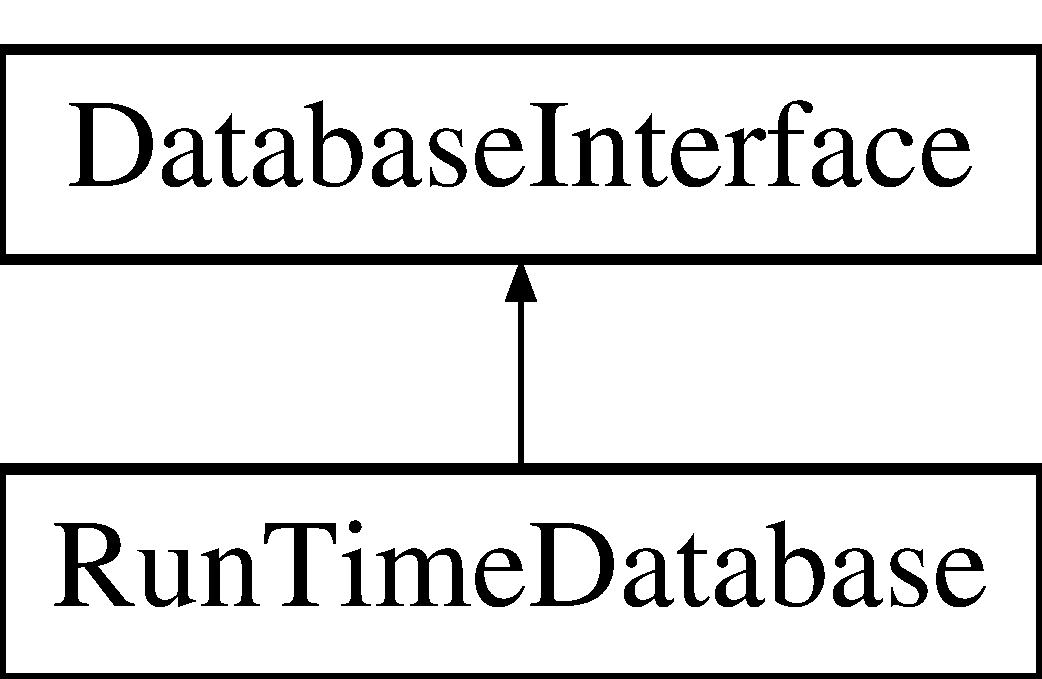
\includegraphics[height=2.000000cm]{de/d2f/class_run_time_database}
\end{center}
\end{figure}
\subsection*{Public Member Functions}
\begin{DoxyCompactItemize}
\item 
virtual \hyperlink{struct_game_object_data}{Game\+Object\+Data} \hyperlink{class_run_time_database_aabe246e23f6f8ded2c3b61fcfa396f2a}{get\+Game\+Object\+Data} (std\+::string ID) override
\begin{DoxyCompactList}\small\item\em Used to obtain the various data that relates to the different Game\+Objects used inside the game. \end{DoxyCompactList}\item 
virtual \hyperlink{struct_game_state_data}{Game\+State\+Data} \hyperlink{class_run_time_database_a15d6105d3d772f604c42813e50ba4ee3}{get\+Game\+State\+Data} () override
\begin{DoxyCompactList}\small\item\em Gets the data about the current state of the game. \end{DoxyCompactList}\item 
virtual void \hyperlink{class_run_time_database_af18f09a5166adc6ab075034e272e9c8d}{set\+Game\+State\+Data} (\hyperlink{struct_game_state_data}{Game\+State\+Data} game\+State\+Data) override
\begin{DoxyCompactList}\small\item\em Sets the \hyperlink{struct_game_state_data}{Game\+State\+Data} inside of the database. \end{DoxyCompactList}\item 
virtual void \hyperlink{class_run_time_database_a9d2c5c2f1eb4dc728d69b9c5dbd1c22d}{set\+Game\+Object\+Data} (std\+::string ID, \hyperlink{struct_game_object_data}{Game\+Object\+Data} game\+Object\+Data) override
\begin{DoxyCompactList}\small\item\em Sets the object data at the corresponding ID provided into the database. \end{DoxyCompactList}\end{DoxyCompactItemize}
\subsection*{Protected Attributes}
\begin{DoxyCompactItemize}
\item 
std\+::unordered\+\_\+map$<$ std\+::string, \hyperlink{struct_game_object_data}{Game\+Object\+Data} $>$ \hyperlink{class_run_time_database_aec15546ee0f7bf69bd1ba0a74656790d}{\+\_\+game\+Object\+Data}
\item 
\hyperlink{struct_game_state_data}{Game\+State\+Data} \hyperlink{class_run_time_database_a1d965e094a4035d1a6c28a566a29cb8e}{\+\_\+game\+State\+Data}
\end{DoxyCompactItemize}


\subsection{Detailed Description}
This class is responsible for storing a hashtable containing the various information about the different gameobjects used in the game. It also stores the information regarding the game state and provides access functionality as defined by the \hyperlink{class_database_interface}{Database\+Interface} Interface class. 

\subsection{Member Function Documentation}
\mbox{\Hypertarget{class_run_time_database_aabe246e23f6f8ded2c3b61fcfa396f2a}\label{class_run_time_database_aabe246e23f6f8ded2c3b61fcfa396f2a}} 
\index{Run\+Time\+Database@{Run\+Time\+Database}!get\+Game\+Object\+Data@{get\+Game\+Object\+Data}}
\index{get\+Game\+Object\+Data@{get\+Game\+Object\+Data}!Run\+Time\+Database@{Run\+Time\+Database}}
\subsubsection{\texorpdfstring{get\+Game\+Object\+Data()}{getGameObjectData()}}
{\footnotesize\ttfamily \hyperlink{struct_game_object_data}{Game\+Object\+Data} Run\+Time\+Database\+::get\+Game\+Object\+Data (\begin{DoxyParamCaption}\item[{std\+::string}]{ID }\end{DoxyParamCaption})\hspace{0.3cm}{\ttfamily [override]}, {\ttfamily [virtual]}}



Used to obtain the various data that relates to the different Game\+Objects used inside the game. 


\begin{DoxyParams}{Parameters}
{\em ID} & The speciic ID required to return the correct object data \\
\hline
\end{DoxyParams}
\begin{DoxyReturn}{Returns}
Returns the \hyperlink{struct_game_object_data}{Game\+Object\+Data} relating to the object defined by the ID 
\end{DoxyReturn}


Implements \hyperlink{class_database_interface_a515afa17b15a4b111ebc1a43e1d0218e}{Database\+Interface}.

\mbox{\Hypertarget{class_run_time_database_a15d6105d3d772f604c42813e50ba4ee3}\label{class_run_time_database_a15d6105d3d772f604c42813e50ba4ee3}} 
\index{Run\+Time\+Database@{Run\+Time\+Database}!get\+Game\+State\+Data@{get\+Game\+State\+Data}}
\index{get\+Game\+State\+Data@{get\+Game\+State\+Data}!Run\+Time\+Database@{Run\+Time\+Database}}
\subsubsection{\texorpdfstring{get\+Game\+State\+Data()}{getGameStateData()}}
{\footnotesize\ttfamily \hyperlink{struct_game_state_data}{Game\+State\+Data} Run\+Time\+Database\+::get\+Game\+State\+Data (\begin{DoxyParamCaption}{ }\end{DoxyParamCaption})\hspace{0.3cm}{\ttfamily [override]}, {\ttfamily [virtual]}}



Gets the data about the current state of the game. 

\begin{DoxyReturn}{Returns}
Returns the \hyperlink{struct_game_state_data}{Game\+State\+Data} which relates to the game, including the game screen size and name 
\end{DoxyReturn}


Implements \hyperlink{class_database_interface_a5972ccdce7669da4eef8ab82c69fe073}{Database\+Interface}.

\mbox{\Hypertarget{class_run_time_database_a9d2c5c2f1eb4dc728d69b9c5dbd1c22d}\label{class_run_time_database_a9d2c5c2f1eb4dc728d69b9c5dbd1c22d}} 
\index{Run\+Time\+Database@{Run\+Time\+Database}!set\+Game\+Object\+Data@{set\+Game\+Object\+Data}}
\index{set\+Game\+Object\+Data@{set\+Game\+Object\+Data}!Run\+Time\+Database@{Run\+Time\+Database}}
\subsubsection{\texorpdfstring{set\+Game\+Object\+Data()}{setGameObjectData()}}
{\footnotesize\ttfamily void Run\+Time\+Database\+::set\+Game\+Object\+Data (\begin{DoxyParamCaption}\item[{std\+::string}]{ID,  }\item[{\hyperlink{struct_game_object_data}{Game\+Object\+Data}}]{game\+Object\+Data }\end{DoxyParamCaption})\hspace{0.3cm}{\ttfamily [override]}, {\ttfamily [virtual]}}



Sets the object data at the corresponding ID provided into the database. 


\begin{DoxyParams}{Parameters}
{\em ID} & The ID of the object that neeeds to be set within the database \\
\hline
{\em game\+Object\+Data} & The \hyperlink{struct_game_object_data}{Game\+Object\+Data} stored \\
\hline
\end{DoxyParams}


Implements \hyperlink{class_database_interface_ae1914371cb425f71ba750f57f968b491}{Database\+Interface}.

\mbox{\Hypertarget{class_run_time_database_af18f09a5166adc6ab075034e272e9c8d}\label{class_run_time_database_af18f09a5166adc6ab075034e272e9c8d}} 
\index{Run\+Time\+Database@{Run\+Time\+Database}!set\+Game\+State\+Data@{set\+Game\+State\+Data}}
\index{set\+Game\+State\+Data@{set\+Game\+State\+Data}!Run\+Time\+Database@{Run\+Time\+Database}}
\subsubsection{\texorpdfstring{set\+Game\+State\+Data()}{setGameStateData()}}
{\footnotesize\ttfamily void Run\+Time\+Database\+::set\+Game\+State\+Data (\begin{DoxyParamCaption}\item[{\hyperlink{struct_game_state_data}{Game\+State\+Data}}]{game\+State\+Data }\end{DoxyParamCaption})\hspace{0.3cm}{\ttfamily [override]}, {\ttfamily [virtual]}}



Sets the \hyperlink{struct_game_state_data}{Game\+State\+Data} inside of the database. 


\begin{DoxyParams}{Parameters}
{\em game\+State\+Data} & The specific \hyperlink{struct_game_state_data}{Game\+State\+Data} stored within the database \\
\hline
\end{DoxyParams}


Implements \hyperlink{class_database_interface_a0b2f4402583b6ab31c70c713d72ceede}{Database\+Interface}.



\subsection{Member Data Documentation}
\mbox{\Hypertarget{class_run_time_database_aec15546ee0f7bf69bd1ba0a74656790d}\label{class_run_time_database_aec15546ee0f7bf69bd1ba0a74656790d}} 
\index{Run\+Time\+Database@{Run\+Time\+Database}!\+\_\+game\+Object\+Data@{\+\_\+game\+Object\+Data}}
\index{\+\_\+game\+Object\+Data@{\+\_\+game\+Object\+Data}!Run\+Time\+Database@{Run\+Time\+Database}}
\subsubsection{\texorpdfstring{\+\_\+game\+Object\+Data}{\_gameObjectData}}
{\footnotesize\ttfamily std\+::unordered\+\_\+map$<$std\+::string, \hyperlink{struct_game_object_data}{Game\+Object\+Data}$>$ Run\+Time\+Database\+::\+\_\+game\+Object\+Data\hspace{0.3cm}{\ttfamily [protected]}}

Hash Table datastructure used to store the \hyperlink{class_game_object}{Game\+Object} information in the form of \hyperlink{struct_game_object_data}{Game\+Object\+Data} \mbox{\Hypertarget{class_run_time_database_a1d965e094a4035d1a6c28a566a29cb8e}\label{class_run_time_database_a1d965e094a4035d1a6c28a566a29cb8e}} 
\index{Run\+Time\+Database@{Run\+Time\+Database}!\+\_\+game\+State\+Data@{\+\_\+game\+State\+Data}}
\index{\+\_\+game\+State\+Data@{\+\_\+game\+State\+Data}!Run\+Time\+Database@{Run\+Time\+Database}}
\subsubsection{\texorpdfstring{\+\_\+game\+State\+Data}{\_gameStateData}}
{\footnotesize\ttfamily \hyperlink{struct_game_state_data}{Game\+State\+Data} Run\+Time\+Database\+::\+\_\+game\+State\+Data\hspace{0.3cm}{\ttfamily [protected]}}

Variable that stores the information about the game state 

The documentation for this class was generated from the following files\+:\begin{DoxyCompactItemize}
\item 
C\+:/\+Users/\+Tim/\+Documents/\+Software\+Dev/\+Software\+Project/\+Project\+Files/game-\/source-\/code/\+Back\+End\+Systems/Run\+Time\+Database.\+h\item 
C\+:/\+Users/\+Tim/\+Documents/\+Software\+Dev/\+Software\+Project/\+Project\+Files/game-\/source-\/code/\+Back\+End\+Systems/Run\+Time\+Database.\+cpp\end{DoxyCompactItemize}

\hypertarget{class_scene}{}\section{Scene Class Reference}
\label{class_scene}\index{Scene@{Scene}}
Inheritance diagram for Scene\+:\begin{figure}[H]
\begin{center}
\leavevmode
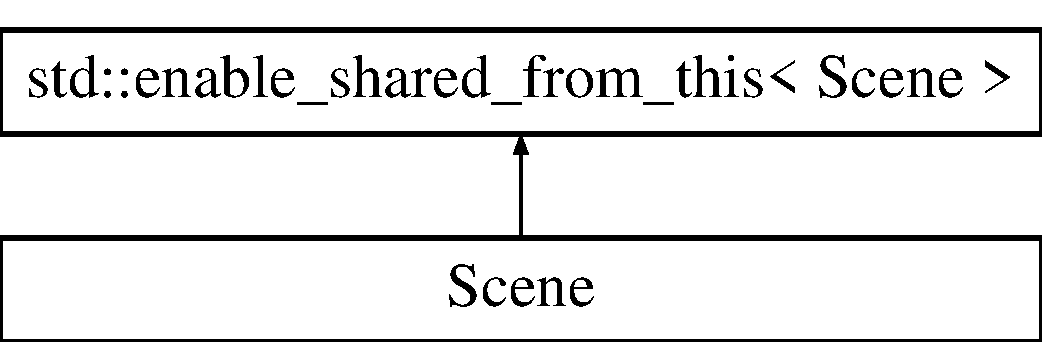
\includegraphics[height=2.000000cm]{d6/db5/class_scene}
\end{center}
\end{figure}
\subsection*{Public Member Functions}
\begin{DoxyCompactItemize}
\item 
\mbox{\Hypertarget{class_scene_a0caa1ccf717fe21059f20b0c4a57cde6}\label{class_scene_a0caa1ccf717fe21059f20b0c4a57cde6}} 
\hyperlink{class_scene_a0caa1ccf717fe21059f20b0c4a57cde6}{Scene} (const \hyperlink{class_scene}{Scene} \&rhs)
\begin{DoxyCompactList}\small\item\em Currently needs to be fixed. \end{DoxyCompactList}\item 
\mbox{\Hypertarget{class_scene_a1d902efeacc113ceb2dd79a976b04a77}\label{class_scene_a1d902efeacc113ceb2dd79a976b04a77}} 
void {\bfseries Scene\+Update} ()
\item 
void \hyperlink{class_scene_a3dd730cba4a22bf75e54c4b644c26976}{Instantiate} (shared\+\_\+ptr$<$ \hyperlink{class_game_object}{Game\+Object} $>$ game\+Obj)
\item 
\mbox{\Hypertarget{class_scene_ae418f788bfbf2551d89e907d1d4cf2f6}\label{class_scene_ae418f788bfbf2551d89e907d1d4cf2f6}} 
void {\bfseries Destroy\+Game\+Object} (game\+Obj\+\_\+ptr game\+Object)
\item 
\mbox{\Hypertarget{class_scene_a0696711d2b1452f3d6f42f7a92f4218d}\label{class_scene_a0696711d2b1452f3d6f42f7a92f4218d}} 
std\+::vector$<$ game\+Obj\+\_\+ptr $>$ {\bfseries get\+Game\+Object\+List} () const
\item 
\mbox{\Hypertarget{class_scene_a64a47e6503f634ea2b76fa2078538716}\label{class_scene_a64a47e6503f634ea2b76fa2078538716}} 
\hyperlink{class_scene}{Scene} \& {\bfseries operator=} (const \hyperlink{class_scene}{Scene} \&rhs)
\end{DoxyCompactItemize}
\subsection*{Public Attributes}
\begin{DoxyCompactItemize}
\item 
\mbox{\Hypertarget{class_scene_a29183cf37f5227ea9a82d2a15c42336c}\label{class_scene_a29183cf37f5227ea9a82d2a15c42336c}} 
std\+::mutex {\bfseries \+\_\+game\+Object\+\_\+list\+\_\+mutex}
\end{DoxyCompactItemize}
\subsection*{Private Attributes}
\begin{DoxyCompactItemize}
\item 
std\+::vector$<$ game\+Obj\+\_\+ptr $>$ \hyperlink{class_scene_af1956432917d14b0a0b26103dbcb5bcd}{\+\_\+game\+Object\+\_\+list}
\end{DoxyCompactItemize}


\subsection{Member Function Documentation}
\mbox{\Hypertarget{class_scene_a3dd730cba4a22bf75e54c4b644c26976}\label{class_scene_a3dd730cba4a22bf75e54c4b644c26976}} 
\index{Scene@{Scene}!Instantiate@{Instantiate}}
\index{Instantiate@{Instantiate}!Scene@{Scene}}
\subsubsection{\texorpdfstring{Instantiate()}{Instantiate()}}
{\footnotesize\ttfamily void Scene\+::\+Instantiate (\begin{DoxyParamCaption}\item[{shared\+\_\+ptr$<$ \hyperlink{class_game_object}{Game\+Object} $>$}]{game\+Obj }\end{DoxyParamCaption})}

Seems redundant to do duplicate the game object pointer 

\subsection{Member Data Documentation}
\mbox{\Hypertarget{class_scene_af1956432917d14b0a0b26103dbcb5bcd}\label{class_scene_af1956432917d14b0a0b26103dbcb5bcd}} 
\index{Scene@{Scene}!\+\_\+game\+Object\+\_\+list@{\+\_\+game\+Object\+\_\+list}}
\index{\+\_\+game\+Object\+\_\+list@{\+\_\+game\+Object\+\_\+list}!Scene@{Scene}}
\subsubsection{\texorpdfstring{\+\_\+game\+Object\+\_\+list}{\_gameObject\_list}}
{\footnotesize\ttfamily std\+::vector$<$game\+Obj\+\_\+ptr$>$ Scene\+::\+\_\+game\+Object\+\_\+list\hspace{0.3cm}{\ttfamily [private]}}

would be better to use a doubly linked list instead of a vector since it has a better time effeciency when it deals with insertion and deletion of elements 

The documentation for this class was generated from the following files\+:\begin{DoxyCompactItemize}
\item 
D\+:/\+Users/\+Tim-\/\+P\+C/\+Documents/\+Software\+\_\+\+I\+I/\+Project/\+Project\+Files/game-\/source-\/code/\+Front\+End\+Systems/Scene.\+h\item 
D\+:/\+Users/\+Tim-\/\+P\+C/\+Documents/\+Software\+\_\+\+I\+I/\+Project/\+Project\+Files/game-\/source-\/code/\+Front\+End\+Systems/Scene.\+cpp\end{DoxyCompactItemize}

\hypertarget{class_scene_doesnt_exist}{}\section{Scene\+Doesnt\+Exist Class Reference}
\label{class_scene_doesnt_exist}\index{Scene\+Doesnt\+Exist@{Scene\+Doesnt\+Exist}}


Exception thrown if a scene does not exist at the specific index that is requested.  




{\ttfamily \#include $<$Game\+Manager.\+h$>$}



\subsection{Detailed Description}
Exception thrown if a scene does not exist at the specific index that is requested. 

The documentation for this class was generated from the following file\+:\begin{DoxyCompactItemize}
\item 
D\+:/\+Users/\+Tim-\/\+P\+C/\+Documents/\+Software\+\_\+\+I\+I/\+Project/\+Project\+Files/game-\/source-\/code/\+Back\+End\+Systems/Game\+Manager.\+h\end{DoxyCompactItemize}

\hypertarget{class_scene_factory}{}\section{Scene\+Factory Class Reference}
\label{class_scene_factory}\index{Scene\+Factory@{Scene\+Factory}}


Base class used to create the various scenes within the game.  




{\ttfamily \#include $<$Scene\+Factory.\+h$>$}

Inheritance diagram for Scene\+Factory\+:\begin{figure}[H]
\begin{center}
\leavevmode
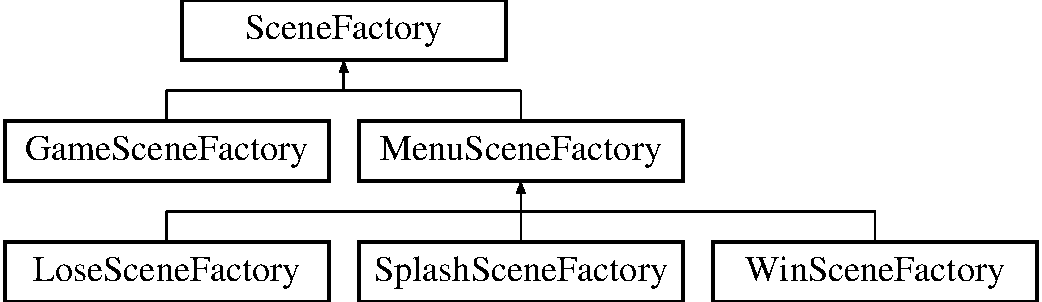
\includegraphics[height=3.000000cm]{d8/d70/class_scene_factory}
\end{center}
\end{figure}
\subsection*{Public Member Functions}
\begin{DoxyCompactItemize}
\item 
std\+::shared\+\_\+ptr$<$ \hyperlink{class_scene}{Scene} $>$ \hyperlink{class_scene_factory_a9721384ff0d8703f0ef28bf9061fe402}{get\+Scene} (std\+::shared\+\_\+ptr$<$ \hyperlink{class_database_interface}{Database\+Interface} $>$ database) const
\begin{DoxyCompactList}\small\item\em Constructs the \hyperlink{class_scene}{Scene} defined by the type of \hyperlink{class_scene}{Scene} factory. \end{DoxyCompactList}\end{DoxyCompactItemize}
\subsection*{Protected Member Functions}
\begin{DoxyCompactItemize}
\item 
virtual std\+::list$<$ std\+::shared\+\_\+ptr$<$ \hyperlink{class_game_object}{Game\+Object} $>$ $>$ \hyperlink{class_scene_factory_a2c8541230e95df49d2ab39b7c6ecdb78}{get\+Game\+Obect\+List} (std\+::shared\+\_\+ptr$<$ \hyperlink{class_database_interface}{Database\+Interface} $>$ database) const =0
\begin{DoxyCompactList}\small\item\em Returns the game\+Object list required for the construction of the specific \hyperlink{class_scene}{Scene}. \end{DoxyCompactList}\end{DoxyCompactItemize}


\subsection{Detailed Description}
Base class used to create the various scenes within the game. 

\subsection{Member Function Documentation}
\mbox{\Hypertarget{class_scene_factory_a2c8541230e95df49d2ab39b7c6ecdb78}\label{class_scene_factory_a2c8541230e95df49d2ab39b7c6ecdb78}} 
\index{Scene\+Factory@{Scene\+Factory}!get\+Game\+Obect\+List@{get\+Game\+Obect\+List}}
\index{get\+Game\+Obect\+List@{get\+Game\+Obect\+List}!Scene\+Factory@{Scene\+Factory}}
\subsubsection{\texorpdfstring{get\+Game\+Obect\+List()}{getGameObectList()}}
{\footnotesize\ttfamily virtual std\+::list$<$std\+::shared\+\_\+ptr$<$\hyperlink{class_game_object}{Game\+Object}$>$ $>$ Scene\+Factory\+::get\+Game\+Obect\+List (\begin{DoxyParamCaption}\item[{std\+::shared\+\_\+ptr$<$ \hyperlink{class_database_interface}{Database\+Interface} $>$}]{database }\end{DoxyParamCaption}) const\hspace{0.3cm}{\ttfamily [protected]}, {\ttfamily [pure virtual]}}



Returns the game\+Object list required for the construction of the specific \hyperlink{class_scene}{Scene}. 


\begin{DoxyParams}{Parameters}
{\em database} & The \hyperlink{class_database_interface}{Database\+Interface} that contains the information about the various Game\+Objects \\
\hline
\end{DoxyParams}


Implemented in \hyperlink{class_menu_scene_factory_ade1881c377fa61d1d8fa11c1d30f4ddd}{Menu\+Scene\+Factory}, and \hyperlink{class_game_scene_factory_a2db801c1a1703a14a00c7b6e8bdca5b0}{Game\+Scene\+Factory}.

\mbox{\Hypertarget{class_scene_factory_a9721384ff0d8703f0ef28bf9061fe402}\label{class_scene_factory_a9721384ff0d8703f0ef28bf9061fe402}} 
\index{Scene\+Factory@{Scene\+Factory}!get\+Scene@{get\+Scene}}
\index{get\+Scene@{get\+Scene}!Scene\+Factory@{Scene\+Factory}}
\subsubsection{\texorpdfstring{get\+Scene()}{getScene()}}
{\footnotesize\ttfamily std\+::shared\+\_\+ptr$<$ \hyperlink{class_scene}{Scene} $>$ Scene\+Factory\+::get\+Scene (\begin{DoxyParamCaption}\item[{std\+::shared\+\_\+ptr$<$ \hyperlink{class_database_interface}{Database\+Interface} $>$}]{database }\end{DoxyParamCaption}) const}



Constructs the \hyperlink{class_scene}{Scene} defined by the type of \hyperlink{class_scene}{Scene} factory. 


\begin{DoxyParams}{Parameters}
{\em database} & The \hyperlink{class_database_interface}{Database\+Interface} that contains the information about the various Game\+Objects \\
\hline
\end{DoxyParams}
\begin{DoxyReturn}{Returns}
Returns the Constructed \hyperlink{class_scene}{Scene} 
\end{DoxyReturn}


The documentation for this class was generated from the following files\+:\begin{DoxyCompactItemize}
\item 
C\+:/\+Users/\+Tim/\+Documents/\+Software\+Dev/\+Software\+Project/\+Project\+Files/game-\/source-\/code/\+Back\+End\+Systems/Scene\+Factory.\+h\item 
C\+:/\+Users/\+Tim/\+Documents/\+Software\+Dev/\+Software\+Project/\+Project\+Files/game-\/source-\/code/\+Back\+End\+Systems/Scene\+Factory.\+cpp\end{DoxyCompactItemize}

\hypertarget{class_shoot_interface}{}\section{Shoot\+Interface Class Reference}
\label{class_shoot_interface}\index{Shoot\+Interface@{Shoot\+Interface}}


The Interface used to define the various methods of creating and shooting \hyperlink{class_projectile}{Projectile} objects.  




{\ttfamily \#include $<$Shoot\+Interface.\+h$>$}

Inheritance diagram for Shoot\+Interface\+:\begin{figure}[H]
\begin{center}
\leavevmode
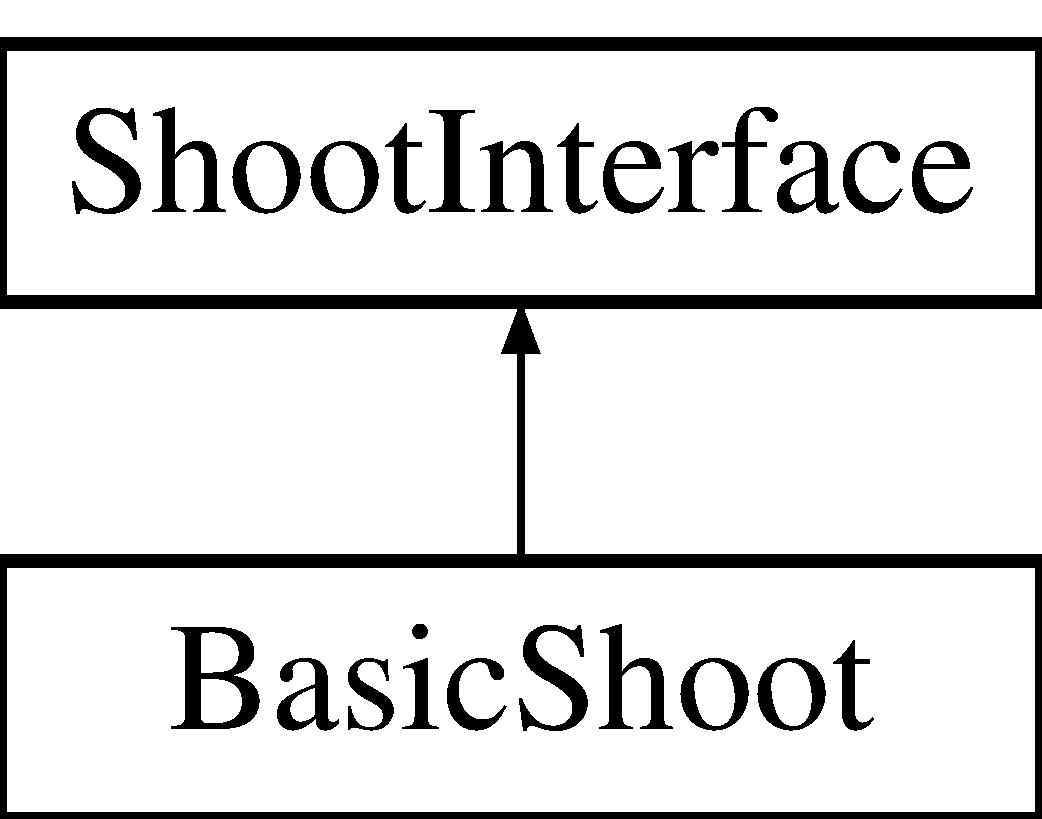
\includegraphics[height=2.000000cm]{d9/d8a/class_shoot_interface}
\end{center}
\end{figure}
\subsection*{Public Member Functions}
\begin{DoxyCompactItemize}
\item 
virtual void \hyperlink{class_shoot_interface_a67205cc4e2fed90fa8c1ec93b30b864d}{Shoot} (\hyperlink{class_vector2_d}{Vector2D} start\+Position, \hyperlink{class_vector2_d}{Vector2D} target, std\+::shared\+\_\+ptr$<$ \hyperlink{class_scene}{Scene} $>$ scene)=0
\begin{DoxyCompactList}\small\item\em Shoots a \hyperlink{class_projectile}{Projectile} object in a way defined by the derived class, used as the main interface with the client. \end{DoxyCompactList}\end{DoxyCompactItemize}
\subsection*{Protected Member Functions}
\begin{DoxyCompactItemize}
\item 
virtual std\+::shared\+\_\+ptr$<$ \hyperlink{class_projectile}{Projectile} $>$ \hyperlink{class_shoot_interface_ad274b0c66a0a42bf194b32b704c8bfea}{get\+Projectile} ()=0
\begin{DoxyCompactList}\small\item\em determines the projectile object used for the specific shoot component \end{DoxyCompactList}\end{DoxyCompactItemize}


\subsection{Detailed Description}
The Interface used to define the various methods of creating and shooting \hyperlink{class_projectile}{Projectile} objects. 

\subsection{Member Function Documentation}
\mbox{\Hypertarget{class_shoot_interface_ad274b0c66a0a42bf194b32b704c8bfea}\label{class_shoot_interface_ad274b0c66a0a42bf194b32b704c8bfea}} 
\index{Shoot\+Interface@{Shoot\+Interface}!get\+Projectile@{get\+Projectile}}
\index{get\+Projectile@{get\+Projectile}!Shoot\+Interface@{Shoot\+Interface}}
\subsubsection{\texorpdfstring{get\+Projectile()}{getProjectile()}}
{\footnotesize\ttfamily virtual std\+::shared\+\_\+ptr$<$\hyperlink{class_projectile}{Projectile}$>$ Shoot\+Interface\+::get\+Projectile (\begin{DoxyParamCaption}{ }\end{DoxyParamCaption})\hspace{0.3cm}{\ttfamily [protected]}, {\ttfamily [pure virtual]}}



determines the projectile object used for the specific shoot component 

\begin{DoxyReturn}{Returns}
Returns the desired projectile 
\end{DoxyReturn}


Implemented in \hyperlink{class_basic_shoot_ab5058d147ca9d9cc4cc4210e9e092de5}{Basic\+Shoot}.

\mbox{\Hypertarget{class_shoot_interface_a67205cc4e2fed90fa8c1ec93b30b864d}\label{class_shoot_interface_a67205cc4e2fed90fa8c1ec93b30b864d}} 
\index{Shoot\+Interface@{Shoot\+Interface}!Shoot@{Shoot}}
\index{Shoot@{Shoot}!Shoot\+Interface@{Shoot\+Interface}}
\subsubsection{\texorpdfstring{Shoot()}{Shoot()}}
{\footnotesize\ttfamily virtual void Shoot\+Interface\+::\+Shoot (\begin{DoxyParamCaption}\item[{\hyperlink{class_vector2_d}{Vector2D}}]{start\+Position,  }\item[{\hyperlink{class_vector2_d}{Vector2D}}]{target,  }\item[{std\+::shared\+\_\+ptr$<$ \hyperlink{class_scene}{Scene} $>$}]{scene }\end{DoxyParamCaption})\hspace{0.3cm}{\ttfamily [pure virtual]}}



Shoots a \hyperlink{class_projectile}{Projectile} object in a way defined by the derived class, used as the main interface with the client. 


\begin{DoxyParams}{Parameters}
{\em start\+Position} & The starting position of the \hyperlink{class_projectile}{Projectile} \\
\hline
{\em target} & The target that the projectile moves towards \\
\hline
{\em scene} & The scene that the projectile is instantiated into \\
\hline
\end{DoxyParams}


Implemented in \hyperlink{class_basic_shoot_a8bed811408d1afa3ecf0454ae78f2303}{Basic\+Shoot}.



The documentation for this class was generated from the following file\+:\begin{DoxyCompactItemize}
\item 
D\+:/\+Users/\+Tim-\/\+P\+C/\+Documents/\+Software\+\_\+\+I\+I/\+Project/\+Project\+Files/game-\/source-\/code/\+Front\+End\+Systems/Shoot\+Interface.\+h\end{DoxyCompactItemize}

\hypertarget{class_size_reduction}{}\section{Size\+Reduction Class Reference}
\label{class_size_reduction}\index{Size\+Reduction@{Size\+Reduction}}


U\+Sed to reduce the size of an \hyperlink{class_game_object}{Game\+Object} based off its proximity with the centre of the screen.  




{\ttfamily \#include $<$Size\+Reduction.\+h$>$}

\subsection*{Public Member Functions}
\begin{DoxyCompactItemize}
\item 
\hyperlink{class_size_reduction_a2e274f3e867ac457d0fd354351426035}{Size\+Reduction} (const \hyperlink{structxy_vector}{xy\+Vector} \&\hyperlink{class_size_reduction_a99ace47c7794d51e539712a3c2bc8642}{max\+\_\+scale}, const double \&\hyperlink{class_size_reduction_aa58dd5c70892ea019a7e6c86e2027f8f}{max\+\_\+collider\+\_\+size})
\begin{DoxyCompactList}\small\item\em Constructs a \hyperlink{class_size_reduction}{Size\+Reduction} Object with the maximum scale and maximum collider size of the \hyperlink{class_game_object}{Game\+Object} specified. \end{DoxyCompactList}\item 
void \hyperlink{class_size_reduction_aee72365a4e351318fb49ae5c8c6da0f7}{Reduce\+Size} (const \hyperlink{class_vector2_d}{Vector2D} \&position, \hyperlink{structxy_vector}{xy\+Vector} \&scale, double \&collider\+Size)
\begin{DoxyCompactList}\small\item\em Reduces the referenced scale and collider\+Size based on the proximity to the center of the screen and the maximum scale and collider size provided on construction of the object. \end{DoxyCompactList}\end{DoxyCompactItemize}
\subsection*{Private Attributes}
\begin{DoxyCompactItemize}
\item 
\hyperlink{structxy_vector}{xy\+Vector} \hyperlink{class_size_reduction_a99ace47c7794d51e539712a3c2bc8642}{max\+\_\+scale}
\item 
double \hyperlink{class_size_reduction_aa58dd5c70892ea019a7e6c86e2027f8f}{max\+\_\+collider\+\_\+size} = 1
\end{DoxyCompactItemize}


\subsection{Detailed Description}
U\+Sed to reduce the size of an \hyperlink{class_game_object}{Game\+Object} based off its proximity with the centre of the screen. 

\subsection{Constructor \& Destructor Documentation}
\mbox{\Hypertarget{class_size_reduction_a2e274f3e867ac457d0fd354351426035}\label{class_size_reduction_a2e274f3e867ac457d0fd354351426035}} 
\index{Size\+Reduction@{Size\+Reduction}!Size\+Reduction@{Size\+Reduction}}
\index{Size\+Reduction@{Size\+Reduction}!Size\+Reduction@{Size\+Reduction}}
\subsubsection{\texorpdfstring{Size\+Reduction()}{SizeReduction()}}
{\footnotesize\ttfamily Size\+Reduction\+::\+Size\+Reduction (\begin{DoxyParamCaption}\item[{const \hyperlink{structxy_vector}{xy\+Vector} \&}]{max\+\_\+scale,  }\item[{const double \&}]{max\+\_\+collider\+\_\+size }\end{DoxyParamCaption})}



Constructs a \hyperlink{class_size_reduction}{Size\+Reduction} Object with the maximum scale and maximum collider size of the \hyperlink{class_game_object}{Game\+Object} specified. 


\begin{DoxyParams}{Parameters}
{\em max\+\_\+scale} & The maximum scale of the \hyperlink{class_game_object}{Game\+Object} \\
\hline
{\em max\+\_\+collider\+\_\+size} & The maximum collider size of the \hyperlink{class_game_object}{Game\+Object} \\
\hline
\end{DoxyParams}


\subsection{Member Function Documentation}
\mbox{\Hypertarget{class_size_reduction_aee72365a4e351318fb49ae5c8c6da0f7}\label{class_size_reduction_aee72365a4e351318fb49ae5c8c6da0f7}} 
\index{Size\+Reduction@{Size\+Reduction}!Reduce\+Size@{Reduce\+Size}}
\index{Reduce\+Size@{Reduce\+Size}!Size\+Reduction@{Size\+Reduction}}
\subsubsection{\texorpdfstring{Reduce\+Size()}{ReduceSize()}}
{\footnotesize\ttfamily void Size\+Reduction\+::\+Reduce\+Size (\begin{DoxyParamCaption}\item[{const \hyperlink{class_vector2_d}{Vector2D} \&}]{position,  }\item[{\hyperlink{structxy_vector}{xy\+Vector} \&}]{scale,  }\item[{double \&}]{collider\+Size }\end{DoxyParamCaption})}



Reduces the referenced scale and collider\+Size based on the proximity to the center of the screen and the maximum scale and collider size provided on construction of the object. 


\begin{DoxyParams}{Parameters}
{\em position} & The position of the object relative to the origin(\+Screen centre) \\
\hline
{\em scale} & Referenced scale of the \hyperlink{class_game_object}{Game\+Object} that is varying its size \\
\hline
{\em collider\+Size} & Referenced collider size of the \hyperlink{class_game_object}{Game\+Object} that is varying its size \\
\hline
\end{DoxyParams}


\subsection{Member Data Documentation}
\mbox{\Hypertarget{class_size_reduction_aa58dd5c70892ea019a7e6c86e2027f8f}\label{class_size_reduction_aa58dd5c70892ea019a7e6c86e2027f8f}} 
\index{Size\+Reduction@{Size\+Reduction}!max\+\_\+collider\+\_\+size@{max\+\_\+collider\+\_\+size}}
\index{max\+\_\+collider\+\_\+size@{max\+\_\+collider\+\_\+size}!Size\+Reduction@{Size\+Reduction}}
\subsubsection{\texorpdfstring{max\+\_\+collider\+\_\+size}{max\_collider\_size}}
{\footnotesize\ttfamily double Size\+Reduction\+::max\+\_\+collider\+\_\+size = 1\hspace{0.3cm}{\ttfamily [private]}}

Maximum collider size that will be set at the maximum distance of the screen \mbox{\Hypertarget{class_size_reduction_a99ace47c7794d51e539712a3c2bc8642}\label{class_size_reduction_a99ace47c7794d51e539712a3c2bc8642}} 
\index{Size\+Reduction@{Size\+Reduction}!max\+\_\+scale@{max\+\_\+scale}}
\index{max\+\_\+scale@{max\+\_\+scale}!Size\+Reduction@{Size\+Reduction}}
\subsubsection{\texorpdfstring{max\+\_\+scale}{max\_scale}}
{\footnotesize\ttfamily \hyperlink{structxy_vector}{xy\+Vector} Size\+Reduction\+::max\+\_\+scale\hspace{0.3cm}{\ttfamily [private]}}

Maximum scale of that will be set at the maximum distance of the screen 

The documentation for this class was generated from the following files\+:\begin{DoxyCompactItemize}
\item 
C\+:/\+Users/\+Tim/\+Documents/\+Software\+Dev/\+Software\+Project/\+Project\+Files/game-\/source-\/code/\+Front\+End\+Systems/Size\+Reduction.\+h\item 
C\+:/\+Users/\+Tim/\+Documents/\+Software\+Dev/\+Software\+Project/\+Project\+Files/game-\/source-\/code/\+Front\+End\+Systems/Size\+Reduction.\+cpp\end{DoxyCompactItemize}

\hypertarget{class_spiral_enemy_factory}{}\section{Spiral\+Enemy\+Factory Class Reference}
\label{class_spiral_enemy_factory}\index{Spiral\+Enemy\+Factory@{Spiral\+Enemy\+Factory}}


Generates an \hyperlink{class_enemy}{Enemy} that has a Spiral Movement Pattern.  




{\ttfamily \#include $<$Spiral\+Enemy\+Factory.\+h$>$}

Inheritance diagram for Spiral\+Enemy\+Factory\+:\begin{figure}[H]
\begin{center}
\leavevmode
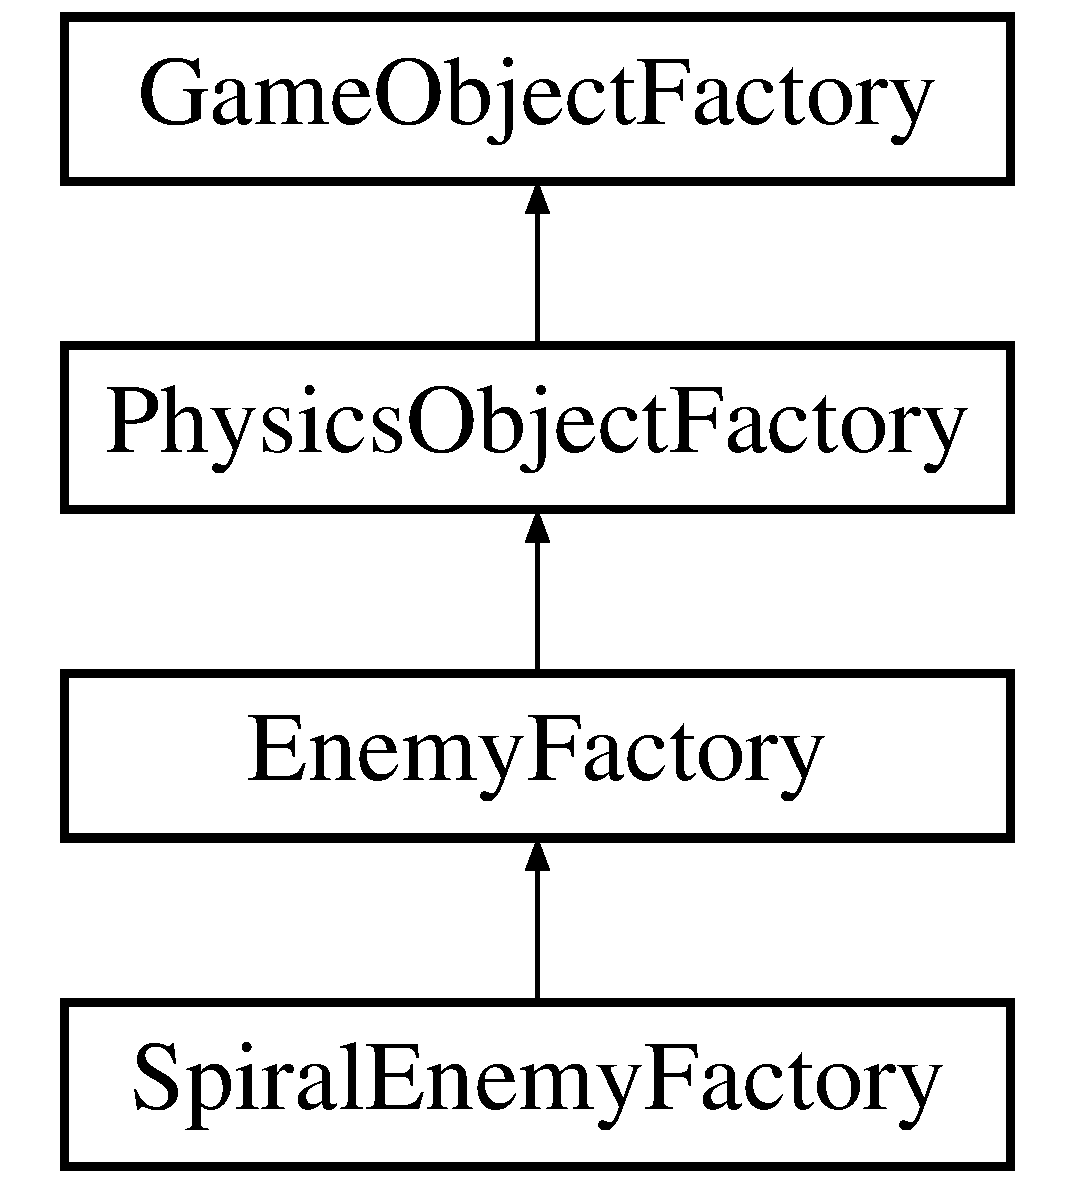
\includegraphics[height=4.000000cm]{dd/ddd/class_spiral_enemy_factory}
\end{center}
\end{figure}
\subsection*{Public Member Functions}
\begin{DoxyCompactItemize}
\item 
virtual std\+::shared\+\_\+ptr$<$ \hyperlink{class_movable_interface}{Movable\+Interface} $>$ \hyperlink{class_spiral_enemy_factory_aa05ff998b19ec4ef7ddd86ff24f70cba}{get\+Movable\+Type} (const \hyperlink{struct_game_object_data}{Game\+Object\+Data} \&data) override
\begin{DoxyCompactList}\small\item\em Pure virtual function used to assign the various Movable\+Interfaces that the Enemy\+Objects use. \end{DoxyCompactList}\item 
virtual \hyperlink{struct_game_object_data}{Game\+Object\+Data} \hyperlink{class_spiral_enemy_factory_a230709a0781c4364aa062b0bd441ec4d}{get\+Object\+Data} (const std\+::shared\+\_\+ptr$<$ \hyperlink{class_database_interface}{Database\+Interface} $>$ \&database) override
\begin{DoxyCompactList}\small\item\em used to obtain the specific \hyperlink{struct_game_object_data}{Game\+Object\+Data} defined for the current factory \end{DoxyCompactList}\end{DoxyCompactItemize}


\subsection{Detailed Description}
Generates an \hyperlink{class_enemy}{Enemy} that has a Spiral Movement Pattern. 

\subsection{Member Function Documentation}
\mbox{\Hypertarget{class_spiral_enemy_factory_aa05ff998b19ec4ef7ddd86ff24f70cba}\label{class_spiral_enemy_factory_aa05ff998b19ec4ef7ddd86ff24f70cba}} 
\index{Spiral\+Enemy\+Factory@{Spiral\+Enemy\+Factory}!get\+Movable\+Type@{get\+Movable\+Type}}
\index{get\+Movable\+Type@{get\+Movable\+Type}!Spiral\+Enemy\+Factory@{Spiral\+Enemy\+Factory}}
\subsubsection{\texorpdfstring{get\+Movable\+Type()}{getMovableType()}}
{\footnotesize\ttfamily std\+::shared\+\_\+ptr$<$ \hyperlink{class_movable_interface}{Movable\+Interface} $>$ Spiral\+Enemy\+Factory\+::get\+Movable\+Type (\begin{DoxyParamCaption}\item[{const \hyperlink{struct_game_object_data}{Game\+Object\+Data} \&}]{data }\end{DoxyParamCaption})\hspace{0.3cm}{\ttfamily [override]}, {\ttfamily [virtual]}}



Pure virtual function used to assign the various Movable\+Interfaces that the Enemy\+Objects use. 


\begin{DoxyParams}{Parameters}
{\em data} & The \hyperlink{struct_game_object_data}{Game\+Object\+Data} specific to the \hyperlink{class_enemy}{Enemy} being constructed \\
\hline
\end{DoxyParams}
\begin{DoxyReturn}{Returns}
Returns the \hyperlink{class_movable_interface}{Movable\+Interface} for the specific \hyperlink{class_enemy}{Enemy} that is being constructed 
\end{DoxyReturn}


Implements \hyperlink{class_enemy_factory_ae064082d650e676960cb84ebb60ba216}{Enemy\+Factory}.

\mbox{\Hypertarget{class_spiral_enemy_factory_a230709a0781c4364aa062b0bd441ec4d}\label{class_spiral_enemy_factory_a230709a0781c4364aa062b0bd441ec4d}} 
\index{Spiral\+Enemy\+Factory@{Spiral\+Enemy\+Factory}!get\+Object\+Data@{get\+Object\+Data}}
\index{get\+Object\+Data@{get\+Object\+Data}!Spiral\+Enemy\+Factory@{Spiral\+Enemy\+Factory}}
\subsubsection{\texorpdfstring{get\+Object\+Data()}{getObjectData()}}
{\footnotesize\ttfamily \hyperlink{struct_game_object_data}{Game\+Object\+Data} Spiral\+Enemy\+Factory\+::get\+Object\+Data (\begin{DoxyParamCaption}\item[{const std\+::shared\+\_\+ptr$<$ \hyperlink{class_database_interface}{Database\+Interface} $>$ \&}]{database }\end{DoxyParamCaption})\hspace{0.3cm}{\ttfamily [override]}, {\ttfamily [virtual]}}



used to obtain the specific \hyperlink{struct_game_object_data}{Game\+Object\+Data} defined for the current factory 


\begin{DoxyParams}{Parameters}
{\em database} & The specific \hyperlink{class_database_interface}{Database\+Interface} that contains the information about the Game\+Objects \\
\hline
\end{DoxyParams}
\begin{DoxyReturn}{Returns}
The \hyperlink{struct_game_object_data}{Game\+Object\+Data} required for the construction of the object 
\end{DoxyReturn}


Implements \hyperlink{class_physics_object_factory_aa59f52d3adc1fac676f4a8a3c2de9ba9}{Physics\+Object\+Factory}.



The documentation for this class was generated from the following files\+:\begin{DoxyCompactItemize}
\item 
C\+:/\+Users/\+Tim/\+Documents/\+Software\+Dev/\+Software\+Project/\+Project\+Files/game-\/source-\/code/\+Back\+End\+Systems/Spiral\+Enemy\+Factory.\+h\item 
C\+:/\+Users/\+Tim/\+Documents/\+Software\+Dev/\+Software\+Project/\+Project\+Files/game-\/source-\/code/\+Back\+End\+Systems/Spiral\+Enemy\+Factory.\+cpp\end{DoxyCompactItemize}

\hypertarget{class_spiral_move}{}\section{Spiral\+Move Class Reference}
\label{class_spiral_move}\index{Spiral\+Move@{Spiral\+Move}}


Used to move a \hyperlink{class_game_object}{Game\+Object} in a spiral originating from the centre of the screen.  




{\ttfamily \#include $<$Spiral\+Move.\+h$>$}

Inheritance diagram for Spiral\+Move\+:\begin{figure}[H]
\begin{center}
\leavevmode
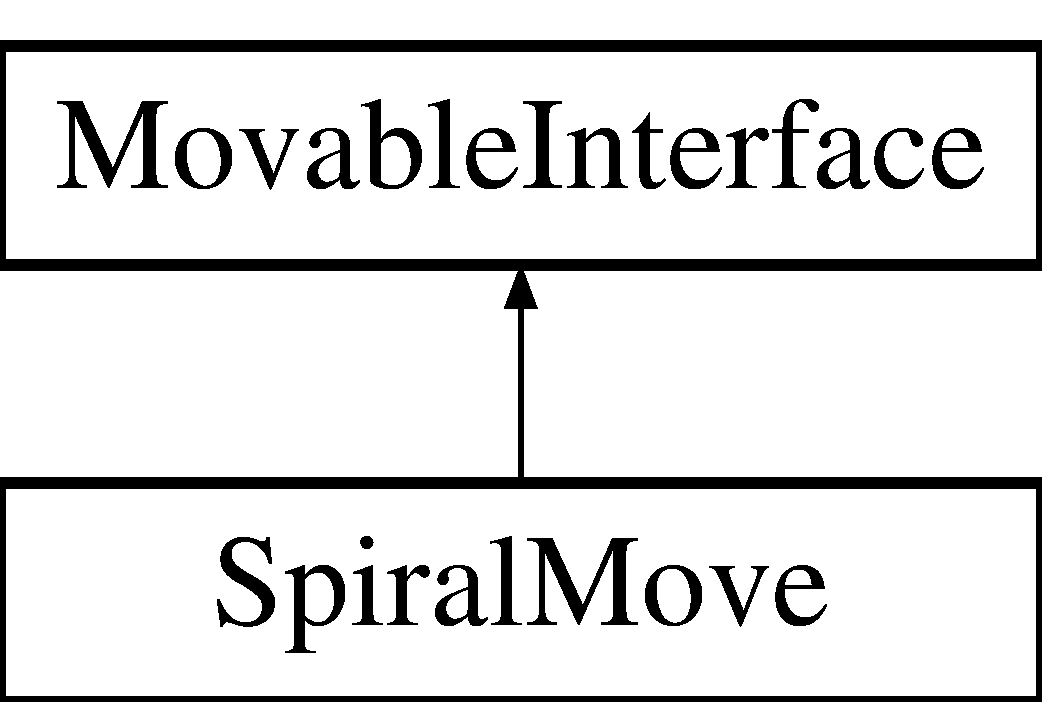
\includegraphics[height=2.000000cm]{d5/dcf/class_spiral_move}
\end{center}
\end{figure}
\subsection*{Public Member Functions}
\begin{DoxyCompactItemize}
\item 
\hyperlink{class_spiral_move_ac66bcfdc562914510243832d4762f148}{Spiral\+Move} (const double \&radial\+Speed, const double \&angular\+Speed=1)
\begin{DoxyCompactList}\small\item\em Constructs a \hyperlink{class_spiral_move}{Spiral\+Move} object with the specific speeds defined. \end{DoxyCompactList}\item 
virtual void \hyperlink{class_spiral_move_a74b22995f5f3c00c623ecaa3adb2ab8e}{Move} (\hyperlink{class_vector2_d}{Vector2D} \&current\+Position) override
\begin{DoxyCompactList}\small\item\em overrides the pure virtual function from Move\+Interface \end{DoxyCompactList}\end{DoxyCompactItemize}
\subsection*{Private Attributes}
\begin{DoxyCompactItemize}
\item 
double \hyperlink{class_spiral_move_a50cae711a780fdf56fffcb279df63f37}{\+\_\+angular\+Speed}
\end{DoxyCompactItemize}
\subsection*{Additional Inherited Members}


\subsection{Detailed Description}
Used to move a \hyperlink{class_game_object}{Game\+Object} in a spiral originating from the centre of the screen. 

\subsection{Constructor \& Destructor Documentation}
\mbox{\Hypertarget{class_spiral_move_ac66bcfdc562914510243832d4762f148}\label{class_spiral_move_ac66bcfdc562914510243832d4762f148}} 
\index{Spiral\+Move@{Spiral\+Move}!Spiral\+Move@{Spiral\+Move}}
\index{Spiral\+Move@{Spiral\+Move}!Spiral\+Move@{Spiral\+Move}}
\subsubsection{\texorpdfstring{Spiral\+Move()}{SpiralMove()}}
{\footnotesize\ttfamily Spiral\+Move\+::\+Spiral\+Move (\begin{DoxyParamCaption}\item[{const double \&}]{radial\+Speed,  }\item[{const double \&}]{angular\+Speed = {\ttfamily 1} }\end{DoxyParamCaption})}



Constructs a \hyperlink{class_spiral_move}{Spiral\+Move} object with the specific speeds defined. 


\begin{DoxyParams}{Parameters}
{\em radial\+Speed} & the speed that the object moves radially outwards from the centre is defined \\
\hline
{\em angular\+Speed} & the speed that the object rotates around the centre is defined \\
\hline
\end{DoxyParams}


\subsection{Member Function Documentation}
\mbox{\Hypertarget{class_spiral_move_a74b22995f5f3c00c623ecaa3adb2ab8e}\label{class_spiral_move_a74b22995f5f3c00c623ecaa3adb2ab8e}} 
\index{Spiral\+Move@{Spiral\+Move}!Move@{Move}}
\index{Move@{Move}!Spiral\+Move@{Spiral\+Move}}
\subsubsection{\texorpdfstring{Move()}{Move()}}
{\footnotesize\ttfamily void Spiral\+Move\+::\+Move (\begin{DoxyParamCaption}\item[{\hyperlink{class_vector2_d}{Vector2D} \&}]{current\+Position }\end{DoxyParamCaption})\hspace{0.3cm}{\ttfamily [override]}, {\ttfamily [virtual]}}



overrides the pure virtual function from Move\+Interface 


\begin{DoxyParams}{Parameters}
{\em current\+Position} & Referenced \hyperlink{class_vector2_d}{Vector2D} object for the current position that is then adjusted accordingly \\
\hline
\end{DoxyParams}


Implements \hyperlink{class_movable_interface_a899cc1c78eacbee13b906c6770e7f025}{Movable\+Interface}.



\subsection{Member Data Documentation}
\mbox{\Hypertarget{class_spiral_move_a50cae711a780fdf56fffcb279df63f37}\label{class_spiral_move_a50cae711a780fdf56fffcb279df63f37}} 
\index{Spiral\+Move@{Spiral\+Move}!\+\_\+angular\+Speed@{\+\_\+angular\+Speed}}
\index{\+\_\+angular\+Speed@{\+\_\+angular\+Speed}!Spiral\+Move@{Spiral\+Move}}
\subsubsection{\texorpdfstring{\+\_\+angular\+Speed}{\_angularSpeed}}
{\footnotesize\ttfamily double Spiral\+Move\+::\+\_\+angular\+Speed\hspace{0.3cm}{\ttfamily [private]}}

The speed that the object rotates around the centre of the screen 

The documentation for this class was generated from the following files\+:\begin{DoxyCompactItemize}
\item 
C\+:/\+Users/\+Tim/\+Documents/\+Software\+Dev/\+Software\+Project/\+Project\+Files/game-\/source-\/code/\+Front\+End\+Systems/Spiral\+Move.\+h\item 
C\+:/\+Users/\+Tim/\+Documents/\+Software\+Dev/\+Software\+Project/\+Project\+Files/game-\/source-\/code/\+Front\+End\+Systems/Spiral\+Move.\+cpp\end{DoxyCompactItemize}

\hypertarget{class_splash_scene_factory}{}\section{Splash\+Scene\+Factory Class Reference}
\label{class_splash_scene_factory}\index{Splash\+Scene\+Factory@{Splash\+Scene\+Factory}}


Creates the Splash Screen \hyperlink{class_scene}{Scene} for the game.  




{\ttfamily \#include $<$Splash\+Scene\+Factory.\+h$>$}

Inheritance diagram for Splash\+Scene\+Factory\+:\begin{figure}[H]
\begin{center}
\leavevmode
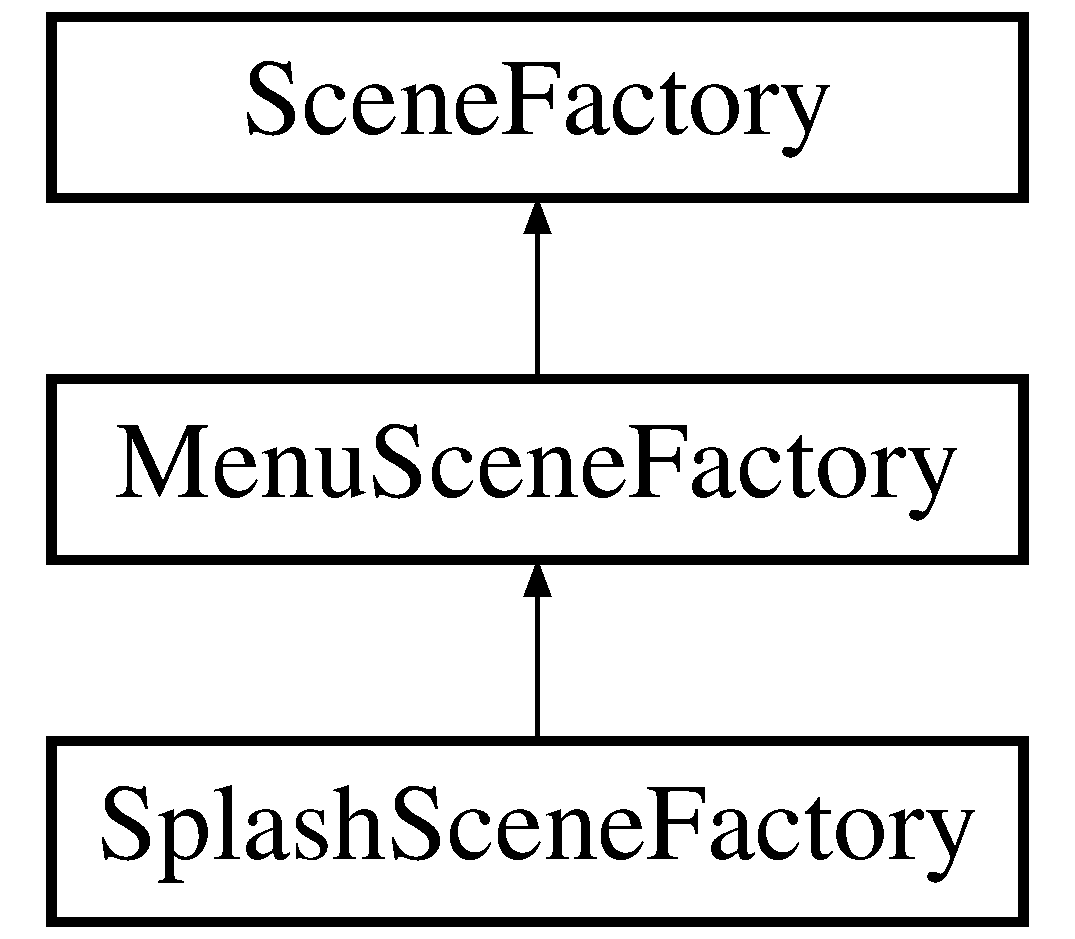
\includegraphics[height=3.000000cm]{d4/ded/class_splash_scene_factory}
\end{center}
\end{figure}
\subsection*{Protected Member Functions}
\begin{DoxyCompactItemize}
\item 
\mbox{\Hypertarget{class_splash_scene_factory_a08e3da2eb18122670b40c3520462db51}\label{class_splash_scene_factory_a08e3da2eb18122670b40c3520462db51}} 
virtual std\+::shared\+\_\+ptr$<$ \hyperlink{class_background_factory}{Background\+Factory} $>$ {\bfseries get\+Factory} () const override
\end{DoxyCompactItemize}
\subsection*{Additional Inherited Members}


\subsection{Detailed Description}
Creates the Splash Screen \hyperlink{class_scene}{Scene} for the game. 

The documentation for this class was generated from the following file\+:\begin{DoxyCompactItemize}
\item 
D\+:/\+Users/\+Tim-\/\+P\+C/\+Documents/\+Software\+\_\+\+I\+I/\+Project/\+Project\+Files/game-\/source-\/code/\+Back\+End\+Systems/Splash\+Scene\+Factory.\+h\end{DoxyCompactItemize}

\hypertarget{class_splash_screen}{}\section{Splash\+Screen Class Reference}
\label{class_splash_screen}\index{Splash\+Screen@{Splash\+Screen}}


\hyperlink{class_splash_screen}{Splash\+Screen} is used to represent a background image within the game and has the responsibility of loading the game scene and exiting the game.  




{\ttfamily \#include $<$Splash\+Screen.\+h$>$}

Inheritance diagram for Splash\+Screen\+:\begin{figure}[H]
\begin{center}
\leavevmode
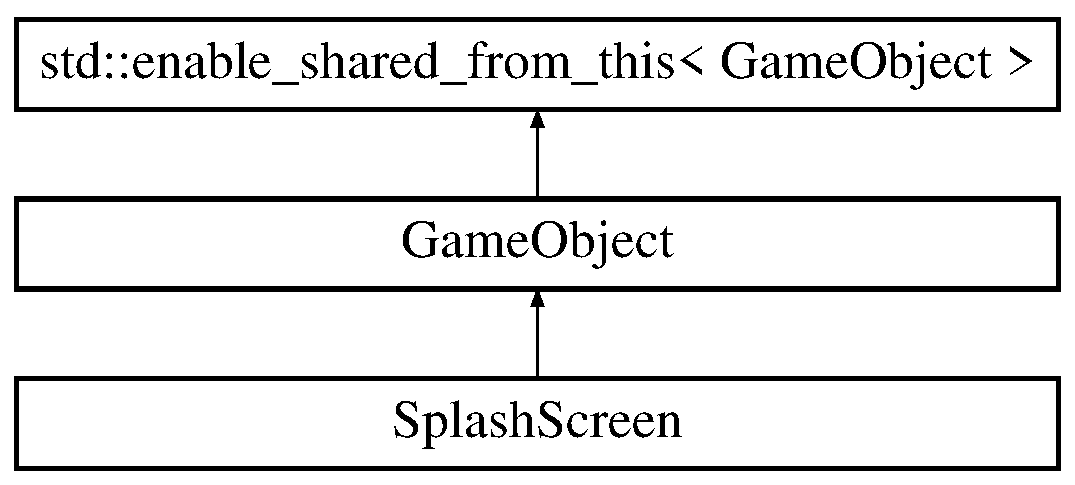
\includegraphics[height=3.000000cm]{da/d1c/class_splash_screen}
\end{center}
\end{figure}
\subsection*{Public Member Functions}
\begin{DoxyCompactItemize}
\item 
\hyperlink{class_splash_screen_afefa0db946b214828634c7f2550677e6}{Splash\+Screen} (const \hyperlink{class_game_object}{Game\+Object} \&game\+Object)
\begin{DoxyCompactList}\small\item\em The constructor for a splashscreen takes in a gameobject which is copied into the base gameobject of class to define the base parameters. \end{DoxyCompactList}\item 
\mbox{\Hypertarget{class_splash_screen_af78b8eab226a89fec389e53cbf3ed9e8}\label{class_splash_screen_af78b8eab226a89fec389e53cbf3ed9e8}} 
void \hyperlink{class_splash_screen_af78b8eab226a89fec389e53cbf3ed9e8}{Update} () override
\begin{DoxyCompactList}\small\item\em Checks for user input to identify if the Game \hyperlink{class_scene}{Scene} should be loaded/\+Restarted or if the game should exit. \end{DoxyCompactList}\end{DoxyCompactItemize}
\subsection*{Private Member Functions}
\begin{DoxyCompactItemize}
\item 
\mbox{\Hypertarget{class_splash_screen_a5d9ac6cec631b24cc947dda245e7d151}\label{class_splash_screen_a5d9ac6cec631b24cc947dda245e7d151}} 
void \hyperlink{class_splash_screen_a5d9ac6cec631b24cc947dda245e7d151}{Quit\+Game} ()
\begin{DoxyCompactList}\small\item\em Quits the game when escape is pressed. \end{DoxyCompactList}\item 
\mbox{\Hypertarget{class_splash_screen_a008328b85475bd01e326f94f20bf9217}\label{class_splash_screen_a008328b85475bd01e326f94f20bf9217}} 
void \hyperlink{class_splash_screen_a008328b85475bd01e326f94f20bf9217}{Play\+Game} ()
\begin{DoxyCompactList}\small\item\em Loads the game \hyperlink{class_scene}{Scene} when Enter is pressed. \end{DoxyCompactList}\end{DoxyCompactItemize}
\subsection*{Additional Inherited Members}


\subsection{Detailed Description}
\hyperlink{class_splash_screen}{Splash\+Screen} is used to represent a background image within the game and has the responsibility of loading the game scene and exiting the game. 

The class responsibilities of this class are should rather be seperated into a Background\+Object and a Menu\+Controller object it is currently designed incorrectly 

\subsection{Constructor \& Destructor Documentation}
\mbox{\Hypertarget{class_splash_screen_afefa0db946b214828634c7f2550677e6}\label{class_splash_screen_afefa0db946b214828634c7f2550677e6}} 
\index{Splash\+Screen@{Splash\+Screen}!Splash\+Screen@{Splash\+Screen}}
\index{Splash\+Screen@{Splash\+Screen}!Splash\+Screen@{Splash\+Screen}}
\subsubsection{\texorpdfstring{Splash\+Screen()}{SplashScreen()}}
{\footnotesize\ttfamily Splash\+Screen\+::\+Splash\+Screen (\begin{DoxyParamCaption}\item[{const \hyperlink{class_game_object}{Game\+Object} \&}]{game\+Object }\end{DoxyParamCaption})}



The constructor for a splashscreen takes in a gameobject which is copied into the base gameobject of class to define the base parameters. 


\begin{DoxyParams}{Parameters}
{\em game\+Object} & \hyperlink{class_game_object}{Game\+Object} that contains the base parameters for the current instance of the \hyperlink{class_splash_screen}{Splash\+Screen} \\
\hline
\end{DoxyParams}


The documentation for this class was generated from the following files\+:\begin{DoxyCompactItemize}
\item 
D\+:/\+Users/\+Tim-\/\+P\+C/\+Documents/\+Software\+\_\+\+I\+I/\+Project/\+Project\+Files/game-\/source-\/code/\+Front\+End\+Systems/Splash\+Screen.\+h\item 
D\+:/\+Users/\+Tim-\/\+P\+C/\+Documents/\+Software\+\_\+\+I\+I/\+Project/\+Project\+Files/game-\/source-\/code/\+Front\+End\+Systems/Splash\+Screen.\+cpp\end{DoxyCompactItemize}

\hypertarget{struct_sprite_info}{}\section{Sprite\+Info Struct Reference}
\label{struct_sprite_info}\index{Sprite\+Info@{Sprite\+Info}}


{\ttfamily \#include $<$Sprite\+Info.\+h$>$}

\subsection*{Public Attributes}
\begin{DoxyCompactItemize}
\item 
\mbox{\Hypertarget{struct_sprite_info_a0cbb7ab027f95f8b936eaaa021d51ce9}\label{struct_sprite_info_a0cbb7ab027f95f8b936eaaa021d51ce9}} 
Sprite {\bfseries sprite}
\item 
\mbox{\Hypertarget{struct_sprite_info_a29a5ebd0f1e39394af99bee4658b2b8a}\label{struct_sprite_info_a29a5ebd0f1e39394af99bee4658b2b8a}} 
Texture {\bfseries texture}
\end{DoxyCompactItemize}


\subsection{Detailed Description}
Neeeds complete Restructuring \hyperlink{struct_sprite_info}{Sprite\+Info} should be form part of the \hyperlink{class_display_manager}{Display\+Manager} and Sprite\+Data should be part of the Gameobject 

The documentation for this struct was generated from the following file\+:\begin{DoxyCompactItemize}
\item 
D\+:/\+Users/\+Tim-\/\+P\+C/\+Documents/\+Software\+\_\+\+I\+I/\+Project/\+Project\+Files/game-\/source-\/code/\+Front\+End\+Systems/Sprite\+Info.\+h\end{DoxyCompactItemize}

\hypertarget{class_string_conversions}{}\section{String\+Conversions Class Reference}
\label{class_string_conversions}\index{String\+Conversions@{String\+Conversions}}


Converts a string to the various datatypes required by the implementation.  




{\ttfamily \#include $<$String\+Conversions.\+h$>$}

\subsection*{Static Public Member Functions}
\begin{DoxyCompactItemize}
\item 
static double \hyperlink{class_string_conversions_aa48474d8bc56726261b8d7e13c4c4ab5}{string2double} (const std\+::string \&str)
\begin{DoxyCompactList}\small\item\em Convertes a string to a double. \end{DoxyCompactList}\item 
static unsigned int \hyperlink{class_string_conversions_a74a58903eb2c9971a0fe3ededbde9504}{string2uint} (const std\+::string \&str)
\begin{DoxyCompactList}\small\item\em converts a string to an unsigned integer \end{DoxyCompactList}\end{DoxyCompactItemize}


\subsection{Detailed Description}
Converts a string to the various datatypes required by the implementation. 

\subsection{Member Function Documentation}
\mbox{\Hypertarget{class_string_conversions_aa48474d8bc56726261b8d7e13c4c4ab5}\label{class_string_conversions_aa48474d8bc56726261b8d7e13c4c4ab5}} 
\index{String\+Conversions@{String\+Conversions}!string2double@{string2double}}
\index{string2double@{string2double}!String\+Conversions@{String\+Conversions}}
\subsubsection{\texorpdfstring{string2double()}{string2double()}}
{\footnotesize\ttfamily double String\+Conversions\+::string2double (\begin{DoxyParamCaption}\item[{const std\+::string \&}]{str }\end{DoxyParamCaption})\hspace{0.3cm}{\ttfamily [static]}}



Convertes a string to a double. 


\begin{DoxyParams}{Parameters}
{\em str} & the string that is converted \\
\hline
\end{DoxyParams}
\begin{DoxyReturn}{Returns}
the double that is determined from the string 
\end{DoxyReturn}
\mbox{\Hypertarget{class_string_conversions_a74a58903eb2c9971a0fe3ededbde9504}\label{class_string_conversions_a74a58903eb2c9971a0fe3ededbde9504}} 
\index{String\+Conversions@{String\+Conversions}!string2uint@{string2uint}}
\index{string2uint@{string2uint}!String\+Conversions@{String\+Conversions}}
\subsubsection{\texorpdfstring{string2uint()}{string2uint()}}
{\footnotesize\ttfamily unsigned int String\+Conversions\+::string2uint (\begin{DoxyParamCaption}\item[{const std\+::string \&}]{str }\end{DoxyParamCaption})\hspace{0.3cm}{\ttfamily [static]}}



converts a string to an unsigned integer 


\begin{DoxyParams}{Parameters}
{\em str} & the string that is converted \\
\hline
\end{DoxyParams}
\begin{DoxyReturn}{Returns}
the unsigned int that is determined from the string 
\end{DoxyReturn}


The documentation for this class was generated from the following files\+:\begin{DoxyCompactItemize}
\item 
D\+:/\+Users/\+Tim-\/\+P\+C/\+Documents/\+Software\+\_\+\+I\+I/\+Project/\+Project\+Files/game-\/source-\/code/\+Back\+End\+Systems/String\+Conversions.\+h\item 
D\+:/\+Users/\+Tim-\/\+P\+C/\+Documents/\+Software\+\_\+\+I\+I/\+Project/\+Project\+Files/game-\/source-\/code/\+Back\+End\+Systems/String\+Conversions.\+cpp\end{DoxyCompactItemize}

\hypertarget{class_update_game_object_display}{}\section{Update\+Game\+Object\+Display Class Reference}
\label{class_update_game_object_display}\index{Update\+Game\+Object\+Display@{Update\+Game\+Object\+Display}}


Updates the Sprite position and scale for each Game\+Oject.  




{\ttfamily \#include $<$Update\+Game\+Object\+Display.\+h$>$}

\subsection*{Public Member Functions}
\begin{DoxyCompactItemize}
\item 
const sf\+::\+Sprite \& \hyperlink{class_update_game_object_display_ac17a26f7563060fb9d4a0eb8959b1d29}{Determine\+Game\+Object\+Changes} (shared\+\_\+ptr$<$ \hyperlink{class_game_object}{Game\+Object} $>$ GO)
\begin{DoxyCompactList}\small\item\em Identifies and applies any changes made to a \hyperlink{class_game_object}{Game\+Object} and updates a sprite that corresponds to the changes in scale and position of that \hyperlink{class_game_object}{Game\+Object}. \end{DoxyCompactList}\item 
const unsigned int \hyperlink{class_update_game_object_display_a84972d99bd8f15ca869fc3710b836283}{get\+Hash\+Table\+Size} () const
\begin{DoxyCompactList}\small\item\em determines the current size of the hashtable made up of \hyperlink{struct_sprite_info}{Sprite\+Info} \end{DoxyCompactList}\end{DoxyCompactItemize}
\subsection*{Private Member Functions}
\begin{DoxyCompactItemize}
\item 
void \hyperlink{class_update_game_object_display_ab9405bbbabaa083cfdaefbbe84cb7cd4}{Initialise\+Sprite\+Info} (const \hyperlink{class_graphic_object}{Graphic\+Object} \&graphic\+Object)
\begin{DoxyCompactList}\small\item\em Initialises the Sprite Info that corresponds with the graphic object that is being drawn. Is only called when a \hyperlink{struct_sprite_info}{Sprite\+Info} does not exist inside of the hash table. \end{DoxyCompactList}\item 
const sf\+::\+Sprite \& \hyperlink{class_update_game_object_display_a05f0b24dfb3e2206b0d363dbc5127139}{Update\+Sprite\+Properties} (const \hyperlink{class_vector2_d}{Vector2D} \&position, const \hyperlink{structxy_vector}{xy\+Vector} \&scale, const string \&current\+Object\+Key)
\begin{DoxyCompactList}\small\item\em Updates the sprite properties according to the information from the corresponding \hyperlink{class_game_object}{Game\+Object}. \end{DoxyCompactList}\item 
bool \hyperlink{class_update_game_object_display_a10502ed4d422e5bab6b5f3591d392c55}{Check\+If\+Sprite\+Info\+Exists} (const \hyperlink{class_graphic_object}{Graphic\+Object} \&corresponding\+Graphic)
\begin{DoxyCompactList}\small\item\em Checks if the \hyperlink{struct_sprite_info}{Sprite\+Info} that corresponds to a particular graphic object has already been generated and is being stored in the hash table. \end{DoxyCompactList}\end{DoxyCompactItemize}
\subsection*{Private Attributes}
\begin{DoxyCompactItemize}
\item 
std\+::unordered\+\_\+map$<$ std\+::string, std\+::shared\+\_\+ptr$<$ \hyperlink{struct_sprite_info}{Sprite\+Info} $>$ $>$ \hyperlink{class_update_game_object_display_a51ae3f07958294b737885c9a0bd86153}{\+\_\+sprite\+Info\+Table}
\end{DoxyCompactItemize}


\subsection{Detailed Description}
Updates the Sprite position and scale for each Game\+Oject. 

contains a hash table that stores the individual sprites and corresponding textures for the specific key provided within the \hyperlink{class_graphic_object}{Graphic\+Object} composition of the \hyperlink{class_game_object}{Game\+Object}. Updates the screen position and scale of the sprite for each game object provided. If the sprite and texture do not exist inside of the hash table it is created and added into it. 

\subsection{Member Function Documentation}
\mbox{\Hypertarget{class_update_game_object_display_a10502ed4d422e5bab6b5f3591d392c55}\label{class_update_game_object_display_a10502ed4d422e5bab6b5f3591d392c55}} 
\index{Update\+Game\+Object\+Display@{Update\+Game\+Object\+Display}!Check\+If\+Sprite\+Info\+Exists@{Check\+If\+Sprite\+Info\+Exists}}
\index{Check\+If\+Sprite\+Info\+Exists@{Check\+If\+Sprite\+Info\+Exists}!Update\+Game\+Object\+Display@{Update\+Game\+Object\+Display}}
\subsubsection{\texorpdfstring{Check\+If\+Sprite\+Info\+Exists()}{CheckIfSpriteInfoExists()}}
{\footnotesize\ttfamily bool Update\+Game\+Object\+Display\+::\+Check\+If\+Sprite\+Info\+Exists (\begin{DoxyParamCaption}\item[{const \hyperlink{class_graphic_object}{Graphic\+Object} \&}]{corresponding\+Graphic }\end{DoxyParamCaption})\hspace{0.3cm}{\ttfamily [private]}}



Checks if the \hyperlink{struct_sprite_info}{Sprite\+Info} that corresponds to a particular graphic object has already been generated and is being stored in the hash table. 


\begin{DoxyParams}{Parameters}
{\em corresponding\+Graphic} & The Corresponding \hyperlink{class_graphic_object}{Graphic\+Object} to the \hyperlink{struct_sprite_info}{Sprite\+Info} in the table \\
\hline
\end{DoxyParams}
\begin{DoxyReturn}{Returns}
returns true if the \hyperlink{struct_sprite_info}{Sprite\+Info} does Exist
\end{DoxyReturn}
Determines whether the \hyperlink{struct_sprite_info}{Sprite\+Info} object that corresponds to the key obtained from the graphic object exists. Uses std\+::find to check for the object and returns a true if the iterator returned is not equal to the end of the hash table \mbox{\Hypertarget{class_update_game_object_display_ac17a26f7563060fb9d4a0eb8959b1d29}\label{class_update_game_object_display_ac17a26f7563060fb9d4a0eb8959b1d29}} 
\index{Update\+Game\+Object\+Display@{Update\+Game\+Object\+Display}!Determine\+Game\+Object\+Changes@{Determine\+Game\+Object\+Changes}}
\index{Determine\+Game\+Object\+Changes@{Determine\+Game\+Object\+Changes}!Update\+Game\+Object\+Display@{Update\+Game\+Object\+Display}}
\subsubsection{\texorpdfstring{Determine\+Game\+Object\+Changes()}{DetermineGameObjectChanges()}}
{\footnotesize\ttfamily const sf\+::\+Sprite \& Update\+Game\+Object\+Display\+::\+Determine\+Game\+Object\+Changes (\begin{DoxyParamCaption}\item[{shared\+\_\+ptr$<$ \hyperlink{class_game_object}{Game\+Object} $>$}]{GO }\end{DoxyParamCaption})}



Identifies and applies any changes made to a \hyperlink{class_game_object}{Game\+Object} and updates a sprite that corresponds to the changes in scale and position of that \hyperlink{class_game_object}{Game\+Object}. 


\begin{DoxyParams}{Parameters}
{\em GO} & an std\+::shared\+\_\+ptr to the \hyperlink{class_game_object}{Game\+Object} that is being checked for changes\\
\hline
\end{DoxyParams}
Initially Identifies if the \hyperlink{class_game_object}{Game\+Object}\textquotesingle{}s corresponding sprite has been drawn before. If it does not exist a texture is created according to the information stored inside of the \hyperlink{class_graphic_object}{Graphic\+Object} Composition and the sprite is setup accordingly. After which the sprite is updated to the corresponding scale and position of the \hyperlink{class_game_object}{Game\+Object} \mbox{\Hypertarget{class_update_game_object_display_a84972d99bd8f15ca869fc3710b836283}\label{class_update_game_object_display_a84972d99bd8f15ca869fc3710b836283}} 
\index{Update\+Game\+Object\+Display@{Update\+Game\+Object\+Display}!get\+Hash\+Table\+Size@{get\+Hash\+Table\+Size}}
\index{get\+Hash\+Table\+Size@{get\+Hash\+Table\+Size}!Update\+Game\+Object\+Display@{Update\+Game\+Object\+Display}}
\subsubsection{\texorpdfstring{get\+Hash\+Table\+Size()}{getHashTableSize()}}
{\footnotesize\ttfamily const unsigned int Update\+Game\+Object\+Display\+::get\+Hash\+Table\+Size (\begin{DoxyParamCaption}{ }\end{DoxyParamCaption}) const\hspace{0.3cm}{\ttfamily [inline]}}



determines the current size of the hashtable made up of \hyperlink{struct_sprite_info}{Sprite\+Info} 

\begin{DoxyReturn}{Returns}
Returns the size of the hashtable used to store the various \hyperlink{struct_sprite_info}{Sprite\+Info} Objects 
\end{DoxyReturn}
\mbox{\Hypertarget{class_update_game_object_display_ab9405bbbabaa083cfdaefbbe84cb7cd4}\label{class_update_game_object_display_ab9405bbbabaa083cfdaefbbe84cb7cd4}} 
\index{Update\+Game\+Object\+Display@{Update\+Game\+Object\+Display}!Initialise\+Sprite\+Info@{Initialise\+Sprite\+Info}}
\index{Initialise\+Sprite\+Info@{Initialise\+Sprite\+Info}!Update\+Game\+Object\+Display@{Update\+Game\+Object\+Display}}
\subsubsection{\texorpdfstring{Initialise\+Sprite\+Info()}{InitialiseSpriteInfo()}}
{\footnotesize\ttfamily void Update\+Game\+Object\+Display\+::\+Initialise\+Sprite\+Info (\begin{DoxyParamCaption}\item[{const \hyperlink{class_graphic_object}{Graphic\+Object} \&}]{graphic\+Object }\end{DoxyParamCaption})\hspace{0.3cm}{\ttfamily [private]}}



Initialises the Sprite Info that corresponds with the graphic object that is being drawn. Is only called when a \hyperlink{struct_sprite_info}{Sprite\+Info} does not exist inside of the hash table. 


\begin{DoxyParams}{Parameters}
{\em graphic\+Object} & The \hyperlink{class_graphic_object}{Graphic\+Object} which contains the texture location for the corresponding \hyperlink{class_game_object}{Game\+Object} \\
\hline
\end{DoxyParams}
\mbox{\Hypertarget{class_update_game_object_display_a05f0b24dfb3e2206b0d363dbc5127139}\label{class_update_game_object_display_a05f0b24dfb3e2206b0d363dbc5127139}} 
\index{Update\+Game\+Object\+Display@{Update\+Game\+Object\+Display}!Update\+Sprite\+Properties@{Update\+Sprite\+Properties}}
\index{Update\+Sprite\+Properties@{Update\+Sprite\+Properties}!Update\+Game\+Object\+Display@{Update\+Game\+Object\+Display}}
\subsubsection{\texorpdfstring{Update\+Sprite\+Properties()}{UpdateSpriteProperties()}}
{\footnotesize\ttfamily const sf\+::\+Sprite \& Update\+Game\+Object\+Display\+::\+Update\+Sprite\+Properties (\begin{DoxyParamCaption}\item[{const \hyperlink{class_vector2_d}{Vector2D} \&}]{position,  }\item[{const \hyperlink{structxy_vector}{xy\+Vector} \&}]{scale,  }\item[{const string \&}]{current\+Object\+Key }\end{DoxyParamCaption})\hspace{0.3cm}{\ttfamily [private]}}



Updates the sprite properties according to the information from the corresponding \hyperlink{class_game_object}{Game\+Object}. 


\begin{DoxyParams}{Parameters}
{\em position} & The updated game\+Position of the \hyperlink{class_game_object}{Game\+Object} \\
\hline
{\em scale} & The updated scale of the \hyperlink{class_game_object}{Game\+Object} \\
\hline
\end{DoxyParams}
\begin{DoxyReturn}{Returns}
Returns the sprite object that has been updated with a new position and scale
\end{DoxyReturn}
Updates the position of the sprite ,retrieved from the hash table, to the corresponding screen position by converting the Game\+Oject\textquotesingle{}s game position to the corresponding screen position and then assigns the scale of the object to sprite 

\subsection{Member Data Documentation}
\mbox{\Hypertarget{class_update_game_object_display_a51ae3f07958294b737885c9a0bd86153}\label{class_update_game_object_display_a51ae3f07958294b737885c9a0bd86153}} 
\index{Update\+Game\+Object\+Display@{Update\+Game\+Object\+Display}!\+\_\+sprite\+Info\+Table@{\+\_\+sprite\+Info\+Table}}
\index{\+\_\+sprite\+Info\+Table@{\+\_\+sprite\+Info\+Table}!Update\+Game\+Object\+Display@{Update\+Game\+Object\+Display}}
\subsubsection{\texorpdfstring{\+\_\+sprite\+Info\+Table}{\_spriteInfoTable}}
{\footnotesize\ttfamily std\+::unordered\+\_\+map$<$std\+::string, std\+::shared\+\_\+ptr$<$\hyperlink{struct_sprite_info}{Sprite\+Info}$>$ $>$ Update\+Game\+Object\+Display\+::\+\_\+sprite\+Info\+Table\hspace{0.3cm}{\ttfamily [private]}}

The hashtable used to store the \hyperlink{struct_sprite_info}{Sprite\+Info}\textquotesingle{}s for each game\+Object 

The documentation for this class was generated from the following files\+:\begin{DoxyCompactItemize}
\item 
D\+:/\+Users/\+Tim-\/\+P\+C/\+Documents/\+Software\+\_\+\+I\+I/\+Project/\+Project\+Files/game-\/source-\/code/\+Back\+End\+Systems/Update\+Game\+Object\+Display.\+h\item 
D\+:/\+Users/\+Tim-\/\+P\+C/\+Documents/\+Software\+\_\+\+I\+I/\+Project/\+Project\+Files/game-\/source-\/code/\+Back\+End\+Systems/Update\+Game\+Object\+Diplay.\+cpp\end{DoxyCompactItemize}

\hypertarget{class_vector2_d}{}\section{Vector2D Class Reference}
\label{class_vector2_d}\index{Vector2D@{Vector2D}}


Defines the base mathematical element used, the \hyperlink{class_vector2_d}{Vector2D} element. Contains structs of two self-\/contained vector types, the \hyperlink{structxy_vector}{xy\+Vector} and the \hyperlink{structrt_vector}{rt\+Vector}. Defines the associated creation of the objects, and the logical operator overload associated with vector mathematics. The tigonometric mathematical vector relationships are based on radians.  




{\ttfamily \#include $<$Vector2\+D.\+h$>$}

\subsection*{Public Member Functions}
\begin{DoxyCompactItemize}
\item 
\hyperlink{class_vector2_d_a98e9997ebb7a629f4db52397d4e0d653}{Vector2D} ()
\begin{DoxyCompactList}\small\item\em Default constructor for the \hyperlink{class_vector2_d}{Vector2D} class. Assigns the static origin of the \hyperlink{class_vector2_d}{Vector2D} class to this \hyperlink{class_vector2_d}{Vector2D} object. \end{DoxyCompactList}\item 
\hyperlink{class_vector2_d_a0c1db105a3d49bde5056cc19b04f18c2}{Vector2D} (double val1, double val2, const Vector\+Type \&vectype=Vector\+Type\+::xy)
\begin{DoxyCompactList}\small\item\em Constructor for the \hyperlink{class_vector2_d}{Vector2D} class by two double scalar parameters, and the vector input type. Constructs the \hyperlink{class_vector2_d}{Vector2D} object appropriately based from the vectype parameter. \end{DoxyCompactList}\item 
\hyperlink{class_vector2_d_ab3aae16cfdb6eab642f832d82de2ac5c}{Vector2D} (const \hyperlink{structxy_vector}{xy\+Vector} vec)
\begin{DoxyCompactList}\small\item\em Constructor for the \hyperlink{class_vector2_d}{Vector2D} class directly from a \hyperlink{structxy_vector}{xy\+Vector} struct. \end{DoxyCompactList}\item 
\hyperlink{class_vector2_d_a3253f7c676f03f9d460d6b473934a1ff}{Vector2D} (const \hyperlink{structrt_vector}{rt\+Vector} vec)
\begin{DoxyCompactList}\small\item\em Constructor for the \hyperlink{class_vector2_d}{Vector2D} class directly from a \hyperlink{structrt_vector}{rt\+Vector} struct. \end{DoxyCompactList}\item 
\hyperlink{class_vector2_d_a658f4dd52408392ab5ad5fb36112a5c8}{Vector2D} (const \hyperlink{class_vector2_d}{Vector2D} \&rhs)
\begin{DoxyCompactList}\small\item\em Copy constructor for the \hyperlink{class_vector2_d}{Vector2D} class. \end{DoxyCompactList}\item 
\hyperlink{structxy_vector}{xy\+Vector} \hyperlink{class_vector2_d_a4bc415751c246ae44727ef4f6b80d80c}{get\+X\+Y\+Vector} () const
\begin{DoxyCompactList}\small\item\em Allows the \hyperlink{structxy_vector}{xy\+Vector} struct value of the \hyperlink{class_vector2_d}{Vector2D} object to be querried. Fundamentally the cartesian representation of the \hyperlink{class_vector2_d}{Vector2D} position. \end{DoxyCompactList}\item 
\hyperlink{structrt_vector}{rt\+Vector} \hyperlink{class_vector2_d_a2760dd54ac65996966d1b9077cbecb06}{get\+R\+T\+Vector} () const
\begin{DoxyCompactList}\small\item\em Allows the \hyperlink{structrt_vector}{rt\+Vector} struct value of the \hyperlink{class_vector2_d}{Vector2D} object to be querried. Fundamentally the polar representation of the \hyperlink{class_vector2_d}{Vector2D} position. \end{DoxyCompactList}\item 
\hyperlink{class_vector2_d}{Vector2D} \& \hyperlink{class_vector2_d_abfa56cdcf167527e7c5efd54c4c1bffe}{operator=} (const \hyperlink{class_vector2_d}{Vector2D} \&rhs)
\begin{DoxyCompactList}\small\item\em this\+Vector2D = rhs\+Vector2D\+: The assignment operator overload defined for the \hyperlink{class_vector2_d}{Vector2D} class. \end{DoxyCompactList}\item 
bool \hyperlink{class_vector2_d_a41f425fcd08fb82c7e72e132fb51136f}{operator==} (const \hyperlink{class_vector2_d}{Vector2D} \&rhs) const
\begin{DoxyCompactList}\small\item\em this\+Vector2D == rhs\+Vector2D\+: The equivalancy operator overload defined for the \hyperlink{class_vector2_d}{Vector2D} class. \end{DoxyCompactList}\item 
\hyperlink{class_vector2_d}{Vector2D} \hyperlink{class_vector2_d_a142a352f6cb2406fee15d153a275439c}{operator+} (const \hyperlink{class_vector2_d}{Vector2D} \&rhs) const
\begin{DoxyCompactList}\small\item\em new\+Vector2D = this\+Vector2D + rhs\+Vector2D\+: The vector addition and create operator overload defined for the \hyperlink{class_vector2_d}{Vector2D} class. \end{DoxyCompactList}\item 
\hyperlink{class_vector2_d}{Vector2D} \hyperlink{class_vector2_d_a803ee7e8cc2bfac23eb9e3aeebd5be3f}{operator-\/} (const \hyperlink{class_vector2_d}{Vector2D} \&rhs) const
\begin{DoxyCompactList}\small\item\em new\+Vector2D = this\+Vector2D -\/ rhs\+Vector2D\+: The vector subtraction and create operator overload defined for the \hyperlink{class_vector2_d}{Vector2D} class. \end{DoxyCompactList}\item 
\hyperlink{class_vector2_d}{Vector2D} \hyperlink{class_vector2_d_a257aa1ca3260a4cacaa1171f67bf7910}{operator$\ast$} (const \hyperlink{class_vector2_d}{Vector2D} \&rhs) const
\begin{DoxyCompactList}\small\item\em new\+Vector2D = this\+Vector2D $\ast$ rhs\+Vector2D\+: The vector multiplication and create operator overload defined for the \hyperlink{class_vector2_d}{Vector2D} class. \end{DoxyCompactList}\item 
\hyperlink{class_vector2_d}{Vector2D} \hyperlink{class_vector2_d_a7ade542889c8e483b5cc536b2bf4f053}{operator$\ast$} (const double \&scalar) const
\begin{DoxyCompactList}\small\item\em new\+Vector2D = this\+Vector2D $\ast$ scalar\+: The scalar multiplication and create operator overload defined for the \hyperlink{class_vector2_d}{Vector2D} class. \end{DoxyCompactList}\item 
\hyperlink{class_vector2_d}{Vector2D} \hyperlink{class_vector2_d_adc10dc721432ed17e94602640bb24346}{operator/} (const double \&scalar) const
\begin{DoxyCompactList}\small\item\em new\+Vector2D = this\+Vector2D / scalar\+: The scalar division and create operator overload defined for the \hyperlink{class_vector2_d}{Vector2D} class. \end{DoxyCompactList}\item 
\hyperlink{class_vector2_d}{Vector2D} \& \hyperlink{class_vector2_d_affc6e2a6034a4c4249a3e8b17f633069}{operator+=} (const \hyperlink{class_vector2_d}{Vector2D} \&rhs)
\begin{DoxyCompactList}\small\item\em this\+Vector2d = this\+Vector2D + rhs\+Vector2D\+: The vector addition and assignment operator overload defined for the \hyperlink{class_vector2_d}{Vector2D} class. \end{DoxyCompactList}\item 
\hyperlink{class_vector2_d}{Vector2D} \& \hyperlink{class_vector2_d_a16532303ee3e0a340f0515c1f0675fbd}{operator-\/=} (const \hyperlink{class_vector2_d}{Vector2D} \&rhs)
\begin{DoxyCompactList}\small\item\em this\+Vector2D = this\+Vector2D -\/ rhs\+Vector2D\+: The vector subtraction and assignment operator overload defined for the \hyperlink{class_vector2_d}{Vector2D} class. \end{DoxyCompactList}\item 
\hyperlink{class_vector2_d}{Vector2D} \& \hyperlink{class_vector2_d_a7fe58ba3258641c02c7ea4499d42a089}{operator$\ast$=} (const \hyperlink{class_vector2_d}{Vector2D} \&rhs)
\begin{DoxyCompactList}\small\item\em this\+Vector2D = this\+Vector2D $\ast$ rhs\+Vector2D\+: The vector multiplication and assignment operator overload defined for the \hyperlink{class_vector2_d}{Vector2D} class. \end{DoxyCompactList}\item 
\hyperlink{class_vector2_d}{Vector2D} \& \hyperlink{class_vector2_d_abd5d60f6e25137acab01b1d82da6819a}{operator$\ast$=} (const double scale)
\begin{DoxyCompactList}\small\item\em this\+Vector2D = this\+Vector2D $\ast$ scalar\+: The scalar multiplication and assignment operator overload defined for the \hyperlink{class_vector2_d}{Vector2D} class. \end{DoxyCompactList}\item 
\hyperlink{class_vector2_d}{Vector2D} \& \hyperlink{class_vector2_d_a72a388dec12b808190830a35be86a1f7}{operator/=} (const double scale)
\begin{DoxyCompactList}\small\item\em this\+Vector2D = this\+Vector2D / scalar\+: The scalar division and assignment operator overload defined for the \hyperlink{class_vector2_d}{Vector2D} class. \end{DoxyCompactList}\item 
\hyperlink{class_vector2_d}{Vector2D} \hyperlink{class_vector2_d_a79cfa577c38cb866d088166d6729a47d}{normalize} () const
\begin{DoxyCompactList}\small\item\em Normalize function of a \hyperlink{class_vector2_d}{Vector2D} object. Normalises the \hyperlink{class_vector2_d}{Vector2D} object, to a unirary magnitude/radius, creates a new \hyperlink{class_vector2_d}{Vector2D} objectfor the returned result. This \hyperlink{class_vector2_d}{Vector2D} object remains costant under query. \end{DoxyCompactList}\end{DoxyCompactItemize}
\subsection*{Static Public Member Functions}
\begin{DoxyCompactItemize}
\item 
static double \hyperlink{class_vector2_d_a73d35a880a2f3d262b14ac8aaf5914db}{magnitude} (const \hyperlink{class_vector2_d}{Vector2D} \&lhs)
\begin{DoxyCompactList}\small\item\em Static function that calculates the vector magnitude of a \hyperlink{class_vector2_d}{Vector2D} object. Uses the origin as a comparative mathematical reference. \end{DoxyCompactList}\item 
static double \hyperlink{class_vector2_d_ac7b3cebbfa7c84c9750c30a6c030ffa8}{magnitude} (const \hyperlink{class_vector2_d}{Vector2D} \&lhs, const \hyperlink{class_vector2_d}{Vector2D} \&rhs)
\begin{DoxyCompactList}\small\item\em Static function that calculates the relative vector magnitude between two \hyperlink{class_vector2_d}{Vector2D} objects. \end{DoxyCompactList}\end{DoxyCompactItemize}
\subsection*{Static Public Attributes}
\begin{DoxyCompactItemize}
\item 
\mbox{\Hypertarget{class_vector2_d_aa7a23308562639dc04b9fe30b2e30008}\label{class_vector2_d_aa7a23308562639dc04b9fe30b2e30008}} 
static \hyperlink{class_vector2_d}{Vector2D} {\bfseries origin} \{0,0\}
\item 
\mbox{\Hypertarget{class_vector2_d_aa48eacf081c0ffd578ff0687bd261580}\label{class_vector2_d_aa48eacf081c0ffd578ff0687bd261580}} 
static \hyperlink{class_vector2_d}{Vector2D} {\bfseries right} \{1, 0\}
\item 
\mbox{\Hypertarget{class_vector2_d_a9de8398e8d132c017571a911bf20d242}\label{class_vector2_d_a9de8398e8d132c017571a911bf20d242}} 
static \hyperlink{class_vector2_d}{Vector2D} {\bfseries left} \{-\/1, 0\}
\item 
\mbox{\Hypertarget{class_vector2_d_a5ea1302008e7f6827a1153cd3d5f3ef7}\label{class_vector2_d_a5ea1302008e7f6827a1153cd3d5f3ef7}} 
static \hyperlink{class_vector2_d}{Vector2D} {\bfseries up} \{0, 1\}
\item 
\mbox{\Hypertarget{class_vector2_d_aadd75c5ef76f3f4071c6fe1a2dc27c7b}\label{class_vector2_d_aadd75c5ef76f3f4071c6fe1a2dc27c7b}} 
static \hyperlink{class_vector2_d}{Vector2D} {\bfseries down} \{0, -\/1\}
\end{DoxyCompactItemize}
\subsection*{Private Member Functions}
\begin{DoxyCompactItemize}
\item 
\mbox{\Hypertarget{class_vector2_d_a86eb002af3d4ce9ee892691165577bd9}\label{class_vector2_d_a86eb002af3d4ce9ee892691165577bd9}} 
void \hyperlink{class_vector2_d_a86eb002af3d4ce9ee892691165577bd9}{radius} ()
\begin{DoxyCompactList}\small\item\em Private function to calculate the radius from the \hyperlink{structxy_vector}{xy\+Vector} struct, to be privately stored in the \hyperlink{structrt_vector}{rt\+Vector} struct. \end{DoxyCompactList}\item 
\mbox{\Hypertarget{class_vector2_d_a77801c0448846bc99cea64b232e262ed}\label{class_vector2_d_a77801c0448846bc99cea64b232e262ed}} 
void \hyperlink{class_vector2_d_a77801c0448846bc99cea64b232e262ed}{theta} ()
\begin{DoxyCompactList}\small\item\em Private function to calculate the theta/angle from the \hyperlink{structxy_vector}{xy\+Vector} struct, to be privately stored in the \hyperlink{structrt_vector}{rt\+Vector} struct. \end{DoxyCompactList}\item 
\mbox{\Hypertarget{class_vector2_d_a2aa1adc699bfc5a490875d26c1e6da04}\label{class_vector2_d_a2aa1adc699bfc5a490875d26c1e6da04}} 
void \hyperlink{class_vector2_d_a2aa1adc699bfc5a490875d26c1e6da04}{x\+Val} ()
\begin{DoxyCompactList}\small\item\em Private function to calculate the x-\/cartesian value from the \hyperlink{structrt_vector}{rt\+Vector} struct, to be privately stored in the \hyperlink{structxy_vector}{xy\+Vector} struct. \end{DoxyCompactList}\item 
\mbox{\Hypertarget{class_vector2_d_ab202ce3f9065cdbf5d981b0f34c66feb}\label{class_vector2_d_ab202ce3f9065cdbf5d981b0f34c66feb}} 
void \hyperlink{class_vector2_d_ab202ce3f9065cdbf5d981b0f34c66feb}{y\+Val} ()
\begin{DoxyCompactList}\small\item\em Private function to calculate the y-\/cartesian value from the \hyperlink{structrt_vector}{rt\+Vector} struct, to be privately stored in the \hyperlink{structxy_vector}{xy\+Vector} struct. \end{DoxyCompactList}\end{DoxyCompactItemize}
\subsection*{Private Attributes}
\begin{DoxyCompactItemize}
\item 
\mbox{\Hypertarget{class_vector2_d_a151b8b70d16a3bf4544af58c2a721242}\label{class_vector2_d_a151b8b70d16a3bf4544af58c2a721242}} 
\hyperlink{structxy_vector}{xy\+Vector} {\bfseries \+\_\+xyvec}
\item 
\mbox{\Hypertarget{class_vector2_d_a97b229bece3801330df9ef710d0296e9}\label{class_vector2_d_a97b229bece3801330df9ef710d0296e9}} 
\hyperlink{structrt_vector}{rt\+Vector} {\bfseries \+\_\+rtvec}
\end{DoxyCompactItemize}
\subsection*{Static Private Attributes}
\begin{DoxyCompactItemize}
\item 
\mbox{\Hypertarget{class_vector2_d_a50a94297b6c05c07ee29900a438492a9}\label{class_vector2_d_a50a94297b6c05c07ee29900a438492a9}} 
static double {\bfseries magnitude\+\_\+tolerance} = 0.\+000000001
\end{DoxyCompactItemize}


\subsection{Detailed Description}
Defines the base mathematical element used, the \hyperlink{class_vector2_d}{Vector2D} element. Contains structs of two self-\/contained vector types, the \hyperlink{structxy_vector}{xy\+Vector} and the \hyperlink{structrt_vector}{rt\+Vector}. Defines the associated creation of the objects, and the logical operator overload associated with vector mathematics. The tigonometric mathematical vector relationships are based on radians. 

\subsection{Constructor \& Destructor Documentation}
\mbox{\Hypertarget{class_vector2_d_a98e9997ebb7a629f4db52397d4e0d653}\label{class_vector2_d_a98e9997ebb7a629f4db52397d4e0d653}} 
\index{Vector2D@{Vector2D}!Vector2D@{Vector2D}}
\index{Vector2D@{Vector2D}!Vector2D@{Vector2D}}
\subsubsection{\texorpdfstring{Vector2\+D()}{Vector2D()}\hspace{0.1cm}{\footnotesize\ttfamily [1/5]}}
{\footnotesize\ttfamily Vector2\+D\+::\+Vector2D (\begin{DoxyParamCaption}{ }\end{DoxyParamCaption})}



Default constructor for the \hyperlink{class_vector2_d}{Vector2D} class. Assigns the static origin of the \hyperlink{class_vector2_d}{Vector2D} class to this \hyperlink{class_vector2_d}{Vector2D} object. 

\begin{DoxyReturn}{Returns}
\hyperlink{class_vector2_d}{Vector2D} by value. 
\end{DoxyReturn}
\mbox{\Hypertarget{class_vector2_d_a0c1db105a3d49bde5056cc19b04f18c2}\label{class_vector2_d_a0c1db105a3d49bde5056cc19b04f18c2}} 
\index{Vector2D@{Vector2D}!Vector2D@{Vector2D}}
\index{Vector2D@{Vector2D}!Vector2D@{Vector2D}}
\subsubsection{\texorpdfstring{Vector2\+D()}{Vector2D()}\hspace{0.1cm}{\footnotesize\ttfamily [2/5]}}
{\footnotesize\ttfamily Vector2\+D\+::\+Vector2D (\begin{DoxyParamCaption}\item[{double}]{val1,  }\item[{double}]{val2,  }\item[{const Vector\+Type \&}]{vectype = {\ttfamily VectorType\+:\+:xy} }\end{DoxyParamCaption})}



Constructor for the \hyperlink{class_vector2_d}{Vector2D} class by two double scalar parameters, and the vector input type. Constructs the \hyperlink{class_vector2_d}{Vector2D} object appropriately based from the vectype parameter. 


\begin{DoxyParams}{Parameters}
{\em val1} & either as x value of cartesian input or radius value of polar input. \\
\hline
{\em val2} & either as y value of cartesian input or theta value of polar input. \\
\hline
{\em vectype} & of the parameters val1 and val2. Default is Vector\+Type\+::xy. \\
\hline
\end{DoxyParams}
\begin{DoxyReturn}{Returns}
\hyperlink{class_vector2_d}{Vector2D} by value. 
\end{DoxyReturn}
\mbox{\Hypertarget{class_vector2_d_ab3aae16cfdb6eab642f832d82de2ac5c}\label{class_vector2_d_ab3aae16cfdb6eab642f832d82de2ac5c}} 
\index{Vector2D@{Vector2D}!Vector2D@{Vector2D}}
\index{Vector2D@{Vector2D}!Vector2D@{Vector2D}}
\subsubsection{\texorpdfstring{Vector2\+D()}{Vector2D()}\hspace{0.1cm}{\footnotesize\ttfamily [3/5]}}
{\footnotesize\ttfamily Vector2\+D\+::\+Vector2D (\begin{DoxyParamCaption}\item[{const \hyperlink{structxy_vector}{xy\+Vector}}]{vec }\end{DoxyParamCaption})}



Constructor for the \hyperlink{class_vector2_d}{Vector2D} class directly from a \hyperlink{structxy_vector}{xy\+Vector} struct. 


\begin{DoxyParams}{Parameters}
{\em vec} & The \hyperlink{structxy_vector}{xy\+Vector} struct used for the \hyperlink{class_vector2_d}{Vector2D} object construction. Used by constant value. \\
\hline
\end{DoxyParams}
\begin{DoxyReturn}{Returns}
\hyperlink{class_vector2_d}{Vector2D} by value. 
\end{DoxyReturn}
\mbox{\Hypertarget{class_vector2_d_a3253f7c676f03f9d460d6b473934a1ff}\label{class_vector2_d_a3253f7c676f03f9d460d6b473934a1ff}} 
\index{Vector2D@{Vector2D}!Vector2D@{Vector2D}}
\index{Vector2D@{Vector2D}!Vector2D@{Vector2D}}
\subsubsection{\texorpdfstring{Vector2\+D()}{Vector2D()}\hspace{0.1cm}{\footnotesize\ttfamily [4/5]}}
{\footnotesize\ttfamily Vector2\+D\+::\+Vector2D (\begin{DoxyParamCaption}\item[{const \hyperlink{structrt_vector}{rt\+Vector}}]{vec }\end{DoxyParamCaption})}



Constructor for the \hyperlink{class_vector2_d}{Vector2D} class directly from a \hyperlink{structrt_vector}{rt\+Vector} struct. 


\begin{DoxyParams}{Parameters}
{\em vec} & The \hyperlink{structrt_vector}{rt\+Vector} struct used for the \hyperlink{class_vector2_d}{Vector2D} object construction. Used by constant value. \\
\hline
\end{DoxyParams}
\begin{DoxyReturn}{Returns}
\hyperlink{class_vector2_d}{Vector2D} by value. 
\end{DoxyReturn}
\mbox{\Hypertarget{class_vector2_d_a658f4dd52408392ab5ad5fb36112a5c8}\label{class_vector2_d_a658f4dd52408392ab5ad5fb36112a5c8}} 
\index{Vector2D@{Vector2D}!Vector2D@{Vector2D}}
\index{Vector2D@{Vector2D}!Vector2D@{Vector2D}}
\subsubsection{\texorpdfstring{Vector2\+D()}{Vector2D()}\hspace{0.1cm}{\footnotesize\ttfamily [5/5]}}
{\footnotesize\ttfamily Vector2\+D\+::\+Vector2D (\begin{DoxyParamCaption}\item[{const \hyperlink{class_vector2_d}{Vector2D} \&}]{rhs }\end{DoxyParamCaption})}



Copy constructor for the \hyperlink{class_vector2_d}{Vector2D} class. 


\begin{DoxyParams}{Parameters}
{\em rhs} & \hyperlink{class_vector2_d}{Vector2D} value that is used to assign to this. Used by constant reference. \\
\hline
\end{DoxyParams}
\begin{DoxyReturn}{Returns}
\hyperlink{class_vector2_d}{Vector2D} by value. 
\end{DoxyReturn}


\subsection{Member Function Documentation}
\mbox{\Hypertarget{class_vector2_d_a2760dd54ac65996966d1b9077cbecb06}\label{class_vector2_d_a2760dd54ac65996966d1b9077cbecb06}} 
\index{Vector2D@{Vector2D}!get\+R\+T\+Vector@{get\+R\+T\+Vector}}
\index{get\+R\+T\+Vector@{get\+R\+T\+Vector}!Vector2D@{Vector2D}}
\subsubsection{\texorpdfstring{get\+R\+T\+Vector()}{getRTVector()}}
{\footnotesize\ttfamily \hyperlink{structrt_vector}{rt\+Vector} Vector2\+D\+::get\+R\+T\+Vector (\begin{DoxyParamCaption}{ }\end{DoxyParamCaption}) const}



Allows the \hyperlink{structrt_vector}{rt\+Vector} struct value of the \hyperlink{class_vector2_d}{Vector2D} object to be querried. Fundamentally the polar representation of the \hyperlink{class_vector2_d}{Vector2D} position. 

\begin{DoxyReturn}{Returns}
\hyperlink{structrt_vector}{rt\+Vector} struct. 
\end{DoxyReturn}
\mbox{\Hypertarget{class_vector2_d_a4bc415751c246ae44727ef4f6b80d80c}\label{class_vector2_d_a4bc415751c246ae44727ef4f6b80d80c}} 
\index{Vector2D@{Vector2D}!get\+X\+Y\+Vector@{get\+X\+Y\+Vector}}
\index{get\+X\+Y\+Vector@{get\+X\+Y\+Vector}!Vector2D@{Vector2D}}
\subsubsection{\texorpdfstring{get\+X\+Y\+Vector()}{getXYVector()}}
{\footnotesize\ttfamily \hyperlink{structxy_vector}{xy\+Vector} Vector2\+D\+::get\+X\+Y\+Vector (\begin{DoxyParamCaption}{ }\end{DoxyParamCaption}) const}



Allows the \hyperlink{structxy_vector}{xy\+Vector} struct value of the \hyperlink{class_vector2_d}{Vector2D} object to be querried. Fundamentally the cartesian representation of the \hyperlink{class_vector2_d}{Vector2D} position. 

\begin{DoxyReturn}{Returns}
\hyperlink{structxy_vector}{xy\+Vector} struct. 
\end{DoxyReturn}
\mbox{\Hypertarget{class_vector2_d_a73d35a880a2f3d262b14ac8aaf5914db}\label{class_vector2_d_a73d35a880a2f3d262b14ac8aaf5914db}} 
\index{Vector2D@{Vector2D}!magnitude@{magnitude}}
\index{magnitude@{magnitude}!Vector2D@{Vector2D}}
\subsubsection{\texorpdfstring{magnitude()}{magnitude()}\hspace{0.1cm}{\footnotesize\ttfamily [1/2]}}
{\footnotesize\ttfamily double Vector2\+D\+::magnitude (\begin{DoxyParamCaption}\item[{const \hyperlink{class_vector2_d}{Vector2D} \&}]{lhs }\end{DoxyParamCaption})\hspace{0.3cm}{\ttfamily [static]}}



Static function that calculates the vector magnitude of a \hyperlink{class_vector2_d}{Vector2D} object. Uses the origin as a comparative mathematical reference. 


\begin{DoxyParams}{Parameters}
{\em lhs} & The input \hyperlink{class_vector2_d}{Vector2D} object being querried. Used by constant reference. \\
\hline
\end{DoxyParams}
\begin{DoxyReturn}{Returns}
double of the vector magnitude result by value. 
\end{DoxyReturn}
\mbox{\Hypertarget{class_vector2_d_ac7b3cebbfa7c84c9750c30a6c030ffa8}\label{class_vector2_d_ac7b3cebbfa7c84c9750c30a6c030ffa8}} 
\index{Vector2D@{Vector2D}!magnitude@{magnitude}}
\index{magnitude@{magnitude}!Vector2D@{Vector2D}}
\subsubsection{\texorpdfstring{magnitude()}{magnitude()}\hspace{0.1cm}{\footnotesize\ttfamily [2/2]}}
{\footnotesize\ttfamily double Vector2\+D\+::magnitude (\begin{DoxyParamCaption}\item[{const \hyperlink{class_vector2_d}{Vector2D} \&}]{lhs,  }\item[{const \hyperlink{class_vector2_d}{Vector2D} \&}]{rhs }\end{DoxyParamCaption})\hspace{0.3cm}{\ttfamily [static]}}



Static function that calculates the relative vector magnitude between two \hyperlink{class_vector2_d}{Vector2D} objects. 


\begin{DoxyParams}{Parameters}
{\em lhs} & The first \hyperlink{class_vector2_d}{Vector2D} object being querried. Used by constant reference. \\
\hline
{\em rhs} & The second \hyperlink{class_vector2_d}{Vector2D} object being queried. Used by constant reference. \\
\hline
\end{DoxyParams}
\begin{DoxyReturn}{Returns}
double of the vector magnitude result by value. 
\end{DoxyReturn}
\mbox{\Hypertarget{class_vector2_d_a79cfa577c38cb866d088166d6729a47d}\label{class_vector2_d_a79cfa577c38cb866d088166d6729a47d}} 
\index{Vector2D@{Vector2D}!normalize@{normalize}}
\index{normalize@{normalize}!Vector2D@{Vector2D}}
\subsubsection{\texorpdfstring{normalize()}{normalize()}}
{\footnotesize\ttfamily \hyperlink{class_vector2_d}{Vector2D} Vector2\+D\+::normalize (\begin{DoxyParamCaption}{ }\end{DoxyParamCaption}) const}



Normalize function of a \hyperlink{class_vector2_d}{Vector2D} object. Normalises the \hyperlink{class_vector2_d}{Vector2D} object, to a unirary magnitude/radius, creates a new \hyperlink{class_vector2_d}{Vector2D} objectfor the returned result. This \hyperlink{class_vector2_d}{Vector2D} object remains costant under query. 

\begin{DoxyReturn}{Returns}
\hyperlink{class_vector2_d}{Vector2D} of the normalized \hyperlink{class_vector2_d}{Vector2D} object by value. 
\end{DoxyReturn}
\mbox{\Hypertarget{class_vector2_d_a257aa1ca3260a4cacaa1171f67bf7910}\label{class_vector2_d_a257aa1ca3260a4cacaa1171f67bf7910}} 
\index{Vector2D@{Vector2D}!operator$\ast$@{operator$\ast$}}
\index{operator$\ast$@{operator$\ast$}!Vector2D@{Vector2D}}
\subsubsection{\texorpdfstring{operator$\ast$()}{operator*()}\hspace{0.1cm}{\footnotesize\ttfamily [1/2]}}
{\footnotesize\ttfamily \hyperlink{class_vector2_d}{Vector2D} Vector2\+D\+::operator$\ast$ (\begin{DoxyParamCaption}\item[{const \hyperlink{class_vector2_d}{Vector2D} \&}]{rhs }\end{DoxyParamCaption}) const}



new\+Vector2D = this\+Vector2D $\ast$ rhs\+Vector2D\+: The vector multiplication and create operator overload defined for the \hyperlink{class_vector2_d}{Vector2D} class. 


\begin{DoxyParams}{Parameters}
{\em rhs} & The \hyperlink{class_vector2_d}{Vector2D} value that this is multiplied with. Used by constant reference. \\
\hline
\end{DoxyParams}
\begin{DoxyReturn}{Returns}
\hyperlink{class_vector2_d}{Vector2D} of outcome by value. 
\end{DoxyReturn}
\mbox{\Hypertarget{class_vector2_d_a7ade542889c8e483b5cc536b2bf4f053}\label{class_vector2_d_a7ade542889c8e483b5cc536b2bf4f053}} 
\index{Vector2D@{Vector2D}!operator$\ast$@{operator$\ast$}}
\index{operator$\ast$@{operator$\ast$}!Vector2D@{Vector2D}}
\subsubsection{\texorpdfstring{operator$\ast$()}{operator*()}\hspace{0.1cm}{\footnotesize\ttfamily [2/2]}}
{\footnotesize\ttfamily \hyperlink{class_vector2_d}{Vector2D} Vector2\+D\+::operator$\ast$ (\begin{DoxyParamCaption}\item[{const double \&}]{scalar }\end{DoxyParamCaption}) const}



new\+Vector2D = this\+Vector2D $\ast$ scalar\+: The scalar multiplication and create operator overload defined for the \hyperlink{class_vector2_d}{Vector2D} class. 


\begin{DoxyParams}{Parameters}
{\em scalar} & The double value that this is multiplied with. Used by constant reference. \\
\hline
\end{DoxyParams}
\begin{DoxyReturn}{Returns}
\hyperlink{class_vector2_d}{Vector2D} of outcome by value. 
\end{DoxyReturn}
\mbox{\Hypertarget{class_vector2_d_a7fe58ba3258641c02c7ea4499d42a089}\label{class_vector2_d_a7fe58ba3258641c02c7ea4499d42a089}} 
\index{Vector2D@{Vector2D}!operator$\ast$=@{operator$\ast$=}}
\index{operator$\ast$=@{operator$\ast$=}!Vector2D@{Vector2D}}
\subsubsection{\texorpdfstring{operator$\ast$=()}{operator*=()}\hspace{0.1cm}{\footnotesize\ttfamily [1/2]}}
{\footnotesize\ttfamily \hyperlink{class_vector2_d}{Vector2D} \& Vector2\+D\+::operator$\ast$= (\begin{DoxyParamCaption}\item[{const \hyperlink{class_vector2_d}{Vector2D} \&}]{rhs }\end{DoxyParamCaption})}



this\+Vector2D = this\+Vector2D $\ast$ rhs\+Vector2D\+: The vector multiplication and assignment operator overload defined for the \hyperlink{class_vector2_d}{Vector2D} class. 


\begin{DoxyParams}{Parameters}
{\em rhs} & The \hyperlink{class_vector2_d}{Vector2D} value that is multiplied with this. Used by constant reference. \\
\hline
\end{DoxyParams}
\begin{DoxyReturn}{Returns}
\hyperlink{class_vector2_d}{Vector2D} of this as the outcome by reference. 
\end{DoxyReturn}
\mbox{\Hypertarget{class_vector2_d_abd5d60f6e25137acab01b1d82da6819a}\label{class_vector2_d_abd5d60f6e25137acab01b1d82da6819a}} 
\index{Vector2D@{Vector2D}!operator$\ast$=@{operator$\ast$=}}
\index{operator$\ast$=@{operator$\ast$=}!Vector2D@{Vector2D}}
\subsubsection{\texorpdfstring{operator$\ast$=()}{operator*=()}\hspace{0.1cm}{\footnotesize\ttfamily [2/2]}}
{\footnotesize\ttfamily \hyperlink{class_vector2_d}{Vector2D} \& Vector2\+D\+::operator$\ast$= (\begin{DoxyParamCaption}\item[{const double}]{scale }\end{DoxyParamCaption})}



this\+Vector2D = this\+Vector2D $\ast$ scalar\+: The scalar multiplication and assignment operator overload defined for the \hyperlink{class_vector2_d}{Vector2D} class. 


\begin{DoxyParams}{Parameters}
{\em scale} & The double value that is multiplied with this. Used by constant reference. \\
\hline
\end{DoxyParams}
\begin{DoxyReturn}{Returns}
\hyperlink{class_vector2_d}{Vector2D} of this as the outcome by reference. 
\end{DoxyReturn}
\mbox{\Hypertarget{class_vector2_d_a142a352f6cb2406fee15d153a275439c}\label{class_vector2_d_a142a352f6cb2406fee15d153a275439c}} 
\index{Vector2D@{Vector2D}!operator+@{operator+}}
\index{operator+@{operator+}!Vector2D@{Vector2D}}
\subsubsection{\texorpdfstring{operator+()}{operator+()}}
{\footnotesize\ttfamily \hyperlink{class_vector2_d}{Vector2D} Vector2\+D\+::operator+ (\begin{DoxyParamCaption}\item[{const \hyperlink{class_vector2_d}{Vector2D} \&}]{rhs }\end{DoxyParamCaption}) const}



new\+Vector2D = this\+Vector2D + rhs\+Vector2D\+: The vector addition and create operator overload defined for the \hyperlink{class_vector2_d}{Vector2D} class. 


\begin{DoxyParams}{Parameters}
{\em rhs} & The \hyperlink{class_vector2_d}{Vector2D} value that this is added with. Used by constant reference. \\
\hline
\end{DoxyParams}
\begin{DoxyReturn}{Returns}
\hyperlink{class_vector2_d}{Vector2D} of outcome by value. 
\end{DoxyReturn}
\mbox{\Hypertarget{class_vector2_d_affc6e2a6034a4c4249a3e8b17f633069}\label{class_vector2_d_affc6e2a6034a4c4249a3e8b17f633069}} 
\index{Vector2D@{Vector2D}!operator+=@{operator+=}}
\index{operator+=@{operator+=}!Vector2D@{Vector2D}}
\subsubsection{\texorpdfstring{operator+=()}{operator+=()}}
{\footnotesize\ttfamily \hyperlink{class_vector2_d}{Vector2D} \& Vector2\+D\+::operator+= (\begin{DoxyParamCaption}\item[{const \hyperlink{class_vector2_d}{Vector2D} \&}]{rhs }\end{DoxyParamCaption})}



this\+Vector2d = this\+Vector2D + rhs\+Vector2D\+: The vector addition and assignment operator overload defined for the \hyperlink{class_vector2_d}{Vector2D} class. 


\begin{DoxyParams}{Parameters}
{\em rhs} & The \hyperlink{class_vector2_d}{Vector2D} value that is added to this. Used by constant reference. \\
\hline
\end{DoxyParams}
\begin{DoxyReturn}{Returns}
\hyperlink{class_vector2_d}{Vector2D} of this as the outcome by reference. 
\end{DoxyReturn}
\mbox{\Hypertarget{class_vector2_d_a803ee7e8cc2bfac23eb9e3aeebd5be3f}\label{class_vector2_d_a803ee7e8cc2bfac23eb9e3aeebd5be3f}} 
\index{Vector2D@{Vector2D}!operator-\/@{operator-\/}}
\index{operator-\/@{operator-\/}!Vector2D@{Vector2D}}
\subsubsection{\texorpdfstring{operator-\/()}{operator-()}}
{\footnotesize\ttfamily \hyperlink{class_vector2_d}{Vector2D} Vector2\+D\+::operator-\/ (\begin{DoxyParamCaption}\item[{const \hyperlink{class_vector2_d}{Vector2D} \&}]{rhs }\end{DoxyParamCaption}) const}



new\+Vector2D = this\+Vector2D -\/ rhs\+Vector2D\+: The vector subtraction and create operator overload defined for the \hyperlink{class_vector2_d}{Vector2D} class. 


\begin{DoxyParams}{Parameters}
{\em rhs} & The \hyperlink{class_vector2_d}{Vector2D} value that this has subtracted off with. Used by constant reference. \\
\hline
\end{DoxyParams}
\begin{DoxyReturn}{Returns}
\hyperlink{class_vector2_d}{Vector2D} of outcome by value. 
\end{DoxyReturn}
\mbox{\Hypertarget{class_vector2_d_a16532303ee3e0a340f0515c1f0675fbd}\label{class_vector2_d_a16532303ee3e0a340f0515c1f0675fbd}} 
\index{Vector2D@{Vector2D}!operator-\/=@{operator-\/=}}
\index{operator-\/=@{operator-\/=}!Vector2D@{Vector2D}}
\subsubsection{\texorpdfstring{operator-\/=()}{operator-=()}}
{\footnotesize\ttfamily \hyperlink{class_vector2_d}{Vector2D} \& Vector2\+D\+::operator-\/= (\begin{DoxyParamCaption}\item[{const \hyperlink{class_vector2_d}{Vector2D} \&}]{rhs }\end{DoxyParamCaption})}



this\+Vector2D = this\+Vector2D -\/ rhs\+Vector2D\+: The vector subtraction and assignment operator overload defined for the \hyperlink{class_vector2_d}{Vector2D} class. 


\begin{DoxyParams}{Parameters}
{\em rhs} & The \hyperlink{class_vector2_d}{Vector2D} value that is subtracted from this. Used by constant reference. \\
\hline
\end{DoxyParams}
\begin{DoxyReturn}{Returns}
\hyperlink{class_vector2_d}{Vector2D} of this as the outcome by reference. 
\end{DoxyReturn}
\mbox{\Hypertarget{class_vector2_d_adc10dc721432ed17e94602640bb24346}\label{class_vector2_d_adc10dc721432ed17e94602640bb24346}} 
\index{Vector2D@{Vector2D}!operator/@{operator/}}
\index{operator/@{operator/}!Vector2D@{Vector2D}}
\subsubsection{\texorpdfstring{operator/()}{operator/()}}
{\footnotesize\ttfamily \hyperlink{class_vector2_d}{Vector2D} Vector2\+D\+::operator/ (\begin{DoxyParamCaption}\item[{const double \&}]{scalar }\end{DoxyParamCaption}) const}



new\+Vector2D = this\+Vector2D / scalar\+: The scalar division and create operator overload defined for the \hyperlink{class_vector2_d}{Vector2D} class. 


\begin{DoxyParams}{Parameters}
{\em scalar} & The double value that this is divided with. Used by constant reference. \\
\hline
\end{DoxyParams}
\begin{DoxyReturn}{Returns}
\hyperlink{class_vector2_d}{Vector2D} of outcome by value. 
\end{DoxyReturn}
\mbox{\Hypertarget{class_vector2_d_a72a388dec12b808190830a35be86a1f7}\label{class_vector2_d_a72a388dec12b808190830a35be86a1f7}} 
\index{Vector2D@{Vector2D}!operator/=@{operator/=}}
\index{operator/=@{operator/=}!Vector2D@{Vector2D}}
\subsubsection{\texorpdfstring{operator/=()}{operator/=()}}
{\footnotesize\ttfamily \hyperlink{class_vector2_d}{Vector2D} \& Vector2\+D\+::operator/= (\begin{DoxyParamCaption}\item[{const double}]{scale }\end{DoxyParamCaption})}



this\+Vector2D = this\+Vector2D / scalar\+: The scalar division and assignment operator overload defined for the \hyperlink{class_vector2_d}{Vector2D} class. 


\begin{DoxyParams}{Parameters}
{\em scale} & The double value that divides this. Used by constant reference. \\
\hline
\end{DoxyParams}
\begin{DoxyReturn}{Returns}
\hyperlink{class_vector2_d}{Vector2D} of this as the outcome by reference. 
\end{DoxyReturn}
\mbox{\Hypertarget{class_vector2_d_abfa56cdcf167527e7c5efd54c4c1bffe}\label{class_vector2_d_abfa56cdcf167527e7c5efd54c4c1bffe}} 
\index{Vector2D@{Vector2D}!operator=@{operator=}}
\index{operator=@{operator=}!Vector2D@{Vector2D}}
\subsubsection{\texorpdfstring{operator=()}{operator=()}}
{\footnotesize\ttfamily \hyperlink{class_vector2_d}{Vector2D} \& Vector2\+D\+::operator= (\begin{DoxyParamCaption}\item[{const \hyperlink{class_vector2_d}{Vector2D} \&}]{rhs }\end{DoxyParamCaption})}



this\+Vector2D = rhs\+Vector2D\+: The assignment operator overload defined for the \hyperlink{class_vector2_d}{Vector2D} class. 


\begin{DoxyParams}{Parameters}
{\em rhs} & The \hyperlink{class_vector2_d}{Vector2D} value that this must be assigned. Used by constant reference. \\
\hline
\end{DoxyParams}
\begin{DoxyReturn}{Returns}
\hyperlink{class_vector2_d}{Vector2D} of this assignment by reference. 
\end{DoxyReturn}
\mbox{\Hypertarget{class_vector2_d_a41f425fcd08fb82c7e72e132fb51136f}\label{class_vector2_d_a41f425fcd08fb82c7e72e132fb51136f}} 
\index{Vector2D@{Vector2D}!operator==@{operator==}}
\index{operator==@{operator==}!Vector2D@{Vector2D}}
\subsubsection{\texorpdfstring{operator==()}{operator==()}}
{\footnotesize\ttfamily bool Vector2\+D\+::operator== (\begin{DoxyParamCaption}\item[{const \hyperlink{class_vector2_d}{Vector2D} \&}]{rhs }\end{DoxyParamCaption}) const}



this\+Vector2D == rhs\+Vector2D\+: The equivalancy operator overload defined for the \hyperlink{class_vector2_d}{Vector2D} class. 


\begin{DoxyParams}{Parameters}
{\em rhs} & The \hyperlink{class_vector2_d}{Vector2D} value that this is compared against. Used by constent reference. \\
\hline
\end{DoxyParams}
\begin{DoxyReturn}{Returns}
boolean of the equivalency. 
\end{DoxyReturn}


The documentation for this class was generated from the following files\+:\begin{DoxyCompactItemize}
\item 
C\+:/\+Users/\+Tim/\+Documents/\+Software\+Dev/\+Software\+Project/\+Project\+Files/game-\/source-\/code/Vector2\+D.\+h\item 
C\+:/\+Users/\+Tim/\+Documents/\+Software\+Dev/\+Software\+Project/\+Project\+Files/game-\/source-\/code/Vector2\+D.\+cpp\end{DoxyCompactItemize}

\hypertarget{class_vector2_d_convert}{}\section{Vector2\+D\+Convert Class Reference}
\label{class_vector2_d_convert}\index{Vector2\+D\+Convert@{Vector2\+D\+Convert}}


Converts a \hyperlink{class_vector2_d}{Vector2D} object into an sfml Vector so that it can be used in the presentation layer.  




{\ttfamily \#include $<$Vector2\+D\+Convert.\+h$>$}

\subsection*{Static Public Member Functions}
\begin{DoxyCompactItemize}
\item 
static sf\+::\+Vector2f \hyperlink{class_vector2_d_convert_aa4aff52a3a85d4b7da4123e7b73d2d24}{Convert\+Vector2\+Dto\+Screen\+Position} (\hyperlink{class_vector2_d}{Vector2D}$<$ double $>$ position)
\begin{DoxyCompactList}\small\item\em Converts a \hyperlink{class_vector2_d}{Vector2D} (that represents a position in the game space) into a corresponding screen position. \end{DoxyCompactList}\end{DoxyCompactItemize}
\subsection*{Static Private Attributes}
\begin{DoxyCompactItemize}
\item 
static \hyperlink{structxy_vector}{xy\+Vector} \hyperlink{class_vector2_d_convert_a6eef0a8081bf94301b98332ef362be2c}{\+\_\+screen\+\_\+size} \{960,540\}
\end{DoxyCompactItemize}


\subsection{Detailed Description}
Converts a \hyperlink{class_vector2_d}{Vector2D} object into an sfml Vector so that it can be used in the presentation layer. 

\subsection{Member Function Documentation}
\mbox{\Hypertarget{class_vector2_d_convert_aa4aff52a3a85d4b7da4123e7b73d2d24}\label{class_vector2_d_convert_aa4aff52a3a85d4b7da4123e7b73d2d24}} 
\index{Vector2\+D\+Convert@{Vector2\+D\+Convert}!Convert\+Vector2\+Dto\+Screen\+Position@{Convert\+Vector2\+Dto\+Screen\+Position}}
\index{Convert\+Vector2\+Dto\+Screen\+Position@{Convert\+Vector2\+Dto\+Screen\+Position}!Vector2\+D\+Convert@{Vector2\+D\+Convert}}
\subsubsection{\texorpdfstring{Convert\+Vector2\+Dto\+Screen\+Position()}{ConvertVector2DtoScreenPosition()}}
{\footnotesize\ttfamily sf\+::\+Vector2f Vector2\+D\+Convert\+::\+Convert\+Vector2\+Dto\+Screen\+Position (\begin{DoxyParamCaption}\item[{\hyperlink{class_vector2_d}{Vector2D}$<$ double $>$}]{position }\end{DoxyParamCaption})\hspace{0.3cm}{\ttfamily [static]}}



Converts a \hyperlink{class_vector2_d}{Vector2D} (that represents a position in the game space) into a corresponding screen position. 


\begin{DoxyParams}{Parameters}
{\em position} & The position that needs to be converted into a position on the screen \\
\hline
\end{DoxyParams}
\begin{DoxyReturn}{Returns}
The corresponding screen position
\end{DoxyReturn}
Converts the game position which has a the origin at the centre of the screen into the screen position which has the origin centred at the top left corner of the screen. This is done due to the nature of the game gyrus and how objects are centered around the middle of the screen frequently. 

\subsection{Member Data Documentation}
\mbox{\Hypertarget{class_vector2_d_convert_a6eef0a8081bf94301b98332ef362be2c}\label{class_vector2_d_convert_a6eef0a8081bf94301b98332ef362be2c}} 
\index{Vector2\+D\+Convert@{Vector2\+D\+Convert}!\+\_\+screen\+\_\+size@{\+\_\+screen\+\_\+size}}
\index{\+\_\+screen\+\_\+size@{\+\_\+screen\+\_\+size}!Vector2\+D\+Convert@{Vector2\+D\+Convert}}
\subsubsection{\texorpdfstring{\+\_\+screen\+\_\+size}{\_screen\_size}}
{\footnotesize\ttfamily \hyperlink{structxy_vector}{xy\+Vector} Vector2\+D\+Convert\+::\+\_\+screen\+\_\+size \{960,540\}\hspace{0.3cm}{\ttfamily [static]}, {\ttfamily [private]}}

The corresponding screen size for the window 

The documentation for this class was generated from the following files\+:\begin{DoxyCompactItemize}
\item 
D\+:/\+Users/\+Tim-\/\+P\+C/\+Documents/\+Software\+\_\+\+I\+I/\+Project/\+Project\+Files/game-\/source-\/code/\+Back\+End\+Systems/Vector2\+D\+Convert.\+h\item 
D\+:/\+Users/\+Tim-\/\+P\+C/\+Documents/\+Software\+\_\+\+I\+I/\+Project/\+Project\+Files/game-\/source-\/code/\+Back\+End\+Systems/Vector2\+D\+Convert.\+cpp\end{DoxyCompactItemize}

\hypertarget{struct_window_settings}{}\section{Window\+Settings Struct Reference}
\label{struct_window_settings}\index{Window\+Settings@{Window\+Settings}}


must be moved into a database class  




{\ttfamily \#include $<$Game\+Manager.\+h$>$}

\subsection*{Public Attributes}
\begin{DoxyCompactItemize}
\item 
\mbox{\Hypertarget{struct_window_settings_a92700db968541f97969b92c619387632}\label{struct_window_settings_a92700db968541f97969b92c619387632}} 
unsigned int {\bfseries screen\+Width} = 1920
\item 
\mbox{\Hypertarget{struct_window_settings_a7a55e4202ec4cf5a902705378aaeba05}\label{struct_window_settings_a7a55e4202ec4cf5a902705378aaeba05}} 
unsigned int {\bfseries screen\+Height} = 1080
\item 
\mbox{\Hypertarget{struct_window_settings_a516e48e18e091b958e2641691441f19c}\label{struct_window_settings_a516e48e18e091b958e2641691441f19c}} 
Uint32 {\bfseries win\+Style} = Style\+::\+Default
\item 
\mbox{\Hypertarget{struct_window_settings_a1f2d036a0d0946ec355dc3a5e099746c}\label{struct_window_settings_a1f2d036a0d0946ec355dc3a5e099746c}} 
string {\bfseries game\+\_\+name} = \char`\"{}\#F\+MF\char`\"{}
\end{DoxyCompactItemize}


\subsection{Detailed Description}
must be moved into a database class 

The documentation for this struct was generated from the following file\+:\begin{DoxyCompactItemize}
\item 
D\+:/\+Users/\+Tim-\/\+P\+C/\+Documents/\+Software\+\_\+\+I\+I/\+Project/\+Project\+Files/game-\/source-\/code/\+Back\+End\+Systems/Game\+Manager.\+h\end{DoxyCompactItemize}

\hypertarget{class_win_scene_factory}{}\section{Win\+Scene\+Factory Class Reference}
\label{class_win_scene_factory}\index{Win\+Scene\+Factory@{Win\+Scene\+Factory}}


Creates the \hyperlink{class_scene}{Scene} that the player goes to when they Win the gam.  




{\ttfamily \#include $<$Win\+Scene\+Factory.\+h$>$}

Inheritance diagram for Win\+Scene\+Factory\+:\begin{figure}[H]
\begin{center}
\leavevmode
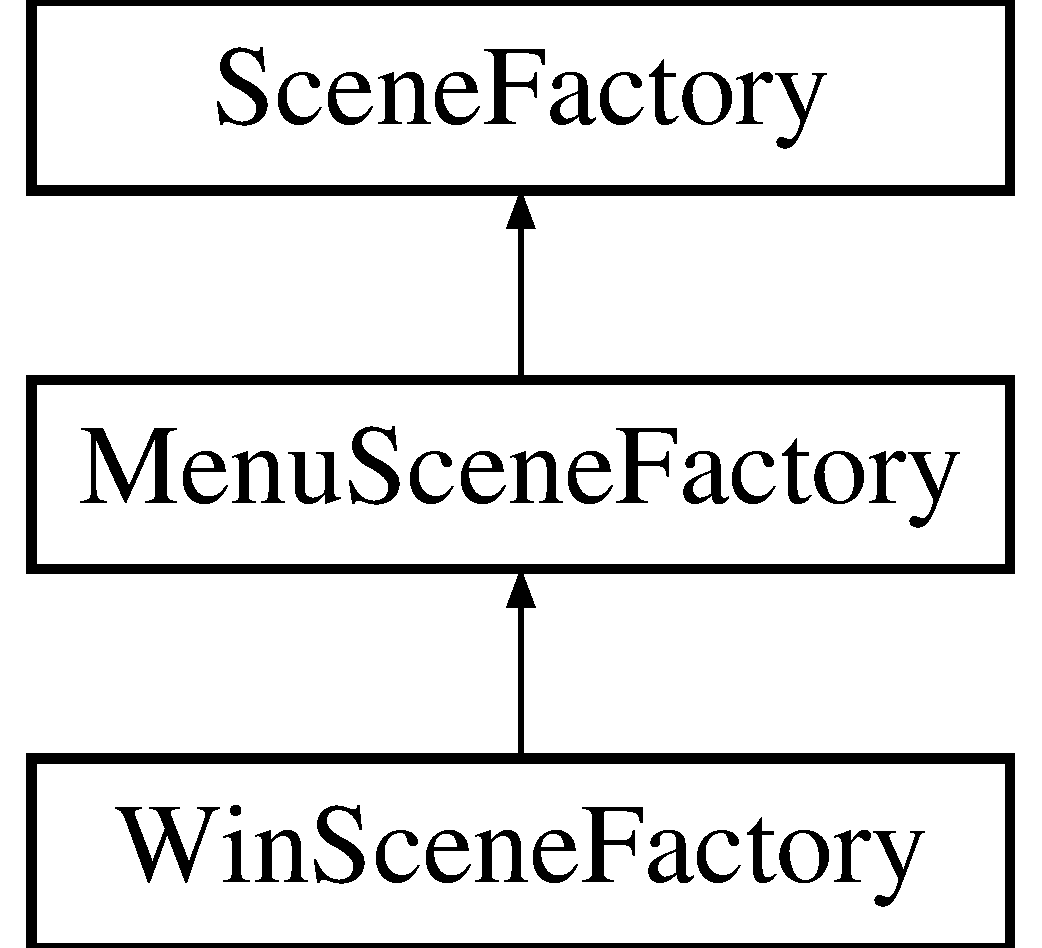
\includegraphics[height=3.000000cm]{d3/db7/class_win_scene_factory}
\end{center}
\end{figure}
\subsection*{Protected Member Functions}
\begin{DoxyCompactItemize}
\item 
\mbox{\Hypertarget{class_win_scene_factory_af2e1c7ae34601b5f4017937d7bd381bb}\label{class_win_scene_factory_af2e1c7ae34601b5f4017937d7bd381bb}} 
virtual std\+::shared\+\_\+ptr$<$ \hyperlink{class_background_factory}{Background\+Factory} $>$ {\bfseries get\+Factory} () const override
\end{DoxyCompactItemize}
\subsection*{Additional Inherited Members}


\subsection{Detailed Description}
Creates the \hyperlink{class_scene}{Scene} that the player goes to when they Win the gam. 

The documentation for this class was generated from the following file\+:\begin{DoxyCompactItemize}
\item 
D\+:/\+Users/\+Tim-\/\+P\+C/\+Documents/\+Software\+\_\+\+I\+I/\+Project/\+Project\+Files/game-\/source-\/code/\+Back\+End\+Systems/Win\+Scene\+Factory.\+h\end{DoxyCompactItemize}

\hypertarget{structxy_vector}{}\section{xy\+Vector Class Reference}
\label{structxy_vector}\index{xy\+Vector@{xy\+Vector}}


Container structure for standardized association of the x-\/y-\/cartesian vector form.  


\subsection*{Public Member Functions}
\begin{DoxyCompactItemize}
\item 
\hyperlink{structxy_vector_a0ee1f276edc4c2aaf1c5973cfe150904}{xy\+Vector} ()
\begin{DoxyCompactList}\small\item\em Default constructor for the \hyperlink{structxy_vector}{xy\+Vector} struct. \end{DoxyCompactList}\item 
\hyperlink{structxy_vector_a06d9403f8df005a7ea3b7765973a93fe}{xy\+Vector} (double X, double Y)
\begin{DoxyCompactList}\small\item\em Constructor for the \hyperlink{structxy_vector}{xy\+Vector} struct. \end{DoxyCompactList}\item 
bool \hyperlink{structxy_vector_a7aca10ebc499fdf7944792741edec285}{operator==} (const \hyperlink{structxy_vector}{xy\+Vector} \&rhs) const
\begin{DoxyCompactList}\small\item\em Simple \hyperlink{structxy_vector}{xy\+Vector} struct equivalency operator overload. For basic struct comparison. \end{DoxyCompactList}\end{DoxyCompactItemize}
\subsection*{Public Attributes}
\begin{DoxyCompactItemize}
\item 
\mbox{\Hypertarget{structxy_vector_a104b718a786e5743e9ab2c76a7b30bbf}\label{structxy_vector_a104b718a786e5743e9ab2c76a7b30bbf}} 
double {\bfseries x}
\item 
\mbox{\Hypertarget{structxy_vector_a9ca5953fcf4a614693e0e56ef5f52ee4}\label{structxy_vector_a9ca5953fcf4a614693e0e56ef5f52ee4}} 
double {\bfseries y}
\end{DoxyCompactItemize}


\subsection{Detailed Description}
Container structure for standardized association of the x-\/y-\/cartesian vector form. 

\subsection{Constructor \& Destructor Documentation}
\mbox{\Hypertarget{structxy_vector_a0ee1f276edc4c2aaf1c5973cfe150904}\label{structxy_vector_a0ee1f276edc4c2aaf1c5973cfe150904}} 
\index{xy\+Vector@{xy\+Vector}!xy\+Vector@{xy\+Vector}}
\index{xy\+Vector@{xy\+Vector}!xy\+Vector@{xy\+Vector}}
\subsubsection{\texorpdfstring{xy\+Vector()}{xyVector()}\hspace{0.1cm}{\footnotesize\ttfamily [1/2]}}
{\footnotesize\ttfamily xy\+Vector\+::xy\+Vector (\begin{DoxyParamCaption}{ }\end{DoxyParamCaption})\hspace{0.3cm}{\ttfamily [inline]}}



Default constructor for the \hyperlink{structxy_vector}{xy\+Vector} struct. 

\begin{DoxyReturn}{Returns}
\hyperlink{structxy_vector}{xy\+Vector} struct by value. 
\end{DoxyReturn}
\mbox{\Hypertarget{structxy_vector_a06d9403f8df005a7ea3b7765973a93fe}\label{structxy_vector_a06d9403f8df005a7ea3b7765973a93fe}} 
\index{xy\+Vector@{xy\+Vector}!xy\+Vector@{xy\+Vector}}
\index{xy\+Vector@{xy\+Vector}!xy\+Vector@{xy\+Vector}}
\subsubsection{\texorpdfstring{xy\+Vector()}{xyVector()}\hspace{0.1cm}{\footnotesize\ttfamily [2/2]}}
{\footnotesize\ttfamily xy\+Vector\+::xy\+Vector (\begin{DoxyParamCaption}\item[{double}]{X,  }\item[{double}]{Y }\end{DoxyParamCaption})\hspace{0.3cm}{\ttfamily [inline]}}



Constructor for the \hyperlink{structxy_vector}{xy\+Vector} struct. 


\begin{DoxyParams}{Parameters}
{\em X} & The x value of the cartesian vector. \\
\hline
{\em Y} & The y value of the cartesian vector. \\
\hline
\end{DoxyParams}


\subsection{Member Function Documentation}
\mbox{\Hypertarget{structxy_vector_a7aca10ebc499fdf7944792741edec285}\label{structxy_vector_a7aca10ebc499fdf7944792741edec285}} 
\index{xy\+Vector@{xy\+Vector}!operator==@{operator==}}
\index{operator==@{operator==}!xy\+Vector@{xy\+Vector}}
\subsubsection{\texorpdfstring{operator==()}{operator==()}}
{\footnotesize\ttfamily bool xy\+Vector\+::operator== (\begin{DoxyParamCaption}\item[{const \hyperlink{structxy_vector}{xy\+Vector} \&}]{rhs }\end{DoxyParamCaption}) const\hspace{0.3cm}{\ttfamily [inline]}}



Simple \hyperlink{structxy_vector}{xy\+Vector} struct equivalency operator overload. For basic struct comparison. 


\begin{DoxyParams}{Parameters}
{\em rhs} & The \hyperlink{structxy_vector}{xy\+Vector} struct valuethat this is compared against. Used by constant reference. \\
\hline
\end{DoxyParams}
\begin{DoxyReturn}{Returns}
boolean of the equivalency. 
\end{DoxyReturn}


The documentation for this class was generated from the following file\+:\begin{DoxyCompactItemize}
\item 
D\+:/\+Users/\+Tim-\/\+P\+C/\+Documents/\+Software\+\_\+\+I\+I/\+Project/\+Project\+Files/game-\/source-\/code/Vector2\+D.\+h\end{DoxyCompactItemize}

%--- End generated contents ---

% Index
\backmatter
\newpage
\phantomsection
\clearemptydoublepage
\addcontentsline{toc}{chapter}{Index}
\printindex

\end{document}
